	%to force start on odd page
	\newpage
	\thispagestyle{empty}
	\mbox{}	
	\section{Electrostatics}
	\lettrine[lines=4]{\color{BrickRed}S}o far we have focus only on the gravitational interaction and the characteristic quantity of matter, named "mass" associated with it. We discussed the electromagnetic interaction, analyzing macroscopic phenomena such as friction, cohesion, elasticity, the forces of contact, etc. Now we look at electronic forces and the characteristic of matter named "\NewTerm{electric charge}\index{electric charge}" associated with them. The electromagnetic interaction binds matter in all its observable forms. It is this that holds the electrons to the nucleus in the atom, which holds together the atoms in molecules, molecules into objects and even your nose to your face...
	
	The "\NewTerm{electric charge}" generate the "\NewTerm{electric force}\index{electric force}" or "\NewTerm{Coulomb force}\index{Coulomb force}\label{coulomb force}" and we are only beginning to understand this force thanks to quantum field theory (see further below in this book). The electric charge is a fundamental concept, which can not be described in terms of more simple and fundamentals concepts. We know it by its effects and unfortunately not by what it is (this was also the case for the mass before the discovery of the Higgs Boson).
	
	Experience has also shown that even if the electric charge is an additive quantity such as the mass, however, it also has negative value (and not exclusively positive as know nowadays for the mass). Thus, in the current language, and as confirmed by experience, two identical sign electric charges repel and two opposite sign electric charges attract (we will see a schematic figure of this further below).
	\begin{figure}[H]
		\centering
		\includegraphics[scale=0.9]{img/electromagnetism/electrostatic_cat.jpg}
		\caption[]{Electric charges exist all around us. They can cause objects to be repelled from each other or to be attracted to each
other. (credit: modification of work by Sean McGrath)}
	\end{figure}
	Let us now see the classic force that is associated with the electric charge:
	
	\subsection{Electric Force}\label{electric force}
	It has experimentally been established by Coulomb that a reference point particle undergoes a force $\vec{F}$ of an intensity proportional to its charge $q$, when placed in the neighborhood of one or more electrical charges $Q_i$ in a medium of absolute electrical permittivity $\varepsilon$ (permittivity to the electric field of course...!) given by in vector notation and non-relativistic:
	
	where $\vec{r}_i$ is the vector position of the sample charge $Q_i$ and $\vec{r}$ of the reference point charge particle relatively to a same orthonormal vector basis.
	
	In other words, two point electric charged particles attract or repel each other in a force directly proportional to their electric charge and inversely proportional to the square of the distance that separates them.
	
	In the case of a system with two particles separated by a distance $r$, we have the same simplified relation and we fall back on the most common form of the electric force or "\NewTerm{Coulomb force}\index{Coulomb force}" as given in most books (as scalar and non-relativistic):
	
	Hence recalling Newton's second law:
	
	Frequently, these relation is defined as the "\NewTerm{Coulomb's law}\index{Coulomb's law}" in most schools and admitted as unprovable. In fact, it is not! This relation can be proved as we will see in the study of quantum fields physics (\SeeChapter{see section Quantum Field Theory page \pageref{yukawa potential}}) using the Klein-Gordon equation in the context of a potential field with spherical symmetry (proof performed by Yukawa).
	
	\begin{tcolorbox}[title=Remark,colframe=black,arc=10pt]
	Don't forget that as $2\pi$ appears frequently in many theorems of physics and mathematics (more than $\pi$ alone), the value $4\pi$ is frequently denoted by $2\tau$ as by definition $\tau=2\pi$.
	\end{tcolorbox}
	In either formulation, Coulomb's law is fully accurate only when the objects are stationary, and remains approximately correct only for slow movement. These conditions are collectively known as the electrostatic approximation. When movement takes place, magnetic fields that alter the force on the two objects are produced. The magnetic interaction between moving charges may be thought of as a manifestation of the force from the electrostatic field but with Einstein's theory of relativity taken into consideration.
	\begin{tcolorbox}[title=Remark,colframe=black,arc=10pt]
	For the relativistic form of Coulomb's law, the reader is referred to the section Special Relativity where it is proved that (vector form):
	
	\end{tcolorbox}
	The value of electric permittivity in vacuum is in turn given experimentally by the "\NewTerm{dielectric constant}\index{dielectric constant}" or simple "\NewTerm{electric constant}\index{electric constant}":
	
	and relatively to medium considered, we define a "\NewTerm{relative dielectric permittivity}\index{relative dielectric permittivity}" $\varepsilon$ that makes it easier to determine the properties of a material with respect to the electric field so that we have the "\NewTerm{absolute electrical permittivity}\index{absolute electrical permittivity}":
	
	It should be mentioned that some authors define the permittivity of vacuum from the speed of light and the magnetic permeability of vaccum (\SeeChapter{see section Magnetostatics page \pageref{magnetic permeability of vacuum}}). Therefore, the value of the electrical permittivity of vacuum is obviously correct by definition. But this only makes sense once known the Maxwell's theory and this will be presented and proved later in the section Electrodynamics (we follow the steps in the historical scientific discoveries).
	
	 It also appears in the Coulomb force constant, as the "\NewTerm{Coulomb constant}\index{Coulomb constant}":
	  
	The factor into parentheses in:
	
	depends only on the distribution of charges $Q_i$ in the volume and the absolute electrical permittivity of the medium $\varepsilon$. Since its value varies from one place to another and depends on the position vector $\vec{r}$ of the reference electric charge, it forms a set of vectors, which property is this of a multitude of electrical field lines hence the use of term "\NewTerm{electric field}\index{electric field}".
	
	The set of these vectors $\vec{E}$ carries therefore the name "electric field", at the point $\vec{r}$ ,developed in the electric charge distribution $Q_i$:
	
	Engineers often use another notation that allows to characterize only the geometry of the field regardless the environment (medium) and for this purpose they introduce the concept of "\NewTerm{displacement field}\index{displacement field}":
	
	We will meet this vector again in the section Electrodynamics during our synthesis of Maxwell's equations.
	
	Coulomb force acting on the sample charge $q$, is then written in a conventional way:
	
	One configuration is of particular interest: two separated point charges of opposite charge. In the limit of vanishing separation, it is named "dipole". Its field fundamentally differs from that of just a single charge even though it is just the sum of the charge. The dipole as a concept is extremely important throughout electrodynamics. It is applied for example explaining the emission of electromagnetic radiation or as a model for molecules.
	
	Let us first consider the case of opposite electric charges. For the given problem we have $\vec{r}_1=-d/2\vec{e}_x$ and $\vec{r}_2=d/2\vec{e}_x$. So the charges lie on the $x$-axis with a separation $d$. Remember that $\vec{e}_x$ is the unit vector in $x$ direction (\SeeChapter{see section Vector Calculus page \pageref{vector calculus}}). The electric field is then given by:
	
	Imagine we are interested in the magnitude and the direction of the field only about the line of the $y$-axis. To figure it out both, we simply calculate:
	
	We see that the electric field has only a component in $x$-direction. Because of the symmetric choice of the coordinate system we could have guessed this in the first place.
	
	The magnitude is therefore given by the norm of the electric field:
	
	Let us now consider the case of equal charges (positive for example):
	
	The direction of the field is in this case always parallel to the $y$-axis but changing sign at $y=0$. Its magnitude is given by:
	
	We find that for equal charges the magnitude of the electric field decreases for large $y$.
	
	With Maple 4.00b we can easily plot these two magnitudes:
	
	\texttt{>plot({1/(0.5\string^2+y\string^2)\string^(3/2),1/(y\string^2)*1/((1/(2*y))\string^2+1)\string^(3/2)},y=-5..5);}
	\begin{figure}[H]
		\centering
		\includegraphics{img/electromagnetism/dipole_profile.jpg}
		\caption{Dipole profile for $q_1=-q_2$ and $q_1=q_2$ along $y$-axis}
	\end{figure}
	This is how looks like some lines of electric field of tow identical charges particles ($q_1=q_2$) with a nice perspective effect:
	\begin{figure}[H]
		\centering
		\includegraphics[scale=1]{img/electromagnetism/3d_dipole.jpg}
		\caption{3D dipole profile with $q_1=q_2$}
	\end{figure}
	
	\pagebreak
	\subsection{Electric Potential}\label{electric potential}
	 Given two points $A$ and $B$ in a region of space where there is an electric field $\vec{E}(x,y,z)$ and given $\Gamma$ a path connecting these two points. So, in the particular case where the source of a field $\vec{E}$ is a sphere or a punctual body and we put  a charge as its neighborhood, we have for the work done by the force to move the charge from point $A$ to point $B$:
	 
	Moreover, this work is as we shall see, equivalent to the potential energy. We thus define the "\NewTerm{potential difference}\index{potential difference}" or simply the "\NewTerm{potential}\index{potential}" by the relation:
	
	and therefore:
	
	And the work can then be written\label{electrostatic potential energy}:
	
	\begin{tcolorbox}[title=Remarks,colframe=black,arc=10pt]
	\textbf{R1.} The potential is often named "\NewTerm{voltage}\index{voltage}" by electricians, electrical engineers and other engineers and the unit of measurement of the potential that is the "\NewTerm{Volt}\index{Volt}" denoted by [V].\\
	
	\textbf{R2.} The potential difference can either exists between two terminals of opposite charge $(+, -)$, or between two terminals of the type $(+, \text{neutral})$ or also $(-, \text{neutral})$. The latter two cases represents typically the configuration used by trains, trams, storms and almost all electromechanical appliances.
	\end{tcolorbox}
	\begin{theorem}
	We will now show in the more general framework that exists that the stationary vector field $\vec{E}$ derivates from a potential field:
	\end{theorem}
	\begin{dem}
	Given a charge $Q$ located relative to a reference frame by the vector $\vec{r}_Q$. Then in each point of space there exists a field $\vec{E}$ such as:
	
	let us develop this expression:
	
	If $\vec{E}$ is a stationary potential field then, there must be a potential $\Phi(x,y,z)$ of this field which satisfies:
	
	Let us look to the potential $\Phi$ exists for a Coulomb field. Then we must have for the field in $x$:
	
	therefore:
	
	and if we do the same development for each component, we also get the same result. Thus the electric potential is a scalar field and not a vector field (the electric field is it obviously a vector field)!
	\begin{flushright}
		$\square$  Q.E.D.
	\end{flushright}
	\end{dem}
	The potential $\Phi(x,y,z)$ is named in the case of a Coulomb field of "\NewTerm{Coulomb potential}\index{Coulomb potential}" and is conventionally chosen such that:
	
	As we can see it by the prior-previous expression of $\Phi(x,y,z)$, $c^{te}$ is an arbitrary constant, which imposes in the case of absence of charges that:
	
	Which finally gives us:
	
	Giving for all components:
	
	that we write in a more condensed way\label{derivation of electric field by the potential}:
	
	\begin{tcolorbox}[title=Remark,colframe=black,arc=10pt]
	The same developments and results (and those that follow) are applicable regarding the gravitational potential field. However, they rarely are made in the literature or schools because the human being does not control (at least until now) the gravitational field with an ease and intensity equivalent to that of the electric field...
	\end{tcolorbox}
	It therefore follows that:
	
	and so for example for a spherical symmetric potential (case that we will find in many other sections of this book), it comes:
	
	
	\pagebreak
	\subsubsection{Path Independance}
	Let us prove now that the potential difference between two points $A$ and $B$ is independent of the path $\Gamma$ traveled such as we did for the gravitational potential field in the section of Classical Mechanics.

	Given $\Gamma$ a path between two points $A$ and $B$ and a field $\vec{E}$ and let us make so that we can express the field on $x$, $y$ and $z$ with respect to a single variable $t$ (which has nothing to do with time...) that would account for its magnitude change for  any movement between these two points:
	
	So with $A$ corresponding to the value $t_1$ of the parametrization and $B$ to the value $t_2$. 
	
	But, we know that (\SeeChapter{see section Differential and Integral Calculus page \pageref{total exact differential}}) that:
	
	Therefore it comes:
	
	Therefore:
	
	This last expression shows that $U$ is independent of the path $\Gamma$ regardless of the way we parametrize it.
	
	The Coulomb field is therefore a "\NewTerm{conservative vector field}\index{conservative vector field}" Indeed, if we consider a closed path $\Gamma$ and $A$ and $B$ are two confused points of the part then the potential difference will be zero!
	
	Notice that sometimes we also say that the gradient of the potential is conservative.

	\pagebreak
	\subsection{Equipotential and Field lines}
	Now we can from what we have built, define the "equipotentials" and "field lines".
	
	Given a Coulomb field defined relatively to a given repository (reference frame). Then at each point $(x, y, z)$ of space, we can associate an electric field vector $\vec{E}(x,y,z)$ and an electric potential.
	
	\textbf{Definition (\#\mydef):} The "\NewTerm{field lines}\index{field lines}" is a family of curves for which the vector $\vec{E}(x,y,z)$ is tangent and constant at each point and the "\NewTerm{equipotentials}\index{equipotentials}\label{equipotentials}" as the lines for which the potential $U (x, y, z)$ are also constant.
	
	\begin{theorem}
	In this case, and that is what we will show, all field lines are perpendicular to all equipotentials if the vector field derived from a potential.
	\end{theorem}
	Let us use the property conservation of the Coulomb field for the proof:
	\begin{dem}
	
	As we are in the presence of an electric field, this therefore derives from a potential as we know. This implies that if the field is not null the potential there is also not. So in the line integral:
	
	one of the terms is zero! This is not the electric field $\vec{E}$ as we in presence of one, which discredits the potential $U$ and as the charge moves $\mathrm{d}\vec{r}$ is not null either. Then write the line integral in another way:
	
	Therefore:
	
	we can then conclude that the equipotential are perpendicular to the lines of the electric field and vice versa. This is what was to be proved.
	\begin{flushright}
		$\square$  Q.E.D.
	\end{flushright}
	\end{dem}
	Here are examples of level lines including field lines and equipotential lines obtained using Maple 4.00b (we will show in our study of differential equations how to get the mathematical functions of the field lines):
	\begin{figure}[H]
		\centering
		\includegraphics{img/electromagnetism/field_and_equpotential_lines_01.jpg}
		\caption[]{Left: a single charge - Right: two charges of the same sign}
		\includegraphics{img/electromagnetism/field_and_equpotential_lines_02.jpg}
		\caption[]{Left: two charges of opposite signs - Right: four charges of the same sign}
	\end{figure}
	\begin{tcolorbox}[title=Remark,colframe=black,arc=10pt]
	Apart from the opposite charges, we recall that the same results are applicable to the masses with the gravitational field!
	\end{tcolorbox}
	Two applications of these results are very important (for which we will limit ourselves to the study of the most important properties):
	\begin{enumerate}
		\item The determination of the field lines and equipotential lines for an infinite straight wire such as we can consider in approximation in the electric circuits or high voltage overhead lines (to determine the influence of fields from wires with their environment - this study is part of the branch of electro-engineering we name EMC for "\NewTerm{ElectroMagnetic Compatibility}\index{ElectroMagnetic Compatibility}"). The results can also be used to determine the "\NewTerm{voltage step}\index{voltage step}" for some rectilinear systems which determines for a given distance, the potential per meter for which a mammal may be killed by electroshock near such a wire. An extension (which I do not wish to deal even if the subject is exciting but very contreversial) is also the influence of this type of potential on the functioning of the human brain in the case of the use of portable phones (antennas transmitting a potential) or about houses near high voltage power lines...
		\begin{tcolorbox}[title=Remark,colframe=black,arc=10pt]
		We will determine in the section of Magnetostatics the Biot and Savart law giving the magnetic field for such a wire carrying a given current intensity.
		\end{tcolorbox}
		
		\item The determination of the field lines and equipotential of an electric dipole has a huge importance in chemistry. We will also see what is the dynamics of it when immersed in a uniform electric field and the energy of interaction between dipoles (as is often the case in chemistry).
	\end{enumerate}
	
	\subsubsection{Infinite straight wire}
	Given:
	
	We have:
	
	by making use of the concept of linear charge density as we have defined it in the section of Principles of Mechanics, we have:
	
	Let us consider an infinite line (wire) of negligible section, and carrying a linear continuous density charge $\gamma$. The goal is then to calculate the electric field and potential at any point $M$ of the space outside this line (wire) in order to know the influences of charges of this line (wire) on the environment by considering the influence of the electric field (if the charges were moving we should also take into account the influence of the magnetic field, which we will do in the section Magnetostatics).
	
	For this, the method is to cut the line (wire) into small elements of line (wire) $\mathrm{d}l$, each element carrying a charge load $\mathrm{d}q$.  The electric field created by the charge load on $P$ at point $M$ located at a distance $x$ and of orthogonal projection $H$ on the line is:
	
	The trick now is to take the symmetric $P'$ of $P$ with respect to $H$ (the orthogonal projection of $M$ on the wire)
	\begin{figure}[H]
		\centering
		\includegraphics{img/electromagnetism/infinite_straight_wire.jpg}
		\caption{Configuration for the analysis of the electrif field of an infinite straight wire}
	\end{figure}
	for which we have identically:
	
	The total field is therefore:
	
	But we have:
	
	Therefore:
	
	As we might expect, the latter relation shows that the field is perpendicular to the line (to the wire...).
	The norm of $\mathrm{d}\vec{E}(M)$ is:
	
	This relation has three dependent variables $r$, $\mathrm{d}l$, $x$. The norm of the total field on a point is equal to the sum of the norms of all the vectors $\mathrm{d}\vec{E}(M)$ of the entire length of the wire since all vectors have the same direction.
	
	For this calculation, we will make a change of variable, and put $r$, $\mathrm{d}l$, $x$ according to the angle $\alpha$ between the line (wire) and the vector $\overrightarrow{PM}$. In the rectangle triangle $HMP$:
	
	if we take the origin of $z$ in $H$. We also have:
	
	and:
	
	therefore:
	
	
	and therefore:
	
	The potential is easily deduced by taking the primitive of $E$ since:
	
	Then we have:
	
	The constant is undetermined since as $r$ approaches infinity, $U$ tends therefore to zero and leads to an infinite constant. This uncertainty is mainly due to the approximation of the infinite wire length.

	\subsubsection{Electric Rigid Dipole}
	An important and interesting disposition of electric charges is that forming an "\NewTerm{electric dipole}\index{electric dipole}" rigorously named "\NewTerm{rigid electric dipole}\index{rigid electric dipole}" or "\NewTerm{electrostatic dipole}\index{electrostatic dipole}". It consists of two equal and opposite electric charges $+ q, -q$ separated by a very small distance. We will seek to determine the potential and the electric field at a point $M$ of the dipole environment.
	
	To determine this let us consider an electric charge $q_i$ on a point $A_i$ and a very distant point $M$ from $A_i$. Let us take an galileen reference frame in O:
	\begin{figure}[H]
		\centering
		\includegraphics{img/electromagnetism/elecrostatic_dipole_study_configuration.jpg}
		\caption{Electric field at a distant point $M$ of the dipole}
	\end{figure}
	The electric potential created at the $M$ by the charge $q_i$ is:
	
	In the triangle $\text{O}A_i M$, the distance $\overline{A_i M}$ can be written with the cosine theorem:
	
	The potential becomes:
	
	At great distance, $r$ becomes much higher than $r_i$, the quantity:
	
	tends to zero. So we can make a Maclaurin development (\SeeChapter{see section Sequences And Series page \pageref{usual maclaurin developments}}) of $(1+u)^{-1/2}$ at the neighborhood of $u=0$. To avoid making heavy calculations, we will limited ourselves to the order two on $r$:
	
	therefore:
	
	Keeping only the terms of the second order in $r$:
	
	The potential becomes:
	
	We kept in the expression of the potential three terms. The term $U_i^0$ is the potential created by a charge that would be in O. In other words, at the zero order, the potential created by a charge located at a point near O is identical to the potential created by a charge that would be in O. The terms $U_i^1,U_i^2$ are correction terms, at the first order and second order respectively. We notice that these terms vary on $1/r^2$ and $1/r^3$, thus decreasing faster than the first. These two terms are thus more effective at smaller distances.
	We see that the terms $U_i^1,U_i^2$ involve the quantity $q_ir_i$. This quantity is what we define as the "\NewTerm{dipole moment}\index{dipole moment}" of the electric rigid dipole:
	
	\begin{tcolorbox}[title=Remark,colframe=black,arc=10pt]
	The dipole moment is expressed in Coulomb meter, but for convenience (...) it is expressed in Debye [D] by some engineers.
	\end{tcolorbox}
	The potential created at great distance by a discrete charge distribution is obtained by summing all individual contributions:
	
	Which can also be written:
	
	By definition, $U_0(M)$ is unipolar or monpolar term, $U_1(M)$ is the dipolar term, $U_2(M)$ is the quadrupolar term. If the electric charge distribution is a globally zero, as is the case of an ideal atom or of an ideal non-ionized molecule, it only remain the multipolar contributions.
	
	Let us return to the particular case of the dipole:
	
	The term monopolar term is zero, since the sum of the electric charges is zero. If we neglect the terms higher than the first order, there remain the dipole contribution.
	
	The angles $\theta_1$ and $\theta_2$ of the dipole are complementary, therefore $\cos(\theta_1)=-\cos(\theta_2)$. But as $q_1=-q_2=q$, the product $q_i\cos(\theta_i)$ is constant.
	
	If the two charges of the dipole are at a constant distance from each other and equidistant from the origin O. We will put that $r_1=r_2=d$.

	The potentiel is therefore reduce to:
	
	
	where $a$ is simply the constant distance between the two electric charges.
	It is customary in the case of the study of the electric dipole to write the above relation as:
	
	where $\vec{p}$ is the definition of the dipolar moment and:
	
	Let us recall now that we proved at the beginning of this section that:
	
	and as we saw in section of Vector Calculus, the gradient in spherical coordinates leads us to write:
	
	therefore:
	
	To determine the equation of the equipotential, remember that these lines (or "surfaces" when in space) are obtained through by the constraint:
	
	Therefore:
	
	with:
	
	The electric field must by definition be tangential to the field lines, thus parallel to the elementary displacement:
	
	Since $E_\phi=0$, we have:
	
	So finally there remains only:
	
	Which is a differential equation that can be easily integrate:
	
	Which is equivalent to write:
	
	The plot of the field and equipotential lines then gives in spherical coordinates (remember that the vertical component is zero by symmetry):
	\begin{figure}[H]
		\centering
		\includegraphics{img/electromagnetism/dipole_electric_equipotentials.jpg}
		\caption{Polar plot of the field lines and equipotentials of an electric dipole}
	\end{figure}
	Even if in an electric dipole the two charges are equal and opposite, giving a zero net charge, the fact they are slightly displaced is sufficient to produce a non identically zero electric field. In atoms, the center of mass of the electrons coincides with the core, and therefore the average electric dipole moment of the atom is zero. But if an external field is applied, the movement of electrons is distorted and the electron mass center is displaced by a given distance from the core. The atom is then polarised and becomes an electric dipole of moment $\vec{p}$. This moment is proportional to the external applied field $\vec{E}$.

	As we did not found in Maple 17.00 how to do the polar plot above here is another Maple 17.00  code to have fun with a dipole:
	
	\texttt{>V:=1/sqrt((x-1)\string^2+y\string^2+z\string^2)-2/sqrt((x+1)\string^2+y\string^2+z\string^2):\\
	>with(LinearAlgebra); with(VectorCalculus); with(plots);\\
	>with(plottools);\\
	>Efield := Gradient(-V, [x, y, z]);\\
	>fieldplot3d([Efield[1], Efield[2], Efield[3]],x =-1.5..1.5, y =-1.5..1.5, z =-1.5..1.5);\\
	>NormEfield := Normalize(Efield,2);\\
	>p1:=sphere([1, 0, 0],0.75,color=red);\\
	>p2:=sphere([-1, 0, 0],1.5,color=blue);\\
	>p3:=fieldplot3d(NormEfield,x=-4.5..4.5,y=-4.5..4.5,z =-4.5..4.5,color=black);\\
	>display([p1, p2, p3], scaling = constrained);
	}

	Giving at first (obviously the dimensions are fictitious):
	\begin{figure}[H]
		\centering
		\includegraphics{img/electromagnetism/dipole_electric_field_maple.jpg}
		\caption{Electric field lines for two charges of opposite signs with Maple 17.00}
	\end{figure}
	Or to get the view of the potential weel with the equipotentials:

	\texttt{>z:= 0;\\
	>plot3d(V,x =-1.5..1.5, y=-1.5..1.5, style=patchcontour,contours=200);
	}

	\begin{figure}[H]
		\centering
		\includegraphics{img/electromagnetism/dipole_potential_well.jpg}
		\caption{Potential well and equipotentiels of the dipole with Maple 17.00}
	\end{figure}
	Or to get a 2D profile of the electric field and equipotentials:
	
	\texttt{>p4:=implicitplot({seq(V=(1/10)*b,b=-10..10)},x=-5..5,y=-4..4);\\
	>p5:=fieldplot([NormEfield[1],NormEfield[2]],x=-5 .. 5,y=-4..4); 
	\\>display([p4, p5], scaling = constrained);\\
	}
	\begin{figure}[H]
		\centering
		\includegraphics{img/electromagnetism/dipole_potential_field_profile_maple.jpg}
		\caption{2D profile of electric field and potential of the dipole with Maple 17.00}
	\end{figure}
	\begin{tcolorbox}[title=Remark,colframe=black,arc=10pt]
	Molecules also may have a permanent electric moment. Such molecules are named "\NewTerm{polar molecules}\index{polar molecules}" For example, in the HCl molecule the electron of the hydrogen atom spends more time to move around the chlorine that around the hydrogen atom. Also, the center of negative charges does he not coincide with that of the positive charge of the center and the molecule has a dipole moment. By cons, in the molecule $\text{CO}_2$, all the atoms are aligned, and the resulting electric dipole moment is zero for reasons of symmetry.
	\end{tcolorbox}
	When an electric dipole is positioned in an electric field, a force is exerted on each of the charges of the dipole. The resulting force is:
	
	Let us consider the particular case where the electric field is directed along the $x$-axis and where the dipole is oriented parallel to this field. If we only consider the quantities:
	
	with $a$ being the distance between the two charges, and therefore:
	dipole is oriented parallel to this field. If we only consider the quantities:
	
	This result show that an electric dipole oriented parallel to the field tends to move in the direction in which the field increases (as the gradient thereof). We note that if the electric field is uniform, the resultant force on the dipole is zero!!!
	
	The potential energy of the dipole is:
	
	If we use the equation:
	
	to describe the uniform electric field and if $\theta$ is the angle between the dipole and the electric field, the last factor $(U_+ - U_-)/a$ is just the component $E_a=E\cos(\theta)$ of the field $\vec{E}$ parallel to $a$. So:
	
	or:
	
	The potential energy is minimum for $\theta=0$, which shows that the dipole is in equilibrium when it is oriented parallel to the field.

	These configurations of a dipole placed in an electric field have very important applications. For example, the electric field of an ion in a solution polarized the solvent molecules that surround the ions and they are oriented as in the figure below:
	\begin{figure}[H]
		\centering
		\includegraphics{img/electromagnetism/dipole_solvant.jpg}
		\caption{Example of what happens in a solution with an ion}
	\end{figure}
	In a solvent with polar molecules such as water, ions of an electrolyte in solution are surrounded by a number of these molecules due to the dipole-charge interaction. This phenomenon is named "solvation" of the ion, specifically "hydration" if the solvent is water.
	
	For example with Salz (NaCl):
	\begin{figure}[H]
		\centering
		\includegraphics{img/electromagnetism/nacl_hydration.jpg}
		\caption[Hydration of Salz]{Hydration of Salz (source: ?)}
	\end{figure}
	These oriented molecules become more or less dependant of the ion, increasing its effective mass and decreasing its effective charge, which is partially obscured by the molecules (screening). The net effect is that the mobility of a ion in an external field is reduced. Similarly, when a gas or liquid, which  molecules are permanent dipoles is placed in an electric field, the molecules as a result of the force couple applied due to the electric field, tend to align with their dipoles parallel. We then say that the substance was "\NewTerm{polarized}\index{polarized}".

	It may therefore be interesting to determine the vector electric field produced by a dipole rather than its potential. The electrostatic field created at a point $M$ by the doublet is obtained by performing the vector sum of the fields created in this point by positive $P$ and negative $N$ charges, hence:
	
	The distribution of charges being invariant by rotation about the $z$ axis of the doublet, the topography is independent of the azimuthal angle $\pi$ of the spherical coordinates. We can then represent it in any meridian plane passing through the axis $NP$. The field $\vec{E}$ is the given by:
	
	Having:
	
	vectorially, we get:
	
	The dot product being the multiplication of components one by one, we have:
	
	Hence:
	
	Finally:
	
	So by a limited Maclaurin series development as we did at the beginning:
	
	By introducing:
	
	We can simplify the notations:
	
	It may also be relevant to calculate the energy of interaction between two electric dipoles. If we denote by $\vec{p}_1$ the dipole moment, we can write:
	
	If we denote by $\vec{p}_2$ the moment of the second dipole and if we use the relation:
	
	we find that the interaction energy between two dipoles is:
	
	We can draw out several important conclusions from this result. The energy of interaction $E_{P,1,2}$ is symmetric relatively to the two dipoles, because the permutation of $\vec{p}_1$ and of $\vec{p}_2$ leaves it unchanged. This is an expected result. The interaction between two dipoles is not central as it depends of the angles which the vector position or the unitary vector $\vec{u}_r$ do with $\vec{p}_1$ and $\vec{p}_2$.
	
	An atom, molecule or a ion, whose dipole moment is zero in the fundamental state, acquire a dipole moment under the action of the applied non-uniform electric field as we have seen since the opposing signs charges are sollicited in opposed directions. The centers of gravity of positive and negative charges do not coincide anymore, it appears an "\NewTerm{induced dipole moment}\index{induced dipole moment}". 

	In an experiment with linear approximation for weak excitatory electric fields, the induced dipole moment is proportional to the applied field $\vec{E}$, which we translate by  (it is in fact an approximation of the Langevin-Debye relation we will prove later):
	
	The quantity $\alpha$, which physical dimension is that of a volume is the "\NewTerm{polarizability}\index{polarizability}" of the structure. The dipole-dipole electrostatic interaction was introduced by J.D. Van der Waals in 1873, in the case of molecules, to interpret real deviations from the ideal gas.
	
	The Van der Waals forces are repulsive as the distance between molecules is very low because they oppose the interpenetration of electron clouds, what we express by introducing their volume (covolume).

	By cons, they are attractive when the distance is sufficient. We attribute this attraction to three types of interactions involving rigid or induced dipoles:
	\begin{enumerate}
		\item The forces between polar molecules (rigid dipoles), say to be "\NewTerm{Keesom forces}\index{Keesom forces}".

		\item The forces between a polar molecule (rigid dipole) and a polarizable molecule (induced dipole) named "\NewTerm{Debye forces}\index{Debye forces}".

		\item	The average forces between induced dipoles which appear even when the molecules are not polar, named "\NewTerm{London forces}\index{London forces}".
	\end{enumerate}
	In all these three cases, the electrostatic energy is negative (attraction) and varies as $r^{-6}$. To prove this statement, let us calculate the interaction energy between two rigid dipoles, of dipolar moments $\vec{p}_1$ and $\vec{p}_2$:
	
	with:
	
	and:
	
	Therefore:
	
	This is the van der Waals interaction potential between two dipoles atoms where $C_6$ is the "\NewTerm{Van der Waals constant}\index{Van der Waals constant}".
	
	Hence:
	
	Thus, the radial dependence of the force is indeed in $r^{-7}$. This very rapid decay of the Van der Waals force with distance helps explain its very short range and therefore its influence when the medium is sufficiently dense. However the decay is slower than the chemical bond that deacrease exponentially (\SeeChapter{see section Quantum Chemistry page \pageref{molecular chemistry}}).
	\begin{tcolorbox}[title=Remark,colframe=black,arc=10pt]
	The interaction between polar molecules, of the Keesom type, is made very high in the presence of hydrogen, because the latter, thanks to its small size, also interacts with the atoms of other molecules. It is that one which is at the origin of the "\NewTerm{hydrogen bonding}\index{hydrogen bonding}".
	\end{tcolorbox}
	
	\subsection{Electric Field Flow}
	Given $\vec{V}$ a vector field and $S$ a surface named "\NewTerm{Gauss surface}\index{Gauss surface}" in space. If we divide this area into a number $N$ of smaller surfaces $\mathrm{d}S$ each traversed by a field $\vec{V}_i$ and having a unit perpendicular vector $\vec{n}_i$ (special case) on their surface, then we can form the sum of:
	
	When $N$ tends to infinity and all $\mathrm{d}S$ to zero, we get for this sum:
	
	The value of this integral thus gives the flow $\Phi_V$ of the field $\vec{V}$ through the surface $S$ delimited by a domain $\Lambda$ and where:
	
	In the case of the electrostatic field, we write:
	
	This expression, define the "\NewTerm{electric flow}\index{electric flow}" or also named "\NewTerm{electric flux}\index{electric flux}".	
	
	The inevitable question that arises is then: what is its physical meaning? The flux of a fluid is the amount of fluid (especially the quantity of volume) passing through a surface by second. Then there is a flux (flow) of something. About the electrical flux (flow), from the classical point of view, nothing flows, the electric field is already established and is static, but is flow through the surface. The value of the electric field at any point in space is the field intensity at that point, while the flow can be considered the quantity of field which passes through the surface $S$. 

	There is a hundred years, physicists identified the flow with the number of electric field lines passing through the surface. But the least we can say is that the simplistic view that the field lines have a distinct reality and that we can count is misleading. We will see during our study of Quantum Field Theory, in the section of the same name, that the latter supports a virtual photons current that is the nature of electromagnetic interactions. Despite this, the physicists did not hurry to associate the flow of virtual photons of the 20th century to the continuous electric field lines of the 19th century. Whatever its nature, the concept of flow is powerful and of great practical use, both in electricity and magnetism.
	
	As will we prove it in the framework of Maxwell's equations (\SeeChapter{see section Electrodynamics page \pageref{maxwell equations}}), solving this integral gives in the general case (this is the "Gauss law for electrostatic\index{Gauss law for electrostatic}" also named "Gauss theorem for electrostatic"):
	
	In the case where the surface is not closed and reduce to a plane, the previous close surface integral is reduced to:
	
	
	\subsubsection{Capacitor}\label{capacitor}
	A capacitor (originally known as a condenser) is a passive two-terminal electrical component used to store electrical energy temporarily in an electric field. The forms of practical capacitors vary widely, but all contain at least two electrical conductors (plates) separated by a dielectric (i.e. an insulator that can store energy by becoming polarized). The conductors can be thin films, foils or sintered beads of metal or conductive electrolyte, etc. The nonconducting dielectric acts to increase the capacitor's charge capacity. Materials commonly used as dielectrics include glass, ceramic, plastic film, air, vacuum, paper, mica, and oxide layers. Capacitors are widely used as parts of electrical circuits in many common electrical devices. Unlike a resistor, an ideal capacitor does not dissipate energy. Instead, a capacitor stores energy in the form of an electrostatic field between its plates.

	When there is a potential difference across the conductors (e.g., when a capacitor is attached across a battery), an electric field develops across the dielectric, causing positive charge $+Q$ to collect on one plate and negative charge $-Q$ to collect on the other plate. If a battery has been attached to a capacitor for a sufficient amount of time, no current can flow through the capacitor. However, if a time-varying voltage is applied across the leads of the capacitor, a displacement current can flow.

An ideal capacitor is characterized by a single constant value, its capacitance. Capacitance is defined as the ratio of the electric charge $Q$ on each conductor to the potential difference $U$ between them. The SI unit of capacitance is the farad [F, which is equal to one coulomb per volt ($1$ [C$\cdot$V$^{-1}$]). Typical capacitance values range from about $1$ [pF] to about $1$ [mF].

	The larger the surface area of the "plates" (conductors) and the narrower the gap between them, the greater the capacitance is. In practice, the dielectric between the plates passes a small amount of leakage current and also has an electric field strength limit, known as the breakdown voltage. The conductors and leads introduce an undesired inductance and resistance.

	Capacitors are widely used in electronic circuits for blocking direct current while allowing alternating current to pass. In analog filter networks, they smooth the output of power supplies. In resonant circuits they tune radios to particular frequencies. In electric power transmission systems, they stabilize voltage and power flow.
	\begin{figure}[H]
		\centering
		\includegraphics[scale=0.25]{img/electromagnetism/capacitors.jpg}
		\caption[Some capacitive dipoles]{Some capacitive dipoles (source: Martin Bircher http://www.e-style.ch)}
	\end{figure}
	As a direct application of Gauss's theorem, very useful in electronics and for engineers, consider a large thin a flat sheet, wearing a homogeneous surfacic electronic charge density $\sigma$ and immersed in an environment of absolute electrical permittivity $\varepsilon$. In the area close to its center, the electric field resulting from all the fields of the fields is normal, uniform, constant and go away from the sheet. Let us consider a Gaussian surface with a cylinder shape limited by the bases $S_1=S_2=S$ and its tubular surface $S_3$ symmetrical with respect to the sheet. It therefore encloses an electric charge $\sigma S$. It follows that:
	
	and as $E=E_1=E_2$ and $E_3=0$, we find:
	
		Finally, the electric field of a large and thin loaded flat sheet is:
	
	If we put face to face two identical plates but with opposite charges, the algebraic sum will of course be:
	
	Excepted of the extremities where the side effect is important, the overall field is everywhere the vector sum of uniform fields from two opposing thin loaded layers. We name such a system a "\NewTerm{plane and parallel capacitor}\index{plane and parallel capacitor}":
	\begin{figure}[H]
		\centering
		\includegraphics{img/electromagnetism/plane_capacitor.jpg}
		\caption{Schematic diagram of plane and parallel capacitor}
	\end{figure}
	The result is remarkable because it is independent of the distance between the planes (in fact never forget it is an approximation for very small distances!). The calculation of electric potential is therefore simplified. Thus:
	
	Thus, the capacitance of the plane and parallel capacitor is consequently:
	
	Let us now recall that we have shown previously that:
	
	Since each plate of a parallel and plane capacitor contributes equally, the total electric field between the plates would be :
	
	The potential difference is:
	
	Solving for $Q$ yields:
	
	The plates are oppositely charged, so the attractive force $F_\text{att}$ between the two plates is equal to the electric field produced by one of the plates times the charge on the other:
	 
	This is therefore the force between the plates of a parallel (infinite) plate capacitor.
	
	The plates of a cylindrical capacitor are two infinite rolled cylinders (or very long relatively to their diameter), coaxial of respective radius $R_1$ and $R_2$. It is therefore the very important case of the coaxial cable (which dielectric is often polyethylene) that we can found in many laboratories (and not only!):
	\begin{figure}[H]
		\centering
		\includegraphics{img/electromagnetism/capacitors_cylindrical.jpg}
		\caption{Schematic diagram of cylindrical capacitor}
	\end{figure}
	Let us see a second academic example that is the "\NewTerm{cylindrical capacitor}\index{cylindrical capacitor}":

	By Gauss theorem, we know that:
	
	And since the field $\vec{E}$ is collinear at every point of the surface $\vec{S}$, it immediately comes by knowing the expression of the surface of the cylinder (\SeeChapter{see section Geometric Shapes page \pageref{cylinder}}):
	
	But:
	
	Therefore:
	
	
	Let us also calculate the capacity of a spherical capacitor which corresponds in a first approximation to some of Van Der Graaf generators that we have in the labs of some schools, museums or even research centers...
	
	A "\NewTerm{spherical capacitor}\index{spherical capacitor}" consists of two concentric spheres of radius $R_1$ and $R_2$ with $R_1<R_2$.
	\begin{figure}[H]
		\centering
		\includegraphics{img/electromagnetism/capacitors_spherical.jpg}
		\caption{Schematic diagram of spherical capacitor}
	\end{figure}
	We now have immediately:
	By Gauss theorem, we know that:
	
	And therefore since the field is assumed to be colinear at any point on the surface it comes immediately knowing the expression of the surface of a sphere:
	
	But:
	
	Then we have:
	
	Then we have:
	
	And thats all for the classical examples...
	
	Well! We have just seen that the capacity was defined as:
	
	or in alternative current notation (when the current or the voltage varies as function of the time, it is the usage to write them in lowercase):
	
	We then have for the instantaneous power (\SeeChapter{see section Electrokinetics page \pageref{electromotive force}}):	
	
	Assuming an ideal capacitor (which does not dissipate energy by Joule effect) we get:
	
	
	This energy is always positive and is stored in electrostatic form in the capacitor.
	
	In the context of a sine wave alternative current, the average power will be equal to zero. We can generalize this by assuming that a perfect capacitor does notdissipate power no Joule effect.
	\begin{tcolorbox}[title=Remark,colframe=black,arc=10pt]
	Some scientific experiments requiring enormous energy use thousands of giant capacitors charged in the long term to accelerate particles or to make operate megajoules LASER. However we can not actually store the surplus of electric power of some power plants, which is why we use this surplus to pull back the water in the dams that can use their pool as a reserve of potential energy to produce a complement to electricity at the time of peak consumption (inverse transformation). We can also found huge capacitor that have for purpose to manage critical voltage collapse in a changing environment (this are the big cylinder in transformation stations).
	\end{tcolorbox}
	
	
	\paragraph{Dielectric strength}\mbox{}\\\\
	The term "\NewTerm{dielectric strength}\index{dielectric strength}" denoted $\mathcal{R}$ and that for SI units volts per meter [V$\cdot$m$^{-2}$] has the following meanings:
	\begin{itemize}
		\item Of an insulating material, the maximum electric field that a pure material can withstand under ideal conditions without breaking down (i.e., without experiencing failure of its insulating properties).
		
		\item For a specific configuration of dielectric material and electrodes, the minimum applied electric field (i.e., the applied voltage divided by electrode separation distance) that results in breakdown.
	\end{itemize}
	The theoretical dielectric strength of a material is an intrinsic property of the bulk material and is independent of the configuration of the material or the electrodes with which the field is applied. This "intrinsic dielectric strength" corresponds to what would be measured using pure materials under ideal laboratory conditions. At breakdown, the electric field frees bound electrons. If the applied electric field is sufficiently high, free electrons from background radiation may become accelerated to velocities that can liberate additional electrons during collisions with neutral atoms or molecules in a process named "avalanche breakdown". Breakdown occurs quite abruptly (typically in nanoseconds), resulting in the formation of an electrically conductive path and a disruptive discharge through the material. For solid materials, a breakdown event severely degrades, or even destroys, its insulating capability.

	The factors affecting apparent dielectric strength are typically:
	\begin{itemize}
		\item it decreases with increased sample thickness.
		\item it decreases with increased operating temperature.
		\item it decreases with increased frequency.
		\item for gases (e.g. nitrogen, sulfur hexafluoride) it normally decreases with increased humidity.
		\item for air, dielectric strength increases slightly as humidity increases
	\end{itemize}
	For a capacitor used in electronics, if we exceed the dilectric strenght value, we observe the destruction of the element. This maximum value of the voltage applied to the terminals, is named sometimes the "\NewTerm{breakdown voltage}\index{breakdown voltage}" of the capacitor and denoted $U_c$ . We can define the dilectric strength of the material (medium) as:
	
	\begin{tcolorbox}[colframe=black,colback=white,sharp corners]
	\textbf{{\Large \ding{45}}Example:}\\\\
	Two common dielectric strength values that have to be know by students are:
	
	\end{tcolorbox}
	When we talk of dielectric strength, we also speak of the dielectric is an insulator or a substance that does not conduct electricity and is polarizable by an electric field. In most cases, the dielectric properties are due to the polarization of the substance. When the dielectric (in this case, air is the dielectric) is placed in an electric field, the electrons and protons of its atoms are reoriented and, in some cases, at the molecular level, a polarisation is induced (as we have seen in our study of the dipoles above). This polarization produces a potential difference, or voltage, between both terminals of the dielectric; it then stores the energy which becomes available when the electric field is removed. The effectiveness of a dielectric is its relative ability to store energy compared to that of vacuum. It is expressed by the relative electric permittivity $\varepsilon_r$, determined relative to that of a vacuum $\varepsilon_0$. The dielectric strength is then ability of a dielectric to withstand electric fields without losing its insulating properties. An effective dielectric releases a big fraction of the energy it had stored when the electric field is reversed.
	
	\subsection{Electrostatic potential energy}\label{electrostatic potential energy}
	Let us consider two electric charges $q_1,q_2$. The first is supposed to be at rest and fixed; the second is brought from infinity to a distance $a$ from $q_1$ (the same reasoning was applied to the gravitational field in the section of Classical Mechanics!). Suppose that the two charges are of the same sign. As $q_1,q_2$ tend to repel each other, we have to provide a potential energy $E_p$ to take $q_2$ (infinitely slowly) of $q_1$. The work $\mathrm{d}W$ done by the electrostatic force at any point is by definition as we know:
	
	The potential enery of the system is:
	
	as the force $F$ is resistive (hence the origin of the sign "$-$").

	Therefore:
	
	We then get the potential energy at a point ($x$ in the numerator is simplified with an $x$ in the denominator) to a given sign convention:
	
	If we have $q_2=Zq_1$ where $Z \in\mathbb{N}$ and we denote $q_1=e$ then we fall back on a well known way to write the previous relation:
	
	If the path is not linear we have obviously as in Classical Mechanics with the electric field and using the notations seen at the begining of the section:
	
	Notice that:
	
	can also be written as:
	
	\begin{tcolorbox}[title=Remark,colframe=black,arc=10pt]
	Caution! When do physics, we have to be sure what potential energy we are about talking. This is a major problem! If you take for example the potential energy due to gravitational force, it can take any value depending on the reference point. If the reference is at sea level, a point below the sea level will have a negative potential energy, by cons if the reference is the center of the Earth, there will be only positive potential energies. That is why we are writing rather the potential energy in the form of height difference relative to a reference in mechanics. For the potential energy of the electron, we must know with what it interacts. If it is with a negative charge, the product of the electric charge values will be positive and therefore the potential energy of interaction will be positive, if it interacts with a positive charge, the product will be negative and the potential energy will be negative. In short, we must know what we are talking about. This is an example where words are important in physics too (same problems as the foundations of mathematics!).\\
	
	In general, if the potential energy decreases when the distance increase, the force is repulsive if it increases when the distance increse, the force is attractive.
	\end{tcolorbox}
	
	\begin{flushright}
	\begin{tabular}{l c}
	\circled{90} & \pbox{20cm}{\score{3}{5} \\ {\tiny 75 votes,  66.13\%}} 
	\end{tabular} 
	\end{flushright}

	%to force start on odd page
	\newpage
	\thispagestyle{empty}
	\mbox{}	
	\section{Magnetostatics}
	\lettrine[lines=4]{\color{BrickRed}M}agnets are known since ancient times (without that it was known at that the origin of their properties) under the name "magnetite": black stones found near the city of Magnesia (Turkey). This is from this stone that also comes the current name of the "magnetic field". The Chinese were the first to use the properties of the individual magnets more than 1,000 years before for compasses. They consisted of a magnetite needle resting on straw floating on the water contained in a graduated container.
	
	Magnetostatics is the study of magnetic fields in systems where the currents are steady (not changing with time). It is the magnetic analogue of electrostatics, where the charges are stationary. The magnetization need not be static; the equations of magnetostatics can be used to predict fast magnetic switching events that occur on time scales of nanoseconds or less. It is even a good approximation when the currents are not static - as long as the currents do not alternate rapidly.
	
	As for the electric field, a good/better understanding of the origin of this field can be done through modern theories such as wave quantum physics and quantum field theory. The beginner reader will have therefore to be patient, as for the study of the electric field, until to get in this book the knowledge to study these modern theories.
	
	The quantitative study of the interactions between magnets and currents was made by the physicists Biot and Savart in 1820 only (nobody knew before that the compass was influenced by the current inside the core of the Earth). They measured the amplitude of the oscillations of a magnetic needle according to its distance to a straight current. They found that the force acting on a pole is directed perpendicular to the direction connecting the center to this conductor wire and it varies inversely with the distance. This is the first case that we will study.
	
	The idea of the experiment was the following:
	\begin{figure}[H]
		\centering
		\includegraphics[scale=0.9]{img/electromagnetism/biot_savart.jpg}
	\end{figure}
	\pagebreak
	Or in real life with a much simple configuration:
	\begin{figure}[H]
		\centering
		\includegraphics{img/electromagnetism/biot_savart_simple.jpg}
	\end{figure}
	Given a movement of electric charges (i.e.: a current $I$) generating in the space a vector field whose effects are measurable and whose properties differ from those of the electrostatic field. We deduce the existence of a new vector field we name (temporarily) "\NewTerm{magnetic field}\index{magnetic field}" and which we denote by $\vec{B}$.
	
	The physical units of the magnetic field will naturally been deduced from the time we will be able to connect this magnetic field to something known as a Force for example . This is what we will see further below during our study of the "Laplace Force".
	
	The simplest case of study consisting of an indefinite straight conductor wire (example that we can also assimilate to a simple move of charges without having necessarily a wire to carry them) carrying a current $I$ (see the section Electrokinetics for the concept of "current") shows that the magnetic field lines are circles having for axis the conductor wire itself:
	\begin{figure}[H]
		\centering
		\includegraphics{img/electromagnetism/ampere_wire.jpg}
		\caption{Magnetic field around a straight infinite wire}
	\end{figure}
	The direction of $\vec{B}$ is usually defined by the intermittance of "\NewTerm{Ampère's observer}\index{Ampère's observer}", that is to say, an observer that would be positioned along the wire, so that the current goes to its feet towards its head and who would look at the point $M$ where we evaluate the magnetic field. The field $\vec{B}$ is directed from the right to the left of this observer. This is represented many times by the following had figure:
	\begin{figure}[H]
		\centering
		\includegraphics{img/electromagnetism/ampere_observer.jpg}
		\caption{Ampere observer hand rule}
	\end{figure}
	It is said that is was experimentally established by Biot and Savart in 1820 that the norm of the magnetic field $\vec{B}$ at the distance $r$ of the wire is proportional to the current $I$ running through it and inversely proportional to $r$ such that:
	
	This relation is traditionally considered as the pillar of the study of the magnetic field.
	
	The proportionality coefficient $k$ depends as always to selected unit system (as for other study fields). For the set of all its consequences, it is advantageous to write the above expression in a form that makes appear the perimeter of the circle of radius $r$. So we put:
	
	\begin{tcolorbox}[title=Remark,colframe=black,arc=10pt]
	Don't forget that as $2\pi$ appears frequently in many theorems of physics and mathematics (more than $\pi$ alone), this value is frequently denoted by the letter $\tau$.
	\end{tcolorbox}
	Thus we obtain the value of the magnetic field at a distance $r$ from a straight conductor wire through which a constant current $I$ pass through:
	
	where $\mu_0$ is a new constant which we name "\NewTerm{magnetic permeability of vacuum}\index{magnetic permeability of vacuum}\label{magnetic permeability of vacuum}" (again as for for the electrical permittivity, there is a "\NewTerm{relative magnetic permeability}\index{relative magnetic permeability}") and whose value is given as usual in this book with the other physical constants in the section Principles of Mechanics chapter.
	
	The units of this constant, even if given in the section Principias of the Mechanics chapter, will be deducted automatically as soon as we have managed to link the magnetic field with the concept already known of "Force" (see below). This is what we will see when we will study the "\NewTerm{Laplace Force}".
	
	\subsection{Ampere's theorem }
	In classical electromagnetism, the "\NewTerm{Ampère's theorem}\index{Ampère's theorem}" or "\NewTerm{Ampère's circuital law}\index{Ampère's circuital law}" or simply "\NewTerm{Ampère's law}\index{Ampère's law}" relates the integrated magnetic field around a closed loop to the electric current passing through the loop.
	
	It is interesting to calculate the "\NewTerm{circulation of the magnetic field}\index{circulation of the magnetic field}" $\vec{B}$ in vacuum (or not) along a contour $\Lambda$ that turns once in the positive direction (anti-clockwise) around the wire oriented in the direction of the current (Ampere observer):
	
	
	\begin{tcolorbox}[title=Remark,colframe=black,arc=10pt]
	The field is collinear along the path as we have seen previously hence the fact that the dot product can be written as a simple product of norms.
	\end{tcolorbox}
	We obtain then by definition the "\NewTerm{Ampère's law}\index{Ampère's law}" (or erroneously named "\NewTerm{Ampère's theorem}\index{Ampère's theorem}" because this result is not provable ... at least as far as we know...):
	
	where the current $I$ in a high symmetry system can be assimilated to a simple algebraic sum of currents snared by the path such that we have:
	
	Warning!!! This is not because the circulation of the magnetic field is zero in a region of space that the magnetic field is zero at any point!
	\begin{tcolorbox}[title=Remarks,colframe=black,arc=10pt]
	\textbf{R1.} The Ampere's law will give us the possibility to determine the fourth Maxwell equation that we will prove in the section of Electrodynamics.\\
	
	\textbf{R2.} The prior-previous relation is sometimes wrongly named "Ampere theorem" when in fact this result is not provable as already mentioned. Some physicists, however, use the fourth Maxwell equation to prove the prior-previous relation but then this is the snake biting its tail...
	\end{tcolorbox}
	The expression that we obtained can be simplified even more if we introduce a new physical being named "\NewTerm{magnetic field intensity}\index{magnetic field intensity}" or more commonly "\NewTerm{magnetic excitation}\index{magnetic excitation}" and which is denoted by the letter $\vec{H}$ (which is intrinsically independent of the propagation medium!).
	
	If we consider that we are always in the vacuum where there is no magnetic dipole then we define it in the vacuum by:
	
	Therefore, we are often taken to speak about "\NewTerm{magnetic induction}\index{magnetic induction}" for $\vec{B}$ and "\NewTerm{magnetic field}\index{magnetic field}" for $\vec{H}$. But both are happily confused following the authors/professors/teachers and especially depending on the contexts (as will be the case also in this book). When we deal with magnets that have intrinsic magnetization by the properties of the material that are made from, we denote distinctly the external magnetic field by:
	
	which is a more general form of the previous relation. It is therefore usual to define the "\NewTerm{magnetic susceptibility}\index{magnetic susceptibility}" as being the dimensionless ratio:
	
	Thus, the magnetic susceptibility indicates the amplitude with which a material responds magnetically to the presence of a magnetic excitation. We then get by this definition, the relation between relative magnetic permeability and magnetic susceptibility:
	
	Therefore:
	
	where $\mu$ is named the "\NewTerm{absolute magnetic permeability}\index{absolute magnetic permeability}".
	
	It is customary to name materials that have a positive magnetic susceptibility "\NewTerm{paramagnetic materials}\index{paramagnetic materials}" (contributing to increase the magnetic field) and those with a negative magnetic susceptibility "\NewTerm{diamagnetic materials}\index{diamagnetic materials}" (tend to oppose to the magnetic field ). We will see later the Langevin theoretical models to explain quantitatively with a relatively good approximation the two phenomena (in both cases the magnetic susceptibility has a value which is very low).
	
	So finally we can also write the Ampere's Law as following:
	
	The interest of the Ampere's law and of the concept of circulation of the magnetic field may appears like this more evident.
	
	This latter relation obviously is obviously very useful in theoretical physics because it will allow us to determine other important powerful results. Otherwise, in practice, the physicist or electrician/electrical engineer will often be faced with having to use electromagnets for small and medium experiences which he may wish to recalibrate the nominal values, or even solenoids.
	
	
	\subsubsection{Infinitely long solenoid }
	Also a particularly important application in electronics and electrical engineering is the calculation of the induction field in a coil of wire through which pass a current that we will consider as constant in a first time. This is nothing more than an induction coil more technically named an "\NewTerm{inductance}\index{inductance}". Let's see what it is:
	
	A solenoid is a coil of wire formed by a conductor wire wound helically through which pass a current of intensity $I$. In what follows, we assume that the induction field $\vec{B}$ of a solenoid is zero between the coils and parallel to the axis of the solenoid.
	
	Let us consider the following figure and let us look in approximation only to the inside part of the solenoid admitting that the external field is zero by the infinite length of it and that the joins of the coils are perfect (not letting dissipate any magnetic field)...:
	
	\begin{figure}[H]
		\centering
		\includegraphics{img/electromagnetism/infinite_solenoid.jpg}
		\caption{Infinite solenoid (coil of wire)}
	\end{figure}
	Let us apply the Ampere law to a rectangular path $abcd$. Therefore:
	
	The first integral of the right member gives $B\cdot h$ where $B$ is the norm of $\vec{B}$ inside the solenoid and $h$ the length of the segment $\overline{ab}$. We can notice that the segment $\overline{ab}$, even if it is parallel to the axis of the solenoid, don't need not coincide with it.
	
	The second and fourth integral is equal zero because for these two segments $\vec{B}$ and $\mathrm{d}\vec{l}$ are everywhere perpendicular: as $\vec{B}\circ\mathrm{d}\vec{l}$ is zero everywhere, the two integrals are equal to zero. The third integral is also equal to zero since the segment is calculated outside the solenoid where we assumed that the magnetic field is equal to zero as we consider the solenoid to be perfect.	
	
	Thus, the integral $\oint\vec{B}\circ\mathrm{d}\vec{l}$ for the entire rectangular path is equal to $B\cdot h$ such that:
	
	but the current $I$ is the sum of the currents $I_0$ passing through the $N$ turns contained in the path of integration. But in electronics, we used to work with the value $n$ (we choose the lowercase letter by analogy to Thermodynamics where lowercase letters represent densities) which is the number of turns per unit length:
	
	Therefore we have:
	
	That is:
	
	\begin{figure}[H]
		\centering
		\includegraphics{img/electromagnetism/solenoide_analogy_dipole_magnet.jpg}
		\caption[Linear solenoid analogy with (dipole) magnet]{Linear solenoid analogy with (dipole) magnet (source: }
	\end{figure}
	Even if this relation has been established for an ideal infinite solenoid, it gives a pretty good magnitude (but not exact!) of magnetic induction field for interior points near the center of a real solenoid! This relation also shows that the magnetic field is independent in approximation of the solenoid diameter and that this latter is uniform across the section thereof!!! In laboratories, a solenoid is a convenient device for producing a uniform field induction in the same way that the plane capacitor is used to produce a uniform electric field.
	
	\pagebreak
	\subsubsection{Toroidal coils}
	The toroidal coil is another important example of the application of Ampere's Law. Indeed, we especially find this configuration in low power electronics (e.g. computers) where the inductors are mostly toroidal or in the energy production with the famous Tokomak that are (very ...) schematically reduced to toroidal coils.
	\begin{figure}[H]
		\centering
		\includegraphics[scale=0.5]{img/electromagnetism/toroidal_coil.jpg}
		\caption{Toroidal coil}
	\end{figure}
	For symmetry reasons, it is clear that the magnetic induction lines form concentric circles inside the coil. Let us apply Ampere's law to the radius $r$ of integration of the circular path:
	
	That is to day:
	
	If follows then:
	
	Thus, unlike $B$ inside a solenoid, $B$ is not constant within the toroidal coil.
	\begin{figure}[H]
		\centering
		\includegraphics[scale=0.9]{img/electromagnetism/toroidal_field.jpg}
		\caption{Toroidal field}
	\end{figure}
	
	\pagebreak
	\subsubsection{Electromagnet}
	Let us determine for example (important and interesting one!) the magnetic field in the air gap of length $L_a$ and section $S_a$ of an electromagnet of length $L_{\text{Fe}}$ and section $S_{\text{Fe}}$ as shown below:
	\begin{figure}[H]
		\centering
		\includegraphics{img/electromagnetism/electromagnet_rectangular.jpg}
		\caption{Schematic rectangulare Electromagnet}
	\end{figure}
	The Ampere's law gives us in vacuum:
	
	in the case of the electromagnet, we can write that the circulation of the field is the sum of the circulation of the airgap field and the magnet field itself:
	
	where $N$ corresponds to the number of current loops surrounding the magnet and which allows the production of the magnetic field.
	
	Let us recall that we have by definition:
	
	Therefore:
	
	If the airgrap is not to big $L_\text{Fe}>>L_\text{airgap}$ we can write:
	
	Therefore:
	
	Finally:
	
	The relation is the same for an electromagnet having two coils! The reader will have perhaps notice on the way that this relation can also be used experimentally if we seek to determine the value of the relative magnetic permeability of the iron when all other parameters are known.
	
	\paragraph{Strength of a magnet or electromagnet}\mbox{}\\\\
	If we have know the norm of the magnetic field $B$ produced by a magnet at its surface, we can calculate with a certain approximation the force required to detach it from an iron surface.
	
	For this, we will denote by $F$ the necessary force to take off the magnet from a distance $d$ of an iron surface. We will assume the distance $d$ to be sufficiently small distance so that we can accept that the in the entire volume between the magnet and the iron, the magnetic field is constant.
	
	Thus, the work done by the force $F$ is (\SeeChapter{see section Classical Mechanics page \pageref{energy work power}}):
	
	This work has been turned into magnetic field energy in the volume created between the magnet and iron. The volumetric energy density due to the magnetic field of air being (\SeeChapter{see section Electrodynamics page \pageref{poynting vector}}):
	
	The volume of the space created between the magnet and the iron being equal to $V=Sd$ where $S$ is the surface of the magnet that was bonded to iron. We then have the following dimensional equivalence:
	
	Hence we deduce the contact force for small values of $d$:
	
	where $B$ is the limit value of the magnetic field which causes our material to stick to the magnet (so that by raising the magnet, the associated material follows).
	
	If we look at a lifting electromagnet of radius $0.75$ [m] capable of lifting $200$ [kg]:
	\begin{figure}[H]
		\centering
		\includegraphics{img/electromagnetism/lifting_electromagnet.jpg}
		\caption{Lifting electromagnet}
	\end{figure}
	Then we have:
	
	We can also use roughly the same calculation to determine the magnetic field of the electromagnet of the famous worldwide following playful toy known by people passionate in physics:
	\begin{figure}[H]
		\centering
		\includegraphics{img/electromagnetism/playful_magnetic_toy.jpg}
		\caption{Playful lifting electromagnet}
	\end{figure}
	
	\pagebreak
	\subsection{Maxwell-Ampere Relation}
	Given $\vec{J}$ the current density at any point of the space in the case of a three-dimensional distribution and let $S$ be a closed surface which is based on any contour $\Gamma$. The current $I$ that pass through $\Gamma$ is of course given by:
	
	According to Ampere's law, the flow of the magnetic field along $\Gamma$ is equal to this integral. It may therefore take here, given the selected contour $\Gamma$, an infinite continuous variable values. On the other hand, the Stokes' theorem (\SeeChapter{see section Vector Calculus page \pageref{stokes theorem}}) give us that:
	
	Therefore:
	
	and finally we conclude that:
	
	We can make a bold comparison of this result with the relation below (proven in the section Electrodynamics), by extension of the static and dynamic electric charge:
	
	which is nothing else than the first Maxwell equation (\SeeChapter{see section Electrodynamics page \pageref{first maxwell equation}}). Therefore, as we have seen in the section Electrostatics, we have:
	
	By analogy, the idea is to put (this assumption is verified a little further below in the text by the remarkable results obtained):
	
	relation that we can write in a more elegant way by assuming the current not dependent on the observer's position in space and collinear with perpendicular vector perpendicular of the crossing surface:
	
	where $\Gamma$ represents the perimeter of the wire in which the current $I$ flows.
	
	\subsection{Biot-Savart law}\label{biot savart law}
	Form the latest development, we get:
	
	Remember that at the last stage of our previous developments (we have specified it implicitly) the integration path is perpendicular to the electric current! But the magnetic field can not be zero at any point of the current line. Therefore, we are led to write what is hidden:
	
	The above relation allows us thus, by extension, to write in a more general form:
	 
	which is nothing else than the "\NewTerm{Biot-Savart law}\index{Biot-Savart law}" often presented first in high-school classes as starting point from the study of magnetism (originally it was experimentally determined in 1820 by Jean-Baptiste Biot and Félix Savart with the mathematical help of Simon de Laplace).
	
	This latter relation may as well be written (very important form):
	
	Therefore:
	
	Here we fall back on the non-relativistic approximation of the magnetic field as we have determined it in our study of Special Relativity (\SeeChapter{see section Special Relativity page \pageref{relativistic electrodynamics}}), where we have prove that:
	
	Another important form of the expression for the magnetic field is:
	
	As the current density $\vec{J}$ is collinear $\mathrm{d}\vec{l}$, we can write:
	
	Therefore:
	
	An important remark is necessary to our level of our discussion in the context of pre-university academic studies, mathematical formulations of magnetic and electric fields are considered as unprovable laws from which we later deduce the Maxwell's equations (furthermore the developments are not of the most aesthetic and rigorous type). The experimental aspect of such important relations can give a negative image of theoretical physics to students. It is therefore clear that at university, we have an approach somewhat less pragmatic.
	
	Indeed, we postulate the Schrödinger equation (\SeeChapter{see section Wave Quantum Physics page \pageref{classical one dimensional schrodinger equation}}) which we use to prove the non-relativistic formulation of Coulomb's law with the Yukawa theory (\SeeChapter{see section of Quantum Field Theory page \pageref{yukawa potential}}). Then, during the study of relativity (\SeeChapter{see section Special Relativity page \pageref{relativistic electrodynamics}}), we determine the relativistic form of Coulomb's law. Then we admit the existence of the magnetic field whose expression is experimentally given by the Lorentz force (see further below in this section) and by the properties of Lorentz transformations and knowledge of the relativistic expression of the Coulomb's law, we determine the expression of relativistic magnetic field. Then, by non-relativistic approximation, we fall back on the Biot-Savart law. This approach is much more welcomed by students but not necessarily accessible to all levels.
	
	Now let us come back on the Biot-Savart law. An important example in astrophysics of the Biot-Savart law in the context of plasma jets accretion disks are the unique circular current loops (we also have to add to this the Lorentz force in the relativistic framework for understanding the dynamics of these jets).
	
	\subsubsection{Magnetic field for a current loop}
	The figure below is a good example of a current loop seen from profile:
	\begin{figure}[H]
		\centering
		\includegraphics{img/electromagnetism/current_loop.jpg}
		\caption{Magnetic field for a current loop}
	\end{figure}
	So we have a circular loop of radius $R$ traversed by an electric current of intensity $I$. The objective is to calculate $\vec{B}$ at a point $P$ on the axis of the loop.
	
	The vector $\mathrm{d}\vec{l}$ corresponding to an elementary electric current at the top of the loop exits perpendicularly from the plane of the page (screen). The angle $\theta$ between this vector and $\vec{r}$ is therefore $\pi/2$. The plane formed by $\mathrm{d}\vec{l}$ and $\vec{r}$ is normal to the figure. The vector $\mathrm{d}\vec{B}$ produced by this elementary electric current is normal to this plane by the form of the Biot-Savart law. It is therefore in the plane of the figure and at a right angle with the vector $\vec{r}$ as shown on the figure.
	
	Let us decompose $\mathrm{d}\vec{B}$ into two parts: the first $\mathrm{d}\vec{B}_{||}$ is along the axis of the loop and the second $\mathrm{d}\vec{B}_{\perp}$ is perpendicular to this axis. Only the component $\mathrm{d}\vec{B}_{||}$ contributes to the total magnetic induction at the point $P$. This is because the components $\mathrm{d}\vec{B}_{||}$ of all elementary currents are positioned on the axis and they are added directly. As for the components $\mathrm{d}\vec{B}_{\perp}$, they are directed in different directions perpendicular to that axis so that, by symmetry, their contribution is zero on this axis (be really careful with this special case!).
	
	 We get:
	
	It is a scalar integral performed on all elementary currents. We get by the Biot-Savart law:
	
	In addition, we have according to the figure above:
	
	Combining these relations, we get:
	
	The figure reveals that $r$ and $\alpha$ are not independent variables. We can express them in function of the new variable $x$, the distance between the center of the loop and the point $P$. The relations between these variables are:
	
	Substituting these values in the expression of $\mathrm{d}B_{||}$, we obtain:
	
	We notice that for all the elementary currents, $I$, $R$, $x$ have respectively the same values. Integrating this differential gives:
	
	An important point of this relation is therefore $x=0$ we get:
	
	Another important application of the Biot-Savart law consists to take the previous example, but for any continuous falt shape and considered as punctual and we would like to know the value of the field elsewhere than on the axis of symmetry . The results will be very useful when we will study the Corpuscular Quantum Physics and therefore the magnetic properties of metals.
	
	\subsubsection{Magnetic field for an infinite wire}
	Let us also prove (it is an interesting example!) that from the Biot-Savart law:
	
	we can get for an infinite straight wire the relation:
	
	that we get already earlier with the Ampere's theorem (which shows the equivalence between the two ways of calculating!).
	
	Let us choose for the infinite straight wire below $x$ as variable:
	\begin{figure}[H]
		\centering
		\includegraphics{img/electromagnetism/infinite_straight_wire_2.jpg}
		\caption{Infinite straight wire}
	\end{figure}
	We then have from the figure above:
	
	hence:
	
	By integrating:
	
	For the remaining part of the development, the trick is to use the following configuration:
	\begin{figure}[H]
		\centering
		\includegraphics{img/electromagnetism/infinite_straight_wire_3.jpg}
		\caption{Piece of the infinite wire}
	\end{figure}
	Therefore:
	
	Which gives us:
	
	After simplification:
	
	and so when the wire length tends is very big relatively to $l$ we get:
	
	
	\pagebreak
	\subsection{Magnetic dipole}
	The magnetic dipole has as its electrostatic counterpart enormous importance in the study of magnetic properties of materials for which it allows to develop good theoretical models.
	
	Before reading what follows, we strongly advise the reader (this even more than an advice) to read absolutely everything about the development of the rigid electric dipole moment in the section of Electrostatic. Indeed, most calculations that follow have the same reasoning, mathematical developments and approximations to some tiny nuances. We do not therefore wish to make the same intermediate calculations already present when calculating the electric dipole moment (however, if you really have trouble on reading what follow, we are ready to complete the missing as always in this book).
	
	A magnetic dipole is the limit of either a closed loop of electric current or a pair of poles as the dimensions of the source are reduced to zero while keeping the magnetic moment constant. It is a magnetic analogue of the electric dipole, but the analogy is not complete. In particular, a magnetic monopole, the magnetic analogue of an electric charge, has never been observed. Moreover, one form of magnetic dipole moment is associated with a fundamental quantum property: the spin of elementary particles.
	\begin{figure}[H]
	\centering
	\begin{subfigure}{.5\textwidth}
	  \centering
	  \includegraphics[scale=0.5]{img/electromagnetism/magnetic_dipole_as_a_current_loop.jpg}
	  \caption[Magnetic dipole as a current loop]{Magnetic dipole as a current loop (source: Wikipedia)}
	\end{subfigure}
	\begin{subfigure}{.5\textwidth}
	  \centering
	  \includegraphics[scale=0.7]{img/electromagnetism/magnetic_dipole_as_a_magnet.jpg}
	  \caption{Magnetic dipole as a magnet}
	\end{subfigure}
	\caption{Microscopic dipoles point of views}
	\end{figure}
	Some planets as the Earth have a magnetic field similar to magnetic dipole (but quite not homogeneous and not static):
	\begin{figure}[H]
		\centering
		\includegraphics{img/electromagnetism/magnetic_dipole_as_earth.jpg}
		\caption{Earth view as a magnetic dipole}
	\end{figure}
	
	The magnetic dipole, however, has a significant difference in relation to the practical case we impose us as part of its study ... there are no two electric charges! Indeed, electric charges at rest emit in a first approximation (this is experimental and theoretical fact...) an intrinsic magnetic field far too low to be considered interesting in the context of the study of the magnetic properties of materials. However, we should clarify something interesting (very cool), the elementary Coulomb electric charges are modeled sometimes (wrongly!) by physicists as a sphere rotating on itself (the "spin") and are represented as a superposition of small circular loops (oh... a loop we already know something like this) that are infinitely small so an observer in the rest frame (center of the electric charge) can interpret the overall Coulomb electri charge as a current moving in the different current loops, thereby inducing an intrinsic magnetic field (not pretty!?).
	
	In short, let us consider a flat loop (hep... another loop again...), of any shape, center on O, through which travel a permanent and constant current $I$ and where one of the points of the loop is denoted by $P$. We want to calculate the magnetic field generated by this coil at any point $M$ in space, located at a distance $r$ of the loop (specifically, at large distances compared to the size of the loop).
	\begin{tcolorbox}[title=Remark,colframe=black,arc=10pt]
	Personally there are some steps in the calculation that I find... well... very far unconvincing... but... there are so many approximations anyway that these problematic steps can bee see as details only... hummm...
	\end{tcolorbox}
	We put:
	
	\begin{figure}[H]
		\centering
		\includegraphics{img/electromagnetism/dipole_configuration_study.jpg}
		\caption{Magnetic dipole study configuration}
	\end{figure}
	So we will use the Biot-Savart law:
	
	under the assumption that the point $M$ is located at great distance from the loop. What gives us the right to write:
	
	But as $\mathrm{d}\vec{l}=\mathrm{d}\vec{\rho}$ therefore:
	
	Let us evaluate the term $\vec{r}'/r^3$ for points $M$ located far away from the current loop (at the denominator we used the cosine theorem as during our study of therigid electric dipole moment in the section Electrostatics):
	
	where we did like the rigid electric dipole moment a Taylor limited development to order $1$. 
	\begin{tcolorbox}[title=Remark,colframe=black,arc=10pt]
	The last approximation is very rough in the sense that it is a clever choice of the terms to neglect to achieve a visually aesthetic result and to define the magnetic dipole moment (see further below) ...
	\end{tcolorbox}
	Putting this expression into the Biot-Savart law, we get:
	
	Let us evaluate each term involved in the parenthesis separately:
	\begin{enumerate}
		\item $\displaystyle\oint\mathrm{d}\vec{\rho}\times\vec{u}=\left(\oint\mathrm{d}\vec{\rho}\right)\times\vec{u}=\left(\vec{\rho}(P_0)-\vec{\rho}(P_0)\right)\times\vec{u}=\vec{0}\times\vec{u}=\vec{0}$

	since the vector $\vec{u}$ is independent of the point $P$ on the current loop and we do a curvilinear integration along the entire turn, returning to the starting point.

		\item $-\displaystyle\dfrac{1}{r}\oint \mathrm{d}\vec{\rho}\times\vec{\rho}$

		By the properties of the vector product:
		
		But since $\mathrm{d}\vec{\rho}$ and $\vec{\rho}$ are perpendicular and in a same plane, we have $\vec{\rho}\times\mathrm{d}\vec{\rho}$ which is the infinitesimal surface $\mathrm{d}S'$ of a rectangle and it represents nothing as the 
abscissa is curved relatively $O$. Indeed:
		\begin{figure}[H]
			\centering
			\includegraphics{img/electromagnetism/perpendicularite_vectors_magnetic_dipole.jpg}
		\end{figure}
		So we can write:
		
		where $\vec{n}$ is the vector normal to the plane of the loop (base vector of the $z$-axis). This result is generally valid regardless of the surface.

		Hence:
		
		
		\item $\displaystyle\oint\mathrm{d}\vec{\rho}\times\vec{u}(\vec{u}\circ\vec{\rho})=-\vec{u}\times\oint\mathrm{d}\vec{\rho}(\vec{u}\circ\vec{\rho})$ by the properties of the cross product (\SeeChapter{see section Vector Calculus page \pageref{cross product}}).
	\end{enumerate}
	We will use these relations to calculate the unknown integral of the start of our study. If we decompose the vector $\vec{\rho}$ and $\vec{u}$ in the base $(\vec{e}_1,\vec{e}_2)$ generating the plane of the loop, we get:
	
	as $\mathrm{d}\rho_3=0$ and $\rho_3=0$.

	We also have:
	
	Hence:
	
	Let us recall that:
	
	In the form of components (only the third term is non-zero since $\mathrm{d}\rho_3=0$ and $\rho_3=0$), we have:
	
	hence:
	
	Which brings us to write:
	
	Therefore:
	
	We notice that the latter relation is equal to:
	
	Then finally:
	
	By bringing together these results we obtain for the magnetic field:
	
	We see therefore an important quantity that appears because it fully describs the spire seen from a great distance, namely the "\NewTerm{magnetic local dipole moment}\index{magnetic dipole moment}\label{magnetic local dipole moment}" or simply "\NewTerm{magnetic dipole moment}":
	
	also often denoted by $\vec{\mathcal{M}}$ by some practitioners. The magnetic moment has then for units $[\text{A}\cdot\text{m}^2]=[\text{J}\cdot\text{T}^{-1}]=[\text{N}\cdot\text{m}\cdot \text{T}^{-1}]$. 
	
	We then have the prior-previous relation that can be written:
	
	By making use of the property of the double vector product (\SeeChapter{see section Vector Calculus page \pageref{grassman rule}}):
	
	We then get another form of expression of the approximate magnetic field created by a dipole:
	
	It is in the latter form that we found the most often the expression of the magnetic moment in the literature.
	
	This relation has to be compared (for fun) with the expression for the electric field for a rigid electric dipole:
	
	and thus we see that there is perfect correspondence.
	
	We still arrived to put this in a fairly identical and aesthetics and form after some approximations...

	We have also:
	
	Therefore:
	
	The origin of the magnetic field of any material must be microscopic. Using the Bohr model of the atom (\SeeChapter{see section Corpuscular Quantum Physics page \pageref{bohr model}}) we can convince ourselves that atoms (at least some) have an intrinsic magnetic dipole moment. Indeed, the Bohr model of the Hydrogen atom consists of an electron of electric charge $q=-e$ in circular motion around a central nucleus (a proton with an electric charge $q=+e$) with a period $T=2\pi\omega$.
	
	If we look over long time scales compared to $T$, it is as if there was an electric current:
	
	So we have indeed a sort of circular loop, of mean radius equal to the average distance to the proton, ie the Bohr radius $r_0$ (\SeeChapter{see section Corpuscular Quantum Physics page \pageref{bohr radius}}). The Hydrogen atom therefore have an intrinsic magnetic moment of:
	
	where $\vec{b}$ is the momentum of the electron and $q / 2m$ the "\NewTerm{gyromagnetic factor}\index{gyromagnetic factor}" (this result is very important for the Langevin model of diamagnetism!). This reasoning can be generalized to other atoms. Indeed, a set of electric charges in rotation about an axis will produce a magnetic moment proportional to the total angular momentum. This happens even if the total electric charge is zero (material or neutral atom): what matters is the (scalar) existence of a current.
	
	So in fact, we can qualitatively explain the magnetic properties of materials based on the orientation of the magnetic moments of the atoms that compose them:
	\begin{itemize}
		\item "\NewTerm{Non-magnetic materials}\index{non-magnetic materials}": These are materials where the magnetic moments are randomly distributed, there is no intrinsic magnetic field.

		\item "\NewTerm{Diamagnetic materials}\index{diamagnetic materials}": these are the materials that subjected to a magnetic field, have their magnetic moments that opposed to it and are (marginally)  repelled by magnets. They therefore induce a magnetic moment opposite to the magnetic field direction.
		
		\item "\NewTerm{Paramagnetic materials}\index{paramagnetic materials}": it is the materials for which moments can be oriented in the direction of an external magnetic field and can therefore be magnetized so (attracted) momentarily. They therefore induce a magnetic moment in the direction of the magnetic field.

		\item "\NewTerm{Ferromagnetic materials}\index{Ferromagnetic materials}": are materials whose moments are already oriented in a particular direction, permanently (natural magnets).
	\end{itemize}
	\begin{tcolorbox}[title=Remark,colframe=black,arc=10pt]
	Earth is known to have a dipolar magnetic field where the magnetic north pole corresponds to the geographic South Pole (at a given angle value). At the macroscopic level, the explanation for the existence of the magnetic field observed on the stars is still far from satisfactory. The theory of "dynamo effect" trying to explain the fields observed by the presence of currents, mainly azimuthal, in the core of stars. Several known facts remain partially unsolved:
	\begin{itemize}
		\item The magnetic cycles: the Sun has a large-scale magnetic field similar to that of Earth, approximately dipolar. However, there is a polarity inversion every $11$ years. For the Earth, geophysicsts were able to show that there had been a reversal about $700,000$ years before.
		
		\item Non-alignment with the angular momentum of the celestial body: it is of the order of ten degrees for the Earth, it is perpendicular for Neptune!
	\end{itemize}
	\end{tcolorbox}
	To see a pretty practical case of the magnetic dipole, remember that in the section Electrostatics, we had shown that in spherical coordinates we had for the electric dipole:
	
	And as we have shown there is perfect correspondence between the magnetic and electric dipole moment, then we can immediately write:
	
	We can then deduce the norm of the magnetic field vector:
	
	Therefore at the North Pole we have:
	
	and at the equator:
	
	The magnitude of the total field at the pole is twice as strong as at the equator (most people think that intuitively it is the opposite)!
	
	We can also write from the previous results:
	
	also sometimes denoted by the letter $m$ (yes... its obvious to refer the first letter of "magnetism").
	
	\begin{tcolorbox}[colframe=black,colback=white,sharp corners]
	\textbf{{\Large \ding{45}}Example:}\\\\
	Thus, we can have fun to calculate the magnetic moment of the Earth at the geomagnetic equator. What gives, knowing that the Earth's geomagnetic field  at equator is in average equal to $32$ [$\mu$T]:
	
	\end{tcolorbox}
	For the Earth (that is far from a perfect solid dipole at the opposite of Neutron Star), measurement give for the magnetic field amplitude:
	\begin{figure}[H]
		\centering
		\includegraphics{img/electromagnetism/earth_magnetic_field.jpg}
		\caption[Earth's magnetic field]{Earth's magnetic field (source: http://geomag.usgs.gov)}
	\end{figure}
	and for the purely horizontal component (tangential to the surface):
	\begin{figure}[H]
		\centering
		\includegraphics[scale=0.9]{img/electromagnetism/earth_magnetic_field_horizontal.jpg}
	\end{figure}
	and for the purely vertical component:
	\begin{figure}[H]
		\centering
		\includegraphics[scale=0.9]{img/electromagnetism/earth_magnetic_field_vertical.jpg}
	\end{figure}
	But in fact, the Earth is far from being a perfect dipole as it is a complex non-homogeneous non-isotropic celestial object as shown in the figure below:
	\begin{figure}[H]
		\centering
		\includegraphics[scale=0.9]{img/electromagnetism/earth_magnetic_field_non_dipole.jpg}
	\end{figure}
	and furthermore the (main) magnetic north pole of Earth move across the ages (this is named the "\NewTerm{secular variation of Earth's magnetic north pole}\index{secular variation}"):
	\begin{figure}[H]
		\centering
		\includegraphics[scale=0.8]{img/electromagnetism/earth_magnetic_secular_variation.jpg}
	\end{figure}
	
	\pagebreak
	\subsubsection{Magnetic torque}\label{magnetic torque}
	We have just introduced earlier the dipolar magnetic moment $\mu_l$. For a magnet, the magnetic moment (denoted $\mu$) is indirectly defined a quantity that determines the torque it will experience in an external magnetic field such that by definition:
	
	Thus, if a magnetic dipole (or a bar magnet) is placed in a uniform magnetic field in oblique orientation, it experiences no force but experiences a torque. This torque tends to align the dipole moment along the direction of magnetic field!
	
	We also have that a magnetic dipole moment may be defined as the torque acting on a magnetic dipole placed perpendicular to a uniform magnetic field of unit strength as in this case we have $\vec{\tau}=\vec{\mu}$.

	In the magnetic pole representation of a material, a magnetic material can be identified as two magnetic poles some distance apart. The magnetic moment of a material bar is then given by the product of the "\NewTerm{magnetic pole strength}\index{magnetic pole strength}" denoted $q_m$ and the distance between the poles $L$. Then for a magnetic bar where $\vec{n}$ is the unitary vector colinear to the magnet bar length, we have experimentally:
	
	That is in scalar form:
	
	This is the famous relation of the torque for a magnetic bar in a uniform constant magnetic field have two poles of magnetic pole strength $q_m$ and $-q_m$:
	\begin{figure}[H]
		\centering
		\includegraphics[scale=1]{img/electromagnetism/torque_bar_magnet.jpg}
		\caption{Torque on a bar magnet in a uniform magnetic field}
	\end{figure}
	The lines of action of both forces $\vec{F}_1$ and $\vec{F}_2$ are different, therefore, these two forces form a couple (or torque) which tends to rotate the magnet along the direction of magnetic field strength. 
	
	Thus, torque acting on the bar magnet is max, when it is placed perpendicular to the magnetic field.

	The work done in rotating the dipole through a small angle $\mathrm{d}\theta$:
	
	If the dipole is rotated from $\theta=0_1$ to $\theta=\theta_2$, total work done is given by:
	
	If $\theta_1=\pi/2$ and $\theta_2=\theta$, then:
	
	This work done is stored in the form of potential energy i.e:
	
	We will see again this relation further below.
	
	\pagebreak
	\subsection{Lorentz law (Lorentz force)}\label{lorentz force}
	In electrostatics, we calculated the force exerted by one or a collection of electric charges at rest (...) on a stationary or moving electric charge. The electric force was the written as follows:
	
	In the most general case, where the acting electric charges are moving, the force they exert on a punctual electric charge $q$ placed in a given point in space is the sum of two terms: one that is independent of the relative speed $\vec{v}$ of this electric charge, the other that depends on it. Here's how is written this relation:
	
	that is the "\NewTerm{Lorentz law}\index{Lorentz law}" or "\NewTerm{Lorentz force}\index{Lorentz force}".
	
	To prove this relation, we will put two assumptions, but first it is important to inform the reader that this proof requires not necessarily obvious mathematical tools (most reader will have to read the section of Analytical Mechanics and Wave Quantum Physics to understand it well):
	\begin{enumerate}
		\item[H1.] Given a non-relativistic point particle of mass $m$, of coordinates $x_i$ with $i=1,2,3$ and velocity $\dot{x}_i$ still with $i=1,2,3$. We assume that it is subjected to a force $\vec{F}$ that satisfies Newton's equations:
		
		with the following commutation relations (\SeeChapter{see sections of Analytical Mechanics page \pageref{poisson bracket} and Wave Quantum Physics page \pageref{commutators and anticommutators}}):
		
	 	The reader must realize that the last relation is an assumption (hypothesis) and it is not equivalent to the commutation rules that we saw in the section of Wave Quantum Physics between positions and linear momentum!

		\item[H2.] There exist fields $\vec{E}(\vec{x},t)$ and $\vec{B}(\vec{x},t)$ , not depending on the speed, such that:
		
		and which satisfy the Maxwell equations (\SeeChapter{see section Electrodynamics page \pageref{maxwell equations}}):
		
	\end{enumerate}
	At a classical level, we express the commutation assumptions by using the Poisson correspondence commutation-brackets (\SeeChapter{see section Analytical Mechanics page \pageref{poisson bracket}}), that is:
	
	with (recall):
	
	Now we define a vector potential $\vec{A}$ (\SeeChapter{see section Electrodynamics page \pageref{magnetic vector potential}}) such that:
	
	then the hypothesis of commutation ($\{x_i,p_j\}=\delta_{ij}$)  can be written for $i\neq j$:
	
	So we can say that $\vec{A}$ depends only on $\vec{x}$ and $t$ and since it commutes identically to $p_j$.
	
	Moreover, we know that classical mechanics admits a Lagrangian formulation (equivalent to Newton's equations) for which the equations of mechanics become (\SeeChapter{see section of Analytical Mechanics page \pageref{canonical moments}}):
	
	where $L$ is the Lagrangian of the system. Therefore, with:
	
	we can integrate the relation:
	
	and we get:
	
	 Just as the electric scalar potential $\phi$ is a potential energy per unit charge, the magnetic vector potential $\vec{A}$ is potential energy per unit length element of current (but current has a direction, so the magnetic vector potential has to have three components, that's why it's a vector too...) that is [J$\cdot$m$^{-1}$A$^{-1}$]. It is an old tradition sometimes to use a derivate unit name the "\NewTerm{Weber}\index{Weber}" such that:
	 
	The "-" sign of the constant of integration of the vector potential is justified to be consistent with what we will see during our study of gauge theory (\SeeChapter{see section Electrodynamics page \pageref{gauge theory}}).

	The second Lagrange equation $p_j=m\dot{x}_j+qA_j(\vec{x},t)$ gives us then:
	
	By developping a little bit:
	
	and:
	
	For the set of all coordinates, this gives under condensed form and using the tools of vector analysis:
	
	So what must be absolutely noticed here is that it is the potential vector that appear in the Lagrangian and not the magnetic field!!! Therefore it's the potential vector that is at the origin of the variation of energy of a particle in an electromagnetic field and not the magnetic field!!!!!!!!
	
	Therefore:
	
	or written differently:
	
	We thus fall back well on the expression of the Lorentz force where $\vec{E}$ and $\vec{B}$ are given by:
	
	as we will see it in gauges theory. Certainly the proof is far from being obvious, but is possible.
	
	Many engineer have tested this result in school laboratory and know very well the following image (purple light is emitted along the electron path, due to the electrons colliding with gas molecules in the bulb and not because of bremsstrahlung that we will discuss later):
	\begin{figure}[H]
		\centering
		\includegraphics{img/electromagnetism/electron_lorentz_beam.jpg}
		\caption{Beam of electrons moving in a circle,\\ due to the presence of a magnetic field}
	\end{figure}
	You can also see this happening in photographs taken of charged particle tracks through a device known as the Wilson bubble chamber (we will come back on that one the section of Wave Quantum Physics as this detection procedure seems to be incompatible with Heisneberg's inequalities!): 
	
	\begin{figure}[H]
		\centering
		\includegraphics{img/electromagnetism/bubble_chamber.jpg}
		\caption[Bubble Chamber]{Bubble Chamber (source: CERN)}
	\end{figure}
	In principle, this is still how physicists frequently determine charge to mass ratios of particles produced in particle physics experiments.
	
	Spiralling tracks as visible in the figure above are a common feature of bubble chamber pictures, and they are caused by electrons $e^{-}$ (or positrons  $e^{+}$, which - key point - have the same mass).

	What a spiral tells us is that an electron loses energy at a considerable rate as it travels through a bubble chamber liquid. All other charged particles, unless they collide with a nucleus, very gradually slow down - get more curved - as they lose energy by ionisation (making bubbles in the bubble
chamber).

	Electrons are able to lose energy more quickly by another process known as "bremsstrahlung" (braking radiation). This process, which is a consequence of the fact that all accelerated charges radiate, is important for electrons because they have small masses. We will study mathematically this phenomenon in the section of Electrodynamics.
	
	\pagebreak
	\paragraph{Magnetic Vector Potential}\label{magnetic vector potential}\mbox{}\\\\
	To get some experience with the vector potential, let us look first at what it is for a uniform magnetic field $\vec{B}_0$. 

	Taking our $z$-axis in the direction of $\vec{B}_0$, we must have:
	
	By inspection, we see that one possible solution of these equations is:
	
	Or we could equally well take:
	
	Still another solution is a linear combination of the two:
	
	It is clear that for any particular field $\vec{B}$, the vector potential $\vec{A}$ is not unique; there are many possibilities.
	
	The third solution, more general, shows that $\vec{A}$ is perpendicular to the $z$-axis in this special examples. 
	
	So there are actually (infinitely) many vector fields $\vec{A}$ whose curl will equal an arbitrary magnetic flux density $\vec{B}$. In other words, given some vector field $\vec{B}$, the solution $\vec{A}$ to the differential equation $\vec{\nabla}\times\vec{A}=\vec{B}$ is not unique!

	To completely (i.e. uniquely) specify a vector field, we need to specify both its divergence and its curl and as we will see it in the section of Electrodynamics the divergence can satisfy the following gauge equation:
	
	Therefore finally we can write among other relations that we will also prove in the section of Electrodynamics that:
	
	Otherwise the vector potential for a uniform field can also be obtained in another way. The circulation of $A$ on any closed loop $\Gamma$ can be related to the surface integral of $\vec{\nabla}\times\vec{A}$ by Stokes' theorem (\SeeChapter{see section Vector Calculus page \pageref{stokes theorem}}):
	
	But the integral on the right is equal to the flux of $\vec{B}$ through the loop, so:
	
	So the circulation of $\vec{A}$ around any loop is equal to the flux of $\vec{B}$ through the loop. If we take a circular loop, of radius $r$ in a plane perpendicular to a uniform field $\vec{B}$, the flux is just:
	
	
	\paragraph{Work of Magnetic Field}\mbox{}\\\\
	Let us stop a moment on the expression of the Lorentz force. We see with this relation that a stationary (or not) electric charge in an electric field will experience a force that will give him the necessary impulsion to make vary its kinetic energy (zero or non-zero at the start). This fact is however not valid for the magnetic field. Indeed, when we put a stationary electric charge in a magnetic field, this latter will not be influenced by magnetic field strength and therefore will not see its kinetic energy vary. If the electric charge has a non-zero initial velocity, it follows that the magnetic field will change the components of the velocity vector but not its norm!!! So, we used to say that "the magnetic field does not work" (in the sense that the magnetic field is not make move an electric charge that is initially at rest or change the norm of its speed).
	Let's see how we can prove mathematically that the magnetic field does not work.
	\begin{dem}
	We know that for an electric charged particle immersed in a magnetic field, we have:
	
	hence:
	
	and let us express the temporal variation of the kinetic energy:
	
	and substituting in it the derivative of the speed by prior-prevous relation, we get:
	
	The kinetic energy of the particle therefore does indeed not change because the magnetic field is conservative in the special case of stationary magnetic (and hence electric) fields.
	
	This result also mean obvious that $\nabla{\vec{F}}=\vec{0}$. But if fact as we will prove it in the section of Electrodynamic this is a special case!! Indeed we will prove in the section of Electrokinetics the Faraday's induction law:
	
	Therefore it is immediate that $\nabla{\vec{F}}$ will not be null anymore (and hence $\vec{F}$) if $\vec{B}$ is not static.
	\begin{flushright}
		$\square$  Q.E.D.
	\end{flushright}
	\end{dem}
	Now, if we are interested only in the second term of this relation, we can get to prove the "Laplace's law"!

	So we have considerating only the second term of the Lorentz law:
	
	where $\rho$ is the volumic electric charge density. If $\vec{v}$ and $\mathrm{d}\vec{l}$ are supposed parallels we can write that:
	
	A current density allows us to calculate the inertial speed of the electric charge carriers in a conductor. The number of conduction electrons in a wire is equal to:
	
	where $n$ is the number of conduction electrons per unit volume and $Al$ the volume of the wire (and therefore $A$ is the area of the section of the conductor).
	
	A quantity of electric charges $q=\rho A l$ pass trough the surface section a wire in a time $t$ given by:
	
	The intensity of current $I$ being defined by:
	
	we get that:
	
	From:
	
	We can now draw that:
	
	Finally, we find that:
	
	which is the "\NewTerm{Laplace's law}\index{Laplace's law}" or "\NewTerm{Lorentz force}\index{Lorentz force}" and therefore is derived from the Lorentz law. We then deduce the in the units of the magnetic field:
	
	where T is a commonly tolerated unit in use named the "Tesla" in honor of Nikola Tesla one of the greatest spirit of all time with Albert Einstein. Therefore this unit implicitly contains the Coulomb unit which is then at the origin of the magnetic field! Knowing finally explicitly the units of the magnetic field, we can determine the units of the magnetic permeability constant by taking back the relation:
	
	He then comes for the units of the constant magnetic permeability:
	
	So we see that it has for units a force by square current intensity.

	Having done this, let us see some important cases of application of the Lorentz law:
	
	\pagebreak
	\subsubsection{Classical Hall effect}
	Previously, we have studied the action of a magnetic induction on a wire-like circuit having for purpose to find the expression of the magnetic forces applied to the same area of this circuit. Now let us turn our attention to the conductivity electrons themselves, placing us in the case of the figure below:
	\begin{figure}[H]
		\centering
		\includegraphics{img/electromagnetism/hall_effect.jpg}
		\caption{DC current through a metallic ribbon for the study of classical Hall effect}
	\end{figure}
	where a metallic ribbon is traversed by a continuous current $\vec{I}$. The vector of current density $\vec{J}$ is constant and parallel to the long sides $\overline{PQ}$ or $\overline{RS}$ of the ribbon.
	
	Let us imagine then that the ribbon is immersed in a uniform magnetic field perpendicular to the planes $PQ$ and $RS$ (following the $z$-axis). The mobile electric charges of volumic density $\rho$ contained in a volume element $\mathrm{d}V$ is therefore subject to the magnetic force:
	
	This force change the trajectories of mobile electrons and, during a transitional period, causing their accumulation on the front edge of the ribbon while an excess positive charge appears on the back edge.

	This phenomenon produces an additional electric field parallel to $\overline{RP}$ which exerts on the mobile charges of volume $\mathrm{d}V$ an electric force:
	
	The two forces are then opposing each other and the coulomb force tends to take back the electron paths in their initial position. A steady state is established gradually.
	\begin{tcolorbox}[title=Remark,colframe=black,arc=10pt]
	In fact, every time we talk about steady in physics, we lie a little bit. It is in fact just a stable equilibrium and in general, the system oscillates around its equilibrium position. After a while, a system like the conductor involved in our example shows negligible oscillations. Physics is sometimes also a matter of approximations...
	\end{tcolorbox}
	When this state is reached, the current density is again parallel to $\overline{PQ}$ and the electric and magnetic forces above are vectorially opposed. So we have:
	
	with:
	
	In some books, the croos product is made explicit in the form of its components such as:
	
	since the other components are zero (the current density is parallel to the ribbon and the magnetic field is perpendicular).

	Now, as we have proved it in the section Electrokinetics we have
	
	therefore:
	
	We then define the "\NewTerm{Hall coefficient}\index{Hall coefficient}" by:
	
	$R_H$ can be used at equilibrium for the measurement of $J_x$ if we suppose $v_x=c^{te}$ and that the potential $U$ (and therefore implicity $E_x$) and external field $B_z$ are known.  

	Notice that by construction we also have $R_H\propto \rho$ and this is used sometimes by engineer to determiner the density of electrical charge carriers in a new material sample.
	\begin{tcolorbox}[title=Remark,colframe=black,arc=10pt]
	We also tale of "\NewTerm{Hall's resistance}\index{Hall's resistance}". It is simply the ratio of the Hall voltage on the current through the sample. It must not be confuse with the Hall resistance $R_H$. 
	\end{tcolorbox}
	In a two-dimensional semiconductor , the Hall effect is also measurable. By cons, at sufficiently low temperature, we observe a series of trays for the Hall resistance as a function of the magnetic field. These plates appear to specific resistance values, and this, independently of the sample used. This is the subject of the "\NewTerm{quantum Hall effect}\index{quantum Hall effect}" that we will not discuss in this chapter.

	Under scalar form the relation of the "Hall effect", is written:
	
	We can also express it by expliciting the potential difference that corresponds by definition to the electric field.

	If $l$ is the width of the ribbon, we have:
	
	If $e$ is its thickness, the current $I$ that pass throug it is equal to:
	
	Given the relative positions of the various vectors, the relation expressing the Hall effect is equivalent to:
	
	More aesthetically and in traditional form, the voltage of the Hall effect is given by:
	
	with:
	
	which is the "\NewTerm{Hall constant}\index{Hall constant}". It is inversely proportional to the density of the free electric charge carriers and in the context of metals, it is negative.

	In other field of study such as the semiconductor, we write the Hall voltage in the following traditional form:
	
	where $q$ is the electron charge, and $n$ the traditional notation (sic!) of the carrier density within the study of semiconductors.

	We then in the latter field the Hall constant which is defined by:
	
	What has however made the reputation of the Hall effect, besides the fact that this result is enormously used to make magnetic fields sensors of all kinds (as Hall effect sensors operate without physical contact with the magnets), this is that for certain types of semiconductor this Hall constant is positive!!!! This would mean with the standard models we have available to us until now, there would be positive charges that would generate the current... and at the time of the establishment of this experience for semi-conductors this was inexplicable. At the time of  Edwin Herbert  Hall this experiment was used to check whether it was positive or negative charges that were moving and Hall concluded by testing it on conductive metals that only the negative electricity where moving in the conductors.
	\begin{tcolorbox}[title=Remark,colframe=black,arc=10pt]
	The most well know Hall probe by the population is the speedometer on bikes (odometer), which operates on the basis of attaching a small magnet on one of the spokes of a wheel and whose passage in front of the Hall sensor produces a signal processed by the electronic odometer.
	\end{tcolorbox}
	We will prove later that by using quantum theory in the context of semiconductors (\SeeChapter{see section Electrokinetics page \pageref{semiconductors}}) positive charges may yet appear under certain conditions and cause a current!
	
	\subsubsection{Larmor radius}
	A very interesting case of laboratory study is the movement of a charge in a uniform magnetic field. For this study, consider a particle of mass $m$ and electric charge $q$ placed in a uniform magnetic field with an initial velocity $\vec{v}_0$.

	We have following Lorentz' law:
	
	We will take advantage of the fact that the magnetic force is zero in the direction of the magnetic field.

	We'll break down the speed in two components, one parallel and one perpendicular to the magnetic field such as:
	
	The equation of motion is then:
	
	The trajectory remains rectilinear uniform in the direction of the magnetic field! In other words, if the speed of the charged particle was initially zero in the direction of the field then it will remain zero!
	
	Let us now consider a Cartesian coordinate system with the $Z$ axis is given by the direction of the magnetic field such that $\mathrm{d}v_z/\mathrm{d}t=0$. The equation of motion is therefore written only on two components, since:
	
	hence:
	
	A very simple special solution to these two differential equations in non relativistic framework is obviously:
	
	So where we chose an initial speed following the $x$-axis. By integrating, we get:
	
	where the integration constants were chosen as zero (arbitrary choice). The trajectory is thus a circle of radius:
	
	perpendicular to the magnetic field and named "\NewTerm{Larmor radius}\index{Larmor radius}", described with the pulsation:
	
	named "\NewTerm{gyro-synchrotron pulsation}\index{gyro-synchrotron pulsation}" This circle is traveled in the conventional positive direction for negative charges.
	\begin{tcolorbox}[title=Remark,colframe=black,arc=10pt]
	The movement is circular only if the particle, initially, therefore has no speed in the direction of the magnetic field. If it has one, it will keep it (the magnetic field has no action in that direction).
	\end{tcolorbox}
	The problem of such a configuration to build an accelerator is that if we increase the energy of the particle (by adding a synchronized electric field on the gyro-synchrotron pulsation and collinear to the movement), its speed increases and the radius Larmor also. But the "cyclotron" which is based on this system has a limited radius since it is difficult to maintain a constant magnetic field over a large area:
	\begin{figure}[H]
		\centering
		\includegraphics[scale=0.5]{img/electromagnetism/cyclotron.jpg}
		\caption[Cyclotron principle]{Cyclotron principle (source:  http://femto-physique.fr author: Jimmy Roussel)}
	\end{figure}

	Even more difficult, in the relativistic case, the pulse is then written with the Fitzgerald-Lorentz factor (\SeeChapter{see section Special Relativity page \pageref{fitzgerald lorentz factor}}):
	
	We then see that we need to adjust the pulse of the electric field to the pulse of rotation when the sped increase: the accelerator is then now a "\NewTerm{synchrotron}\index{synchrotron}".
	
	To solve the problem of increasing radius, whereas we use a "Synchrotron" consisting of a single vacuum tube having straight sections containing the accelerating cavities and curved sections equipped with magnets creating at each instant the magnetic field adapted to the particle velocity. This technique, that it is easy to talk about but very difficult to put into practice, is the most used today. The CERN LHC is part of the family of synchrotrons.

	From this relation, it is easy to have the kinetic energy of the particle:
	
	It is based on this relation that work the "\NewTerm{Dempster mass spectrometers}\index{Dempster mass spectrometers}". It is using this technique that researchers discovered in 1920 that atoms of the same chemical element does not necessarily have the same mass. The different varieties of atoms of the same chemical element, varieties that differ in mass, are the "isotopes" (\SeeChapter{see section Nuclear Physics page \pageref{isotope}}):
	\begin{figure}[H]
		\centering
		\includegraphics[scale=0.5]{img/electromagnetism/dempster_mass_spectrometers.jpg}
		\caption[Dempster mass spectrometers principle]{Dempster mass spectrometers principle (source:  http://femto-physique.fr author: Jimmy Roussel)}
	\end{figure}
	The Larmor radius is the greatest distance that a particle can travel in the transverse direction before being deflected from its path. This corresponds to a kind of trapping distance. Unless it receive additional kinetic energy, a charged particle is thus trapped in a magnetic field.
	
	It is interesting to notice that more the kinetic energy of a particle is high (large mass or large transverse speed) and the Larmor radius is big. Conversely, the higher the magnetic field and the smaller is the Larmor radius (hence the fact we need hug magnetic field at CERN to keep high speed particles into a circular trajectory).

	We come back on these concepts in the section Electrodynamics, where after studying the Maxwell equations, we will make some developments for the betatron type accelerator.
	\begin{tcolorbox}[title=Remark,colframe=black,arc=10pt]
	Confining the plasma in a tokamak is based on this property that charged particles have to describe a helical path around a magnetic field line. Hence the need to use a torus... in the simplest case.
	\end{tcolorbox}
	To close this subject, and following the comment of a reader, let us develop a little more in detail the solution of the both differential equations seen previously:
	
	simplifying the notation, they become:
	
	and we will take as initial conditions:
	
	The trick is to put:
	
	The system of differential equations the becomes (we drop the $Z$ component):
	
	and therefore:
	
	And by doing the same for $Y$, we get:
	
	The both differential being identical it is sufficient to solve one to have the other solutions. The roots of the characteristic equation are (\SeeChapter{see section Differential and Integral Calculus page \pageref{characteristic equation}}):
	
	Since the discriminant is negative (the expression that is for recall under the root), then we have(\SeeChapter{see section Differential and Integral Calculus page \pageref{first order lde with constant coefficients}}) the homogeneous solution is then:
	
	Hence:
	
	And as there is no second member to our two differential equations, the homogeneous solution is then the general solution. Therefore:
	
	and same:
	
	Since we have put $X=\dot{x}$, $Y=\dot{y}$ and that we have $\ddot{x}=\omega\dot{y}$, then it comes:
	
	Thus explicitly:
	
	Since this equation must be valid for all time $t$, let us consider the case where $t = 0$, the equation is reduced to:
	
	By doing the same for $Y$ (always with $t = 0$), we get:
	
	Taking into account the initial conditions for speed, we get:
	
	So:
	
	\begin{tcolorbox}[title=Remark,colframe=black,arc=10pt]
	By putting $v_{0y}$ to be zero, we fall back on the simple special solution we proposed above with respect to speed.
	\end{tcolorbox}
	To continue, we take the primitive to find the position coordinates. It comes then:
	
	For the initial conditions:
	
	to be satisfied, we see pretty quickly that we must have:
	
	Thus finally:
	
	So if we take the $Y$ component of the velocity to be zero, we have:
	
	Which is not more the path of a circle because of the initial conditions chosen for this development. To fall back on the circular path it require the initial condition on $Y$ to be:
	
	Trapped particles in magnetic fields are found in the Van Allen radiation belts around Earth, which are part of Earth’s magnetic field. These belts were discovered by James Van Allen while trying to measure the flux of cosmic rays on Earth (high-energy particles that come from outside the solar system) to see whether this was similar to the flux measured on Earth. Van Allen found that due to the contribution of particles trapped in Earth’s magnetic field, the flux was much higher on Earth than in outer space. Aurorae, like the famous aurora borealis (northern lights) in the Northern Hemisphere, are beautiful displays of light emitted as ions recombine with electrons entering the atmosphere as they spiral along magnetic field lines. Aurorae have also been observed on other planets, such as Jupiter and Saturn.
	\begin{figure}[H]
		\centering
		\includegraphics[scale=1]{img/electromagnetism/van_allen_belt.jpg}
		\caption[Van Allen radiation belts around Earth]{Van Allen radiation belts around Earth (source: OpenStax)}
	\end{figure}
	
	\pagebreak
	\subsubsection{Energy of a magnetic dipole}
	Thanks to the fact that we now have the units of the magnetic field and those of the magnetic permeability constant and the Lorentz law, we will now be able to determine by dimensional analysis and intuition the total energy of a static (oriented!) magnetic dipole which will be very useful for us for the theory of paramagnetism developed further below.

	Let us consider for this a rigid magnet in the form of cylinder of length $L$ and of negligible radius that can be regarded as a north / south dipole (a "bar magnet") immersed in a constant and homogeneous magnetic field in the plane perpendicular to the axis of rotation of the dipole:
	\begin{figure}[H]
		\centering
		\includegraphics{img/electromagnetism/simple_static_magnetic_dipole.jpg}
		\caption[]{schematic diagram for the study of the static magnetic dipole}
	\end{figure}
	The experience shows that when the dipole is collinear with the magnetic field, it does not move. It follows that the force on one end depends in proportion to the sine of the angle with the magnetic field such that:
	
	At the dimension level we have so fare:
	
	We would have to get rid of Amps [A] by already making intervene at least obviously what characterizes a magnetic dipole... and we have already determined earlier above: its magnetic moment $\mu_l$ which units are for recall:
	
	It seems quite natural enough to write to go a little further:
	
	This now gives at the dimensional level:
	
	We then a unit of length in more. Then it seems quite natural to introduce the dipole length such that (the force should logically be equal at every point of the dipole so there is no reason to introduce here half of the dipole length!):
	
	Now to get back to the energy of the magnetic dipole, we consider that it is zero when the dipole is initially in a position perpendicular to the magnetic field. Using the common approximation as what infinitesimal movement of the two ends is given by for small angles:
	
	Thus, the elementary work (energy) to turn the dipole is (we multiply by two because we have to sum the two forces acting on each pole) by denoting by $B$ the norm of the magnetic field:
	
	where we see that the dipole length is no longer involved. In fact we must not forget that it is in the magnetic dipole moment $\mu_l$ that we have the equivalent area of the dipole.

	It comes by integration for a given final angle:
	
	Therefore:
	
	Let us see now a classic and academic case that we can get from this result and that we will see again during our study of the spin in the section of Wave Quantum Physics.

	So we have proved earlier above that an electric charged particle is deflected by a force given by the equation of the Lorentz' law:
	
	It follows that if the field has only a constant component in $z$ and the speed only one component in $x$, this will cause a helical motion in the plane perpendicular to the field as we have already proved above in our study of the Larmor radius.

	Let us consider now an electric charged particle launched at uniform speed along an $x$-axis between two poles of opposing magnets which generate a vertical and heterogeneous magnetic field and let us look only to the deflection along $z$ of the trajectory of the particle.
	
	From the perspective of the $z$-axis the particle can be considered in uniform acceleration (\SeeChapter{see section Classical Mechanics page \pageref{kinematics of rectilinear motion}}):
	
	Since we assume that the initial position along $z$ of the particle is midway between the two poles and that its initial velocity along the $z$-axis such as:
	
	Then we have:
	
	Since the magnetic field does not work (see proof earlier above) and that implies that the kinetic energy remains constant, we can write that the time is simply the ratio of the horizontal distance traveled by the particle by the speed module:
	
	Let us recall that we have proved just earlier above that the potential energy of a magnetic dipole was in a constant and homogeneous field given by:
	
	Then in comes in our case:
	
	And as we can associate a force to a potential energy, it comes by assuming that the dipole magnetic moment is constant along the $z$-axis and the magnetic field is still somewhat a little bit inhomogeneous (happy mix of assumptions ... but we still do engineering physics in this book!):
	
	And finally:
	
	So we see in any case that $z$ can take a continuous spectrum of values that depends on the magnetic dipole moment of the particle. Now, as we shall see in the section of Wave Quantum Physics and Relativistic Quantum Physics during our study of quantum operators and especially that of the orbital angular momentum and of spin, an experiment named "\NewTerm{Stern-Gerlach experiment}\index{Stern-Gerlach experiment}" has shown that this was not the case for some particles or atoms for which the $z$ are clearly discrete, what classical physics seemed unable to explain!!!!
	\begin{figure}[H]
		\centering
		\includegraphics[scale=0.9]{img/electromagnetism/stern_gerlach_experiment.jpg}
		\caption[Stern-Gerlarch experiment principle and result]{Stern-Gerlarch experiment principle and result (source: Wikipedia, source: JohnDC$^\dagger$)}
	\end{figure}
	Stern and Gerlach were astonished by what they saw. Not only were these "free" electrons deflected by the magnetic field, the pattern of their deflection was itself totally unexpected and mysterious. They found that the beam separated into two distinct parts. The basic experimental set-up is shown below.

	This pointed to two things. First, the "free" electrons must have some kind of built-in magnetic moment because they are interacting with the magnetic field. Second, this magnetic moment is no ordinary dipole moment - the electrons are not acting like tiny little magnetic spheres shooting through the magnetic field.
	
	\pagebreak
	\subsection{Langevin treatment of Diamagnetism and Paramagnetism}
	We have define earlier what were diamagnetic and paramagnetic materials. In 1905 Langevin proposed after thrial and error the theories of diamagnetism and paramagnetism (in 1906 Pierre Weiss proposed the theory of ferromagnetism) under some strong and simplified assumptions but that still work quite well to explain some matherial behaviors. We will see here what are the developements used to explained these behaviors.
	
	\subsubsection{Langevin model of diamagnetism}
	The purpose of this model is be able to explain the negative magnetism that is opposed to the magnetic excitation such that we can obseve it in practice. This model is rough relatively to the quantum model but it is interesting for two main reasons: the first is that it already gives enough concepts to the reader to start the study of this subject if not familiar with quantum theory, the second being that it is is a good training model (in the academic sense) because it shows how trials and successive approximations can lead to something relatively acceptable in practical perspective.
	\begin{tcolorbox}[title=Remark,colframe=black,arc=10pt]
	This model has its place in the section Magnetostatics because the excitation field used in the model is assumed to be constant!
	\end{tcolorbox}
	For this, we consider the classical model of Langevin (the quantum model giving the same result as we will see in the corresponding section), where the electron is regarded as traveling a circular orbit of radius $r$ and then can be assimilated to an electric current in a loop producing an electromotive force (\SeeChapter{see section of Electrokinetics page \pageref{electromotive force}}):
	
	that we can assimilate to an electric field such that (\SeeChapter{see section of Electrokinetics page \pageref{total emf of the circuit}}):
	
	Therefore it comes:
	
	We then have by denoting $m_e$ the rest mass of the electron and $q_e$ its electric charge:
	
	hence:
	
	The application of an external magnetic excitation will have for effect to change the magnetic dipole moment $\mu_l$ of quantity $\Delta \mu_l$. But, we have prove earlier above that the magnetic dipole moment was given by:
	
	Then it comes for the electron:
	
	Then, the very clever and rough trick (in the approximate sense of the term relatively to the experience and to the quantum model developed a few years later) is to take into consideration the fact that the electron in classical point of view can be considered as a point object that can move in a sphere of radius $R$ given in the case of a mono-electronic atom and not just in a planar circular radius $r$ perpendicular to the direction of the magnetic excitation field.

	In this case, we then have of course:
	
	and we will consider that the three coordinates are independent and identically distributed random variables (so already the theoretical model is very rough but it's better than nothing...). Therefore, it follows that their expectation is equal such as:
	
	Using the property of linearity of the expected mean (\SeeChapter{see section Statistics page \pageref{properties of the mean}}) and the notation used by the physicist, it is then written:
	
	and as the coordinates are considered like random variables identically distributed, we also have:
	
	It follows immediately that:
	
	And so if we are interested only to the average  disk radius containing all orbits perpendicular to the direction of the magnetic excitation field directed along the $z$-axis, then it comes:
	
	Therefore, finally, for an electron in all possible orbits of a limited sphere:
	
	where $\langle R^2 \rangle$ can be explicitly calculated with the quantum model (with wave functions to be precise!).

	For an atom containing $Z$ electrons, we will do the rough assumption that a simple sum of the effects is valid ...:
	
	From a macroscopic point of view, the number of atoms in a unit volume will be the ratio of the density of the material divided by the atomic weight of the element in question multiplied by Avogadro's number:
	
	It comes then by unit volume:
	
	and it is this result that is assmilated to the magnetic susceptibility as it's written in the form of the "\NewTerm{Langevin's diamagnetic susceptibility relation}\index{Langevin's diamagnetic susceptibility relation}":
	
	At unit level, we have well:
	
	So it is a coefficient without units as expected.... and it is because this coefficient is negative that we assimilate this model to diamagnetism (by definition). The reader will have perhaps noticed that if the magnetic excitation is zero, the susceptibility is also zero... which is an expected minimum behavior of the theoretical model. But by cons this latter does not depend on the temperature (the influence thereof is anyway almost negligible in standard laboratory temperature range).

	The agreement experiment / theory is excellent for spherically symmetric elements in the order of $\pm 10\%$ error. For non-spherical elements the error often reaches $50\%$ with respect to the experience.
	
	\pagebreak
	\subsubsection{Langevin model of paramagnetism}
	Langevin tried (with varying degrees of success here too) to explain the paramagnetism with the same underlying ideas, but however by opting for a completely different mathematical approach to ensure a positive outcome... (do it yourself physicist way of life...). What Langevin also knew it is that paramagnetim highly dependent on the temperature according to experimental studies of ferromagnetic materials, it was therefore necessary to choose an approach emphasizing the temperature and at the time there were no $10,000$ ways to do this! It follows that this model opens also the door to the theory of ferromagnetism!

	As at the starting point at that time we naturally assumed the (Maxwell-)Boltzmann distribution proved in the section of Statistical Mechanics that describes for recall the distribution of detectable particles that do not interact with any constraints on the number of particles state... (at the time of Langevin there were only this model available...):
	
	where as the reader maybe noticed it (\SeeChapter{see section Statistical Mechanics page \pageref{maxwell distribution}}) the potential energy $\mu_i$ is taken to be zero, so that all energy is in the form of kinetic energy.
	
	It is important to notice that the latter writing  of the distribution function, as we have seen in the section Statistical Mechanics, ignores the normalization constant to make it a true probability density function (but we will obviously calculate that constant a little further below).

	We have also proved just earlier that the magnetic potential energy of a dipole was given by:
	
	Now, let us recall that we have proved in the section of Geometric Shapes that the surface of a sphere element was given by:
	
	It comes therefore (the reader may refer to the figure of the section of Geometric Shapes) that for a crown of the sphere defined by two parallel planes, which middle contains the origin of the sphere is then given by (if needed and on readers request we can draw another figure) :
	
	Why are we talking about this? Well because a portion of the total number of magnetic dipoles included in an angle range $\mathrm{d}\theta$ is as we see above proportional to a surface element as:
	
	We then have that this number is given by (to a given unknown constant factor $K$):
	
	The corresponding proportion (so it is also a probability) over all angles, for a given angle, is then given after normalization obviously by:
	
	We saw during our study of the magnetic dipole moment that $\vec{\mu}_l$ contributes to the magnetic field. If we have a volumic density of $n$ magnetic dipoles, then we have a contribution of around $n\vec{\mu}_l$ if they are all oriented in the same direction. But if we project the vector of the magnetic moment on the direction of the magnetic field, the contribution of dipoles will then be written:
	
	but as there are many dipoles in different directions and that do many various angles with the field, then we have to take the average such that the contribution to the magnetic field is proportional to:
	
	And using simply the properties of density statistical functions (\SeeChapter{see section Statistics page \pageref{distribution function}}), the expected mean contribution is given by:
	
	and as the denominator is just a normalization constant, we can get it out of the first integral:
	
	To integrate, let us do the little simplification of writing by putting:
	
	This gives us:
	
	and let us put:
	
	Then we have:
	
	It comes then:
	
	The primitive numerator is known to us because it is part of the usual primitive proved in detail in the section of Differential and Integral Calculus! The integral in the denominator is trivial:
	
	The function:
	
	is often named "\NewTerm{Langevin's function}\index{Langevin's function}" with for recall:
	
	\begin{figure}[H]
		\centering
		\includegraphics{img/electromagnetism/langevin_function_plot_maple.jpg}
		\caption[]{Plot of Langevin's function with Maple 4.00b}
	\end{figure}
	The Langevin function is equal $0$ when its parameter is $0$ and approaches $1$ when its argument tends to infinity. So the system eventually saturate when the magnetic field increases, which corresponds to the experimental behavior of paramagnetic materials. By cons the increase in temperature therefore decrease factor $\gamma$ and makes the Langevin's function tend to $0$ and has for effect to cancel the alignment of dipoles.

	For small values of the parameter $\gamma$, the Langevin's function can be considered as linear as we see on the plot above.
	To simplify the expression, we'll calculate the Taylor approximation of the hyperbolic cotangent using detailed proved presented in the section of Sequences and Series and when the hyperbolic cotangent argument is to recall strictly less than $1$ in absolute value:
	
	Then we have:
	
	We have therefore the magnetic field which is proportional to:
	
	We see that the factor:
	
	is dimensionless. Indeed:
	
	So we can consider it is the paramagnetic susceptibility and write the "\NewTerm{Langevin's relation of the paramagnetic susceptibility}\index{Langevin's relation of the paramagnetic susceptibility}":
	
	better known under the name "\NewTerm{Curie's law}\index{Curie's law}" and shows that shows that the magnetic susceptibility is inversely proportional to the temperature (good but obviously this law becomes false at low temperatures and we must then derive empirically the Curie-Weiss law).
	
	As a little summary can always be useful here is one:
	\begin{table}[H]
	\begin{center}
		\definecolor{gris}{gray}{0.85}
		\renewcommand{\arraystretch}{2.6}
			\begin{tabular}{|c|c|c|c|c|}
				\hline
				\cellcolor{black!30}\textbf{Property} & 
\cellcolor{black!30}\textbf{Diamagnetic} & \cellcolor{black!30}\textbf{Paramagnetic} & \cellcolor{black!30}\textbf{Ferromagnetic}    \\ \hline
		\cellcolor{black!30}\textbf{Magnetic induction} & $B<B_0$ & $B>B_0$ & $B \gg B_0$\\ \hline
		\cellcolor{black!30}\textbf{Susceptibility $\chi$} & $\chi<0$ & $\chi \geq 0$ & $\chi \gg 0 \;(10^2-10^3)$\\ \hline
		\cellcolor{black!30}\textbf{Temperature dependence} & No & $\chi_d=\dfrac{C}{T}$ & $\chi_f=-\dfrac{C}{T-T_c}$\\ \hline
		\cellcolor{black!30}\textbf{Relative permeability $\mu_r$} & $\mu_r<1$ & $\mu_r>1$ & $\mu_r \gg 1 \;(10^2-10^3)$\\ \hline
		\cellcolor{black!30}\textbf{Magnetising vector} & Opposite to $\vec{H}$ & In the direction of $\vec{H}$ & In the direction of $\vec{H}$\\ \hline
	\end{tabular}
	\end{center}
	\caption{Summary of common magnetic properties}
	\end{table}
	
	\begin{flushright}
	\begin{tabular}{l c}
	\circled{90} & \pbox{20cm}{\score{4}{5} \\ {\tiny 48 votes,  79.17\%}} 
	\end{tabular} 
	\end{flushright}

	%to force start on odd page
	\newpage
	\thispagestyle{empty}
	\mbox{}		
	\section{Electrodynamics}\label{electrodynamics}
	\lettrine[lines=4]{\color{BrickRed}C}lassical electrodynamics is a branch of theoretical physics that studies the interactions between electric charges and currents using an extension of the classical Newtonian model. The theory provides an excellent description of electromagnetic phenomena whenever the relevant length scales and field strengths are large enough that quantum mechanical effects are negligible. For small distances and low field strengths, such interactions are better described by quantum electrodynamics.
	
	In this section we will build a set of equations that can sum up themselves our entire knowledge about electrostatics and magnetostatics. These equations, at the number of four, are named "\NewTerm{Maxwell-Heaviside equations}\index{Maxwell-Heaviside equations}" (denomination that we will shorten as many other books under the name "\NewTerm{Maxwell's equations}\index{Maxwell's equations}") and will allow us to approach the branch of physics named "\NewTerm{electrodynamics}\index{electrodynamics}" and therefore electromagnetic waves (i.e.: light!).
	
	Electrodynamics is a pillar of the electronic revolution! Without this theory: no radio, no phones or cell phones, no computers, no satellites, no satellites, no electric motor, we would still at the technological state of the late 19th century without it!
	\begin{tcolorbox}[title=Remark,colframe=black,arc=10pt]
	It is very important to understand what will follow! Some developments will be reused in the section of Special Relativity, Quantum Field Theory, etc. Furthermore, the reader should also read in parallel the section of Special Relativity to better understand the ins and outs of certain results and the provenance of some mathematical tools.
	\end{tcolorbox}
	We assume before tackling mathematical models that everyone admits at the beginning of this third millennium than gamma rays, radio waves, microwaves, visible light (and not visible light) are electromagnetic waves (EM) of different frequencies:
	\begin{figure}[H]
		\centering
		\includegraphics{img/electromagnetism/spectrum.jpg}
	\end{figure}
	With a non-exhaustive summary of the current applications of the wave frequencies in this early 21st century:
	\begin{figure}[H]
		\centering
		\includegraphics{img/electromagnetism/spectrum_applications.jpg}
	\end{figure}
	Frequency allocation to the business economy, civil and military industry is the role of the International Telecommunication Union.
	
	\subsection{Maxwell Equations}\label{maxwell equations}
	As already mentioned Maxwell's equations are a set of partial differential equations that form the foundation of classical electrodynamics, classical optics, and electric circuits and encompass the knowledge of almost all 19th centure about the subject. These fields in turn underlie modern electrical and communications technologies. Maxwell's equations describe how electric and magnetic fields are generated and altered by each other and by charges and currents.
	
	If there is a God (concept that remains to be proved) many people say that probably God wrote the Maxwell Equations first and let there be light: and there was light (Genesis).
	
	\subsubsection{First Maxwell Equation (constant electric flow)}\label{first maxwell equation}
	Let us define $\vec{\mathcal{E}}$ a vectors field in space. Consider a closed surface $S$ in this field. Then at each point $(x, y, z)$ belonging to the surface corresponds a vector of the field:
	
	In this case the Ostrogradski's theorem give us (\SeeChapter{see section Vector Calculus page \pageref{gauss ostrogradsky theorem}}):
	
	with $V$ being the volume delimited by the closed surface $S$ (so-named for recall "\NewTerm{Gauss surface}\index{Gauss surface}").
	\begin{tcolorbox}[title=Remark,colframe=black,arc=10pt]
	The Ostrogradski theorem is verified since there is no singularities in the volume $V$!
	\end{tcolorbox}
	Before continuing let us also recall that in the case of the Ostrogradsky theorem the normal vector $\vec{n}$ is conventionally directed outwardly from the surface.
	
	In the particular case of an electric field, we get some very interesting results. Indeed, given a charge $Q$ located relatively to a frame by the vector $\vec{r}_Q$. Then, we already saw in the section of Electrostatic that in every point in space, there is a field $\vec{E}$ such that:
	
	therefore:
	
	As we can see it, the field $\vec{E}$ has a singularity on $(r_{Q_x},r_{Q_y},r_{Q_z})$. Let us consider a Gauss surface such as the charge $Q$ lies outside of this surface! Within the volume $V$ delimited by the surface $S$ the field $\vec{E}$ then has no singularities. So we can calculate the divergence (\SeeChapter{see section Vector Calculus page \pageref{divergence vector field}}) of $\vec{E}$:
	
	Therefore we get:
	
	So if we calculate the flow through this surface we find (see the section of Vector Calculus for a detailed description of the "Nabla" operator represented by the symbol "del"):
	
	The flow is equal to zero!
	
	In the case where the charge $Q$ is located inside the Gauss surface $\vec{\nabla}\circ\vec{E}$ is no longer defined on $(r_{Q_x},r_{Q_y},r_{Q_z})$ we have then:
	
	With $\Phi_B$ being the flow $\vec{E}$ on a small ball  $B$ around the punctual charge $Q$.
	
	In this case:
	
	as the divergence is defined everywhere on $V-B$. So it remains:
	
	But in the case of a sphere, it is quite easy to calculate:
	
	We have:
	
	hence the "\NewTerm{first Maxwell equation}\index{first Maxwell equation}" or "\NewTerm{Gaussian law}\index{Gauss law for the electric field}\label{gauss law}" (or "\NewTerm{Gauss theorem}\index{Gauss theorem for the electric field}") with a slightly condensed notation:
	
	where $\rho_Q$ is the charge density in Coulombs per $\text{m}^3$. On the left we have the integral form of the first Maxwell's (electro-magnetostatics) equation and its differential form on the right.
	
	This equation suggests that the flow of the electric field through a closed surface (hence the circle on the integral) is equal to a given dimensional factor, to the total charge enclosed in the latter surface.
	\begin{tcolorbox}[title=Remark,colframe=black,arc=10pt]
	The integral of the last relation is a line integral (thus evaluated on a curve). In the field electrodynamics, line integrals  apply very often on paths or closed surfaces hence the indication of a circle superimposed on the integral symbol and being named "\NewTerm{circulation of the vector field}\index{circulation of the vector field}".
	\end{tcolorbox}	
	If we now express this equation in terms of the electrical potential for which we have proved in the section Electrostatics that:
	
	We get:
	
	We can write the above relation more aesthetically using the scalar Laplacian (\SeeChapter{see section Vector Calculus page \pageref{scalar laplacian}}) such that we get the relation:
	
	named "\NewTerm{Maxwell-Poisson equation}\index{Maxwell-Poisson equation}\label{maxwell-poisson equation}".
	
	\subsubsection{Second Maxwell Equation (non-existence of magnetic monopole)}
	In the particular case of a magnetic field, we also get some very interesting results.
	
	Indeed, given a current $I$ located relatively by a reference frame by the vector $\vec{r}_I$. Then at each point $\vec{r}$ in space, we proved in the section Magnetostatics that there is a field $\vec{B}$ such that:
	
	Therefore:
	
	As we can see it, the field $\vec{B}$ has a singularity on $(r_{I_x},r_{I_y},r_{I_z})$. Let us consider then a Gaussian surface such that the current $I$ is outside this surface!

	Within the volume $V$ delimited by the surface $S$ then field $\vec{B}$ has no singularities anymore. We can therefore calculate the divergence (\SeeChapter{see section Vector Calculus page \pageref{divergence vector field}}) of $\vec{B}$:
	
	Therefore:
	
	If we calculate the flow through this surface, we then find:
	
	The flow is equal to zero!
	
	In the case where the current $I$ is located within the Gauss surface, $\vec{\nabla}\circ\vec{B}$ is no longer defined in $(r_{I_x},r_{I_y},r_{I_z})$ we have then:
	
	with $\Phi_{B'}$ being the flow of $\vec{B}$ on a small sphere $B'$ surrounding partially the straight conductor carrying the current $I$. In this case:
	
	as the divergence is defined everywhere on $V-B'$. Therefore it remains only that:
	
	But in the case of a sphere, it is easy to calculate:
	
	We then have the Gauss's law for the magnetic field:
	
	Indeed, in the case of the magnetic field, $\mathrm{d}\vec{S}$ and $\vec{B}$ are therefore perpendicular:
	
	\begin{tcolorbox}[title=Remark,colframe=black,arc=10pt]
	From which we can deduce that $\vec{B} \perp\vec{E}$ !
	\end{tcolorbox}
	Therefore, given a Gaussian surface in a magnetic field, then the magnetic field flow through this surface is equal to:
	
	relation which is the "\NewTerm{second Maxwell equation}\index{second Maxwell equation}" or "\NewTerm{Gauss law for magnetism}\index{Gauss law for magnetism}\label{gauss law for magnetism}" (also sometimes named "\NewTerm{Gauss theorem for magnetism}"). On the left we have the integral form of the fourth Maxwell's equation and its differential form on the right.
	
	This second equation is equivalent to say that there is no "\NewTerm{magnetic monopole}\index{magnetic monopole}" in nature, that is to say, at any positive pole, we have to find a negative one (from a magnet the field lines do not diverge). However, the second equation just add the idea (demonstrated by Dirac) that if it was possible to find a monopole in the Nature, it would be the point source of the magnetic field. We will see this a little further in detail below.
	
	\subsubsection{Third Maxwell Equation}\label{third maxwell equation}
	We shall see in the section of Electrokinetics (because we need some concepts that we have not study yet), that the variation of the magnetic field flow in time through a conductive loop induces a voltage in the loop given by the "\NewTerm{Faraday's law}\index{Faraday's law}" or "\NewTerm{Lenz-Faraday's law}\index{Lenz-Faraday's law}":
	
	and we have already proved in the section of Electrostatics that:
	
	where the last equality is valid only in the special case where the pat is collinear to the electric field.
	\begin{figure}[H]
		\centering
		\includegraphics[scale=0.5]{img/electromagnetism/lorenz_law.jpg}
		\caption{Lorenz law illustration}
	\end{figure}
	\begin{tcolorbox}[title=Remark,colframe=black,arc=10pt]
	We will see in the section of Electrokinetics that it is not quite correct to denote the potential with $U$ as above because in fact, Faraday's law expresses the electromotive force EMF (electromotive potential) denoted by $e$ and this potential is not conservative unlike the electrostatic Coulomb potential (for which the integral over a closed path is zero as we have already proved it in the section of Electrostatics).
	\end{tcolorbox}
	For an element $\mathrm{d}\vec{l}$ of a circuit $\Gamma$ it comes:
	
	the sign change is here justified by the Lenz law that said that the induced current (and magnetic flow associated with it) has such a direction that it opposes to the change in the flow through the circuit (see figure above).
	
	If we develop this relation, using Stokes' theorem (\SeeChapter{see section Vector Calculus page \pageref{stokes theorem}}) which is for recall:
	
	Then we have:
	
	Where, as we will see it in the section of Electrokinetics, the electric field above is not the simple Coulomb field but the sum of a Coulomb field and an electromotive field (implicitly generated by Biot-Savart force).
	
	We then have:
	
	And if the surface element does not move in space and only the magnetic field varies with time, then we have:
	
	Therefore:
	
	A trivial solution is then to say that:
	
	We then get finally:
	
	This is the "\NewTerm{third Maxwell equation}\index{third Maxwell equation}" or "\NewTerm{Faraday-Maxwell law}\index{Faraday-Maxwell law}" sometimes still named "\NewTerm{induction law}\index{induction law}". On the left we have therefore the integral form of the third Maxwell's equation and its differential form on the right.
	
	The third equation therefore affirms that a variation of the magnetic field produces an electric field in a conductor loop. We then say that the term with the partial derivative of the magnetic field is the "\NewTerm{magnetic coupling term}\index{magnetic coupling term}". This equation is based on the Faraday's theory.
	\begin{tcolorbox}[title=Remark,colframe=black,arc=10pt]
	Often in the scientific literature, the potential $U (t)$ is simply denoted by a tiny $u$.
	\end{tcolorbox}
	Faraday's law of induction is typically used by small portable devices such as below PEG (Personal Energy Generator) to charge portable electronic devices:
	\begin{figure}[H]
		\centering
		\includegraphics{img/electromagnetism/peg.jpg}
		\caption[Photo of a PEG with a mobile phone]{Photo of a PEG (right) with a mobile phone (left)}
	\end{figure}

	\paragraph{Betatron}\mbox{}\\\\
	Among the many examples of application of the third law that we will see in other sections of this book, there is one that is particularly nice because it is reminiscent of modern physics on a large scale (even if in reality we are very far).
	
	Thanks to the Maxwell equations and the relations proved in the section Magnetostatics, we can make a small non-exhaustive theoretical study of the physical principle underlying one of the oldest nonlinear particles accelerator.
	
	One of the first non-linear methods that comes to mind is to accelerate a charged particle through magnetic induction. This type of accelerator is named a "\NewTerm{betatron}\index{betatron}" (the idea is that it accelerates the electrons as fast as the one that appears in the beta decay...) and was conceptualized in the 1930s.	
	
	The betatron is a particle accelerator that injects electrons into a vacuum torus (in white on the photo below) submitted to a magnetic field that will be considered here as homogeneous between the two magnets (in red in the photo below) to obtain intense X-rays or gamma rays useful in certain professional applications (medicine, analysis of structures, etc.). This accelerator is limited by the magnetic field that it can produce or support.
	\begin{figure}[H]
		\centering
		\includegraphics{img/electromagnetism/betatron.jpg}
		\caption{Photo of a Betatron}
	\end{figure}
	For this theoretical study, we will first use the result proved in the section Magnetostatics when we study the Larmor radius: an electron moving in a magnetic field will have a circular path which is perpendicular to the magnetic field.
	
	Then we will also need the third Maxwell equation in the integral form:
	
	which - for recall - said that a change in the magnetic field produces an electric field in a conductor loop (or in a charged particle movement that can be assimilated to a conductor loop!!!!).
	
	We have:
	
	and as the path is circular in the betatron as we have proved in our study of the Larmor radius in the section Magnetostatics, we have:
	
	Now, as the electric field is tangential to the circular path of the electrons and that they go in the opposite direction of that field (direction that is constant at any point of the path), we have since electrons travel in circles:
	
	But we also have:
	
	Then it comes:
	
	therefore:
	
	We would like to calculate the kinetic energy that the negatively charged particle acquires after several rounds. This latter is equal to the work done by the electric field to move the load on the circular path (remember that the magnetic field don't do "work"!!!).
	
	As we have proved in the section of Electrostatics, we have along an electric (constant) field line:
	
	Therefore it comes as the charge travels $N$ times the circumference of the betatron:
	
	\begin{tcolorbox}[colframe=black,colback=white,sharp corners]
	\textbf{{\Large \ding{45}}Example:}\\\\
	Let us consider a sinusoidal magnetic field of magntitude $B_0=1 [\text{T}]$ at a frequency of $f=50$ [Hz], therefore a period $T$ of $20$ [ms]. This means that in $5$ [ms] the magnetic field passes from a maximum to a zero value.\\

	Let us also consider that we have a betatron with a circular path of $1$ [m] and the electron can remain approximately $480,000$ rounds on this circular trajectory with this specific radius without deviating too much (the equivalent of about $3,000$ [km] traveled). The electron is injected with an energy of $2$ [MeV] in the vacuum torus (energy that is already very close to that of the speed of light!).\\
	
	Let us first calculate the initial radius for the trajectory according to the relativistic Larmor radius. For this, first we need the speed corresponding to the energy of $2$ [MeV]:
	
	After some elementary algebraic operations, we find:
	
	Therefore the initial Larmor radius is equal to:
	
	We then for during all the time of the acceleration that will take the electron to a Larmor radius of $1$ [m] a kinetic energy gain of:
	
	Which corresponds in electron volts to:
	
	Hence the energy that was measured experimentally at that time. This energy also corresponds to a speed which is very close to that of light. Thus, with the same calculation as above, we get:
	
	speed reached only in a hundredths of a second!
	\end{tcolorbox}
	\begin{tcolorbox}[title=Remark,colframe=black,arc=10pt]
	Therefore in reality, the centrifugal force increases gradually as the electron acquires kinetic energy (and therefore the speed). This force must be compensated by increasing the Lorentz force accordingly.
	\end{tcolorbox}
	
	\subsubsection{Fourth Maxwell Equation}\label{fourth maxwell equation}
	The fourth Maxwell equation is in our point of view the most important one. It is a generalization of the Ampere's law which has already been presented in the section Magnetostatics and for which we got the circulation $C_B$ of the magnetic field:
	
	Remember that the third Maxwell's equation tells us that the variation of a magnetic field gives generated to an electric field. We can therefore assume that the converse may be probably true (need experimentation to be checked!).
	
	A typical place where we can observe a variation of an electric field, for example, is the capacitor (\SeeChapter{see section Electrokinetics page \pageref{capacitor}}).
	
	We know that:
	
	and that the electric field between two parallel planes, of surface $S$, bearing electric charges $Q_+=-Q_-$, uniformly distributed is given by (\SeeChapter{see section Electrostatics apge \pageref{capacitor}}):
	
	where $\sigma$ is the surfacic density.

	This result in independant of the distance $D$ between the planes. The first Maxwell equation give us:
	
	The capacity of a condensator is defined by (\SeeChapter{see section Electrostatics page \pageref{capacitor}}):
	
	we obtained in the particular case of plane and parallel capacitor that the capacity was equal to:
	
	Therefore it comes:
	
	and using the fact that the electrostatic potential is the electric field multiplied by a distance that will be taken in this case as the distance $D$ between the two planes of the capacitor, we have:
	
	As the electric field may change with time, it is often customary to put a tiny $i$ for the electric current variable (this is a tradition that we will see again the section Electrokinetics) and as between the two capacitor planes there only vacuum, then we speak of "\NewTerm{displacement current}\index{displacement current}", which is why the latter relation is often denoted as follows:
	
	By expressing the above expression by using the surface current density, we get:
	
	If the electric field is not uniform in space and thus depends on the spatial coordinates, we'll use the partial derivatives such as:
	
	The displacement current generates a magnetic field calculable using Ampere's law:
	
	In all phenomena where we observe a charge displacement, we can assume that there is creation of a displacement current which is superimposed on the current flow because of capacitive effects in the material. We write therefore:
	
	where we have (recall of the section of Electrostatic and Magnetostatics):
	
	Furthermore, the Stokes theorem provides us that:
	
	therefore:
	
	and we get from this finally:
	
	This is the "\NewTerm{fourth Maxwell equation}\index{fourth Maxwell equation}" or "\NewTerm{Maxwell-Ampere equation}\index{Maxwell-Ampere equation}". On the left we have the integral form of the fourth Maxwell's equation and its differential form on the right.
	
	The fourth and last Maxwell equation combines the creation of a magnetic field to any variation of an electric field and / or the presence of an electric current (the presence of an electric current being a sufficient condition but not necessary in view of the second term). We then say that the term with the partial derivative of the electric field is the "\NewTerm{term of electrical coupling}\index{term of electrical coupling}".
	
	To summarize a bit we have therefore the following four Maxwell equations named "\NewTerm{local forms of Maxwell's equations}\index{local forms of Maxwell's equations}" in differential form (when the integrals are not indicated):
	
	In the case where $\mu_r,\varepsilon_r\neq 1$, that is to say if we do not work in vacuum but in the matter, we write the local Maxwell equations in the following form:
	
	where $\vec{D}$ is (for recall) named the "\NewTerm{displacement field}\index{displacement field}" or "\NewTerm{electric induction}" and (for recall) $\vec{H}$ is the "\NewTerm{magnetic excitation}\index{magnetic excitation}".
	\begin{tcolorbox}[title=Remark,colframe=black,arc=10pt]
	Caution!! $\vec{E}$ is a reaction of the vacuum to the field $\vec{D}$. This is due to the permittivity vacuum constant  set in the integral (at least that's one way of seeing the thing...).
	\end{tcolorbox}
	
	But in the vacuum and in the case where we consider an absence of charges, we get:
	
	This result is important because it expresses the possibility of the propagation of the electric and magnetic field even in the absence of sources!!! We will use these equations to determine the electromagnetic wave equations further below.
	\begin{tcolorbox}[title=Remark,colframe=black,arc=10pt]
	It is possible to express the Maxwell equations under relativistic form... but in reality, as we have already noticed, the equations are unchanged! Indeed, Maxwell's equations are already relativists. This is not surprising, because the vectors of electric and magnetic fields, the photons, travel at the speed of light. At this speed, relativity is the Queen and a correct theory could only be relativistic. However, we can express the latter equations using tensor mathematical notations (see below our demonstration of the tensor of the electromagnetic field). In this form the four equations become incredibly simple and compact (only one extremely short equation). Formulated in this way, the electric and magnetic fields are written as a single field named of course the "\NewTerm{electromagnetic field}\index{electromagnetic field}". It is a tensor field as we shall see later.
	\end{tcolorbox}
	

	\subsubsection{Magnetic Monopoles}
	Notice that opting for the natural measurement system where $c=1$, then we have to Maxwell's equations in vacuum:
	
	since as we prove it further below, in vacuum:
	
	Then the transformation:
	
	brings the second pair of preceding equations the first one!!!! This symmetry of Maxwell's equations is named "\NewTerm{duality}\index{duality}" and that's a clue that suggests that the electric and magnetic fields are only the unified parts of a whole.
	
	Moreover, if we introduce the following complex field:
	
	the duality (taking the real part only), then is written:
	
	the pair of Maxwell's equations indicated above is then reduced to (we use the property of linearity of the cross product) only one pair of equations which we must not forget to take only the real part:
	
	However, this symmetry does not extend to the Maxwell equations with sources expressed in the natural system by:
	
	but half of the time it does not work (make the substitution of $\vec{\mathcal{E}}$ you will see that you always get one of the equations on the pair that is consistent and the other not!). The trick then is to separate the two densities in their respective imaginary and real part (as we can see, generalize any physics theory to complex numbers always bring us to very interesting stuff as for maths!!!):
	
	We then get (always without forgetting to take the real parts and not forgetting that we are in natural units):
	
	then we simply have to put $\rho_m=\vec{j}_m=0$. These equations are certainly charming but their generalization brings nothing new because no magnetic charge expressed as:
	
	and named "\NewTerm{magnetic monopole}\index{magnetic monopole}" was observed to this date. In an experimental context, we say then that $\rho_Q,\vec{j}$ are real such that we have well:
	
	The previous system rewritten as following is named "\NewTerm{Symmetrized Dirac-Maxwell equations}\index{symmetrized Dirac-Maxwell equations}" (in natural units):;
	
	To see if we have the right to write the relations above, remember first that if we take the divergence of the curl of the electric field, we know that this operation (\SeeChapter{see section Vector Calculus page \pageref{differential operators identities}}) is always equal to zero regardless of the function considered:
	
	Then we have the following result:
	
	Hence:
	
	Therefore:
	
	Thus after rearrangement:
	
	So is the fact of falling back on a continuity equation (identical in the form to the thermodynamics continuity equation, fluid mechanics continuity equation, electric field continuity equation or even that of the quantum probability continuity equation, etc.) that would have brought Dirac to complete the four Maxwell equations we have written just above.
	
	Remember that current is the movement of charge. The continuity equation says that if charge is moving out of a differential volume (i.e. divergence of current density is positive) then the amount of charge within that volume is going to decrease, so the rate of change of charge density is negative. Therefore the continuity equation amounts to a conservation of charge.
	
	\subsection{Charge conservation equation}\label{charge conservation equation}
	So we proved so far the four Maxwell's equations which are the foundations of classical electrodynamics.

	The Maxwell's equations can be divided into two groups:
	\begin{enumerate}
		\item Equations without sources:
		

		\item Equations with sources (in vaccuum below)
		
	\end{enumerate}
	Deriving the first equation with sources in respect to time:
	
	by taking the divergence of the second we get:
	
	The divergence of a curl (rotational) is always zero as we have prove it in the section of Vector Calculusand therefore the last expression is zero. But since a reader asked us, we detail this result more explicitly simplifying a bit:
	
	but, $\vec{\nabla}\circ\vec{B}=0$ and therefore:
	
	After simplification and using natural units (\SeeChapter{see section Principia page \pageref{natural system units}}) we get:
	
	which is named the  "\NewTerm{charge conservation equation}\index{charge conservation equation}" or "\NewTerm{equation of continuity}\index{equation of continuity}" and said that in two near instants $t+\mathrm{d}t$, the variation $\mathrm{d}Q$ of the charge contained in a closed surface defining a system can only be exclusively  attributed to a charge exchange with the outside.
	
	This equation is very important because it involves in the study of relativity, the load is a translation invariant quantity.
	
	\subsection{Gauge Theory}\label{gauge theory}
	Before you start reading this subsection it is of primary importance for the reader to go for a ride in the Algebra chapter of this book, in which there is a section Vector Calculus where we prove some differential vector operators that are of first importance in physics and especially for gauge theory and where we also study their main properties.
	
	What will follow is very important because besides the fact that we are going to naturally present a new vector field (the vector potential) which is essential in certain equations of relativistic quantum physics (see section of the same name page \pageref{relativistic quantum physics}) we will reuse this gauges approach in the section of Wave Quantum Physics where the consequences are much more important!
	
	Given the known relation:
	
	There exists by the properties of the divergence and curl (rotational) operators (\SeeChapter{see section Vector Calculus page \pageref{differential operators}}) a "\NewTerm{vector potential $\vec{A}(\vec{r},t)$}\index{vector potential}" such that:
	
	thus satisfying then (the divergence of the curl - rotational - of a vector field is always zero because it is a mathematical property proven in the section of Vector Calculus):
	
	and in the context of magnetostatic named "\NewTerm{magnetic potential}\index{magnetic potential}". 
	\begin{tcolorbox}[title=Remark,colframe=black,arc=10pt]
	The vector potential is therefore a potential... and a vector! Similarly as we have define a potential $U$ which derivates from an electric field $\vec{E}$, we can thus define a potential $\vec{A}(\vec{r},t)$ for the field $\vec{B}$. But for technical reasons (coming from the expression of the curl - rotational - of $\vec{E}$ and of $\vec{B}$ in the Maxwell's equations), the potential vector $\vec{A}(\vec{r},t)$ is not that simple as $U$ and can not be expressed as a simple scalar, we must use a vector potential.
	\end{tcolorbox}
	\begin{figure}[H]
		\centering
		\includegraphics[scale=0.9]{img/electromagnetism/magnetic_potential.jpg}
		\caption{Vector Magnetic Potential $\vec{A}$}
	\end{figure}
	Thus, a depiction of the $\vec{A}$ field around a loop of $\vec{B}$ flow (as would be produced in a toroidal inductor) is qualitatively the same as the $\vec{B}$ field around a loop of current.
	
	The reader will have notice that at the opposite of the electric potential they can be no magnetic field but still a magnetic potential.
	
	If we take the relation $\vec{B}=\vec{\nabla}\times\vec{A}$ in the Maxwell equation $\vec{\nabla}\times\vec{E}=-\partial \vec{B}/\partial t$ we get:
	
	We put now (the notation $\vec{F}$ has no relation with the Newtonian force!):
	
	and we use the mathematical properties of the curl (rotational) and gradient operators to write a new relation (the "$-$" sign is an anticipation of what will follow):
	
	hence:
	
	where $\phi(\vec{r},t)$ is a "\NewTerm{scalar potential}\index{scalar potential}". 
	\begin{tcolorbox}[title=Remarks,colframe=black,arc=10pt]
	\textbf{R1.} The field $\vec{F}$ seems to obey the same properties as that of the gravitational field (Newton-Poisson Law), but it seem to be only a curiosity (units and other mathematical properties are not equivalent).\\
	
	\textbf{R2.} The reader probably easily see that if the vector potential is zero, then we fall back on (\SeeChapter{see section Electrostatic page \pageref{derivation of electric field by the potential}}):
	
	which reinforces the assumptions of previous developments (and that's not ...)
	\end{tcolorbox}
	In addition, the fields $\vec{E}$ and $\vec{B}$ remain unchanged if we do in the previous relations the following replacements (the terms cancel trivially):
	
	where $\psi$ is an arbitrary function of $\vec{r}$ and $t$.
	
	We name such a transformation a "\NewTerm{gauge change}\index{gauge change}". The freedom on the choice of potentials allow us to impose a constraint that we name "\NewTerm{gauge constraint}\index{gauge constraint}".
	
	There are several ways of forming this constraint among which we distinguish two very common in physics!

	Thus we will use either the "\NewTerm{Lorentz gauge}\index{Lorentz gauge}" by imposing:
	
	or the "\NewTerm{Coulomb gauge}\index{Coulomb gauge}" by imposing:
	
	holds. Thus, $\psi$ should satisfy:
	
	The relation:
	
	which is named "\NewTerm{Poisson equation of the potential vector}\index{Poisson equation of the potential vector}".
	
	Similarly, to show that it is always possible to impose the Lorenz condition, we simply need to find $\psi$ in the above equations:
	
	such that the relation (Lorenz gauge):
	
	is satisfied. Therefore, $\psi$ must satisfy:
	
	Or in other words and in a more condensed manner:
	
	where the operator:
	
	is by definition named the "\NewTerm{Alembertian}\index{Alembertian}\label{alembertian}" (we will often encounter this term from now as well in the section of Electrodynamics and Wave Quantum Physics) that is also invariant under Lorentz transformation as we will prove it in the section of Special Relativity.
	
	Reporting the equations:
	
	in the other two Maxwell equations in vacuum:
	
	we get, by making appear the Laplacian of a vector field $\Delta \vec{A}$ by on of the properties of the curl, gradient and divergence vector operators (\SeeChapter{see section Vector Calculus page \pageref{differential operators identities}}):
	
	the following relations:
	
	the latter relation being named the "\NewTerm{arbitrary gauge}\index{arbitrary gauge}".
	
	For the Lorenz gauge, these last two equation simplify to (feel free to contact us if you do not see how):
	
	that we name "\NewTerm{wave equations for electromagnetic potentials}\index{wave equations for electromagnetic potentials}" in analogy with the wave equations of electric and magnetic fields that we will determine further below.
	For the Coulomb gauge, the same equations simplify to:
	
	knowing that $c^2=1/(\varepsilon_0\mu_0)$ we can write the two wave equations of electromagnetic potentials in the form:
	
	Let us now put $A^0=\phi/c$ (to homogenize the units) such that we define a "\NewTerm{four-vector potential}\index{four-vector potential}" which allows us to write vectorially the two above relations in unified manner:
	 
	\begin{tcolorbox}[title=Remark,colframe=black,arc=10pt]
	The fact that the Alembertian of the four-vector potential  is expressed from the four-vector current which is contravariant (\SeeChapter{see section Special Relativity page \pageref{four-vector current}}) bring us to put that the four-vector potential is itself contravariant!
	\end{tcolorbox}
	Relation that we will we denote is a more condense form as follows:
	
	where $j^\alpha$ is name "\NewTerm{four-vector current}\index{four-vector current}".
	\begin{tcolorbox}[title=Remark,colframe=black,arc=10pt]
	We will see again this four-vector during our determination of the electromagnetic field tensor further below (except that we will be in natural units but this does not change the idea...).
	\end{tcolorbox}
	The four-vector potential as defined above leads us to be able to write the (quadrivergence) Lorenz gauge by making use of tensor notation:
	
	Which ultimately allows you to write the Lorenz gauge in the covariant form below:
	
	It is therefore an equation of the form of the Klein-Gordon equation for a massless particle (\SeeChapter{see section Relativistic Quantum Physics page \pageref{free Klein-Gordon equation}}). So we can say in a sense that the invariance of the electromagnetic gauge is connected to the fact that the mass of the photon is zero!
	\begin{tcolorbox}[title=Remark,colframe=black,arc=10pt]
	It is useful to notice that the fact that writing $\dfrac{1}{c}\dfrac{\partial }{\partial t}=\partial_0$ (with or without natural units where $c=1$) is a notation that will also be adopted in our study of the Dirac equation (\SeeChapter{see section Relativistic Quantum Physics page \pageref{dirac equation}}) or also in quantum field theory (except that there will be an imaginary part).
	\end{tcolorbox}
	These notations finally lead us to be able to write:
	
	We obtain the continuity equation:
	
	that is tensor equivalent form of the following relation (see prof earlier above):
	
	To summarize roughly:
	
	A given number of physical effects are modelized, depending on the case, by fields that can be scalar, vector, tensor, or spinor fields that we therefore name "gauges". A given number of physical phenomena seems to comply with conditions of say of "symmetry", vis-à-vis these gauges. This symmetry is expressed by what we therefore call a "gauge invariance".

	For example, the field that modelize well the electromagnetic field is as we have seen it, a four-vectors field consisting of a scalar potential $\phi$ (whose gradient is the electric field $\vec{E}$) and a vector-potential $\vec{A}$ (whose curl is the magnetic field $\vec{B}$). It is this quadrivectoriel field that helps us to modelize the electromagnetic field that is nameda "gauge".

	It turns out that we were getting exactly the same physical effects on a system of electric charged particles if we replace this gauge by another gauge by adding it a gauge  constraint (typical example between the Lorenz gauge or Coulomb gauge as seen above) . The invariance of the laws of physics when switching from a gauge to another is a "gauge invariance". In the case of the electromagnetic field, this gauge invariance turns expressing the electric charge conservation (as we have just proved it).

	Mathematically, such gauges changes appear to be the result of the action of a symmetry group of infinite dimensions (transforming these into each other gauges) that we name the "gauge group" of the considered interaction  (here the electromagnetic interaction).

	For the gravitational field, for example (\SeeChapter{see section of General Relativity page \pageref{general relativity}}), the gravitational interaction is modeled by a symmetric tensor field of rank $2$ with a given signature. This metric field is distributed on a 4D variety  modeling the space-time. This is the gauge of the gravitational interaction. According to General Relativity (the equivalence principle) we do not change anything to the gravitational interaction if we change the system of space-time coordinates in which we express the metric. The portion of an expression of the metric to another by changing coordinate system is also a gauge change. The invariance of General Gelativity gauge then expressed the possibility to change to a gauge to another without changing the geodesic followed by the testing particles falling freely in the gravitational field modeled by the metric field.

	The invariance of General Relativity gauge is what we named "diffeomorphism invariance" (bijective change of coordinate system with some degree of regularity) and the General Relativity gauge group is the "diffeomorphisms group" of $\mathbb{R}^2$ (named the "soft group").

	It should be noted also that the potential-vector $\vec{A}$ is perhaps not so virtual as it may seem. Indeed, it is possible to modify the trajectories of charged particles passing outside a cylindrical volume where there is a magnetic field $\vec{B}$ induced by an electric current (traveling in the winding of a solenoid where this field $\vec{B}$ is "trapped" ). It is therefore possible to influence the particle trajectory circulating in an area where the magnetic field $\vec{B}$ is zero but where its vector potential equation is not!!!

	Furthermore, we will use the results we just get here for our study of the Yang-Mills theory in our way to the electroweak unification (see the Standard Model in the section of Field Quantum Theory). 
	\begin{tcolorbox}[title=Remark,colframe=black,arc=10pt]
	The well-known experiment that involves the vector potential is the Aharonov-Bohm experiment. The "\NewTerm{Aharonov–Bohm effect}\index{Aharonov–Bohm effect}", sometimes named the "\NewTerm{Ehrenberg–Siday–Aharonov–Bohm effect}\index{Ehrenberg–Siday–Aharonov–Bohm effect}", is a quantum mechanical phenomenon in which an electrically charged particle is affected by an electromagnetic potential $(U, \vec{A})$, despite being confined to a region in which both the magnetic field $\vec{B}$ and electric field $\vec{E}$ are zero. The underlying mechanism is the coupling of the electromagnetic potential with the complex phase of a charged particle's wave function, and the Aharonov–Bohm effect is accordingly illustrated by interference experiments.
	\end{tcolorbox}
	
	\subsubsection{Electromagnetic field tensor}
	In electromagnetism, the "\NewTerm{electromagnetic tensor}\index{electromagnetic tensor}\label{electromagnetic tensor}" or "\NewTerm{electromagnetic field tensor}\index{electromagnetic field tensor}" (sometimes named the ""\NewTerm{field strength tensor}\index{field strength tensor}", "\NewTerm{Faraday tensor}\index{Faraday tensor}\label{faradey tensor}" or "\NewTerm{Maxwell bivector}\index{Maxwell bivector}") is a mathematical object that describes the electromagnetic field in space-time of a physical system. The field tensor was first used after the $4$-dimensional tensor formulation of special relativity was introduced by Hermann Minkowski. The tensor allows some physical laws to be written in a very concise form.
	
	To determine the electromagnetic field tensor let us assume at first that the action (\SeeChapter{see section of Analytical Mechanics page \pageref{action integral}}) of an electric charged particle in an electromagnetic field is given by (a priori empirical choice... but you'll see a little further):
	
	\begin{tcolorbox}[title=Remark,colframe=black,arc=10pt]
	The notation $S_0$ is reserved to the action of a free particle (\SeeChapter{see section of Special Relativity page \pageref{relativistic lagrangien}}).
	\end{tcolorbox}
	The Lagrangian for an electric charged particle in an electromagnetic field is therefore the sum of the Lagrangian of the particle interacting with the electromagnetic field $L_1$ added to the Lagrangian of the free particle $L_0$ (\SeeChapter{see section Special Relativity page \pageref{relativistic lagrangien}}):
	
	\begin{tcolorbox}[title=Remark,colframe=black,arc=10pt]
	This is therefore the Lagrangian of the interaction of the particle with the field added to the Lagrangian of the mass of the particle. Thus we see that it still missing the Lagrangian of the electromagnetic field itself in the case of absence of electric charges (named: "Lagrangian of the free field") but we will see it further below.
	\end{tcolorbox}
	This is therefore (a priori) the Lagrangian of a charged particle in an electromagnetic field having for source a given quantity of electric charges in relative movement.
	
	We will now prove that this Lagrangian is correct (the previous relation could be stated as a theorem)!
	
	For this remember first that the general momentum is (\SeeChapter{see section of Analytical Mechanics page \pageref{general momentum} and Special Relativity page \pageref{relativistic lagrangien}}):
	
	To verify that we made the right choice of Lagrangian initially, we will obtain the equations of motion and ensure that they coincide with the Lorentz force. The Lagrange equations are in this case:
	
	But we have:
	
	and therefore:
	
	But we pointed out in the definition of the scalar potential that $\vec{E}=-\vec{\nabla}\cdot\phi$ hence:
	
	We should necessarily have by analogy with the Lorentz force:
	
	So we need before proceeding to check that:
	
	With:
	
	In components:
	
	Therefore:
	
	That is:
	
	Therefore, distributing the terms:
	
	and as:
	And as:
	
	Therefore we have indeed the equality (yes i know written like this it looks stupid but don't forget the relation above we start from):
	
	These developments thus confirm our initial hypothesis as what the action of the field can be written:
	
	and that it expresses the interaction of a charged particle with a magnetic field (since it contains the Lorentz force!).

	So now we have proved that the "\NewTerm{Lagrangian of the current-field interaction}\index{Lagrangian of the current-field interaction}":
	
	which we assumed empirically the shape earlier and that is finally well correct!

	The action integral is then written:
	
	Let us introduce the velocity $\vec{v}$ of the particle in the form $\vec{v}=\mathrm{d}\vec{r}/\mathrm{d}t$ and the integral is then written:
	
	Let us recall that we have proved in the section of Special Relativity the invariant:
	
	and also:
	
	As the space-time intervals are invariants such as (\SeeChapter{see section Special Relativity page \pageref{interval invariant}}):
	
	Let us introduce the velocity $\vec{v}$ of the particle in the form $\vec{v}=\mathrm{d}\vec{r}/\mathrm{d}t$ and the integral is then written:
	
	Let us recall that we have proved in the section of Special Relativity the invariant:
	
	and also:
	
	As the space-time intervals are invariants such as (\SeeChapter{see section Special Relativity page \pageref{interval invariant}}):
	
	If the repository O' is not in movement ($\mathrm{d}x'=\mathrm{d}y'=\mathrm{d}z'=0$), we have:
	
	hence:
	
	which is also written as\label{action variation}:
	
	Therefore:
	
	Now let us use of the contravariant four-vector potential (see above):
	
	and the contravariant four-vector displacement (\SeeChapter{see section Special Relativity page \pageref{four-vector displacement}}):
	
	The expression of the action of an electric charged particle in an electromagnetic field and in a Minkowski metric $\eta_{ij}$ (\SeeChapter{see sections of Special Relativity page \pageref{minkowski metric} and General Relativity page \pageref{minkowski metric general relativity}}) is finally reduced to the condensed expression:
	
	with therefore:
	
	without forgetting that here we use the metric $(+, -, -, -)$ (\SeeChapter{see sections of Special Relativity page \pageref{minkowski metric} and General Relativity page \pageref{minkowski metric general relativity}}).
	
	Let us notice that the integral action in the absence of magnetic and electric field is the written:
	
	which corresponds well to what we have obtained in the section of Special Relativity for a free particle!

	According to the principle of least action, the action integral has zero variation to the effective motion of the particle, therefore:
	
	\begin{tcolorbox}[title=Remark,colframe=black,arc=10pt]
	By the equality with zero, we can eliminate the minus sign before the integral.
	\end{tcolorbox}
	Using the expression of the curvilinear abscissa (\SeeChapter{see section Special Relativity page \pageref{minkowski metric}}):
	
	for the Minkowski metric, we can write (remember that in the Euclidean metric only the terms of the diagonal where $i=j$ are non-zero):
	
	Therefore:
	
	the preceding integral is then written:
	
	This gives using curvilinear components (\SeeChapter{see section Tensor Calculus page \pageref{curvilinear coordinates}}):
	
	Let us integrate by parts (\SeeChapter{see section Differential and Integral Calculus page \pageref{integration by parts}}) the first integral:
	
	But as:
	
	Therefore:
	
	with:
	
	can be written:
	
	The quantities $\delta x_i$ being arbitrary, the expression in brackets is zero:
	
	Let us put:
	
	The contravariant quantities $F^{ik}$ form the contravariant components of what we named the "\NewTerm{tensor of the electromagnetic field}\index{tensor of the electromagnetic field}" or "\NewTerm{Faraday's tensor}\index{Faraday's tensor}" (hence the $F$...) or more commonly the "\NewTerm{Maxwell tensor}\index{Maxwell tensor}". We say then that $F^{ik}$ the "\NewTerm{curl of (the magnetic) potential}\index{curl of (the magnetic) potential}".

	The "\NewTerm{equations of motion of a particle in an electromagnetic field}\index{equations of motion of a particle in an electromagnetic field}" then take the form:
	
	that some physicists name the "\NewTerm{geodesic corrected by a Lorentz force}\index{geodesic corrected by a Lorentz force}".	
	\begin{tcolorbox}	[title=Remark,colframe=black,arc=10pt]
	The tensor of the electromagnetic field is invariant under the transformations:
	
	Indeed:
	
	\end{tcolorbox}
	In Minkowski metric $\eta_{ij}$ (we will need the tensor of the electromagnetic field in the section Special Relativity, hence the choice of this metric), we have however:
	
	Which gives:
	
	The term $\partial_jA^k-\partial^k A_j$ is often denoted $F^{ik}$ (even if it is not more fully contravariant).

	It remains to us to determine the contravariant components of the tensor $F^{ik}$ (tensor which has the property of being antisymmetric such that $F^{ik}=-F^{ki}$ aw we will see).

	Let's start with the simplest. We assume as obvious that:
	
	Then, remembering that $\vec{B}=\vec{\nabla}\times\vec{A}$:
	
	Hence (by choosing the Minkowski metric with signature $(+, -, -, -)$):
	
	Which give us so far:
	
	\begin{tcolorbox}[title=Remark,colframe=black,arc=10pt]
	Strictly speaking not to confuse the Faraday's tenso $F^{ik}=\partial^iA^k-\partial^kA^i$ with its matrix form, we should put the first term of the above equality between brackets $[F^{ik}]$ as we have already mention it in the section of Tensor Calculus!
	\end{tcolorbox}
	Now, being known that $x_0=ct$ and $A_0=\phi/c$ the other components of the tensor $F^{ki}$ are written taking into account that:
	
	and therefore:
	
	thus, with the partial contravariant  derivatives according to the Minkowski metric:
	
	Thus we have for the tensor of the electromagnetic field in contravariant components with and always with the Minkowski signature $(+, -, -, -)$:
	
	So that the equation of motion is finally:
	
	But as we will see it in the section of Special Relativity, the real tensor of the electromagnetic field is defined by (still in the metric $+, -, -, -$):	
	
	so that the Lorentz transformations are conform.

	The expression in tensor form of the electromagnetic field clearly shows the unity of the electromagnetic field while generally the electric and magnetic fields are considered separately in classical theory.

	But as in theoretical physics we often work in natural units (this is somewhat the "norm" ...), then we have in advanced graduate books:
	
	Hence the equation of motion in natural units:
	
	By denoting now the components of $1$ to $4$ instead of $0$ to $3$ (it is easier for students to find their way in the matrix) and without forgetting that the partial derivatives are covariant and adopting again the natural units such as $\mu=\varepsilon=1$ (verbatim $c=1$), the two Maxwell equations with source are written:
	
	Using the tensor of the electromagnetic field, it remarkably appears that these two equations can be written as in the condensed tensor equation:
	
	where $j^\nu$ is the "\NewTerm{four-vector current}\index{four-vector current}\label{four vector current}" defined by (in natural units!):
	
	Using the first definition of the Faraday's tensor (the one where the field components are divided by $c$) and taking as known (we will prove it later) that $c=1/\sqrt{\varepsilon_0\mu_0}$ we have in the SI system:
	
	with:
	
	As we shall immediately see, the temporal part of this equation gives the divergence of the electric field and the spatial part the rotational magnetic field.
	
	Indeed:
	
	This is latter equality is the equivalent of:
	
	And we also have:
	
	These three sets of equalities are the equivalent of:
	
	Also the both Maxwell equations:
	
	can be written in tensor form:
	
	Indeed we have first:
	
	that corresponds obviously to:
	
	and:
	
	These three sets of equalities are the equivalent of:
	
	Finally, all the Maxwell equations, adopting the natural units, are implicity contained into the both relations:
	
	We can also use a the pseudo antisymmetric tensor of rank $4$ that can be seen as a generalization of the Levi-Civita symbol (\SeeChapter{see section Tensor Calculus page \pageref{levi civita symbol}}) such that we can write:
	
	with:
	
	The Lagrangian we have determined earlier above, however, is not complete. Indeed, when we apply the variational principle, we have already seen many times in the various section of this book (Classical Mechanics, Wave  Mechanics, Magnetostatic, Special Relativity, General Relativity, etc.) that we could get the equations of motion ( trajectories) of the subjects (bodies) of interest. The equations obtained also contain the parameters that explained the source of this movement (material properties, speed, field, etc.) as it was the case before!

	Previously, we applied the variational principle on the Lagrangian of the charge-field interaction (electrostatic + magnetic) and got the equation of motion corrected by the Lorentz force.

	When we determined the equations of motion of the charged particle from the principle of least action, we fixed the electromagnetic field (the field is known) and we varied the trajectory. The variational principle, must also allow us to get the field equations from the opposite approach: we fix the path of the particle (known of course) and we vary the electromagnetic field (potential and tensor field).

	We should then obtain the Maxwell equations that, in the same way that we get what makes the motion of the particle when fixing the field in the variational principle, should gives us the information on what is the source of electric and magnetic field when the trajectory is fixed in the variational principle (I hope you have followed that explanation........).

	The desire is then great to just simply start again from the action obtained earlier:
	
	and apply to it a variation on the field.

	As we have:
	
	we can write:
	
	Let us consider electrical charges moving at the speed $v$ and let us write the following quantity (do not forget that we continue to work in natural units such as $\mathrm{d}x_0=c\mathrm{d}t=\mathrm{d}t$!):
	
	with in natural units: equation
	
	Therefore we have:
	
	If we apply the variational principle only on the field (constant in amplitude so that the source of the field is constant and therefore $\delta j_i=0$) and that we therefore consider the movement of electric charges known, it is immediate that the first term above is zero. Then we have:
	
	that this integral to be zero it would require that $j_i$ is zero ... which is pretty annoying if we wish to determine the characteristics of a source which then would not exist ... Therefore, we notice that something is missing in our Lagrangian!

	The idea is the following: we know a tensor equation which involves the current density which is $\partial_\mu F^{\nu\mu}=j^\mu$ and that implicitly contains the only two Maxwell equations that give information on the source of the respective electric and magnetic fields (the other two giving properties of the field, not sources!) that is (always in natural units) for recall:
	
	It is therefore sufficient to get these two equations (thus the corresponding tensor equation) following the variational principle to get the properties of the source of the field.
	
	This simply means that ideally, we should (and expect) to have:
	
	where the integral equation vanishes exactly when $\partial_mu F^{\nu\mu}=j^\nu$!

	It is then tempting to write something of the form (notice that we lowered the index of the potential $A$ and raised that of the current density $j$ in the second integral which does not change anything mathematically speaking to the result):
	
	We can use the following property of the Lagrangian quantities for to determine the missing expression "???": they all are invariant. In other words and for recall their pseudo-norm (scalar) is equal by Galilean basis change (\SeeChapter{see section Mechanics page \pageref{Galilean Relativity Principle} and section Special Relativity page \pageref{special relativity principle}}) such that:
	
	The first relation is quite obvious, we have already proved it many times. The second is perhaps less obvious therefore let us give a small indication (not general) to check whether it's correct: $A_\nu j^\nu$ is the dot product of $j$ and $A$. If we apply the same (four) rotation to the two vectors, since Lorentz transformations are rotations (\SeeChapter{see section Special Relativity page \pageref{hyperbolic rotation matrix}}), the angle between $j$ and $A$ remains unchanged and thus the dot product.

	But we must not forget that need to find the quantity "$???$" as a scalar invariant involving the Faraday tensor in one way or another.

	We can then try directly with the following quantity (knowing in advance thanks to our precursors that this is the right hypothesis):
	
	involving the covariant Faraday's tensor $F_{\mu\nu}$ and contravariant $F^{\mu \nu}$ because we know that:
	\begin{enumerate}
		\item It is a scalar invariant! Indeed, let us write $F_{\mu\nu}F^{\mu\nu}$ in terms of electric and magnetic fields to understand the physical meaning of that latter (still in natural units):
		
		\begin{tcolorbox}[title=Remark,colframe=black,arc=10pt]
		If we were not in natural units, the calculation result would be of the form:
		
		The quantity:
		
		(or $||\vec{B}||^2-||\vec{E}||^2$ in natural units) is therefore an invariant of the field.
		\end{tcolorbox}
		\begin{tcolorbox}[colframe=black,colback=white,sharp corners]
		\textbf{{\Large \ding{45}}Example:}\\\\
		In a repository O, let us consider a plane electromagnetic wave. The modules of the electric field and magnetic field are linked by the relation $E=cB$ (see below for proof). The invariant of the considered field is therefore zero. In another reference frame, with the same structure of the field, then we will also have $E'=cB'$.
		\end{tcolorbox}
		
		\item Because a variational on this term gives:
		
		where we guess ... by digging a little bit, that $\delta F_{\mu\nu}$ implicitly contains the term $\delta A^\nu$. We also see that a factor $2$ appears such that we will have to introduce a normalization constant $\alpha$,  that anyway has to be introduced for a matter of homogeneity of the units of the expression of the action.
	\end{enumerate}
	
	So eventually let try with something like:
	
	Now to find the equations of the electromagnetic field, we consider that the movement of electric charges are known and we use the principle of least action by varying only the components of the vector potential and those of the tensor of the electromagnetic field.

	It follows that the variation of the first integral is zero and that it remains:
	
	But we know that $F_{\mu\nu}$ is equal to $-F_{\nu\mu}$ since the Faraday tensor is antisymmetric:
	
	Nothing prevents us to swap the indices $\mu$,$\nu$ in the first terme at the right of the equality:
	
	But we know that $F_{\mu\nu}$ is equal to $-F_{\nu\mu}$ since the Faraday tensor is antisymmetric:
	
	Nothing prevents us to swap the indices $\mu$,$\nu$ in the first terme at the right of the equality:
	
	So finally:
	
	Let us look at the second integral:
	
	Applying the Fubini theorem (\SeeChapter{see section Differential and Integral Calculus page \pageref{fubini theorem}}) that says that we can integrate in any order the integration variables (under certain conditions) then we can apply the integration by parts (\SeeChapter{see section Differential and Integral Calculus page \pageref{integration by parts}}) to write:
	
	where $\mathrm{d}S$ represents the boundary surface of the hyper-volume $\mathrm{d}\Omega$ which we were initially integrating and that omits the variable considered by the choice of the superscript $\nu$.

	Now according to the superscript $\nu$ concerned, the boundaries of the first term of the equality:
	
	will be on the components of time or components of space. If we focus on the temporal boundaries of integration, these are the initial and final moments of the action at which we apply this variational.
	
	But at the time ends, the variational of the vector potential $\delta A_\mu$ is zero (by definition), therefore the integral over the time component will be zero.

	Now on the spatial components, the (spatial) boundaries are those that permits to integrate the border surface of the hyper-volume at the final time. If this one is taken as being the infinity, the radius of the border area will be infinite and at every point of this surface, the energy carried by the field and the amplitude of the field components will be zero (see proof further below).

	Therefore the variational of action is finally written:
	\\
	The variations of the vector potential being arbitrary, the preceding integral will be zero if the integrand is also zero, hence the relations:
	
	which brings us to:
	
	\begin{tcolorbox}[title=Remark,colframe=black,arc=10pt]
	We return on this Lagrangian with another (very interesting) approach in the section of Quantum Field Theory.
	\end{tcolorbox}
	
	\pagebreak
	\subsection{Electromagnetic wave equation}\label{electromagnetic wave equation}
	Maxwell supposed that the electromagnetic wave was a combination of phenomena that explain the third and fourth equations. If an electromagnetic wave is far from its source, then we can then neglect the surface density of current from the source as having no influence on the wave (we say then that it is the Maxwell equations without sources which we have already mentioned earlier above). So the third and fourth Maxwell equations are written:
	
	Let us first prove that the magnetic field and electric field are perpendicular!\label{perpendicularity electric magnetic field wave}
	\begin{dem}
	A plane wave can be written:
	
	with constant amplitude vectors $\hat{E}$, $\hat{B}$.

	Now let's put the plane wave in the third Maxwell equation:
	
	with the Cartesian coordinate vectors $\vec{x}$, $\vec{y}$, $\vec{z}$.
	
	Here we see that the electric and magnetic components have to be in phase ($\varphi_e=\varphi_m$) and hence we can focus on the amplitudes $\hat{E}$, $\hat{B}$. To check for orthogonality, we evaluate the scalar product of the amplitudes and use the representation of $\hat{B}$ in terms of $\hat{E}$ we just found:
	
	\begin{flushright}
		$\square$  Q.E.D.
	\end{flushright}
	\end{dem} 
	The excitation magnetic field $\vec{H}$ and electric field  $\vec{E}$ being perpendicular (in the special case of electromagnetic waves in vacuum!), let us place ourselves conveniently in a system of orthonormal and Euclidean axes $(\vec{i},\vec{j},\vec{k})$ belonging to $\mathbb{R}^3$ by choosing:
	
	\begin{tcolorbox}[title=Remark,colframe=black,arc=10pt]
	Warning! The reader must remember that in what follows, $H$ is the $z$ component of $\vec{H}$ and $E$ the $y$ component of $\vec{E}$.
	\end{tcolorbox}
	The (simple) calculations of $\vec{\nabla}\times\vec{E}$ and $¨\vec{\nabla}\times\vec{H}$ gives, after simplification:
	
	Before going further, a reader asked us to develop the details that lead to the left equality. So we start from:
	
	But:
	
	because the wave is a plane wave and the component of the electric field being in $y$, it does not vary following $z$. Then we have:
	
	This being done, if we continue, we have:
	
	Identifying similar terms, we get the "\NewTerm{equation of propagation of the electric field}\index{equation of propagation of the electric field}":
	
	and proceeding exactly in a smilar way:
	
	relations that are both in the form of a wave equation (\SeeChapter{see section Wave Mechanics page \pageref{wave equation}}) of the type (for recall) of a "Poisson equation" (specifically it is a "d'Alembert's equation"):
	
	where we have:
	
	The propagation speed of an electromagnetic wave in vacuum is:
	
	the units and numerical values agree...
	\begin{center}
		  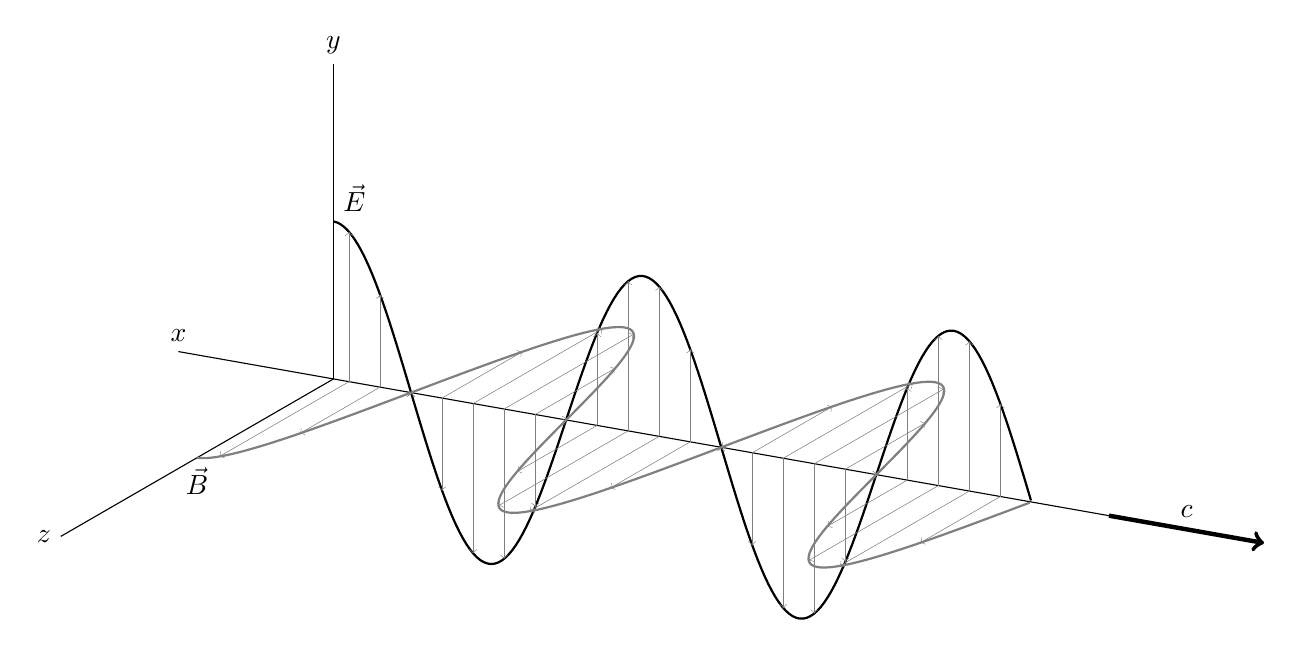
\begin{tikzpicture}[scale=2,x={(-10:1cm)},y={(90:1cm)},z={(210:1cm)}]
		    % Axes
		    \draw (-1,0,0) node[above] {$x$} -- (5,0,0);
		    \draw (0,0,0) -- (0,2,0) node[above] {$y$};
		    \draw (0,0,0) -- (0,0,2) node[left] {$z$};
		    % Propagation
		    \draw[->,ultra thick] (5,0,0) -- node[above] {$c$} (6,0,0);
		    % Waves
		    \draw[thick] plot[domain=0:4.5,samples=200] (\x,{cos(deg(pi*\x))},0);
		    \draw[gray,thick] plot[domain=0:4.5,samples=200] (\x,0,{cos(deg(pi*\x))});
		    % Arrows
		    \foreach \x in {0.1,0.3,...,4.4} {
		      \draw[->,help lines] (\x,0,0) -- (\x,{cos(deg(pi*\x))},0);
		      \draw[->,help lines] (\x,0,0) -- (\x,0,{cos(deg(pi*\x))});
		    }
		    % Labels
		    \node[above right] at (0,1,0) {$\vec{E}$};
		    \node[below] at (0,0,1) {$\vec{B}$};
		  \end{tikzpicture}
		
		  \begin{minipage}{.5\linewidth}
		    \[
		      c = \frac{E}{B}
		    \]
		    \begin{tabular}{r@{${}={}$}p{.8\linewidth}}
		      $\vec{E}$ & electric field amplitude \\
		      $\vec{B}$ & magnetic field amplitude (instantaneous values) \\
		      $c$ & speed of light ($3\times10^8\mathrm{m/s}$) \\
		    \end{tabular}
		  \end{minipage}%
		  \begin{minipage}{.5\linewidth}
		    \[
		      c = \frac{1}{\sqrt{\mu_0 \varepsilon_0}}
		    \]
		    \begin{tabular}{r@{${}={}$}p{.8\linewidth}}
		      $\mu_0$ & magnetic permeability in a vacuum, $\mu_0 = 1.3\times10^{-6}\,\mathrm{N/A^2}$ \\
		      $\varepsilon_0$ & electric permeability in a vacuum, $\varepsilon_0 = 8.9\times10^{-12}\,\mathrm{C^2/N m^2}$ \\
		    \end{tabular}
		  \end{minipage}
	\end{center}

	The propagation velocity of the electromagnetic wave in the a material is then given by:
	
	We have $v<c$ because experience has show so far that we can not exceed the speed of light, which is one of the postulates of Special and General Relativity.

	So we can finally write:
	
	Therefore using the d'Alembertian in one dimension:
	
	As we failed to get a direct expression of $E(x, t)$ and $B (x, t)$, we have just obtained differential equations containing only one of these fields. We name these equations respectively "\NewTerm{wave equation for the electric field}\index{wave equation for the electric field}" and "\NewTerm{wave equation for the magnetic field of induction}\index{wave equation for the magnetic field of induction}".

	The both equations have the same form and admit a solution of the same type. An obvious and particular solution (we leave it to the reader to make this check) of these differential equations is the sine trigonometric function:
	
	by not forgetting the relation between the pulsation $\omega$, the propagation velocity $c$ and the wave number $k$ that we had proved in the section of Wave Mechanics!

	A more general solution is the sum of the trivial solutions (\SeeChapter{see section Differential and Integral Calculus page \pageref{sum solutions of differential equations}}):
	
	But we have seen in our study of phasors (\SeeChapter{see section Wave Mechanics page \pageref{phasors}}) that this real solution is only a particular case of a more general solution that is in the imaginary number field. So finally we can write:
	
	Which constitutes the "\NewTerm{monochromatic plane wave}\index{monochromatic plane wave}\label{monochromatic plane wave}" which is the simplest type of wave to manipulate in physics.

	In three dimensions, the solution is by extension:
	
	where $\vec{k}$ is named the "\NewTerm{propagation vector}\index{propagation vector}".
	\begin{tcolorbox}[title=Remark,colframe=black,arc=10pt]
	The monochromatic wave can has no real signification as physical reality. Indeed, if we calculate the electrical energy associated with in all space, we obtain for it an infinite energy (as it has neither beginning nor end!) Which is not realistic. We will see in the section of Wave Quantum Physics that in fact the light is enclosed in a quantum of energy.
	\end{tcolorbox}
	But the wave equation is linear (solution is always the sum of other solutions). This implies that a superposition of waves of different frequencies (wave number and pulsation also!) is also a solution. Thus, by varying the wave vector $\vec{k}$ (and implicitly via its norm $||\vec{k}||$, pulsation $\omega$, frequency $f$ and period $T$) we also scan all the possible directions of propagation.

	Written mathematically this gives, for the electric field:
	
	And nothing prevents us from extracting a coefficient of the initial amplitude of the field such that:
	
	and we find here a relation very similar to that of an inverse Fourier transform (\SeeChapter{see section Sequences and Series page \pageref{fourier transform}}) which is a remarkable fact! So the trick is now to put $t=0$ because the previous relation is not just a simple analogy with the Fourier transform, it is a Fourier transform!!!!

	We can therefore relate the real field $\vec{E}(\vec{r},0)$ to the field $\vec{E}_0(\vec{k})$:
	
	These two relations are often condensed as following:
	
	The real field is thus at the initial instant the inverse Fourier transform of the field $\vec{E}_0(\vec{k})$. The term $\vec{E}_0(\vec{k})$ therefore represents the spectral component related to the particular wave vector $\vec{k}$ of the real field. This general solution of the wave equation is named "\NewTerm{wave packet}\index{wave packet}"
	\begin{tcolorbox}[title=Remarks,colframe=black,arc=10pt]
	\textbf{R1.} Identically to our study of Wave Mechanics the coefficients $\omega$ (pulsation) and $\vec{k}$ (wave number) coefficients are required to express the variation of the sine by radians and to give it a direction and a pulsation (\SeeChapter{see section Wave Mechanics page \pageref{wave number}}).\\

	\textbf{R2.} The periodicity of the sine function requires (\SeeChapter{see section Trigonometry page \pageref{trigonometric circle}}):
	
	hence the definition of the period of a wave:
	\\

	\textbf{R3.} The periodicity in space makes it possible to define identically the wavelength of the function as:
	
	We thus observe that the plane wave moves along $x$ by traveling a distance $\lambda$ in a time $T$. The velocity of the electromagnetic wave is then:
	
	\end{tcolorbox}
	By introducing:
	
	Into the one dimensional version of:
	
	we get:
	
	to finally obtain the famous result for the plane electromagnetic wave:
	
	
	\subsubsection{Helmholtz equation}
	Now let us examine in detail another solution of the form:
	
	where this time we make explicit mention of the coordinates in order to avoid any confusion.
	\begin{tcolorbox}[title=Remark,colframe=black,arc=10pt]
	The particular solution with the cosine is more appreciated by many teachers than the one with the sine, as it allows, as we will see, a condensed writing using the phasors (\SeeChapter{see section Wave Mechanics page \pageref{phasors}}).
	\end{tcolorbox}
	If we use the concept of phasor, we can rewrite this solution in the form:
	
	Therefore:
	
	into the wave equation:
	
	we get:
	
	which is nothing else that one the "\NewTerm{one-dimensional Helmholtz equation for electrodynamics}\index{Helmholtz equation for electrodynamics}". It is just a special way to write the conventional Helmholtz that is traditional in this field of physics.

	More generally in undergraduate courses it is defined using the prior previous wave equation and rearranging it as following:
	
	and using the property established earlier above:
	
	But we can write it for the three dimension case also:
	
	And using the laplacian operator (\SeeChapter{see section Vector Calculus page \pageref{laplacian of vector fields}}):
	
	Factorized:
	
	And as it is also valid for the magnetif field we can generalize the notation a last time:
	
	to get the "\NewTerm{homogeneous wave equation}\index{homogeneous wave equation}" (as the second term is zero).

	This done, separation of variables (\SeeChapter{see section Differential and Integral Calculus page \pageref{separation vaiables method}}) begins by assuming that the wave function $f(\vec{r}, t)$ is in fact separable:
	
	Substituting this form into the homogeneous wave equation, and then simplifying, we get immediately the following equation:
	
	Notice the expression on the left-hand side depends only on $\vec{r}$, whereas the right-hand expression depends only on $t$. As a result, this equation is valid in the general case if and only if both sides of the equation are equal to a constant value that we will denote by $C$. From this observation, we obtain two equations, one for $A(\vec{r})$, the other for $T(t)$:
	
	Rearranging the first equation, we get the famous "\NewTerm{general homogeneous Helmholtz equation}:
	
	and this is the common general "\NewTerm{Helmholtz equation}\index{Helmholtz equation}" partial differential equation.
	\begin{tcolorbox}[title=Remark,colframe=black,arc=10pt]
	If in the Helmholtz equation we put $C=0$ we get:
	
	More commonly denoted:
	
	and named the "\NewTerm{Laplace's equation}index{Laplace's equation}". It is therefore a special case of the Poisson's equation but where the second member is equal to zero.
	\end{tcolorbox}
	
	
	\subsubsection{Energy flow transportation (Poynting vector)}\label{poynting vector}
	It is relatively intuitive that any electromagnetic wave must carry energy. Let us express the value of this energy in a classical (non-probabilistic and non-quantic) point of view.

	Since the propagation direction of an electromagnetic wave is that of the vector $\vec{E}\times\vec{B}$ as proven earlier above, we can define the "\NewTerm{Poynting vector}\index{Poynting vector}" as:
	
	named sometimes the "\NewTerm{Abraham form}\index{Abraham form}" andhose value is expressed indeed in joules per second and per unit area (radiated power by surface unit) as $[\text{J}\cdot\text{s}^{-1}\cdot\text{m}^{-2}]$.

	The norm of the Poynting vector represents therefor the instantaneous power which is transported by the electromagnetic wave through a unitary perpendicular surface (we insist on the "perpendicular") to its direction of propagation. Therefore, we can also write the Poynting vector in the following form (be careful not to confuse the energy and the electric field which are represented by the same letter):
	
	where $\vec{n}$ is as usual the unit vector perpendicular to $\mathrm{d}S$ (this last relation will be useful to study a small property of the synchrotron radiation further below).

	For a plane electromagnetic wave, the norm of the Poynting vector is:
	
	This quantities varies according to time and place. At a given location, its average value is the mean value of the $sin^2(\ldots)$ for a period $T$:
	
	Let us recall that (\SeeChapter{see section Differential and Integral Calculus page \pageref{usual primitives}}):
	
	Therefore $\forall x$ we have:
	
	The average value of the Poynting vector of a plane electromagnetic wave is a constant ... which does not depend on position and time.
	
	\begin{tcolorbox}[title=Remark,colframe=black,arc=10pt]
	We can make a daring and fun analogy with electrokinetics by doing a dimensional analysis of the above product $\mu_0c$. We have:
	
	\end{tcolorbox}
	... to demonstrate the energy contained in a unit of volume pragmatic physicists would do a dimensional analysis. Let us avoid this and focus ourselves with the special case of the plane wave!

	For this purpose we base ourselves on the electrical energy of an ideal plane capacitor (\SeeChapter{see section Electrostatics page \pageref{capacitor}}) producing plane electromagnetic waves with a yield of $100\%$:
	
	Therefore:
	
	and that is denoted in most textbooks by:
	
	from which we get:
	
	And the total energy transported by the electromagnetic wave in this particular case is thus:
	
	Therefore, the electrical energy density of an electromagnetic wave is equal to its magnetic energy density.

	From this result, we are led to define the "\NewTerm{mean intensity $I$ of an electromagnetic wave}" by the average value of its Pointing vector:
	
	It is therefore the average power that carries the wave per unit area. We have already demonstrated the mean expression of the Poynting vector, which leads us to write:
	
	Now, using the relation between energy and linear momentum (\SeeChapter{see section Special Relativity page \pageref{relativistic mass momentum relation}}):
	
	we get the "\NewTerm{linear momentum density}\index{linear moment density}" of the electromagnetic wave:
	
	But if the direction of $\vec{E}\times\vec{B} $ is perpendicular to the wavefront and is therefore confounded with the propagation direction of the wave its module is:
	
	We therefore have for the linear momentum density:
	
	As the linear momentum density must have the direction of propagation, we can write it in vector form:
	
	If an electromagnetic wave has a linear momentum density, it also has a kinetic angular momentum. The angular momentum per unit volume is then:
	
	Thus, an electromagnetic wave carries both linear momentum density and angular momentum density as well as energy density !!!

	This result is not surprising. Electromagnetic interaction between two electrical charges involves an exchange of energy and momentum between loads. This is done through the electromagnetic field which carries a density of energy and momentum density that are exchanged.
		
	\pagebreak
	\subsubsection{Emissions}\label{electromagnetic emissions}
	To predict the shape and properties of the radiation emitted by antennas or other sources, computers and numerical models corresponding to the problem to be studied should be rigorously used. Formally, solving Maxwell's equations in macroscopic systems is quite difficult and takes time. Moreover, this is rather the work of the engineer who seeks practical exploitation from fundamental theories. The theoretical physicist is interested in the foundations of the Universe and with isolated and perfect systems.

	However, we would like to expose the theory of diffraction and for this we must make a theoretical trip on an approximation of the properties of the radiation of a spherical point source in the vacuum.

	The wave in the case of a spherical point source propagates spherically in space (we speak then of "\NewTerm{spherical wave}\index{spherical wave}\label{spherical wave}") and the Poynting vector of is therefore obviously radial to the source.
	\begin{figure}[H]
		\centering
		\includegraphics[scale=0.47]{img/electromagnetism/spherical_wave_front.jpg}
		\caption[Spherical wavefront]{Spherical wavefront (source: ?)}
	\end{figure}
	The vector $\vec{E}(r,t)$ and $\vec{B}(r,t)$ and vectors are locally contained in the plane tangent to the sphere of radius $r$ (logical!) as shown in the figure below:
	\begin{figure}[H]
		\centering
		\includegraphics{img/electromagnetism/spherical_wave_poynting_vector.jpg}
		\caption[]{Representation of the propagation with respect to the plane tangent to the sphere}
	\end{figure}
	For the flow energy to be constant, the intensity of the wave must decrease with distance. Indeed, the conservation of the energy imposes that through a sphere of radius $r_1$ the energy radiated per unit of time (written with an right "E" so as not to be confused with the notation of the electric field) is equal to that which traverses the sphere of radius $r_2$:
	
	This naturally implies:
	
	But using the relation proved earlier above:
	
	and using the property of perpendicularity of the electric and magnetic field for a plane wave:
	
	Therefore:
	
	which implies:
	
	that is to say:
	
	and therefore the magnitude of the electric or magnetic of a electromagnetic plane wave field decrease inversely proportional to the distance $r$:
	
	Thus the intensity density $I$ of a spherical electromagnetic wave propagating in the vacuum decreases in $r^2$ since:
	
	Therefore:
	
	By extension (important information for mobile phones and radio communications), in view of the results demonstrated above, the energy transported thus decreases in also in $1/r^2$.
	
	It is now easy to understand now why physicists systematically use the frequency to characterize a electromagnetic wave because its amplitude is not constant in the vacuum whereas the frequency is a kind of signature of the transmitter that is not lost through a static empty space !!!
	
	\pagebreak
\	\subsection{Synchrotron radiation (bremsstrahlung)}\label{bremsstrahlung}
	Broadly speaking, "\NewTerm{Bremsstrahlung}\index{Bremsstrahlung}" or "\NewTerm{braking radiation}\index{braking radiation}" is any radiation produced due to the deceleration (negative acceleration) of a charged particle, which includes synchrotron radiation, cyclotron radiation, and the emission of electrons and positrons during beta decay. However, the term is frequently used in the more narrow sense of radiation from electrons (from whatever source) slowing in matter.
	
	A synchrotron light source is a source of electromagnetic radiation (EM) usually produced by a storage ring or more generally any electric charge particle in acceleration. First observed in synchrotrons, synchrotron light is now produced by storage rings and other specialized particle accelerators, typically accelerating electrons. Once the high-energy electron beam has been generated, it is directed into auxiliary components such as bending magnets and insertion devices (ondulators or wigglers) in storage rings and free electron lasers. These supply the strong magnetic fields perpendicular to the beam which are needed to convert high energy electrons into photons.
	\begin{figure}[H]
		\centering
		\includegraphics[scale=0.25]{img/electromagnetism/synchrotron.jpg}
		\caption[European Synchrotron]{European Synchrotron (source: ESRF)}
	\end{figure}
	The major applications of synchrotron light are in condensed matter physics, materials science, biology and medicine. A large fraction of experiments using synchrotron light involve probing the structure of matter from the sub-nanometer level of electronic structure to the micrometer and millimeter level important in medical imaging. An example of a practical industrial application is the manufacturing of microstructures by the LIGA process.
	\begin{figure}[H]
		\centering
		\includegraphics[scale=1]{img/electromagnetism/synchrotron_source.jpg}
		\caption[Synchrotron source produces electromagnetic radiation]{Synchrotron source produces electromagnetic radiation, as evident from the visible glow (source: United States Department of Energy)}
	\end{figure}
	It is also an important subject of study because the Rutherford  Model (\SeeChapter{see section Corpuscular Quantum Physics page \pageref{rhuterford model}}) was a not able to explain the fact that there was not Bremsstrahlung of the electron orbiting around the nucleus as at it's time the Bremsstrahlung was a well known effect!
	
	To begin, let us consider an electric charge in uniform rectilinear motion. The electrical and magnetic fields of such an electric charve have been studied in the previous sections. We have also shown above that the magnetic field is in this configuration, always perpendicular to the electric field. The first consequence is that the electric field is radial and the magnetic field transverse.

	So if we surround the moving particle of an imaginary closed spherical surface, we then have trivially (see the definition of the Poynting vector):
	
	since at any point on the surface, $\vec{E}$ is perpendicular to it and $\vec{B}$ tangent to it, hence $\vec{E}\times\vec{B}$ is also tangent to the surface and therefore the angle between $\vec{E}\times\vec{B}$ and $\vec{n}$ is equal to a right angle therefore the scalar product is zero.

	Thus, in conclusion, the total flux of radiated energy is zero for an electric charge in uniform rectilinear motion. In other words, a uniformly rectilinear moving electric charge does not radiate electromagnetic energy but carries with it the energy of the electromagnetic field (here we are reassured!). This is confirmed by the experimental observations.

	However, the situation is very different for an accelerated moving electric charge. The electric field of an accelerated charge is no longer radial and no longer possesses the symmetry with respect to the charge which it possesses when the motion is uniform (as will we prove it). Consequence: ... an accelerated electric charge radiates electromagnetic energy and therefore sees its kinetic energy that decrease!

	An important conclusion is that in order to maintain an electric charge in accelerated motion, it is necessary to provide energy to compensate for that lost by radiation. If the particle instead of being accelerated is decelerated (it is typically what we seek to do in radioprotection) again the particle will emit the same radiation in the same way (we will also prove it). This happens, for example, when an electric charge, such as an electron or a proton, strikes a target at high speed. A substantial fraction of its total energy goes in the form of a radiation.

	The equations that we are going to determine remain valid for any type of relativistic accelerated motion or not (but not from a quantic point of view!). For example, a charged particle moving in a circular orbit is subjected to centripetal acceleration and therefore emits radiation. Consequently, when an ion is accelerated in a cyclic accelerator such as a cyclotron, betatron or synchrotron, a fraction of the energy supplied to it is lost as electromagnetic radiation. Cyclic accelerators than in linear accelerators.
	
	When the electric charges reach very high energies, as it happens in synchrotrons where the acceleration is great (fortunately for us because it will allow us to make a very useful approximation ...), the losses due to radiation, named "synchrotron radiation" as we already know, become important and constitute a serious limitation in the construction of cyclic accelerators of very high energy but nevertheless remain infinitely useful to the advanced industry and scientific medicine and archeology.

	Another important consideration relates to the atomic structure. According to the atomic model of Rutherford (\SeeChapter{see section Corpuscular Quantum Physics page \pageref{rhuterford model}}), we imagine the atom as formed of a positively charged central nucleus, the negatively charged electrons describing closed orbits around it. But this implies that the electrons move with accelerated motion and, if we apply the ideas developed so far, all atoms should continuously radiate energy (even in the absence of an external source of energy like the Sun). As a result of this loss of energy, electronic orbits should contract, resulting in a corresponding reduction in the size of all bodies. Fortunately for us, this is not observable (matter does not collapse on itself), but this leads us to suppose, within the framework of the Rutherford model, that the movements of electrons in atoms are governed by certain principles which were not considered at its time. This is what will lead us to create the Bohr model of the atom (\SeeChapter{see section Corpuscular Quantum Physics page \pageref{bohr model}}) but which, as we shall see, will also have other defects.

	To determine the energy emitted by an electric charge in accelerated motion we will have to make use of mathematical tools that are no longer at the same level as those used previously. It is therefore recommended that the reader have a good mathematical background. Moreover, exceptionally we will make use of CAD softwares for certain points of the development.

	Let us consider first the following figure:
	\begin{figure}[H]
		\centering
		\includegraphics[scale=1]{img/electromagnetism/synchrotron_study_configuration.jpg}
		\caption[]{Scenario to consider for the study of synchrotron radiation}
	\end{figure}
	When the charge distribution $\rho(\vec{r},t')$ and the current distribution $\vec{J}(\vec{r},t')$ are at the point $P_2$, the point $M$ receives the electromagnetic wave emitted by the electric charges and the current when they were at the point $P_1$, ie at the instant $t'$ (because of the speed limit $c$ of the propagation of the field in space). The time delay is the propagation time from the point $P_1$ to the point $M$, ie:
	
	Therefore:
	
	Therefore:
		
	The scalar and vectorial potentials associated respectively with the electric field and the magnetic field at the point of vectorial coordinate $\vec{R}$ at time $t$ have, on the basis of the results obtained in the two preceding sections, the following expressions:
	
	where on the other hand we have to prove imediately in detail that the vector potential associated with the magnetic field is expressed as indicated above!
	\begin{tcolorbox}[title=Remark,colframe=black,arc=10pt]
	We will use these two relations of potential in our study of the radiated field because their similar mathematical form will allow us, at least we hope it..., to simplify the developments.
	\end{tcolorbox}
	These two relations are already partially familiar to us, the first one expressing the (delayed) electrical potential has been proved in the section of Electrostatics in the non-relativistic framework (so our calculations may not be correct if we come across a result that depends on the speed! We will see...).

	Concerning the second relation which expresses the delayed potential-vector, we have seen above that:
	
	was always correct to given gradient of an additive function for $\vec{A}$ (due to the properties of the differential vector operators) such that:
	
	and that $\vec{B}$ is in relativistic form or not, we have:
	
	Let us also recall that we have the Biot-Savart law (\SeeChapter{see section Magnetostatics page \pageref{biot savart law}}) that:
	
	It follows that if we put:
	
	we fall back on the Biot-Savart law since if and only if $\vec{J}$ does not depend on $r$ then (trivial):
	
	We thus get indeed:
	
	Although this form of vector potential gives only the Biot-Savart's law in non-relativistic form, as still always satisfies:
	
	this is still valid in the relativistic framework because this Maxwell equation does not depend on the velocity. Moreover, if our results in the study of synchrotron radiation give us at the end an expression independent of velocity, we shall have once again confirmed this fact.

	\subsubsection{Liénard-Wiechert potentials}\label{linear wiechard potentials}
	Liénard–Wiechert potentials describe the classical electromagnetic effect of a moving electric point charge in terms of a vector potential and a scalar potential in the Lorenz gauge. Built directly from Maxwell's equations, these potentials describe the complete, relativistically correct, time-varying electromagnetic field for a point charge in arbitrary motion, but are not corrected for quantum-mechanical effects. Electromagnetic radiation in the form of waves can be obtained from these potentials. These expressions were developed in part by Alfred-Marie Liénard in 1898 and independently by Emil Wiechert in 1900.
	
	To start this study, let us consider the case where a particle of mass $m$ and of electric charge $q$ travel a path $\Gamma$. Compared to an origin point O, its vector coordinate is $\overrightarrow{\text{O}P}=h(t)$, its velocity vector will be denoted:
	
	and its acceleration:
	
	If the point charge $q$ is at the origin O, we saw in the section of Differential and Integral Calculus that the Dirac function gives us:
	
	and if the punctual electric charge $q$ is at an abscissa $x_0$, we have:
	
	What has just been said for a one-dimensional space can also be applied to a three-dimensional space as we saw it and then we write:
	
	If we choose inverse cubic meters ($[\text{m}^{-3}]$) for units for the Dirac function, then we can write:
	
	where $q$ is then the total charge at the point $\vec{r}$.

	For the distribution of the current density, we also have also by choosing the same units as for the Dirac function:
	
	Therefore, at point $M$, the potentials at time $t$ have for expression:
	
	This is a very useful formulation (a workaround) that will enable us to solve our problem.

	For this purpose, when the electric charge is at the point $P_1$ at the time $t'$, we put:
	
	We will use a looooong artifice to solve the integral of the electrical potential (which is therefore an integral multiple in Cartesian coordinates)!

	This begins by multiplying the factor under the integrand $U(\vec{R},t)$ by:
	
	this does not modify the integral since:
	
	and that (\SeeChapter{see section Functional Analysis page \pageref{dirac function}}):
	
	We then have the following expression in which the time $t'$ appears:
	
	what we have the right to write because the second integral does not depend explicitly on $t'$.
	
	Good now if we try to solve this integral, we will spend our lives on it... for nothing. We'll have to be more clever!

	Before looking for a solution of this integral, we must first deal with the more general case of the following integral:
	
	Or written in a more condensed form:
	
	which it is easy to approximate with the prior-previous integral:
	
	where we have deal such that $f_1,f_2,f_3,f_4$ depend respectively only (explicitly) on $x$, $y$, $z$ and $t'$ 

	We now want now to make the following change of variables:
	
	Let us recall that in changes of variables in multiple integrals (see the Jacobian in the section of Differential and Integral Calculus), we have, passing from Cartesian coordinates to curvilinear coordinates, the following relations:
	
	where for recall:
	
	and where:
	
	is not an absolute value but the determinant of a matrix!
	
	Now, in our case, let us recall that we have all the $f_i$ which are null and therefore:
	
	and in the case where during the developments one of the $f_i$ would no longer be zero for reasons not yet determined, we would have:
	
	The multiple integral then becomes:
	
	Where the term between braces is taken at $f_i=0$ by necessity of the construction of previous developments preparing the mathematical artifice!

	And let us recall once more (!!) the property of Dirac functions:
	
 	We then have immediately the simplification:
	
	where:
	
	is therefore the Jacobian of the transformation of the artifice ...

	It is evident that by construction of the Jacobian we have:
	
	Therefore it comes:
	
	For the integral $I$ we then have:
	
	Let us now calculate our Jacobian ...:
	
	Returning to the our treated case, $\vec{R}-\vec{h}(t')$ therefore has for components:
	
	Therefore, we have the calculation of the elements of the inverse of the Jacobian:
	
	Well... now that we have the components of the Jacobian matrix, we have only to calculate its determinant. So either we use the general relation of the calculus of determinant proved in the section of Linear Algebra, or we use Maple ... So to win a little bit time let's do it with Maple 4.00b:
	
	\texttt{>with(linalg):\\
	>A:=matrix(4,4,[1,0,0,a,0,1,0,b,0,0,1,c,d,e,f,1]);}
	
	where (for people having difficulty to read Maple notations):
	
	with:
	
	Let us continue with Maple 4.00b:

	\texttt{>Det (A);}
	
	Which gives as output:

	\begin{center}
		\texttt{1 - cf - eb - da = 1 - (fc + eb + da)}
	\end{center}
	The inverse of the Jacobian has the for expression:
	
	Where we used the dot product in the prior-previous equality in order to condense the expression.

	Therefore:
	
	The multiple integral:
	
	where for recall:
	
	or written differently:
	
	But as a result of our change of coordinate system we have for recall:	
	
	And let us recall once again that:
		
	Therefore we have to take $g$ on $f_1=f_2=f_3=f_4=0$! It comes:
	
	Which allows to write:
	
	It is same for:
	
	that can then be written as:
	
	Finally, the resolution of the integral $I$ is written:
	
	Finally, we get the expressions of the potentials.
	\begin{itemize}
		\item The scalar potential is then written:
		

		\item The vector potential is written:
		
		Considering that the integral which is almost the same as for the scalar potential except the term $\vec{v}'$, we arrive by making the same developments as before with to the expression (please... don't ask us for to put also the details for this one... plzzzzz!):
	
	\end{itemize}
	In summary, the potentials taken at the moment (time delay of propagation):
	
	have for expression in a very condensed form ($K_e$ in the Coulomb constant for recall as introduced in the section of Electrostatics!):
	
	These potentials are named "\NewTerm{Liénard-Wiechert retarted potentials}\index{Liénard-Wiechert retarted potentials}" with:
	
	
	\subsubsection{Retarded Electric and Magnetic fields}
	\StickyNote[2.5cm]{\LARGE To finish translate before year 2020}[6.5cm]
	
	
	
	
	
	
	
	
	
	
	
	
	
	
	
	
	
	
	
	
	
	
	
	
	
	
	
	
	
	
	
	
	
	
	
	
	
	
	
	
	
	
	
	
	
	
	
	
	
	
	
	
	
	
	
	
	
	
	
	
	
	
	
	
	
	
	
	
	
	
	
	
	
	
	
	
	
	
	
	
	
	
	
	
	
	
	
	
	
	
	
	
	
	
	
	
	
	
	
	
	
	
	
	
	
	
	
	
	
	
	
	
	
	
	
	
	
	
	
	
	
	
	
	
	
	
	
	
	
	
	
	
	
	
	
	
	
	
	
	
	
	
	
	
	
	
	
	
	
	
	
	
	
	
	
	
	
	
	
	
	
	
	
	
	
	
	
	
	
	
	
	
	
	
	
	
	
	
	
	
	
	
	
	
	
	
	
	
	
	
	
	
	
	
	
	Anyway, that's a lot of words and not much to look at, so how about some soothing animations? 
	
	Here is a Macromedia Flash animation illustrating the effect (need Adobe Reader to be played) made with MATLAB™:
	\begin{figure}[H]
		\includemedia[activate=pageopen,width=\textwidth,height=500pt,
	]{}{swf/Synchrotron_radiation_gamma1.swf}
		\caption[Synchrotron radiation of a circle moving particle with $\gamma=1.2$]{Synchrotron radiation of a circle moving particle with $\gamma=1.2$ (author: Jason Cole)}
	\end{figure}
	The top left represents the Poynting flux $S$, or the radiation which would be observed. The retarded time is plotted beneath, and the two components of the electric field are plotted on the right. You can see how the retarded time is trailing the particle, and spreads out in a circle at the speed of light.

	We can turn up the energy a bit, now $\gamma = 5$:
	\begin{figure}[H]
		\includemedia[activate=pageopen,width=\textwidth,height=500pt,
	]{}{swf/Synchrotron_radiation_gamma5.swf}
		\caption[Synchrotron radiation of a circle moving particle with $\gamma=5$]{Synchrotron radiation of a circle moving particle with $\gamma=5$ (author: Jason Cole)}
	\end{figure}
	Here the electron is much closer to the speed of light, and is consequently chasing it's own lightcone – notice how there is a much larger jump in retarded time (from yellow to green). This causes the Poynting flux to be squeezed into a smaller time window, it's much more compressed, intense, and energetic. The temporal shortening of the radiation pulse corresponds to a broad bandwidth, and it is precisely this pulse of radiation that corresponds to broadband synchrotron radiation.
	
	What about something less extreme, an electron traveling at constant velocity in a straight line, again at $\gamma = 1.2$:
	\begin{figure}[H]
		\includemedia[activate=pageopen,width=\textwidth,height=500pt,
	]{}{swf/Synchrotron_radiation_gamma_linear.swf}
		\caption[Synchrotron radiation of a uniform moving particle with $\gamma=1.2$]{Synchrotron radiation of a uniform moving particle with $\gamma=1.2$ (author: Jason Cole)}
	\end{figure}
	We now see that the field is being dragged along with the particle, but otherwise not radiating. Because the electron is traveling significantly slower than the speed of light, the field looks relatively undistorted. If you squint you'll notice that the transverse field $E_y$ is stronger than the longitudinal field, which is a manifestation of special relativity (Lorentz transforming a uniform field back into the lab frame where the charge is moving).

	Back to something more interesting, a simple dipole motion at $\gamma = 1.2$:
	\begin{figure}[H]
		\includemedia[activate=pageopen,width=\textwidth,height=500pt,
	]{}{swf/Synchrotron_radiation_dipole.swf}
		\caption{Synchrotron simple dipole motion with $\gamma=1.2$ (author: Jason Cole)}
	\end{figure}
	We see what we hoped for, oscillating radiation perpendicular to the dipole, and zero far-field radiation parallel to the dipole. In the near-field (close to the dipole), there are electric field components everywhere, but it is clear that these must correspond to non-radiative terms and they die off rapidly.

Finally, let’s turn to a use for this radiation: undulators/wigglers. These are machines which purposefully oscillate an electron bunch to force synchrotron radiation emission, where the electron travels with high velocity in one direction and oscillates in the other:
\begin{figure}[H]
		\includemedia[activate=pageopen,width=\textwidth,height=500pt,
	]{}{swf/Synchrotron_radiation_uniform_oscillating.swf}
		\caption{Synchrotron uniform oscillating moving particle (author: Jason Cole)}
	\end{figure}
	
	Notice that:
	
	as:
	
	can be written:
	
	The killer for CERN is that $E^6$ factor because if we double the energy of a particle, it radiates much more times the equivalent received energy. In the case of electrons, this very quickly becomes such a high power that the accelerator can't accelerate any more – the electrons radiate away their energy quicker than it can be pumped in. For protons of the same energy, because of the $m^6$ factor at the denominator the $E^6$ factor is $10^{19}$ times smaller (as $m_p/m_e\cong 1836$), so radiate much less. This is why the LHC is so big, and uses protons rather than electrons. There are plans to build an even bigger LHC, unimaginatively named the "Very Large Hadron Collider", or to accelerate electrons in a straight line so that they radiate much less energy at the proposed International Linear Collider. Both of these propositions are very expensive though, and very large, so there is much interest in smaller accelerators like plasma accelerators.
	
	We can alsom make appear the influence of the radius of the accelerator. Indeed, starting from:
	
	Remember that we have seen in the section of Classical mechanics that for a uniform circular motion:
	
	Therefore it follows:
	
	Hence:
	
	We therefore understand that the bigger is the radius, the small is the radiated power. This is why linear accelerator (considers as infinite curvature radius) are much more interesting than circular accelerator (but more difficult to build as wee need to found and large enough area to build them...).

	\begin{flushright}
	\begin{tabular}{l c}
	\circled{70} & \pbox{20cm}{\score{4}{5} \\ {\tiny 29 votes,  75.86\%}} 
	\end{tabular} 
	\end{flushright}

	%to force start on odd page
	\newpage
	\thispagestyle{empty}
	\mbox{}		
	\section{Electrokinetics}\label{electrokinetics}
	\lettrine[lines=4]{\color{BrickRed}T}he development of electrodynamics has enabled a part of the humanity to significantly change its life quality. We know almost all today what we have thanks to it: fridge, radio, TV, computers, scanners,  cars, trams, trains, planes, robots, smartphones, tablets, and other wonderful things and also sometimes less wonderful...
	
	Before you start studying electrokinetic (engineers speak of "electronics" or "electrotechnics"), that is to say the structures involving electric charges in movement, we will define the two fundamental laws (the term "law" is a misnomer, as the first one was proved in the section Electrostatics and the second one in the section of Electrodynamics but anyway...) of the study of electrokinetic and the basic terminology/jargon of electrical circuits or equipment (practical cases being studied in section Electrical Engineering). Even if some elements in the beginning of this section will perhaps not immediately be understood by the reader (especially industrial applications), they will become trivial as the progress of reading of the section.
	
	\textbf{Definitions (\#\mydef):}
	\begin{enumerate}
		\item[D1.] An electrical circuit is constituted by a set of devices named "\NewTerm{dipole}\index{dipole}", interconnected by a conductive wire.
		
		\item[D2.] A "\NewTerm{node}\index{node}" of a circuit is an interconnection where three or more conductor wire are connected together.
		
		\item[D3.] A "\NewTerm{branch}\index{branch}" is a circuit section between two nodes.
		
		\item[D4.] Finally, a "\NewTerm{mesh}\index{mesh}" is a set of branches forming a closed loop.
	\end{enumerate}
	\begin{figure}[H]
		\centering
		\includegraphics[scale=0.9]{img/electromagnetism/circuit_vocabulary.jpg}
		\caption{Circuit basic vocabulary}
	\end{figure}
	\begin{tcolorbox}[title=Remark,colframe=black,arc=10pt]
	It is very important to understand what will follow! Some developments will be reused in the section of Special Relativity, Quantum Field Theory, etc. Furthermore, the reader should also read in parallel the section of Special Relativity to better understand the ins and outs of certain results and the provenance of some mathematical tools.
	\end{tcolorbox}
	The dipole is characterized by the response in a current $I$ by (most of time) a difference of electric potential $U$ between its terminals. That is to say i.e. by the characteristic curve:
	
	Obviously some dipoles reacts on radiations difference, or on rotation difference, on pressure, on humidity and son on...
	
	We shall see that in any conductor, the presence of a resistivity (see below the concept) causes a voltage drop and, strictly speaking, it is the same for the wires (made of conductor material). But these latter being connected in series with other dipoles, we neglect usually in small circuits the resistance of wires relatively to those of the dipoles. Therefore, the wires located between two dipoles of a small circuit are supposed to be equipotentials (the potential is the same on the two terminals).
	
	\subsection{Kirchoff's laws}
	If you connect lots of passive or active elements together in a complicated network, then currents will flow through all the various elements so as to insure that charge is conserved, energy is conserved, and Ohm's Law is satisfied for each resistor.
	
	Simultaneously satisfying all these conditions will give you exactly one solution. The method for writing down equations to represent these conservation laws is named "\NewTerm{Kirchhoff's Laws}\index{Kirchhoff's Laws}" (not to be confused with those of the thermodynamics and optics bearing the same name!) and express the physical properties of the charge and the electric field and are at the number of $2$ (one law for each property).
	
	Briefly:
	\begin{enumerate}
		\item The total current flowing towards a node is equal to the total current flowing from that node
		
		\item In a closed circuit, the algebraic sum of the products of the current and the resistance of each part of the circuit is equal to the resultant electromotive force in the circuit. 
	\end{enumerate}
	
	They will enable us without using the heavy mathematical artillery implicitly hidden behind just to get highly relevant results.
	
	\subsubsection{Mesh law (Kirchhoff's Loop Law)}
	The mesh law (implicitly it is simply the conservation of energy) expresses the fact that when a charge browse a closed circuit (closed path), the energy it loses in by browsing a part of the circuit is equal to the energy it gains in the other. Thus, the algebraic sum of the potentials along a mesh is zero such that:
	
	For this, we must arbitrarily choose a direction of travel of the mesh and agree that the tensions whose arrow points in the direction of travel are counted as positive and others as negative.
	\begin{tcolorbox}[title=Remark,colframe=black,arc=10pt]
	This law simply expresses the fact that the electric field (Coulomb) is a conservative vector field as we have seen in the section of Electrostatic.
	\end{tcolorbox}
	
	\subsubsection{Nodes law (Kirchhoff's Point Law)}
	The nodes law (implicitly it is simply the current conservation law) expresses the conservation of charge, which means that the sum of currents leaving a node (a node can be seen as a separator of field lines - in extenso volumes connected by a same surface) is equal to the sum of currents entering the node. In other words, the algebraic sum of the currents is zero at every node of a circuit such that:
	
	For this, we must choose a sign for incoming currents and the opposite sign for outgoing currents (as we do in Thermodynamics with the mass).
	\begin{tcolorbox}[title=Remark,colframe=black,arc=10pt]
	This law simply expresses the charge conservation equation (or equivalently the law continuity of the charge) that we have proved in the section Electrodynamics.
	\end{tcolorbox}
	\begin{figure}[H]
		\centering
		\includegraphics[scale=0.5]{img/electromagnetism/apply_kirchhoffs_law.jpg}
		\caption[]{Try to apply Kirchoff's law...}
	\end{figure}
	
	\subsection{Drude model}
	The Drude model of electrical conduction will allow us to introduce the basic concepts of the electrokinetic. First, let us define inf what will follow the concept of "\NewTerm{Electric Current}\index{electric current}", "\NewTerm{electric current density}\index{electric current density}", and "\NewTerm{electric resistance}\index{electric resistance}".
	
	An electrical conductor (we are not talking about semiconductors and superconductors at this level of our discussion) can be seen in a very simplified way as a pipe section $\vec{S}$ containing an electron gas of $n$ elementary electric charges $q$ per unit volume.
	
	In the absence of electric field, each electron has a zero vector average speed because it remains in the vicinity of the atom. Under the action of a constant and homogeneous electric field $\vec{E}$ (the case of direct current therefore!), some electrons are moved in a particular direction, until they collide with another atom (traditional aspect... not quantume one obviously!!!) where they take again an average vectorial zero speed drift and so on.
	
	This is the oldest model and the most basic one of the electric current. The bases were laid by Paul Drude in 1902, shortly after the discovery of the electron by Joseph John Thomson (1897). Hence the name "\NewTerm{Drude model}\index{Drude model}".
	
	Insufficient to conceive and develop most of the active electrical components that exists since the late 20th century, the billiard balls model has nevertheless considerable interests:
	
	\begin{itemize}
		\item This is a useful tool to give to our limited mind a picture of phenomena we do not get any direct perception (at least at this day), since they take place in the infinitesimal world of atomes an elementary particles.

		\item The results, for the engineer, of more accurate modern theories, especially such as energy band theory, allow themselves to be formulated using the same concepts as those appearing in the "Billiard Balls" Drude model. Let us quote among them the "density number" and the "electron mobility" concepts (that we will introduce later rigorously further below in our study of energy band theory).

		\item Even if this approach is quite primitive, this model leads to a phenomenological interesting interpretation of the fundamental laws such as Ohm's law or the Joule's law. It binds together certain microscopic phenomena and observable quantities.
	\end{itemize}
	As it's friendly name suggests it, this model treats the electrons as tiny billiard balls. These particles are therefore considered as classical objects, simply governed by Newton's and Maxwell's laws proved in previous sections of this book. This corpuscular conception of the electron is also not totally opposed to the results of quantum physics (study in the next sections of this book), in which a wave packet can always be interpreted as a particle with its mass and speed (see the Ehrenfest's theorem in the section of Wave Quantum Physics).
	
	In a millimeter copper cube, we assume that the number of electrons is so high that it therefore does not matter then treat individually, which would also be irrelevant. It is the average behavior of electrons that should be studied! Two types of interactions that determine behavior are:
	
	\begin{itemize}
		\item The interaction of electrons with the material in which they operate, and to which they belong;
	
		\item The interaction of electrons with the electromagnetic field applied from the outside (all other interaction being neglected).
	\end{itemize}
	The distance $\lambda$ traveled by an electron distance is named "\NewTerm{electron mean free conduction path}\index{electron mean free conduction path}" and if $\tau$ is the time interval between two successive collisions then we have trivially:
	
	whe $v$ is obviously the mean electron velocity of the material.
	
	The collision time is a random variable. All physical parameters maintained as constant, this random variable is stationary, its average value is named "\NewTerm{mean collision time}\index{mean collision time}".
	
	We suppose that:
	
	the mean velocity, is therefore created by the acceleration of the electric field (\SeeChapter{see section Electrostatic page \pageref{electric force}}):
	
	We then get the "\NewTerm{mean drift velocity}\index{mean drift velocity}" or simply electrons "\NewTerm{drift velocity}\index{drift velocity}" given by:
	
	This relation is so named because their initial speed is maintained due to the thermal excitation of the external environment and corresponds to the thermal velocity for which we have determined the expression in our study of the Maxwell-Boltzmann distribution in the section of Statistical Mechanics (we will calculate their further below in this section).
	
	We admit, in the context of the billiard balls model, that electrons behave like atoms of an ideal gas. This is a gross approximation but enough satisfying for now!
	
	The mean velocity is assumed to be identical for all the free electrons when a constant homogoneous electric field is applied, stationary, and directed along a single axis. It gives the possibility to define the "\NewTerm{current intensity $I$}\index{current intensity}" of electric current in the conductor.
	
	\textbf{Definition (\#\mydef):} The "\NewTerm{electric current}\index{electric current}" or "\NewTerm{electric intensity}\index{electric intensity}", denoted by $I$,  measures the charge $\mathrm{d}Q=nq$ that passes through the cross section $S$ of a conductor per unit of time $\mathrm{d}t$ and is given according to what has been shown just before by:
	
	A slice of conductor, of volume $\mathrm{d}V=S\mathrm{d}L$ contains therefore the electric charge:
	
	It passes through the section $S$ in a time $\mathrm{d}t$, such as:
	
	The current is therefore written:
	
	\begin{tcolorbox}[title=Remark,colframe=black,arc=10pt]
	Attention to the usage of the latter relation in practice! If we consider a theoretical wire, the potential difference across the wire is zero. So there will be no gain / loss of kinetic energy of the electron and therefore no change in speed. If we now consider a real wire, resistive therefore, the potential difference across its terminals will be low but not zero, and the electron's potential drop will not be won in kinetic energy but dissipated as heat in the wire.
	\end{tcolorbox}
	If $I$ is seen as the flow of a "\NewTerm{current density $J$}\index{current density}\label{current density}" through the surface $S$, then we have:
	
	the current density being assumed constant at each point of the surface.
	
	We have therefore:
	
	and after simplification:
	
	which is therefore the expression of the "current density" in the conductor.

	As we know the expression of the velocity, we can write:
	
	And we define the "\NewTerm{conductivity}\index{conductivity}" by:
	
	where this time $n$ is not the number of electrons, but the number density of electrons! By definition, the "\NewTerm{resistance}\index{resistance}" is the inverse of the conductivity!
	
	We notice that the conductivity contains the product of the number density of electron by their mobility. Therefore it is necessary that at least one of these variables has a high value for a material has a high conductivity.
	
	The mobility is greater in the semiconductors than in metals. This characteristic however is completely masked by the ratio of the volumic numbers of electrons: $n$ is between $1,000,000$ to $100,000,000$ times lower in semiconductors than in metals, which explains the higher conductivity of these.
	
	Following the relation:
	
	proved just earlier above, the conductivity depends on the electric field, through the collision time. Indeed, the more the electric field grows, the more the speed of the electrons increases. The distance between the points of possible shocks remaining the same, the collision time, and hence the conductivity should decrease (and thus the resistance increase!).
	
	However, the independence of the conductivity (and respectively the resistance) with the electric field is an experimental fact established precisely with all usual conductors in normal civilian uses.	
	
	The origin of this contradiction lies in the large difference in the magnitudes of the thermal velocity given by the Maxwell-Boltzmann distribution (\SeeChapter{see section Statistical Mechanics page \pageref{maxwell distribution}}):
	
	and of the average speed drift seen above:
	
	with the mean free path time that will be obtained using the expression:
	
	
	We have proved in the section of Statistical Mechanics that for an electron at room temperature:
	
	And let us calculate the drift velocity for copper with for this particular metal the following values:
	
	This allows us to get the value:
	
	and therefore:
	
	Taking $E=0.32 \;[\text{Vm}{}^{-1}]$, which is considered as a high value since this field produces a current density of:
	
	we finally have:
	
	Therefore, even in a strong industrial electric field, the drift velocity is negligible compared to the thermal velocity.
	
	As the thermal velocity depends only a little bit of the electric field, it turns out that in practice the electron velocity is independent of the electric field. In other words, establishing a current, even intense, has only a negligible effect on the speed of electrons!
	
	\begin{tcolorbox}[title=Remark,colframe=black,arc=10pt]
	In the vast majority of cases, the conductor sizes are large, compared to the average distance that an electron travel between two consecutive shocks. The behavior of the surface of the conductive electrons then are of secondary importance. This is why the conductive medium is often implicitly considered as infinite. The FET and MOST transistors  are an important exception to this. The current circulates in a layer thin enough that the electron mobility is affected by electron scattering on surfaces defining this layer.
	\end{tcolorbox}
	However, an important point to notice is the calculation of the mean free path of electrons in the classical Drude model. We have indeed:
	
	which is much higher, at least an order of magnitude (factor of $10$), to the interatomic distances. It results from this that successive collisions with atoms of the network is not responsible for Ohm's law (which we will see now) contrary to one of the initial assumptions of the Drude model but that it are the impurities and defects of the material involved in it that generates the collisions! We will see a further below in the theoretical model of energy bands that the mean free path is in fact still much greater!
	
	Warning!!! This relation may suggest that since the mean free path is proportional to the thermal velocity and therefore proportional to the square root of the temperature, that the resistance decreases with temperature. But in fact it is not so! The Drude model is too simplistic because in reality it is the opposite that occurs for conductors (resistance increases with temperature because the time interval $\tau$ between collisions decreases faster than the speed increases). And then there is also an opposite problem ... almost at a temperature equal to the zero Kelvin (and over for some materials) the mean free path shuld be almost zero but superconductors show us that it is not the case! In short, without explicit relation depending on the temperature we are in total darkness!
	
	The only thing we know how to do is to admit that to a given constant factor $\alpha$ (positive or negative), a temperature change requires a relative change in resistance by (first order Taylor developement):
	
	hence:
	
	The we get the relation know in high-schools:
	
	Finally, let us notice that the fourth Maxwell equation (\SeeChapter{see section Electrodynamics page \pageref{fourth maxwell equation}}) can then be written by  the results obtained just previously:
	
	which then explicitly makes appear the conductivity coefficient.
	
	\pagebreak
	\subsection{Ohm's law}\label{ohm law}
	Ohm's law states that the current through a conductor between two points is directly proportional to the voltage across the two points. Introducing the constant of proportionality, the resistance.
	
	From the relation proved just above:
	
	and taking the definition of "\NewTerm{conductivity}\index{conductivity}" by:
	
	We have finally:
	
	which is the "\NewTerm{local Ohm's law}\index{local Ohm's law}". We have already see it in differential form in the section of Statistical Mechanics and we already know therefore that it belongs in fact to the family of diffusion laws!
	\begin{tcolorbox}[title=Remark,colframe=black,arc=10pt]
	Since the conductivity is necessarily a scalar, the vector notation of Ohm's law implies that the electrostatic field lines also indicate the path taken by the electrical charges. Moreover, as the conductivity is a scalar necessarily positive in the traditional model, this implies that the current has the same direction as the electric field.
	\end{tcolorbox}	
	If we multiply the previous equality under scalar left and right by a length $L$ we get:
	
	Then we have:
	
	or:
	
	We define the inverse of conductivity as the "\NewTerm{electric resistance}\index{electric resistance}" defined by:
	
	\begin{tcolorbox}[title=Remark,colframe=black,arc=10pt]
	It is important to notice that the electrical resistance is proportional to the length of the resistive element and inversely proportional to its sectional area. For example in high voltage cables, the resistance is given in ohms per kilometer, which permits then to calculates the power lost by kilometer and therefore the money lost by Joule loss.
	\end{tcolorbox}	
	Therefore, we can write Ohm's local law in its most commonly known form:
	
	whence (beware !!!) the potential $U$ is the potential difference over the length of the resistive element (also named "\NewTerm{resistive dipole}\index{resistive dipole}") as we see it in the previous developments and not the total outside potential!
	\begin{figure}[H]
		\centering
		\includegraphics[scale=0.6]{img/electromagnetism/resistors.jpg}
		\caption[Some resistive dipoles]{Some resistive dipoles (source: Martin Bircher http://www.e-style.ch)}
	\end{figure}
	As for the capacitors seen in the section Electrostatics, resistors have also color codes that have as far as we know until know the same definitions:
	\begin{figure}[H]
		\centering
		\includegraphics[scale=0.8]{img/electromagnetism/resistors_color_code.jpg}
		\caption{Resistor color codes}
	\end{figure}
	\begin{tcolorbox}[title=Remark,colframe=black,arc=10pt]
	This relation is valid only for ideal conductors under normal conditions of temperature and pressure and for which the Drude model applies. So semiconductors and superconductors are excluded.
	\end{tcolorbox}
	Since $U$ is the potential of the resistive element, then we often do reference in the field of electrical engineering to the "\NewTerm{voltage drop}\index{voltage drop}" (indeed, beyond the resistive element the potential is not the same that at the point above this same resistive element).
	
	For copper cables in typical non-industrial use, there is a very useful American table in practice giving with a relatively good accuracy the resistivity according to the diameter and the maximum permissible current. Here is a sample of this table:
	\begin{table}[H]
		\begin{center}
			\definecolor{gris}{gray}{0.85}
				\begin{tabular}{|c|c|c|c|c|}
					\hline
					\multicolumn{1}{c}{\cellcolor{black!30}\textbf{AWG}} & 
	  \multicolumn{1}{c}{\cellcolor{black!30}\parbox{3cm}{\textbf{Wire $\varnothing$ in [mm]} \\ \textbf{with isolation}}} & \multicolumn{1}{c}{\cellcolor{black!30}\parbox{2.5cm}{\textbf{Resistance in} \\ \textbf{[$\boldsymbol{\Omega}\cdot\text{m}^{-1}$]}}}  & \multicolumn{1}{c}{\cellcolor{black!30}\parbox{4.7cm}{\textbf{Max. theoretically eligible} \\ \textbf{current in [A]}}} & \multicolumn{1}{c}{\cellcolor{black!30}\parbox{3.5cm}{\textbf{Max. theoretically} \\ \textbf{eligible current} \\ \textbf{in [A] outdoors}}}  \\ \hline
					$1$ & $7.35$ & $0.0040$ & $211$ & $119$ \\ \hline
					$2$ & $6.54$ & $0.0051$ & $181$ & $94$ \\ \hline
					$\ldots$ & $\ldots$ & $\ldots$ & $\ldots$ & $\ldots$ \\ 	\hline
					$12$ & $2.05$ & $0.00521$ & $41$ & $9.3$ \\ \hline
					$13$ & $1.83$ & $0.00657$ & $35$ & $7.4$ \\ \hline
					$14$ & $1.63$ & $0.00829$ & $32$ & $5.9$ \\ \hline
					$15$ & $1.45$ & $0.0104$ & $28$ & $4.7$ \\ \hline
					$16$ & $1.29$ & $0.0132$ & $22$ & $3.7$ \\ \hline
					$\ldots$ & $\ldots$ & $\ldots$ & $\ldots$ & $\ldots$ \\ \hline
			\end{tabular}
		\end{center}
		\caption[AWG Codes]{AWG Codes (source: Wikipedia)}
	\end{table}
	where AWG stands for "\NewTerm{American Wire Gauge}\index{American Wire Gauge}" and corresponds to a small gauge that can be buy easily on Internet to determine the diameter of a cable without having to use a caliper:
	\begin{figure}[H]
		\centering
		\includegraphics{img/electromagnetism/awg_gauge.jpg}
		\caption[AWG Gauge]{AWG Gauge (source: Wikipedia)}
	\end{figure}
	
	\pagebreak
	\subsubsection{Equivalent Resistance}
	We can now study the entire length of a an electric field line collinear with a constant current $I$ supposed to be constant at any point (this is an approximation obviously...) to obtain total resistance if $n$ resistive elements are put  next to each other linearly:
	\begin{figure}[H]
		\centering
		\includegraphics{img/electromagnetism/resistor_series.jpg}
	\end{figure}
	
	The answer is relatively simple since if we denote by $U_{n-1}$ the potential in the first extremity of the resistive element and $U_n$ that of the other extremity. We then have (the reader will have notice that the use of the mesh law in the following relation logically without even necessarily be aware of it existence):
	
	that is to say, a result similar to that obtained by a single resistance whose value is approximately given by (if the electric current is constant throughout the wire) the "\NewTerm{equivalent resistance of resistors in series}\index{equivalent resistance of resistors in series}":
	
	which is the arithmetic sum of the individual resistances.

	Let us now consider $n$ resistance in parallel all at a given voltage $U$ (by law of mesh!) and alimented by an electric current $I$. The current then splits into $n$ streams such that:
	
	in each of the $n$ mesh. Applying the node law, we have:
	
	that is to say that the set of all the resistance put in parallel is analogous to an "\NewTerm{equivalent resistance of resistors in parallel}\index{equivalent resistance of resistors in parallel}":
	
	\begin{figure}[H]
		\centering
		\includegraphics{img/electromagnetism/resistor_parallel.jpg}
	\end{figure}
	Plugging devices in parallel allows to always have the same voltage across them (neglecting the voltage drops). This is the way that the electrical outlets are installed in a domestic installation!
	
	\subsubsection{Equivalent Capacities}
	Even if this has nothing to do with the Ohm's law we can apply the previous reasoning to capacitor.
	
	Let us recall that we defined in the section Electrostatics, the capacity given by:
	
	Let us consider, as well as resistors, $n$ capacitors of capacity  $C_i$ in series set behind each other:
	\begin{figure}[H]
		\centering
		\includegraphics{img/electromagnetism/capacitors_series.jpg}
	\end{figure}	
	 We put at potential $U_0$ and $U_n$ the two extremities of the chain and we bring the charge $Q$ on the whole system. The potential (voltage) across the total capacitor chain is then written simply:
	
	and therefore corresponds to that of a single capacitor $C_e$ that is the "\NewTerm{equivalent capacitance of capacitors in series}\index{equivalent capacitance of capacitors in series}":
	
	where we also find here a harmonic mean.
	
	Now let us consider $n$ capacitor of  capacity $C_i$ in parallel with the same potential $U$:
	\begin{figure}[H]
		\centering
		\includegraphics{img/electromagnetism/capacitors_parallel.jpg}
	\end{figure}	
	The electric charge of each is then imposed (by the mesh law) by the relation:
	
	The total electrical load is simply:
	
	which corresponds to an "\NewTerm{equivalent capacitance of capacitors in parallel}\index{equivalent capacitance of capacitors in parallel}":
	
	which is the arithmetic sum of the individual capacities.

	Finally to close this subject, let us recall that we have proved in the section of Electrostatics that:
	
	In the case where a capacity is alone in series with an AC sine generator (fairly typical case in the industrial world of the 19th and 20th century), then we have:
	
	And therefore we get:
	
	That we will write in analogy with Ohm's law in the form:
	
	hence:
		
	is named the "\NewTerm{capacitive reactance}\index{capacitive reactance}". We notice that in the continuous case where the pulsation is zero, the capacitive reactance becomes infinite and that we find the known situation where the capacity does not pass current (at least in the ideal case ...).
	
	Therefore, a capacitor connected to a circuit that changes over a given range of frequencies can be said to be "\NewTerm{Frequency dependent}\index{frequency dependent capacitor}".
	
	\pagebreak
	\subsection{Electromotive Force}\label{electromotive force}
	Given $AB$ a portion of an electric circuit traveled by a constant current $I$ from $A$ to $B$. The existence of this current implies that the potential on $A$ is greater (different) in absolute value than in $B$ (in absolute value) . This potential difference is reflected in the existence of the electrostatic field $\vec{E}$ producing a Coulomb force:
	
	capable of accelerating a charge $q$.

	Then, given:
	
	the power required to give a speed $v$ to a any particle of charge $q$. Knowing that this in the conductor there is $\rho_q$ electric charge per unit volume, the total power $P$ in the circuit $AB$ traveled by a current $I$ is:
	
	That is to say:
	
	where:
	
	This power is therefore the "\NewTerm{electric power}\index{electric power}\label{electric power}" available between $A$ and $B$, simply because there flows a current $I$.

	If we consider in this electric circuit $\overline{AB}$ a resistive for which we measure a potential difference:
	
	then the power available inside thereof is given by the "\NewTerm{Joule power}\index{Joule power}"
	
	Thus, among this available power, a certain part is dissipated as heat (Joule effect) in a passive dipole such as a resistance. Obviously it is this power that invoice us our power company and to know the corresponding energy consumed, we simply multiply the power of the device which is used by the functioning duration.
	
	Now that we have the latter relation we can finally introduce the famous Ohm Circle that related the most important DC relations:
	\begin{figure}[H]
		\centering
		\includegraphics[scale=0.5]{img/electromagnetism/ohm_circle.jpg}
	\end{figure}
	However..., something is wrong in our previous developments if we look more closely. Indeed, if we apply the reasoning in a closed circuit, that is to say, if we look at the total power supplied between $A$ and $A$ by the Coulomb force, we get (obviously because the Coulomb electrostatic field is conservative):
	
	that is to say null power ?! Eh yes! This means they can not be a steady state current in a closed loop and when there is a current, then this implies that the Coulomb force is not responsible for the global movement of charge carriers in a conductor!!

	Therefore, the current in a conductor can be understood with the analogy of the river flowing in its riverbed. So that there is a flow, it is necessary that the water flows from a higher region to a lower region (a higher gravitational potential to another smaller one). Thus, the movement of water from a highest point towards a lowest point is indeed due to the simple force of gravity. But if we want to form a closed circuit, then we have to provide energy (by a pump) to bring the water to a greater height and the cycle starts again.
	
	This is exactly what happens in an electric circuit. If we want that a permanent current flows, there must be a force other than the electrostatic force that enables the electric charges to close the path (this is a purely mathematical reasoning)! It is for this reason that we must involve an "artificial" external energy source such as an "\NewTerm{electrical generator}\index{electrical generator}" which is then equivalent to the hydraulic pump for water.
	
	The generator involve then as physical property that only when its circuit is open (the current $I$ then being equal to zero) a "\NewTerm{potential difference}\index{potential difference}" is maintained between its terminals necessarily involving the presence of another force compensating the Coulomb attraction of the conductor. Thus, the total force acting on an electir charge $q$ is written thus:
	
	with being $\vec{E}_S$ the electrostatic field and $\vec{E}_M$ the "\NewTerm{electromotive field}\index{electromotive field}". In equilibrium and in the absence of current, we must have:
	
	This means that the difference of potential across an open generator is then:
	
	We name and denote by:
	
	(somewhat abusively) the proper "\NewTerm{electromotive force EMF}\index{electromotive force}" of the generator.
	
	Since, inside the generator, we have:
	
	at open circuit, this means that a generator is a non-conductive equipotential (or with "non-conservative field").

	At equilibrium, but in the presence of a current $I$ (generator set in a closed circuit), the charge carriers responsible for the current undergo additional force due to collisions occurring inside the conductor. For an ideal generator, these collisions are negligible and we get:
	
	However, for a non-ideal generator, such collisions occur and result in the existence of an internal resistance $r$ (very small for generators that just go out of the factory!). Thus, the true electromotive force is given by:
	
	The internal resistance of the generator introduces a voltage drop proportional to the current supplied, so it outputs a potential lower than that given by it electromotive force.
	
	The latter relation is sometimes noted as follows:
	
	and often with the following writing:
	
	What is measured with a voltmeter is however the generator electromotive force (GEF) since the generators have an internal resistance admit as infinite and therefore involve a current $I$ almost equal to zero:
	\begin{figure}[H]
		\centering
		\includegraphics[scale=0.8]{img/electromagnetism/electromotive_force.jpg}	
		\caption[Electromotive force schematic concept]{Electromotive force schematic concept (source: OpenStax)}
	\end{figure}

	Generators vary depending on the energy source used and the method of conversion of the latter into electrical energy (ie, the nature of $\vec{E}_m$). We can then produce electrical energy from a battery (chemical energy), an electrostatic generator (mechanical energy), a dynamo (mechanical energy) a solar cell (radiation energy) or thermocouple (heat energy).
	
	The total power $P$ to be provided in steady state is therefore:
	
	where:
	
	is the total EMF of the circuit\label{total emf of the circuit}. The integral being on the whole circuit, the total EMF is the sum of the EMF present along the circuit (if any). If they are located in dipoles, the expression becomes:
	
	where the $e_k$ are the algebraic values of the different EMF:
	\begin{itemize}
		\item $e_k>0$ corresponds to "\NewTerm{generators}\index{electric generators}" devices (production of electrical energy)

		\item $e_k<0$ corresponds to "\NewTerm{receptors}\index{receptors}" devices (consumption of electrical energy)
	\end{itemize}
	We also have for the electric power:
	
	and for the Joule (resistive) Power:
	
	A motor converts electrical energy into mechanical energy and therefore corresponds to a EMF receptor, we also say that it has a "counter-electromotive force" or CEMF.
	
	\subsubsection{Faraday's law of induction}
	Now that we have proved the necessity of the electromotive force, we will be able to prove the origin of the "\NewTerm{Faraday's law}\index{Faraday's law}" and also of the "\NewTerm{Lenz's law}\index{Lenz's law}" that we had used in the section of Electrodynamics to prove the third Maxwell equation. 

	The Determination of Faraday's law will also allow us to define the concept of inductance and study its properties.

	Let us do the same approach as did Faraday and ask ourselves the following question: How do we create an electric current?

	An electric current is a moving set of electric charges in a conductive material. These electric charges are moved thanks to a difference of potential that is maintained by an electromotive force. Thus, a battery by converting the chemical energy during a time $\mathrm{d}t$ provides a power $P$ modifying the kinetic energy of the $\mathrm{d}Q$ charge carriers producing then an electric current $I$.

	Given $P_q$ the power required to communicate a speed $\vec{v}$ to an electric charge particle $q$. Knowing that in a conductor, there is $n$ charge carriers per unit volume, the total power $P_q$ to be provided by the (ideal) generator is then (see above):
	
	We therefore put that the ideal electromotive force of a circuit is:
	
	However, the Coulomb force is unable to produce an electromative force as we have proved earlier. To create a direct (continuous) electric current in a closed circuit, we therefore need an electromotive field which circulation along the circuit is not zero. The Faraday's experiment thus shows that it is the existence of the magnetic field that allows the creation of a current (!!!!). This means that the Lorentz force must be responsible for the creation of an electromotive force, that is to say:
	
	Therefore:
	
	The properties of the vector cross product (\SeeChapter{see section Vector Calculus \pageref{cross product}}) giving us:
	
	We can then write:
	
	Phenomenologically this can be summarized into the following figure:
	\begin{figure}[H]
		\centering
		\includegraphics[scale=1]{img/electromagnetism/faraday_induction_law.jpg}
	\end{figure}
	\begin{enumerate}
		\item[(a)] When a magnet is moved toward a loop of wire connected to a sensitive ammeter, the ammeter deflects as shown, indicating that a current is induced in the loop. 
		
		\item[(b)] When the magnet is held stationary, there is no induced current in the loop, even when the magnet is inside the loop
		
		\item[(c)] When the magnet is moved away from the loop, the ammeter deflects in the opposite direction, indicating that the induced current is opposite that shown in part (a). Changing the direction of the magnet's motion changes the direction of the current induced by that motion.
	\end{enumerate}
	
	\pagebreak
	\subsection{Skin effect}
	The "\NewTerm{skin effect}\index{skin effect}" or "\NewTerm{pellicular effect}\index{pellicular effect}" (or, more rarely, "\NewTerm{Kelvin effect}\index{Kelvin effect}") is an electromagnetic phenomenon which makes that at high frequency a current tends to circulate only at the surface of the conductors. This phenomenon of electromagnetic origin exists for all the conductors traversed by alternating currents. It causes the current density to decrease as one moves away from the periphery of the conductor. This results in an increase in the resistance of the conductor.

	This effect can be used to lighten the weight of high frequency transmission lines by using tubular conductors, or even pipes, without (too much) current loss. It is also used in the electromagnetic shielding of the coaxial wires by surrounding them with a thin metal case which keeps the currents induced by the high ambient frequencies on the outside of the cable.
	
	What we would now like to determine is the attenuation of the electric field (or an attenuation coefficient) in the material of a solid cylindrical conductive cable of conductivity $\sigma$ and permeability $\varepsilon$:
	\begin{figure}[H]
		\centering
		\includegraphics[scale=1]{img/electromagnetism/skin_effect.jpg}
		\caption[Configuration study for skin effect]{Configuration study for skin effect (source: Introductory Electromagnetics, Z. and B.D. Popovic}
	\end{figure}
	and assuming that the current density vector is parallel to the boundary surface, and that is has a single component, for example, $\vec{J}=J_z\vec{e}_z$, depending on the coordinate $y$ (the distance from the interface) only. We wish to determine the distributiono of current in the conducting half-space.
	
	To do this, we take the fourth Maxwell's equation in the form given previously:
	
	and we assume to work with a conductor which has no capacitive effect (ie no displacement current), contrary to the general case demonstrated in the Electrodynamics section, the latter relation then reduces to:
	
	and if we associate it with Maxwell's third equation (\SeeChapter{see section Electrodynamics page \pageref{third maxwell equation}}), and assuming a harmonic excitation, we have for recall:
	
	Therefore, from that latter:
	
	So we have so far:	
	
	We assumed the current density vector has only a $z$ component, which depends only on $y$. From the Biot-Savart law and symmetry it therefore follows that there is only an $x$ component of the vector $\vec{B}$ (the reader can request we put the details of the section of Magnetism here again if necessary). According to the expression for the curl in a rectangular coordinates system, the both previous relations become:
	
	where we use ordinary derivatives (not partial) because $j_z$ and $B_x$ depend only on $y$.
	From the both relations above we can eliminate $B_x$ to get an equation in $j_z$:
	
	Let us place ourselves in the important case of a harmonic regime
	
	and let us use temporarily the phasors notation:
	
	We then have:
	
	By injecting this into the previous differential equation and simplifying, we then get:
	
	Thus:
	
	and therefore:
	
	remembering (\SeeChapter{see section Numbers page \pageref{complex numbers}}) that:
	
	it comes:
	
	Therefore:
	
	Thus:
	
	We must reject for physical reasons (conservation of energy) the solution:
	
	Therefore it remains:
	
	that physicists write:
	
	because the units of $\delta$ are meters (parameter that is zero if the electric field is constant) and is assimilated to the "\NewTerm{attenuation coefficient}" that we had set ourselves to determine at the beginning:
	
	For a copper conductor, we have according to Wikipedia the following values:
	\begin{table}[H]
		\centering
		\begin{tabular}{|l|c|}
		\hline
		\rowcolor[HTML]{9B9B9B} 
		\multicolumn{1}{|c|}{\cellcolor[HTML]{9B9B9B}\textbf{Frequency}} & \textbf{$\pmb{\delta}$ [mm]} \\ \hline
		$50$ [Hz] & $9.38$ \\ \hline
		$60$ [Hz] & $8.57$ \\ \hline
		$10$ [kHz] & $0.66$ \\ \hline
		$100$ [kHz] & $0.21$ \\ \hline
		$1$ [MHz] & $0.066$ \\ \hline
		$10$ [MHz] & $0.021$ \\ \hline
		\end{tabular}
		\caption[Some attenuation skin effect factor for Copper]{Somme attenuation skin effect factor for Copper (source: Wikipedia)}
	\end{table}

	\pagebreak
	\subsection{Semiconductors}\label{semiconductors}
	The main defect of the Drude model seen above is to consider the electron as a classical particle. A set of such particles is obviously not subject to quantum distributions and therefore to an explicit relations of temperature.

	Moreover, if we observe our Drude model, it is difficult to say anything about resistivity as a function of temperature.

	In fact, we generally consider four dates at the source of the development of the semiconductor theory:
	\begin{itemize}
		\item In 1833, Michael Faraday reported the conductivity of a material that increases with temperature.

		\item In 1839, Antoine Becquerel discovers that under illumination an electrical tension appears at the junction of certain materials (and liquids). It is the photovoltaic effect, which will give birth much later (around 1950) to the solar cells.

		\item In 1873, Willoughby Smith shows that the conductivity of certain substances increases when illuminated. This is photoconductivity.

		\item Finally, in 1874, Karl Ferdinand Braun discovers the phenomenon of electrical straightening when a metallic tip is deposited on certain conductors, that is to say that the electric current passes in one direction when the electric potential applied to the point is positive but not when it is negative!
	\end{itemize}
	Although these discoveries were totally misunderstood and especially not recognized as the different expressions of the same physical phenomenon (semiconductivity), practical applications were immediate and led to the second industrial revolution, that of microelectronics!
	
	This type of difficulty (among many others...) largely disappears with the model of the free electron in a potential well, as imagined by Arnold Sommerfeld in 1928 (\SeeChapter{see section Wave Quantum Physics page \pageref{quantum potential well}}). In this model the electrons, subjected to the Pauli exclusion principle, follow the Fermi-Dirac energy distribution (\SeeChapter{see section Statistical Mechanics page \pageref{fermi dirac distribution}}), whereas in the Drude model they followed the Maxwell-Boltzmann energy distribution.

	There are two important results:
	\begin{itemize}
		\item Only a fraction of the electrons is likely to see its energy vary under the effect of an external action (temperature, electric field, etc.)

		\item Even at absolute zero, the kinetic energy of the electrons is not zero.
	\end{itemize}
	The Sommerfeld model provides a basis for the construction of more specific theories and is the basis of the field of "\NewTerm{solid physics}\index{solid physics}" according to some sources. It is therefore not a completed model dealing with a specific problem such as electrical conduction or thermoelectronic emission. This base is the energy distribution of the electrons, obtained by the product of two functions: the density of the states and the Fermi-Dirac distribution.
	
	As the years go by, we will complete the developments that will follow to finally try to have the whole detailed approach. Until then, the reader will have to be patient or to go search the information in other sources on the Internet...

	We will make abstraction of the concepts that are not absolutely necessary for the introduction of the model to present here only the essential which is sufficient for the engineer in his daily work.

	To begin the mathematical part of the semiconductor study, we will consider a crystal subjected to a potential difference. A conduction electron of the crystal will therefore be subjected, on the one hand, to an internal force $\vec{F}_i$ resulting from the crystalline field and on the other hand to a force of external origin $\vec{F}_e$ resulting from the electric field applied to the crystal.
	
	The model assumptions (hypothesis) of the model are:
	\begin{enumerate}
		\item[H1.] There is a high enough potential barrier on the metal surface that prevents electrons from leaving the material.

		\item[H2.] Inside the material, electrons are subjected to constant potential!

		\item[H3.] The electrons are independent (no interactions between them).

		\item[H4.] The electrons obey the laws of Quantum Physics and Classical Mechanics.

		\item[H5.] The electrons obey to the Maxwell's electrodynamics laws.

		\item[H6.] The energy bands form a continuous spectrum of energy levels.
	\end{enumerate}
	The first hypothesis is based on the following observation: electrons traveling in a metal do not cross, at room temperature at least, the surfaces limiting the sample.

	The second hypothesis appears rather brutal. It banish from the model the notion of the "structure of matter". It will be replaced in the model of the energy bands by a periodic potential that accounts for the influence of the positively charged nuclei. This hypothesis reflects the fact that electrons are considered as free in the potential well defined by the sample.

	The potential barrier has a finite width but infinite height, that is to say that the passage of the potential inside the material to the potential outside it is done on some interatomic distances. However, since the dimensions of the sample are in practice always very great with respect to an interatomic distance, the potential barrier can be considered as infinitely abrupt, which simplifies the calculations.
	\begin{tcolorbox}[title=Remark,colframe=black,arc=10pt]
	In order to simplify the calculations, we will assume that the electrons move in only one direction (that of the electric field), thus avoid to work with vectors.
	\end{tcolorbox}
	The equation of the dynamics is then written naturally for this electron:
	
	We then writhe (nothing prohibits us to do so) that the electron in the crystal responds to the stress of the external force $\vec{F_e}$ as a quasi-particle of mass $m_e$ in a vacuum:
	
	It is the study of the latter term which will interest us. For this purpose let us recall that that in the detailed study of the propagation of the free electron in a vacuum, where we neglect the effects of its spin, we have shown that it must be described according to the Schrödinger equation by a wave packet (\SeeChapter{see section Wave Quantum Physics page \pageref{wave packet}}) centered on a state $k_0$, otherwise its energy would be infinite.

	However, we can ask ourselves ... what leads us to consider it as free...? Well it is experience that shows that when we apply a certain threshold potential, a current begins to appear in the semiconductors.

	We have proved (always in the context of the propagation of the free spin-free particle in the section of Wave Quantum Physics) that the wave packet can then be seen in its mathematical solution as a (free) plane wave moving at phase speed:
	
	which we will write for as following in order to simplify the notations of the next developments:
	
	However, in the crystal lattice, the phase velocity can vary, depending on the location of the electron in the lattice due to the geometrical shape of the potential in the crystal. We must therefore use the instantaneous phase velocity:
	
	Let us recall that we also have in general the total energy given by:
	
	Therefore we get:
	
	The term:
	
	is by no means simple in the case of a crystal (it is even a nightmare ...).

	Obviously for a free particle (\SeeChapter{see section Wave Quantum Physics page \pageref{wave velocity group traveling wave}}), let us recall that it is equal to:
	
	But for a particle in a potential field having a complex geometry, the energy $E$ begins to have an expression dependent of $k$ as a function of the zones which can become very complex (see the examples of the section Wave Quantum Physics). Hence the justification for the use of the derivative.

	The acceleration in the classical sense of this electron is then given by:
	
	We also have (\SeeChapter{see section Classical Mechanics page \pageref{work equation}}):
	
	Therefore:
	
	Hence:
	
	The derivative of $\vec{F}$ with respect to $\vec{k}$ in the preceding relation will be canceled because the force is derived from the potential applied to the semiconductor only and not from the wave vector of the electron itself! We then have:
	
	Since here $E$ is only the total energy coming from the externally submitted potential, then the force $\vec{F}$ is the external force $\vec{F_e}$ generated by the application of this same potential. We then have:
	
	and:
	
	It then comes by equalization:
	
	Since the energy of the electron can have a complicated mathematical form according to the practical applications cases presented in the section of Wave Quantum Physics, let us express $E(\vec{k})$ in the form of a limited Taylor development (\SeeChapter{see section Sequences and Series page \pageref{usual maclaurin developments}}) of a function of three variables at the second order by dropping the terms of interactions and by not taking the terms of first degree:
	
	In fact, this rough but still acceptable approximation in many practical cases is due to the fact that experience shows that the energy surfaces as a function of $k$ approximate a parabolic shape in certain semiconductor crystals.
	\begin{figure}[H]
		\centering
		\includegraphics[scale=0.7]{img/electromagnetism/band_conduction_parabolic_approximation.jpg}
		\caption[]{Band structure of Silicium following different plane in the crystal. The blue rectangle shows a region of one of the conduction bands which may be described by a parabola approximately}
	\end{figure}
	In the conductors, the approximation of the preceding relation is taken only at the first term.

 	Another way of seeing it is that for a free electron, for recall, in one dimension, the dispersion curve\index{dispersion curve} (\SeeChapter{see section Wave Quantum Physics page \pageref{dispersion curve}}):
	
	which is indeed a parabola as a function of $k$. Indeed, if we take our Taylor development in one dimension it remains:
	
	and as we determined before that:
	
	It comes:
	
	If the electron is free, the dispersion curve imposes us to have (without the presence of a potential):
	
	which is then considered as the "\NewTerm{energy of the minimum}" $E_{\min}$. It then remains:
	
	and by taking $k_{x0}=0$ we fall back on the dispersion curve of a free particle (which therefore justifies the fact of having choosed $E(k_0)=0$ for a free electron):
	
	This shows that the approximation is not too false ... and justifies the fact that in some textbooks the previous relation (Taylor series) describes a so-named "\NewTerm{quasi-free particle}\index{quasi-free particle}".

	But let us come back to:
	
	And since the wave packet is centered around $k_0$, let us normalize it as being equal to $0$ (which is equivalent to centering the wave vector values). We then have:
	
	What is interesting with these developments is that we started from a free electron in the form of a wave packet and thanks to the Taylor development we find ourselves with an extremely simple expression of the energy of a quasi-free electron.

	It emerges that for a quasi-free electron, without interactions and without taking into account the effects of spin we have:
	
	We then notice a very sympathetic thing! This is that our quasi-free electron has a wave number which resembles in all points tot particle stuck in a potential well with rectilinear walls (see the proof in the section of Wave Quantum Physics).

	We now wish to calculate the density of states (in extenso of electrons) in the volume given by the corresponding rectangular well, by means of the expression of $k$ (not having directly that of $E$ as being too complex).

	We have proved in the section of Wave Quantum Physics that for the potential well with rectangular barriers that:
	
	if we imposed an integer half wavelength. If we impose an integer wavelength ("\NewTerm{Born-von Karman conditions}\index{Born-von Karman conditions}" so that after a translation of the periodic lattice of the crystal we fall back on the same properties) so that the solution is physically acceptable, then we have:
	
	Which obviously implies two times fewer states.

	By extension, for space, we then have in the three-dimensional case:
	
	with:
	
	and where $n_{x,y,z}=1,2,3,\ldots$.
	
	The result is very similar to that of the one-dimensional infinite rectangular potential well but now we have special boundary conditions in the purpose to have a correspondence with the experiment and three main quantum numbers instead of just one. Moreover, each combination of these three numbers corresponds to a different wave function (state). Moreover, these numbers are independent (no condition imposed).
	\begin{tcolorbox}[colframe=black,colback=white,sharp corners]
	\textbf{{\Large \ding{45}}Example:}\\\\
	Consider a solid metal cube of edge length $2$ [cm]. We want to know the value of the lowest energy level for an electron within the metal and what is the spacing between this level and the next energy level!\\
	
	The lowest energy level corresponds to the quantum numbers $n_x=n_y=n_z=1$. From the above relation, the energy of this level is:
	
	The next-higher energy level is reached by increasing any one of the three quantum numbers by $1$. Hence, there are actually three quantum states with the same energy. Suppose we increase $n_x$ by $1$. Then the energy becomes:
	\end{tcolorbox}
	\begin{tcolorbox}[colframe=black,colback=white,sharp corners]
	
	The energy spacing between the lowest energy state and the next-highest energy state is therefore:
	
	his is a very small energy difference. Compare this value to the average kinetic energy of a particle, as the product $kT$ is in comparison $1,000$ times greater than the previously calculated energy spacing.
	\end{tcolorbox}
	
	We then have the first level where all $n$ are unitary:
	
	If we accept to simplify that the well has edges of equal length (cubic crystal lattice semiconductor), we then have:
	
	Let us represent the space $k$ for such a cubic lattice and for different multiples of $n_x$, $n_y$, $n_z$:
	\begin{figure}[H]
		\centering
		\includegraphics{img/electromagnetism/cubic_crystal_lattice.jpg}
		\caption{$k$-space for a cubic crystal lattice}
	\end{figure}
	Therefore, all quantized states can take only values space from $2\pi/L$ in the space of $k$, which means that by elementary volume there is only one possible wave vector and therefore only one associated state. Indeed, the reader can draw a picture over the figure above if he wants and he will see (!) but do not rely on the big blackheads that are there only to show the ends of the elementary volumes and which do not all correspond to possible states!
	\begin{tcolorbox}[title=Remark,colframe=black,arc=10pt]
	The sphere of radius $k$ containing the levels with one electron is is sometimes referred to as the "\NewTerm{Fermi sphere}\index{Fermi sphere}". The radius value is then denoted $k_F$ and named the "\NewTerm{Fermi wave vector}\index{Fermi wave vector}". The surface of the Fermi sphere, which separates the occupied levels from those which are not occupied as we shall see later, is named the "\NewTerm{Fermi surface}".
	\end{tcolorbox}	
	Thus, in a spherical volume with radius $k$ of the $k$-space. We have a precise number (upper limit) of elementary volumes (states):
	
	where in literature it is customary (tradition) to retain only the form of the second equality in the developments. This relation has been a useful to us for recall in the section of Thermodynamics to determine the Debye-Einstein model of the constant-volume (isochoric) thermal capacity of crystalline solids!

	The density of modes in a volume $V$ will then be given by (relation used in the section of Thermodynamics to express the calorific capacity at constant volume of solids):
	
	In facts, due to the presence of potential bonds between the atomes of the crystal, the sphere is not perfect and has like giant pockmarks/photholes on what is otherwise a smooth surface:
	\begin{figure}[H]
		\centering
		\includegraphics[scale=0.8]{img/electromagnetism/fermi_surface_cupper.jpg}
		\caption{Fermi surface of Cupper}
	\end{figure}
	or for real, here is a (supposed) Fermi surface and electron momentum density of Copper in the reduced zone schema measured with 2D Angular Correlation of Electron Positron Annihilation Radiation method ("supposed" as i was not able to found the original article with the picture):
	\begin{figure}[H]
		\centering
		\includegraphics[scale=0.65]{img/electromagnetism/fermi_surface_cupper_acar.jpg}
		\caption[Fermi surface of Cupper with 2D ACAR method]{Fermi surface of Cupper with 2D ACAR method (source: Wikipedia)}
	\end{figure}
	Now considering the spin (yes indeed why not do it...?!) we multiply by $2$ since there are two spin states possible by state for the electron:
	
	(relation that will see again in the section of Nuclear Physics chapter during our study of the liquid drop nucleus model) and by injecting in it:
	
	we then have:
	
	The volume density of (quasi-free) states will be obtained by deriving this last relation by the volume:
	
	And if we want the density of (quasi-)free states (of vibrations) per unit of energy and volume, we will have to derive also with respect to the energy:
	
	which gives:
	
	This result does not depend on the volume, it is unchanged when the latter tends towards infinity! So it is valid for any point of the semiconductor crystal if this one is perfect and without bonds between atoms...
	
	What we also find sometimes in the following (somewhat unfortunate ...) forms in some textbooks:
	
	and there are also those who take into account the spin into account only much more later ... which gives a form identical to that of the previous three relations but divided by a factor $2$.and there are also those who take into account the spin into account only much more later ... which gives a form identical to that of the previous three relations but divided by a factor $2$.
	
	The difference $E-E_0$ as we will see futher below is denoted $E_F$, and for obvious reasons related to Statistical Mechanics that we will see further below named the "Fermi Energy". Therefore notice that we have using the previous results:
	
	After rearranging we get immediately:
	
	Therefore:
	
	Fermi energies for selected materials are listed in the following table:
	\begin{table}[H]
		\centering
		\begin{tabular}{|l|c|c|}
		\hline
		\rowcolor[HTML]{9B9B9B} 
		\textbf{Element} & \multicolumn{1}{l|}{\cellcolor[HTML]{9B9B9B}\textbf{Conduction band electron density}} & \multicolumn{1}{l|}{\cellcolor[HTML]{9B9B9B}\textbf{Free-Electron Model Fermi Energy}} \\ \hline
		$\mathrm{Al}$ & $18.1\cdot 10^{28}\;[\text{m}^{-3}]$ & $11.7\;[\text{eV}]$ \\ \hline
		$\mathrm{Ba}$ & $3.15\cdot 10^{28}\;[\text{m}^{-3}]$ & $3.64\;[\text{eV}]$ \\ \hline
		$\mathrm{Cu}$ & $8.47\cdot 10^{28}\;[\text{m}^{-3}]$ & $7.00\;[\text{eV}]$ \\ \hline
		$\mathrm{Au}$ & $5.90\cdot 10^{28}\;[\text{m}^{-3}]$ & $5.53\;[\text{eV}]$ \\ \hline
		$\mathrm{Fe}$ & $17.0\cdot 10^{28}\;[\text{m}^{-3}]$ & $11.1\;[\text{eV}]$ \\ \hline
		$\mathrm{Ag}$ & $5.86\cdot 10^{28}\;[\text{m}^{-3}]$ & $5.49\;[\text{eV}]$ \\ \hline
		\end{tabular}
		\caption{Fermi energy for some materials}
	\end{table}
	We can obviously associate the Fermi temperature (\SeeChapter{see section Statistical Mechanics page \pageref{fermi temperature}}) with the Fermi Energy as $E=kT$. Therefore:
	
	\begin{tcolorbox}[colframe=black,colback=white,sharp corners]
	\textbf{{\Large \ding{45}}Example:}\\\\
	The Fermi temperature associated to the Fermi energy of silver is:
	
	which is much higher than room temperature and also the typical melting point ($\sim 10^3$ [K]) of a metal.
	\end{tcolorbox}
	
	\subsubsection{Non-degenerated statistic density of negative electric charge carriers}
	In short, however this relation has an issue (one more...)! Indeed, we have seen in the section of Statistical Mechanics in our study of Quantum Statistics that in a system where even the energy spectrum is considered continuous it is impossible not to take into account the degeneration of the different levels of energy. We have then demonstrated that for a population of fermions, at a given energy (or temperature) the percentage of degenerate levels occupied is given by the Fermi-Dirac function:
	
	and that function therefore returns a value between $0$ and $1$.

This function therefore gives for a fixed temperature T the probability that an electron occupies a state of energy $E$.

Hence our relation $D(E)$ overestimates the real density value of (quasi-)free occupied states for a given energy (or temperature). In order to obtain a better approximation, we logically write the volumic density of (quasi-free) states per unit of energy by:
	
	However, in practice, we will try to calculate the volume density of (quasi-free) states in a spectrum (interval) of energy. It then comes with the correction added previously:
	
	Thus:
	
	It then immediately follows that the volumic density of (quasi-free) states at a given temperature (normal temperature conditions for civilian applications) taking into account all possible states (continuous levels) of energy is then given by:
	
	Take $E_0$ as a lower boundary avoids us, as we shall see explicitly a further below, to find ourselves with a negative root ... which would be very a priori troublesome!

	Moreover, we can, without any appreciable error, postpone the limit of the integral to the infinity because $f_{\text{FD}}\rightarrow 0$ when $E$ is large.

	Unfortunately, this (improper) integral is generally not analytically soluble. We will have to use approximations.

	We will start by making the assumption that we are in the classical regime of electron gas. That is, we have:
	
	which implies:
	
	Therefore, we also have the approximation:
	
	In other words, the energy $E$ must be much higher than the chemical potential $\mu$ (assimilated often unfortunately to my knowledge wrongly in the literature on semiconductors to the Fermi level $E_F$). Physicists then note this energy $E_C$ to distinguish it and name it "\NewTerm{minimal energy of the conduction band}" (which corresponds to the minimum energy of a quasi-free electron to satisfy this condition).

	Therefore, we also change the notation for the charge density:
	
	\begin{tcolorbox}[title=Remark,colframe=black,arc=10pt]
	Unfortunately, as mentioned in the previous paragraph (!) in many quality textbooks on semiconductors, the chemical potential $\mu$, which is a purely thermodynamic notion implying a hypothesis of interactions, is replaced by the concept of Fermi energy $E_F$ and however this is not the same thing! The two energies coincide only in the case where the temperature $T$ is equal to zero!\\

	So we must consider the term "\NewTerm{Fermi level}\index{Fermi level}" as being nothing but a synonym for "\NewTerm{chemical potential}\index{chermical potential}" in the context of semiconductors.
	\end{tcolorbox}
	We then have:
	
	where $f_{\text{MB}}$ is the Maxwell-Boltzmann distribution (\SeeChapter{see section Statistical Mechanics page \pageref{maxwell distribution}}) given for recall by:
	
	and thus corresponds well to a non-quantum behavior (ie a non-degenerate electron gas!) because when:
	
	we have:
	
	and therefore the energy states of are far from being all occupied by electrons (there is therefore no degeneration).

	We are therefore well in a situation where Classical Physics predominates over Quantum Physics. This is why in this approximation (of Maxwell-Boltzmann type) we say that we are dealing with a "\NewTerm{non-degenerate semiconductor}\index{non-degenerate semiconductor}" because the electrons are not all stacked into the lowest available levels.

	To continue, we make a change of variable by putting:
	
	hence:
	
	Therefore it comes:
	
	We do an integration by parts:
	
	We then make a change of variable by putting:
	
	which gives:
	
	We have already calculated this integral in the Statistics section. It comes:
	
	We then have finally:
	
	Where, for recall, $m_e$ is the mass of the quasi-particle (and not the mass of the electron for recall!). So after integration everything happens as if all the electrons were concentrated on the level of energy $E_C$ with a number of available places corresponding to:
	
	The relation $\rho_C(E)$ is traditionally written (and in a somewhat unfortunate way ... because it is not easy to remember that it is a density):
	
	or also:
	
	where we have approximately at ambient temperature the following values of (quasi-)free states for Silicon:
	
	and for the Germanium:
	
	while there is a density of about $4.5\cdot 10^{22}$ atoms by cubic centimeters and about $10^{24}$ electron by cubic centimeter for these two elements.
	\begin{figure}[H]
		\centering
		\includegraphics[scale=0.6]{img/electromagnetism/silicum_vs_germanium.jpg}
		\caption[Silicium vs Germanium band and crystal structure]{Silicium vs Germanium band and crystal structure (source: ?)}
	\end{figure}
	This means that there is thus a ratio of: $10^{19}/10^{24}=10^{-5}$ between the total electron density and the number of quasi-free electrons.

	We also notice that this theoretical model does not take into account the electronic structure (atomic number) of the studied material.

	Thus, we see that the variations of quasi-free electron densities as a function of temperature (in the temperature validity range ...) are essentially of increasing or decreasing exponential type.

	From the density of the free electrons (caution! it must be remembered that these are only the quasi-free electrons that are wandering in our mathematical equations so far...) in the semiconductor crystal, we can deduce the Fermi energy level (more rigorously it is the chemical potential!):
	
	hence:
	
	and since $N_{n,T}\ge N_n$ we always have because of the logarithm which is negative, the energy of Fermi (more rigorously it is the chemical potential!) which is less than or equal to the energy of the quasi-free electrons:
	
	or in other words, (quasi-)free electrons have an energy higher than the Fermi energy (chemical potential...), which is in line with the non-degenerate gas approximation made earlier above. This gives a condition of major importance for the negative carriers to be the generators of the conduction in the material.

	Thus, when we place ourselves at a temperature different from absolute zero, the electronic states are not all degenerate: there is spreading of occupied states in the neighborhood of what constitutes by definition the Fermi energy level (\SeeChapter{see sections of Statistical Mechanics page \pageref{fermi energy level semi conductors} and Wave Quantum Physics page \pageref{fermi energy}}), effect that is as increase as the temperature is high.
	
	\subsubsection{Non-degenerated statistic density of positive electric charge carriers}
	First of all, we must know that in the present state of our knowledge, "\NewTerm{holes}\index{holes}" do not emerge from equations, but are an empirical construction that makes it possible to match theory and experience (positive charges of the Hall effect for example). It is therefore an artifice to make a simple theory of a question that seems rigorously nowadays not manageable by Quantum Physics.

	Personally, I consider the holes in the same way as the Lagrange points in astronomy: Even if there are no bodies at these points of Lagrange this does not avoid a satellite from orbiting around them (possibility that we have not proved in the section of Astronomy) as if there was a mass even if the orbit is quasi-stable! Moreover, experiments would have shown in the early 2000s that Lagrange points appear at the level of the atom under certain ideal and simplified conditions!

	That said, it must be remembered that a hole is not a missing electron! It is an idiocy (in my opinion ...) that we see in some specialized works.

	At the risk of being repeated a little often, let us recall that for a fixed temperature $T$ the probability that an electron occupies a state of energy $E$ is given by:
	
	What bring us in order to get a better approximation, we logically had written the volume density of occupied states per unit of energy:
	
	This finally led to the following relation of the volumic density of negative charge states where the presence of a mass in the relation indicates that the occupied states are by quasi-particles such as:
	
	But what about the probability that an electron does not occupy for a fixed temperature $T$ a state of energy $E$ and trivially given by the difference:
	
	where the $n$ in index is there to indicate that the distribution concerns the "negative" carriers (distribution given as we have rightly proved earlier by the Maxwell-Boltzmann distribution which follows from an approximation of the Fermi-Dirac law).
	
	Well! We shall see that the equations lead us to the possibility to associate also to these unoccupied states a density of states with a given effective mass. We shall also see later that it will be possible to associate to these unoccupied states a positive and equal electric charge to that of the electron, hence the $p$ in index in the preceding relation and signifying "positive".

	We therefore have for these positive carriers:
	
	let us now make an approximation similar to that used for the negative carriers, that is to say:
	
	to impose a semi-classical regime and therefore the states of energy are by far not all occupied by the holes (there is therefore no degeneration).

	This restriction requires:
	
	Either written in the same way as for negative carriers:
	
	Unlike negative carriers, this imposes:
	
	in other words the energy must be much lower than the Fermi level (chemical potential). Physicists then write this energy $E_V$ to distinguish it and name it "\NewTerm{maximum energy of the valence band}" (which corresponds to the maximum energy of a quasi-free hole to satisfy this condition).
	\begin{tcolorbox}[title=Remark,colframe=black,arc=10pt]
	The reader may observe that the conditions mentioned earlier above also impose that $E$ is either very small in absolute value or negative. Which gives us already a track for the integration terminals to come...
	\end{tcolorbox}	
	We then have:
	
	Therefore, we also have the approximation:
	
	We are therefore well in a situation where classical physics predominates over quantum physics. This is why in this approximation we say that we are dealing with a "non-degenerate semiconductor" because the holes are not crammed into the highest levels available.

	We have then:
	
	where the reader will have observed that the integration terminals have been chosen according to the remark we had just made earlier and that the terms in the square root have been swapped so as not to have any negative value.

	To continue, we make a change of variable by putting:
	
	hence:
	
	Therefore it comes:
	
	We do an integration by parts:
	
	we then make a change of variable by putting:
	
	which gives:
	
	We have already calculated this integral in the section Statistics. It comes (since the function is even we use the property demonstrated in the section of Differential and Integral Calculus):
	
	We then have finally:
	
	Where, for recall, $m_e$ is the mass of the quasi-particle (and not the mass of the hole for recall!). So after integration everything happens as if all the holes were concentrated on the level of energy $E_V$ with a number of available places corresponding to:
	
	What we write traditionally (and in a somewhat unfortunate way ... because it is not easy to remember that it is a density):
	
	or:
	
	where we have approximately at ambient temperature the following values of (quasi-)free states for Silicon:
	
	and for Germanium:
	
	
	\subsubsection{Energy bands (conduction band, band gap, valence band)}
	The previous developments for negative and positive carriers have shown us that, in the approximation of a non-degenerate fermion gas, the energy of the negative carriers must be well above the Fermi level (chemical potential) and positive carrier energy well below.

	It is therefore as if there was a forbidden energy interval or neither electrons nor holes have the right to be located! This energy interval is traditionally referred to as "\NewTerm{forbidden energy band}\index{forbidden energy band}" or simply "\NewTerm{band gap}\index{band gap}" and abbreviated B.G. The forbidden energy interval is often named simple "\NewTerm{gap}\index{gap}" and is denoted $E_g$.

	Let us see this in a rough schematic form, taking care that this scheme is somewhat misleading because it gives the impression that the conduction or valence band occupies an entire block (furthermore "flat"...), whereas in reality the valence band is constituted by the last layer completely filled, the band of permitted energy which follows being named "\NewTerm{conduction band}\index{conduction band}".
	\begin{figure}[H]
		\centering
		\includegraphics[scale=1]{img/electromagnetism/band_structures_various_materials.jpg}
		\caption{Representation of band structures in different materials}
	\end{figure}
	Moreover, knowing that molecular chemistry makes it possible to demonstrate that structures are composed of multiple bands (as a function of the first and second quantum number), the following rigorous definitions are obtained:
	\begin{enumerate}
		\item[D1.] The "\NewTerm{conducting band}\index{conduction band}" (denoted sometimes "CB") of a solid structure is the lowest energy partially occupied or empty  band (other bands are above in energy terms but will only fill at high temperatures And exist only by a theoretical description when they are empty).

		\item[D2.] The "\NewTerm{valence band}\index{valence band}" (denoted sometimes "BV") of a solid structure is the band of highest energy that is saturated, that is to say where all the states of which are occupied (knowing that there may be below the valence band other multiple bands in energy terms and all saturated).
	\end{enumerate}
	We also have the traditional schematic association of the conduction and valence bands with the Fermi-Dirac function (which as already mentioned in all rigor should be the chemical potential at non-zero temperature!) represented in simplified form by:
	\begin{figure}[H]
		\centering
		\includegraphics[scale=1]{img/electromagnetism/band_structure_with_fermi_level.jpg}
		\caption{Association of band structure with Fermi-Dirac function}
	\end{figure}
	But in fact this representation, which we find almost everywhere in certain textbooks, is relatively erroneous ... since by making a semi-classical approximation by the Maxwell-Boltzmann distribution there is no longer question of rigorously representing the distribution in the form of a Fermi-Dirac distribution as the attentive reader will have noticed! This shows that we must always be useful with figures since the traditional representation of $f_{\text{FD}}$ in the semi-classical model would indicate that there would be occupied states in the forbidden band, whereas if we represented the Maxwell-Boltzmann distribution we see two distinct functions, above and below the forbidden band!
	
	And it must be remembered (!!!) that the above figure (even if it is quite false) represents conceptually a non-degenerate semiconductor following semi-classical approximations that we have made in our developments using the model of a non-degenerate gas (Maxwell-Boltzmann approximation) and that theoretically imposed:
	
	that many authors write (again it's unfortunate but it is so...):
	 
	So there is another possible definition of the non-degenerate semiconductor: this is where the Fermi level (the chemical potential!) lies in the forbidden band and this case corresponds to how the majority of the microelectronic components work.
	
	\begin{tcolorbox}[title=Remark,colframe=black,arc=10pt]
	Let us recall (\SeeChapter{see section Statistical Mechanics page \pageref{maxwell distribution}}) that the Maxwell-Boltzmann statistic was constructed on the assumption of the absence of interaction between the particles involved. Moreover, this statistic is constructed in the framework of Classical Mechanics and therefore applies only when the quantum effects are negligible, for example at high enough temperatures!
	\end{tcolorbox}
	Here are some experimental values for common semiconductors:
	\begin{table}[H]
		\centering
		\begin{tabular}{|l|c|c|}
		\hline
		\rowcolor[HTML]{9B9B9B} 
		\multicolumn{1}{|c|}{\cellcolor[HTML]{9B9B9B}\textbf{$\pmb{E_g}$ {[}eV{]}}} & \textbf{$\pmb{300}$ {[}K{]}} & \textbf{$\pmb{0}$ {[}K{]}} \\ \hline
		$\mathrm{C}$ & $5.47$ & $5.51$ \\ \hline
		$\mathrm{Ge}$ & $0.66$ & $0.75$ \\ \hline
		$\mathrm{Si}$ & $1.12$ & $1.16$ \\ \hline
		$\mathrm{GeAs}$ & $1.43$ & $1.53$ \\ \hline
		\end{tabular}
		\caption{Values of a few semiconductors gaps}
	\end{table}
	and visually and in 3D here is another figure representing de various idealized bands:
	\begin{figure}[H]
		\centering
		\includegraphics[scale=0.9]{img/electromagnetism/metal_insulator_transition.jpg}
		\caption[Metal–insulator transitions]{Metal–insulator transitions (source: Carbon conductor corrupted, authors: Michael S. Fuhrer and Shaffique Adam)}
	\end{figure}
	We understand then on the basis of these figures why the diamond, with a quasi-identical crystalline and atomic structure, is insulating while the silicon becomes conductive!

	What is interesting for researchers is to combine materials in order to play with the width of the equation according to the needs!

	Moreover, we can also conclude hastily ... that what differentiates insulators and semiconductors is the width of their forbidden band.

	It should also be noted that the energy required for an electron to pass from the valence band to the conduction band can be supplied by radiation. In the case of light absorption, the energy equation of a photon may be sufficient for this as long as:
	
	At low temperatures, such a process is capable of making the material conductive (low-temperature space telescope technology). This property is named "\NewTerm{photoconductivity}\index{photoconductivity}".

	Finally, let us recall the two relations obtained above:
	
	The product of these two densities possesses a very interesting property. We can observe that it is independent of the position of the Fermi level and named "\NewTerm{intrinsic density}\index{intrinsic density}":
	
	For example, some values of the square root of the intrinsic density at $300$ [K] are given in the table below:
	\begin{table}[H]
		\centering
		\begin{tabular}{|l|l|}
		\hline
		\rowcolor[HTML]{9B9B9B} 
		\textbf{Material} & $\pmb{\bar{n}\bar{p}}$ \\ \hline
		$\mathrm{Ge}$ & $2.5\cdot 10^{13}\;[\text{cm}^{-3}]$ \\ \hline
		$\mathrm{Si}$ & $1.6\cdot 10^{10}\;[\text{cm}^{-3}]$ \\ \hline
		$\mathrm{GaAs}$ & $1.1\cdot 10^{7}\;[\text{cm}^{-3}]$ \\ \hline
		\end{tabular}
		\caption[]{Some square root intrinsic density values}
	\end{table}
	We also notice that the critical density is strongly temperature dependent. These values of densities are obviously idealized, in reality these values are much lower due to imperfections (residual impurities, defects in crystallization, etc.) which locally disrupt the periodicity of the potential and, therefore, introduce energy levels which can be accessible to electrons. In contrast to the levels corresponding to the pure material, we will speak of "\NewTerm{extrinsic levels}\index{extrinsic levels}".
	
	\subsubsection{Ohm's law of Semiconductors}
	We have proved in the framework of the Drude model that the conductivity was given by:
	
	where $n$ is for recall the density of carriers in the material. We have also proved that the current is inversely proportional to the conductivity according to the relation:
	
	In the framework of the developments made above we have seen that the density $n$ of the carriers was given respectively by the following relations for a constant potential (model hypothesis):
	
	where the relative masses $m_e$ of the quasi-particle (negative carrier or positive carrier) are not necessarily equal! Thus, we have the resistance which can be approximated by a relation of the form:
	
	and we easily verify this dependence by graphically representing:
	
	that is $\ln(R)$ as a function of $1/T$ (the resistance therefore depends only on the theoretical temperature at constant voltage).
	
	The real complexity lies in the fact that many terms are dependent on temperature (Fermi level, mean free travel time, etc.) and the applied potential, which means that in reality the curves obtained are by no means according to the theory....!
	
	A numerical application shows that the carrier densities $N_n$ and $N_p$ therefore increase very quickly already from the ambient temperature! What is consistent with the experience with non-degenerate semiconductors because we will then have the conductivity which increases just as strongly which implies a rapid decrease in resistance!
	
	The high sensitivity of the conductivity of certain solids to temperature variations is the cause of many applications, both for conductive metals and semiconductors. This is what we name "\NewTerm{thermistors}\index{thermistors}".
	
	Finally, let us notice that in the case of Silicium, we have $E_g=1.12$ [eV] whereas the kinetic energy due to the thermal agitation (\SeeChapter{see section Continuum Mechanics page \pageref{virial theorem}}) is given at ambient temperature by:
	
	But, we have already seen that only the electrons whose energy was close to that of the Fermi level could participate in the conduction. Their kinetic energy then being:
	
	where $v_F$ is the "\NewTerm{Fermi Velocity}\index{Fermi Velocity}" (velocity of electron-wave in a conductor).
	
	By equalizing the last two relations:
	
	There is therefore a ratio of a factor of $30$ between the two energies, either by taking the square root, a ratio of $5$ between the velocities. Therefore we have:
	
	 But we have already seen, in our study of the Drude model, that the thermal velocity led us to a superior average distance of one order of magnitude (factor $10$) of the interatomic distances. And here we have a factor $5$ more !!!! Thus more than $50$ interatomic distances! The mean free path of an electron of conduction is therefore much greater than that which we had determined from the classical Drude model. Thus, the mean free path does not seem to be due to collisions with the ions of the network but it is due to the network's imperfections: structural defects, foreign atoms ...

	A perfect (pure) semiconductor, without imperfections, as we have theoretically treated it so far, is named an "\NewTerm{intrinsic semiconductor}\index{intrinsic semiconductor}": it therefore has no impurity and its electrical behavior depends only on the Structure of the material. This behavior corresponds to a perfect semiconductor, that is to say without structural defects or chemical impurities. A real semiconductor is never perfectly intrinsic, but can sometimes be as close as pure monocrystalline silicon.

	In an intrinsic semiconductor, the charge carriers are created only by thermal excitation. The number of electrons in the conduction band is then equal to the number of holes in the valence band as shown by our theoretical model.

	It must be realized that these semiconductors actually do not, or very little, conduct the current, except if we carry them at high temperature.
	
	
	\pagebreak
	\subsection{Superconductivity}\label{superconductivity}
	"\NewTerm{Superconductivity}" is a phenomenon of exactly zero electrical resistance and expulsion of magnetic flux fields occurring in certain materials, named "superconductors", when cooled below a characteristic critical temperature. It was discovered by Dutch physicist Heike Kamerlingh Onnes on April 8, 1911, in Leiden (he get the Nobel Price for this discovery on with the element Mercury $\mathrm{Hg}$). 
	
	Like ferromagnetism and atomic spectral lines, superconductivity is a quantum mechanical phenomenon. It is characterized by the Meissner effect, the complete ejection of magnetic field lines from the interior of the superconductor as it transitions into the superconducting state. The occurrence of the Meissner effect indicates that superconductivity cannot be understood simply as the idealization of perfect conductivity in classical physics.
	\begin{figure}[H]
		\centering
		\includegraphics[scale=1]{img/electromagnetism/superconductor_mercury.jpg}
	\end{figure}
	Superconductors are also able to maintain a current with no applied voltage whatsoever, a property exploited in superconducting electromagnets such as those found in MRI machines. Experiments have demonstrated that currents in superconducting coils can persist for years without any measurable degradation. Experimental evidence points to a current lifetime of at least 100,000 years. Theoretical estimates for the lifetime of a persistent current can exceed the estimated lifetime of the universe, depending on the wire geometry and the temperature.
	
	\subsubsection{Meissner effect (second London's equation)}
	The "\NewTerm{Meissner effect}\index{Meissner effect}" is the expulsion of a magnetic field from a superconductor during its transition to the superconducting state. The German physicists Walther Meissner and Robert Ochsenfeld discovered this phenomenon in 1933 by measuring the magnetic field distribution outside superconducting tin and lead samples. The samples, in the presence of an applied magnetic field, were cooled below their superconducting transition temperature. Below the transition temperature the samples canceled nearly all interior magnetic fields. They detected this effect only indirectly because the magnetic flux is conserved by a superconductor: when the interior field decreases, the exterior field increases. The experiment demonstrated for the first time that superconductors were more than just perfect conductors and provided a uniquely defining property of the superconductor state.
	\begin{figure}[H]
		\centering
		\includegraphics[scale=0.57]{img/electromagnetism/superconductor_cern.jpg}
		\caption[Electric cables for accelerators at CERN]{Electric cables for accelerators at CERN (source: Wikipedia)}
	\end{figure}
	A superconductor with little or no magnetic field within it is said to be in the "\NewTerm{Meissner state}". The Meissner state breaks down when the applied magnetic field is too large. Superconductors can be divided into two classes according to how this breakdown occurs:
	\begin{itemize}
		\item In "\NewTerm{Type I superconductors}\index{type I superconductors}", superconductivity (perfect diamagnetism behavior) is abruptly destroyed when the strength of the applied field rises above a critical value $H_c$. Depending on the geometry of the sample, one may obtain an intermediate state consisting of a baroque pattern of regions of normal material carrying a magnetic field mixed with regions of superconducting material containing no field. 
		
		\item In "\NewTerm{Type II superconductors}\index{type II superconductors}", raising the applied field past a critical value $H_{c1}$ leads to a mixed state (also known as the "\NewTerm{vortex state}") in which an increasing amount of magnetic flux penetrates the material, but there remains no resistance to the flow of electric current as long as the current is not too large. At a second critical field strength $H_{c2}$, superconductivity is destroyed. The mixed state is actually caused by vortices in the electronic superfluid, sometimes named "\NewTerm{fluxons}\index{fluxons}" because the flux carried by these vortices is quantized. Most pure elemental superconductors, except niobium and carbon nanotubes, are Type I, while almost all impure and compound superconductors are Type II.
	\end{itemize}
	
	We will now determine London's second equation. It relate the external magnetic field applied on a sample to the value of this same magnetic field inside the sample.
	
	We consider for this purpose that in the superconductor phase, the electric charge carrier of mass $m$, of electric charge $q$, of density $\rho$, animated of a speed $v$ such that their kinetic energy is written:
	
	where the integral is obviously extended to the whole sample volume of the superconductor. 
	
	We have proved earlier that we also:
	
	and in static regime, it is linked to the magnetic field $\vec{B}$ by the four Maxwell equation and if the conductor is perfect it has no capacity and we can omit the second term such that it remain:
	
	Combining these relations we have:
	
	It is important at this step to notice that we assume that in the superconductor that since $\vec{v}\neq 0$ there is like as permanent current! So if we observe the Meissner effect it means that implicitly that there is something like a current inside the superconductor sample and this without that we need to provide any external potential (voltage)!
	
	The term in parenthesis has the dimension of a length and is named "\NewTerm{London penetration depth}\index{London penetration depth}" and denoted $\lambda_L$ such that the latter equality is written:
	
	Furthermore, we have prove in the section of Electrodynamics that the energy density of a monochromatic wave was given by:
	
	Therefore we assume that to the external magnetic field energy is given by:
	
	The total energy is the written:
	
	The total energy should be, by the Maupertuis principle, minimal for the real magnetic field profile that we will denote $B^{*}(\vec{r})$ and the we are looking for.
	
	The variationnal $\delta E_\text{tot}$ is then equal to zero if the profile $B(r)$ departs only in an infinitesimal way from the real profile from a quantity $\delta B(\vec{r})$. Therefore:
	
	But we have introduced in the section of vector Calculus the following identity:
	
	Therefore with $\vec{x}=\text{rot}(\vec{B})$ and $\vec{y}=\delta\vec{B}$ we have:
	
	Therefore:
	
	Therefore our variational can be written:
	
	Now let us recall the Ostrogradsky theorem proved in the section of Vector Calculus:
	
	Therefore:
	
	The surface integral is always zero since, by hypothesis, $\vec{B}$ is fixed on the sample boundary ($\delta\vec{B}(r_\text{surface})=0$), therefore it remains:
	
	The real $B^{*}(\vec{r})$ we are looking for is such that:
	
	Therefore we can try the trivial solution:
	
	But we have seen in the section of Vector Calculus that:
	
	Therefore (don't forget that the divergence of the magnetic field is always equal to zero!):
	
	Therefore:
	
	Hence:
	
	Now it must be notice that we cannot have $B_x$ that of $x$ if the sample is put in a magnetic field that is static and uniform otherwise we would not have $\text{div}(B^{*}(\vec{r}))=0$. And as we need $\text{rot}(B^{*}(\vec{r}))=\mu\vec{j}$ then as simple solution is to suppose that each component $B_i$ depends only on a coordinate that is perpendicular to itself. Therefore we will choose $B_z$ as depending on $x$ such that the latter differential equation will be written for this component:
	
	A special simple solution is obviously:
	
	This relation is knows as the "\NewTerm{second London's equation}\index{second London's equation}". The fact that the magnetic field decrease exponential inside the material is interpreted (...) in many textbooks and by many physicists as the fact the surpraconductor rejects the magnetic field since in laboratories we have the following observation:
	\begin{figure}[H]
		\centering
		\includegraphics[scale=0.6]{img/electromagnetism/messnier_effect.jpg}
		\caption{Observation of a superconductor in levitation in magnetic field due to Meissner effect}
	\end{figure}
	This bring us to the following well know misleading figure below that we can see on many Internet sites and in many textbooks:
	\begin{figure}[H]
		\centering
		\includegraphics[scale=0.6]{img/electromagnetism/superconductor_criticaltemperature.jpg}
	\end{figure}
	
	The derivation above proposed by Pierre-Gilles de Gennes for undergraduate class that don't use Quantum Physics is however a coincidence (as there exists many others in physics)! Obviously we see that this derivation of the London equation is very not appropriate. In this derivation the fact that the metal is in superconducting state is not used at all for example... Therefore, if this derivation is correct, any metal should show the Meissner effect.

	\begin{flushright}
	\begin{tabular}{l c}
	\circled{40} & \pbox{20cm}{\score{4}{5} \\ {\tiny 23 votes,  66.09\%}} 
	\end{tabular} 
	\end{flushright}

	%to force start on odd page
	\newpage
	\thispagestyle{empty}
	\mbox{}	
	\section{Optics (ray optics)}
	\lettrine[lines=4]{\color{BrickRed}O}ptics is the study of the fraction of radiant energy sensitive to the retina, that is to say the "\NewTerm{light}\index{light}" or said more generally: the "\NewTerm{electromagnetic waves}\index{electromagnetic waves}" (\SeeChapter{see section Electrodynamics page \pageref{electromagnetic wave equation}}) and over a wide frequency band which is not limited (depending on the case studies) to visible light!
	
	We chose in this book to split the study of "\NewTerm{geometrical optics}\index{geometrical optics}" or simply "\NewTerm{optics}\index{optics}" into three parts: the photometry (see below), geometrical optics (this section) and wave optics (next section).
	\begin{enumerate}
		\item The "\NewTerm{photometry}\index{photometry}" is responsible for the study of some of the variables definitions of energy properties of electromagnetic waves with respect to the visual sensitivity.
		
		\item The "\NewTerm{geometrical optics}\index{geometrical optics}" is responsible for the study that describes the propagation of light in transparent media without involving the nature of light. This is a part of physics has the advantage not to require complicated mathematical tools, but a lot of good geometrical sense...
		
		\item The "\NewTerm{wave optics}\index{wave optics}" is responsible for the study where the luminous phenomena are interpreted taking into account of the nature of light. This is considered as an electromagnetic wave of a given wavelength defining its color (subjective concept as we will discussed below). This use much more complicate tools as Fourier transforms and Green theorem for example.
	\end{enumerate}
	In some experiments, however, we must consider light as a corpuscular phenomenon (\SeeChapter{see section Wave Quantum Physics}). We assume then that it is formed by particles, "\NewTerm{photons}\index{photons}" whose energy is proportional to the light frequency according to the Planck's law (not the Planck's law of thermodynamics ... the other one!).
	
	For consistency reasons, as we have already mentioned, we have chosen to put photometry in the section of Geometric Optics (here so...).
	
	Before we start studying the mathematics of geometrical optics, it seemed good to us clarify some blurred areas of optics that are rarely clearly defined or not even treated at all in most physics books. Thus, we will first present what is a source of light or an absence of light and then how colors are seen and treated by humans (and most similar animals).
%	\begin{figure}[H]
%		\centering
%		\includegraphics[scale=0.09]{img/electromagnetism/sun_rays.jpg}
%	\end{figure}
	
	\pagebreak
	\subsection{Sources and Shadows}
	Experience teaches us that in a homogeneous and transparent medium light travels in a straight line (at least in a flat space) and that the latter always comes from "\NewTerm{light sources}\index{light sources}".
	
	Some objects are illuminated by themselves (Sun, Flames, etc.). Some other objects are not generally visible in the dark in the visible bandwidth (when there is absolutely no source of light) but if they are illuminated they send back all or part of light in some or all directions and therefore behave like light sources but with less intensity as the original one.
	
	\textbf{Definitions (\#\mydef):}
	\begin{enumerate}
		\item[D1.] A "\NewTerm{punctual source}\index{punctual light source}" is a unique "\NewTerm{bright spot}\index{bright spot}".
		
		\item[D2.] An "\NewTerm{extended source}\index{extended source}" is a set being a sum of punctual sources.
		
		\item[D3.] A "\NewTerm{light ray}\index{light ray}" is any straight line (or "geodesic"...) that light will follow.
		
		\item[D4.] A "\NewTerm{reversible light ray}\index{reversible light ray}" is a light ray that will follow the exactly same path backwards if we reverse its direction of propagation.
		
		\item[D5.] A "\NewTerm{light beam}\index{light beam}" is a set of light rays.
		
		\item[D6.] A "\NewTerm{ray diagram}\index{ray diagram}" is used to determine the image location, size, orientation and type of image formed by objects when place at a given location from a mirror or lens. They proved useful information about object-image relations and focal-geometry properties.
		
		\item[D7.] An "\NewTerm{apparent diameter}\index{apparent diameter}" is the angle, usually small, under which we see  one of the dimensions of an object (angle in radians as seen in the section of Trigonometry).
	\end{enumerate}
	Light passes through empty space without undergoing alteration (on small distance at least...). Thus is how Sunlight, before reaching the limit of the earth's atmosphere, travel through huge empty spaces without undergoing major transformations.
	
	On Earth, between a luminous object and the seeing eye of  the object, the light passes through a certain thickness of air. The object remains visible in other gases, or through a sheet of glass, mica, cellophane ..., or even through a layer of water, alcohol, glycerin ... such bodies are "\NewTerm{transparent media}\index{transparent media}" (even if they alter the quality of the image).
	
	Most bodies do not let light pass through. Placed between the eye and a luminous object, they suppress the vision of the object: then we say that they are "\NewTerm{opaque bodies}\index{opaque bodies}".
	
	In fact, no substance is perfectly transparent and propagation in a transparent medium is always accompanied by a weakening. This phenomenon of absorption depends on the nature of the medium and increases with the thickness of material traversed. Thus the water, even very pure, is opaque at a thickness of a few hundred meters. Also the deep seabed never receive sunlight.
	
	Sometimes some body, named "\NewTerm{translucent bodies}\index{translucent bodies}" let light filter  without allowing the eye to identify the object that emits light. These are frosted glass, striped glass, thin porcelain, oiled paper...
	
	In a dark space, the eye located outside the path of light, sees this path thanks to fine solid particles (dust, tobacco smoke, fog, etc.) suspended in the air. These illuminated particles scatter the light they receive, becoming as many bright spots which materialize the volume traversed by the light. The familiar observation shows that these light volumes still seem limited by straight lines of light.
	
	We can therefore apply the theorem of Thales to some light phenomena. So imagine the following experiment:
	
	We create quite small dimensions light sources that we can consider as point sources (i.e. bright spots).
	
	Consider $S$ is such a point source of light. Consider the volume that the source $S$ illuminates through an aperture in a diaphragm located in the path of the light at a distance $d$. If we denote by $AB$ the circular diameter of the opening diaphragm $K$ and that we cut the light path by a screen $E$, parallel to $K$ and at a distance $D$ from the source, we would observe that the irradiated region is limited by a disc of diameter $A'B'$.
	
	\begin{figure}[H]
		\centering
		\includegraphics{img/electromagnetism/thales_theorem_punctual_source.jpg}
		\caption{Application of Thales' theorem on punctual sources}
	\end{figure}
	If we can measure the diameters $AB$ and $A'B'$ of the two discs and their distances $d$ and $D$ to the source, we would find that they satisfy the Thales' theorem and therefore that:
	
	It is also proof that the light volume is effectively limited by straight lines issues from $S$ and leaning on the edge of the aperture.
	
	These observational facts and basic experience suggest the following hypothesis: 
	
	In a homogeneous transparent medium (remember that a medium is homogeneous when all is infinitesimal volumes have the same physical properties) light coming from a light spot propagates along straight lines from this point. These lines are named as we already know "light rays".
	
	If we return to the previous above figure, all the light rays contained in the cone defined by the source $S$ and the diaphragm $K$ is also as we already know a "light beam".
	
	\textbf{Definitions (\#\mydef):}
	\begin{enumerate}
		\item[D1.] Light traveling here from $S$ we say then that the ray "diverges" or that the beam is a "\NewTerm{divergent beam}\index{divergent beam}" (at the opposite of the LASER for those that know what is a LASER).
		
		\item[D2.] When a point source is at infinity (as is almost a Star in the night sky for example), the rays that come from it are considered as parallel and the beams that they form are named "\NewTerm{parallel beam}\index{parallel beam}" or "\NewTerm{cylindrical beams}\index{cylindrical beams}".
		
		\item[D3.] Thanks to a convergent lens (magnifying glass for example), we will see that it is possible to change the direction of rays from a punctual source and make the concentrate on a point $S'$. Such a set of rays then constitutes a "\NewTerm{convergent beam}\index{convergent beam}".
	\end{enumerate}
	
	A very narrow light beam takes the name of "\NewTerm{light pen}\index{light pen}". For example, the rays from a light spot on the eye always form a very slender pencil of light, because the distance from the observed eye is necessarily large compared to the diameter of the pupil.
	
	If we return to our experience with the diaphragm: If we decrease the opening of the diaphragm that will limit  a light beam to a light pen, we observe (when the diameter is reduced to less than a few tenths of a millimeter) that the trace of the brush on a screen $E$, rather than diminish, expands (!) and this is an evidence that the light reaches now points outside of the cone $SA'B'$.
	
	It is as if the very small aperture $AB$ itself became a punctual source: we say that the light is "\NewTerm{diffracted}\index{diffracted}". We will return later to this property of light because it is a fairly elaborate mathematical study (\SeeChapter{see section Wave Optics page \pageref{fraunhofer diffraction}}) and therefore complex to handle but still very very interesting (having huge implications because related to quantum physics!).
	
	Now consider a punctual source of light. Between the source and a screen $E$, let us interpose an opaque body of any shape. Under the assumption of rectilinear propagation, we observe a "\NewTerm{shadow cone}\index{shadow cone}" limited by the rays that are based on the outline of the interposed body.
	\begin{figure}[H]
		\centering
		\includegraphics{img/electromagnetism/shadow_cone.jpg}
		\caption{Shadow cone with proper shadow example}
	\end{figure}
	The non-illuminated region of the opaque body is the "\NewTerm{proper shadow}\index{proper shadow}" or "\NewTerm{umbra}\index{umbra}", one that matches the screen is the "\NewTerm{projected shadow}\index{projected shadow}".
	
	If the light source is extended, the proper shadow and projected shadow have no longer clearly defined contours. Their edges are surrounded by an intermediate area which is named the "\NewTerm{penumbra}\index{penumbra}". A well known example is given by the figure below:
	\begin{figure}[H]
		\centering
		\includegraphics{img/electromagnetism/shadow_penumbra.jpg}
		\caption{Shadow cone with Penumbra example}
	\end{figure}
	
	\subsection{Colors}
	\textbf{Definition (\#\mydef):} We name "\NewTerm{color}\index{color}" the perception of light excitation following neurophotochimical reaction process in the eye following of one or more light wave frequencies with one or more given amplitudes.
	
	\begin{tcolorbox}[title=Remark,colframe=black,arc=10pt]
	We will see that the fundamental constant characterizing quantum physics (like the speed of light characterizes relativity) is the Planck constant and deeper the fine structure constant.
	\end{tcolorbox}	
	
	It is important never to confuse "\NewTerm{color}\index{color}" that is a perceptive concept  (it is not a physical property!!!) and "\NewTerm{wavelength}\index{wavelength}" that is a physical concept. Thus, the human eye is most often unable to distinguish a theoretical yellow monochromatic (single wavelength) of a corresponding composition of green and red. This illusion will display yellow on our computer screens, and more generally any color.
	
	By the fact that the sensitive part of the retina of the human eye is made up of elements named "\NewTerm{cones}\index{cone!human eyes}" each sensitive to a small bandwidth of wavelength corresponding respectively to Red (via the erythrolabe molecule sensible to wavelength $~700 [\text{nm}]$ and denoted by the letter $L$) , Green (via the chlorolabe molecule sensible to wavelength $~545 [\text{nm}]$ and denoted by the letter $M$) and Blue (via the molecule cyanolabe sensible to wavelength $~440 [\text{nm}]$ and denoted by the letter $S$): 
	\begin{figure}[H]
		\centering
		\includegraphics[scale=0.5]{img/electromagnetism/eye.jpg}
		\caption{Naive eye structure summary}
	\end{figure}
	We can create any color by adding these three basic colors named "\NewTerm{additive primary colors}\index{additive primary colors}" (or "\NewTerm{additive primary colors}\index{additive primary colors}"). This is named the "\NewTerm{additive synthesis of colors}\index{additive synthesis of colors}".
	
	\begin{tcolorbox}[title=Remark,colframe=black,arc=10pt]
	Some scientists believe (without proof and without being able to reproduce this fact) that the sensitivity to each of theses colors comes from: for the Red for the time where evolution was in water and animals were looking in infrared, for the Green at the time where animals were on earth with a luxurious and dense vegetation and finally for the Blue because of the blue sky!
	\end{tcolorbox}	
	In what follows, we will denote the red by ($R$), the green by ($G$), the blue by ($B$), the white by ($W$) and the black by ($N$):
	\begin{figure}[H]
		\centering
		\includegraphics{img/electromagnetism/visible_spectrum_summary.jpg}
		\caption{Visible spectrum summary}
	\end{figure}
	
	The French Association for Standardization (AFNOR) has defined in the 20th century the visual trivariance principle as follows:\textit{ A radiation of any color can be produced visually identically by algebraic mixture, in a uniquely defined proportions, of luminous beam of three rays that can be arbitrarily selected, provided that none of them can be reproduced by a combination of the other two}.
	
	Clearly when we see the frequencies of the visible spectrum it will not be tomorrow with the known material of this early 21st century that we are going to build antennas or parabola able to transmit at such frequencies! Already $120 [\text{GHz}]$ is a challenge by the year 2010 then $500 [\text{THz}]$ will not be for tomorrow...
	
	You should know that until the years 1800 it was not known if the colors were limited or not those visible to the human eye. It was with the advent of thermometers with mercury that were sufficiently sensitive and specific that the astronomer Herschel placed one in front of a light spectrum and found that moving it from a color strip to the other, from violet to red, the temperature raised. To his surprise, it continued to rise when he accidentally let the thermometer to on or two centimeters beyond the red light visible bandwidth. Herschel detected invisible light to the human eye, described later as being infrared radiation.
	\begin{figure}[H]
		\centering
		\includegraphics[scale=0.5]{img/electromagnetism/whole_spectrum_colors.jpg}
		\caption[Whole standard "color" spectrum]{Whole standard "color" spectrum (source: Wikipedia)}
	\end{figure}
	Or corresponding temperatures:
	\begin{figure}[H]
		\centering
		\includegraphics{img/electromagnetism/temperature_spectrum.jpg}
		\caption{Temperature Spectrum}
	\end{figure}
	A magistral and pedagogical example of what can be seen in the various spectra is the Crab Nebula that is a supernova remnant resulting from the explosion of a historical supernova (SN 1054) observed by several Chinese astronomers of the dynasty Song from July 1054 to April 1056:
	\begin{figure}[H]
		\centering
		\includegraphics{img/electromagnetism/SN1054.jpg}
		\caption{SN 1054 respectively (left to right) in radio waves, infrared, visible and X-ray}
	\end{figure}
	Pointing three light beams ($R$, $G$ and $B$) in the same place, we can get (in fact it would be more rigorous to say "perceived" because this is specific only to certain trichromats mammals): white light. We say then that white ($W$) (in the human sense) is the sum of the three additive primary colors (remember that white is rigorously the sum of all the colors of the spectrum - so that white is made of a continuous light spectrum). All imaginable colors are obtained by varying the intensity of each of the three beams. Black is obtained when we do send no light at all.
	
	For example, if we add (in the theoretical sense: with infinitely small and transparent colors component ...) just red ($R$) and green ($G$), we get the yellow ($Y$), if we add the red and blue we get the magenta ($M$), if we add green ($G$) and blue ($B$), we get the Cyan ($C$). So we can sum this up by the following equations:
	
	These three colors ($YMC$) obtained by adding two additive primary colors are named "\NewTerm{secondary additive colors}\index{secondary additive colors}". The notion that blue and yellow form green is only a perception in our eyes!!! If the reader shine blue and yellow light on a chromograph it will show blue and yellow independently. In fact light doesn't interfere with light in our regular experience set at the opposite of sound. And this because as our yeye only measure three things at the opposite of ears that measure every sound on the spectrum we can hear (as it do a indirectly a Fourier Transform).
	
	Diagram of additive synthesis:
	\begin{figure}[H]
		\centering
		\includegraphics{img/electromagnetism/rgb.jpg}
		\caption{Additive synthesis (RGB)}
	\end{figure}
	The existence of these three types of pigments in our photoreceptor cones serves as physiological basis to the "\NewTerm{trichromatic model}\index{trichromatic model}" or of "\NewTerm{visual trivariance}\index{visual trivariance}".
	
	\textbf{Definition (\#\mydef):} A color is named "\NewTerm{complementary color}\index{complementary color}" of another if they give white when you add them. For example, yellow ($Y$) is the complementary color of blue ($B$):
	
	In contrast to additive synthesis, there are the "\NewTerm{subtractive colors}\index{subtractive colors}": it is that we are talking about when we take away the color to a base color. This is for example the case of the ink or of color filters (in the sense that there is a base support where color must be treated).
	
	To understand what this is, let us put a red filter on an projector. The projected light will be red. We note that the filter has removed color to white light: $W$ became $R$ but as $W = RGB$, this means that the red color filter removed the $GB$ to the white light of the overhead projector. With the same reasoning, we understand that a $G$ filter subtracts the colors $RB$ and $B$ filter subtracts $RG$.
	
	If we overlay two filters of different primary colors: for example, $R$ and $G$ filter filters, we will not get anything at all, that is, to say $N$. Indeed, the $R$ filter let pass only red light and $G$ filter subtracts this color and nothing remains. This leaves no more color, i.e. $N$.
	
	We notice that filters $R, G$ and $B$ fail to synthesize different colors by subtraction as we get the black ($N$) as soon as we superimpose two different. What is very annoying when the concerned support is paper and the purpose is to print something colorful.
	
	It is therefore more useful to use the yellow, magenta and cyan filters ($Y$, $M$ and $C$) that is to say secondary additive colors. Indeed, a filter $Y$ let pass yellow, that is to say $RG$. It therefore subtracts only the blue $B$ to the original white $W$ light. By the same principle, a magenta $M$ filter subtracts green $G$ and a filter cyan $C$ subtrac red $R$.
	
	We note therefore that the superposition of two filters of these secondary colors gives a new color to an existing support. We can synthesize any color by varying the intensity of each of the three filters $Y$, $M$ and $C$ that we overlay (on the projector or paper for example). We name these three colors "\NewTerm{basic subtractive colors}\index{basic subtractive colors}".
	
	Scheme for subtractive synthesis:
	\begin{figure}[H]
		\centering
		\includegraphics{img/electromagnetism/cmy.jpg}
		\caption{Subtractive synthesis (CMY)}
	\end{figure}
	In relaity we do not get a perfect black $N$ this is why printers have a black color ink.
	
	\begin{tcolorbox}[colframe=black,colback=white,sharp corners]
	\textbf{{\Large \ding{45}}Examples:}\\\\
	E1. A television or computer screen works on the principle of additive color mixing. Indeed, looking at the screen through a magnifying glass, one can realize that it is filled with small groups (pixels) of three phosphors (bright area when excited by electricity) $R, G$ and $B$. These phosphors are so close that when they light up together, they seem to get confused (at least on screen have a good "definition": pixels per inch) and most human therefore only sees the additive synthesis of the three phosphors. For example, on a television screen entirely red, only red phosphors glow. By cons, if the screen turns yellow, this means that green phosphors glow along with the red one.\\
	
	E2. At the opposite to television or computer screens, we find the printing processes that operate in subtractive synthesis. Indeed, the sheet is white and you have to remove from it to get the color we are looking for. The technique is the same as that of filter: inks contain pigments which filter certain colors. Using $Y, M$ and $C$ inks we can get all colors of the visible spectrum. However, the pigments are not perfect and black $N$ is very difficult to obtain (ink and color overload rather dark brown). So we use black as a fourth color. This system is named "\NewTerm{quadrichromy printing}\index{quadrichromy printing}". It is used for example in most color printers and in rotary newspapers.
	\end{tcolorbox}
	It is interesting now to focus on the phenomena that overlap the two concepts (if we can say ...). Thus, a system that projects color following a $RGB$ concepts by additive or subtractive system itself may be illuminated by an equivalent system. This results in an effect overlay.
	
	So when we talk about the color of objects, we normally refer to the appearance they have when they are illuminated with white light!
	\begin{tcolorbox}[colframe=black,colback=white,sharp corners]
	\textbf{{\Large \ding{45}}Example:}\\\\
	A red $R$ tomato, absorbs some of the white light $W$ ($GB$ part) and distributes the rest (red $R$) back around. That is why it appears Red $R$ to us when under white light. A yellow lemon, appears yellow to us because it absorbs the Blue $B$ color distributes the rest around ($RG=R+G=Y$) .... But what about a tomato lit by a blue light? What looks like a yellow lemon if we illuminate it by red light?\\
	
	We can answer by reasoning as follows: as tomato absorbs $GB$ and therefore intrinsically Blue ($B$), there remains nothing. It then appears black $N$. For the lemon, as it absorbs the blue $B$ and diffuses back $R + V=Y$ light so if we only illuminate it with red $R$ it will only diffuse the red and therefore appear will appear Red $R$ to us.
	\end{tcolorbox}
	\begin{figure}[H]
		\centering
		\includegraphics[scale=0.6]{img/electromagnetism/additive_subtractive_colors.jpg}
		\caption[Additive and Subtractive experiment]{Additive and Subtractive experiment (source: physicsfun instagram)}
	\end{figure}
	
	\pagebreak
	\subsection{Radiometry/Photometry}
	Material are capable of emitting, transmitting and / or absorb electromagnetic energy. Several factors characterize ths radiation such as its spectral range, intensity, direction, and some intrinsic properties to the material. Photometry proposes to seek the magnitudes that are specific to the material and the laws governing them.
	
	We recognize two types of photometry: "\NewTerm{energetic photometry}\index{energetic photometry}" and "\NewTerm{visual photometry}\index{visual photometry}". In what follows, we will stick mainly to energetic photometry which generally relate to the energy carried by electromagnetic radiation, whatever its wavelength.
	
	Beforehand, we have to specify the conditions under which we will define the new variables/quantities. We will assume the following assumptions:
	\begin{enumerate}
		\item[H1.] The radiation propagates in a transparent medium for all intensities, wavelength and polarization.
		
		\item[H2.] The propagation takes place along the solid angles (\SeeChapter{see section Trigonometry page \pageref{solid angle}}). We therefore omit the radiation in parallel rays.
		
		\item[H3.] The elementary surfaces $\mathrm{d}S$ that are study are sufficiently small so that the radiation of their points are identical but not too small to avoid phenomena such as diffraction.
	\end{enumerate}
	
	\subsubsection{Energy flow} 
	\textbf{Definition (\#\mydef):} The "\NewTerm{energy flow}\index{energy flow}" or "\NewTerm{radiant flow}\index{radiant flow}\label{radiant flow}" of a radiation source is the power it radiates. The flow equation is measured in Watts [W] (or joules per second [$\text{J}\cdot \text{s}^{-1}$]), and it follows therefore that for a source that radiates energy (not necessarily constant), we have:
	
	In some professional fields the energy flow is expressed in photometric units as the "\NewTerm{Lumen}\index{Lumen}" denoted [lm] or in photonic units as a number of photons per second: $[\text{s}^{-1}]$. This is why, when buying lamps or displays in some stores, the units are not the same from one brand to another... (ISO norms are not respected...!).
	
	\paragraph{Beer–Lambert law}\mbox{}\\\\
	The "\NewTerm{Beer–Lambert law}\index{Beer-Lambert law}", also known as "\NewTerm{Beer's law}\index{Beer's law}", the "\NewTerm{Lambert–Beer law}\index{Lambert–Beer law}", or the "\NewTerm{Beer–Lambert–Bouguer law}\index{Beer–Lambert–Bouguer law}" relates the attenuation of light to the properties of the material through which the light is traveling. The law is commonly applied to chemical analysis measurements and used in understanding attenuation in physical optics, for photons, neutrons or rarefied gases.
	
	If the absorption and diffusion of a medium can be considered proportional to the thickness $\mathrm{d}z$ of the crossing matters, the energy flow variation can be written:
	
	in this expression $\Phi_0$ is the incident energy flow and $\mu\;[\text{m}^{-1}]$ is the "\NewTerm{linear attenuation coefficient}\index{linear attenuation coefficient}", which is a function of the radiation frequency depending of the material the radiation pass through.
	
	So we have a simple differential equation (\SeeChapter{see section Differential and Integral Calculus page \pageref{first order lde with constant coefficients}}):
	
	which is the "\NewTerm{Beer-Lambert law}\index{Beer-Lambert law}" (which can also be expressed from the light intensity that we will define further below).
	
	We have typically the following order of amplitude:
	\begin{gather*}
		\mu_{\text{yellow}}=10^{-5}\;[\text{m}^{-1}]\quad \mu_{\text{purple}}=4\cdot 10^{-5}\;[\text{m}^{-1}]\quad \mu_{\text{Glas (BKZ)},0.55 [\mu\text{m}]}=0.2\;[\text{m}^{-1}]
	\end{gather*}
	\begin{tcolorbox}[title=Remark,colframe=black,arc=10pt]
	The variation of the atmospheric absorption coefficient with the wavelength allows in particular to explain the blue color of the sky and because of water light reflection why our oceans looks like blue seen from space (yes don't forget that water don't have color... it's transparent!).
	\end{tcolorbox}
	There are many other formulations of the Beer-Lambert law with one fairly used in nuclear physics (\SeeChapter{see section of the same name in this book page \pageref{nuclear physics}}) in the framework of radiation protection. Let's see now what it is:
	
	Let us consider a flow $\Phi$ of particles striking perpendicularly the surface of a material of thickness $\mathrm{d}z$ and of atomic density $\rho_N$ (in [$\text{atoms}\cdot \text{m}^3$]). If we consider the particles striking a surface $S$, the latter can theoretically meet $\rho_NS\mathrm{d}z$ targets atomes in this layer. The number of interacting particles will be proportional to the intensity times this number, and we have:
	
	where $\sigma$ is a proportionality constant named "microscopic cross section." Its units are often expressed as "\NewTerm{barn}\index{barn}" ($1\;[\text{barn}]=10^{-26}\;[m]$).
	\begin{tcolorbox}[title=Remark,colframe=black,arc=10pt]
	The atomic density $\rho_N$ is equal to:
	\begin{gather*}
		\rho_N=\dfrac{\rho N_\text{Av.}}{M_\text{Mol.}}
	 \end{gather*}
	where  $\rho$ is the density in $\text{kg}\cdot\text{m}^3$, $N_\text{Av.}$ is the Avogadro's number $6.022\cdot 10^{23}\; [\text{atoms}\cdot \text{mole}^{-1}]$ and $M_\text{mol.}$ the molar mass of the target expressed in $[\text{kg}\cdot \text{mole}^{-1}]$.
	\end{tcolorbox}
	If we now assume that the scattering centers are the electrons and not the target atoms, then we must replace $\rho_N$ by $\rho_{N_e}$ where $N_e=\rho_NZ$ with $Z$ being the number of electrons interacting by target atom. Therefore:
	
	If we now admit that the scattering centers are the electrons, not the target atoms, then we must replace $N$ by $N_e$ where $N_e=NZ$ where $Z$  being the number of electrons interacting with the target atom. From where:
	
	By identifying with the first formulation of the Beer-Lambert law, we see that $\mu$ plays the same role as:
	
	And the hypothesis that the electron is a "\NewTerm{sphere of action}\index{sphere of action}" having a front surface $\pi r_e^2$, where $r_e$ is the radius of this sphere, then:
	
	and we have for the radius of the sphere of action of the electron:
	
	
	\subsubsection{Light Intensity (Radiant Intensity)}\label{solid angle optics}
	To describe the energy flow $\Phi$ of a source, you must first measure it. The used sensor (thermocouple, bolometer, photocell, eye or others) may receive only one part: that which happens in the solid angle  $\mathrm{d}\Sigma$ defined by its section.

	 \textbf{Definition (\#\mydef):} The "\NewTerm{light intensity}\index{light intensity}", "\NewTerm{energy intensity}\index{energy intensity}" or "\NewTerm{radiant intensity}\index{radiant intensity}" denoted $I$ of a punctual source is radiated flow $\Phi$ in the unit solid angle $\Omega$ centered around a direction $\Delta$ of emission:
	
	The light intensity is expressed in certain professional fields in the photometric units (see summary table further below) "\NewTerm{Candela}\index{Candela}" denoted [Cd] or in photonic units in $[\text{Ws}^{-1}]$ (remember that the steradians don't have any units as well as for radians). This is why, when you buy screens or lamps in some stores, the units are not the same from one brand to another.
	\begin{tcolorbox}[title=Remark,colframe=black,arc=10pt]
	A source is named an "\NewTerm{anisotropic source}\index{anisotropic source}" or "\NewTerm{directional source}\index{directional source}" if its intensity varies with the direction of observation.
	\end{tcolorbox}	
	By comparison (as it may help), a Candela unit is equivalent to the intensity of a source in a given direction, which emits a monochromatic radiation of frequency $540.1012$ [Hz] (which roughly corresponds to the frequency at which the eye is the most sensitive), and whose luminous flow(or intensity) in that direction of $1/683$ [W] per steradian.
	
	\subsubsection{Energy Emittance (Radiant Emittance)}
	\textbf{Definition (\#\mydef):} The "\NewTerm{emittance}\index{emittance}", "\NewTerm{exitence}\index{exitence}" or "\NewTerm{illumination}\index{illumination}" $M$ of a source is the radiated energy flow (power) per unit surface $\mathrm{d}S$ in [W / m${}^2$] in all directions of outer space the source and depends on the physico-chemical properties of the emitting surface:
	
	A common mistake is to make a confusion between the emittance and the energy!!!
	\begin{tcolorbox}[title=Remark,colframe=black,arc=10pt]
	"\NewTerm{Radiant emittance}\index{radiant emittance}" is an old term for this quantity. Radiant exitance is often named "\NewTerm{intensity}\index{intensity}" in branches of physics other than radiometry, but in radiometry this usage leads to confusion with radiant intensity.
	\end{tcolorbox}	
	The emittence is often assimilated in the current vocabulary to the "luminosity" of a light source which sometimes leads to confusion with the concept of light intensity.
	
	The emittance is expressed by many professional of the field in photometric units named "\NewTerm{Lux}\index{Lux}" denoted [lx] or in photonic units $[\text{W}\text{m}^{-2}]$ or even worse ... in $[\text{lm}\cdot \text{m}^{-2}]$ or even more worse $[\text{cd}\cdot \text{sr} \text{m}^{-2}]$. For example when you buy a car, the headlights are indicated as being about $\sim 20$ [lx].
	
	If the source is punctual (or considered as!) and its radiation isotropic , its direction has not to be taken into consideration. In the case of the related sphere of radius $r$, the emittance is then expressed as:
	
	In the case of the sphere, one element $\mathrm{d}S$ of the spherical surface receives perpendicularly the radiation. Very generally, an elementary surface can be inclined relative to the direction of radiation with an angle $\theta$.\label{surface projection emittence} So we have to project the surface perpendicular to the radiation using the basic reasoning of trigonometry (\SeeChapter{see section Trigonometry page \pageref{trigonometry}}):
	
	It is this projection that explains the seasons on Earth: the area swept by the emittance more or less constant and isotropic of the Sun (considered as a punctual source) is maximum at the equator (perpendicular surface) and implies a radiation higher compared to that receives at higher or lower latitude for which the perpendicular projection of the surface in question is smaller than at the equator for the same emittance.
	
	\begin{tcolorbox}[title=Remarks,colframe=black,arc=10pt]
	\textbf{R1.} The energy emittance is calculated only in the outer half space before (the point from which we look at the source), because only half of the energy exchanged by the points of the surface $\mathrm{d}$S is emitted as radiation. The other half is exchanged with the atoms located in the body.\\
	
	\textbf{R2.} The emittance is usually also sometimes denoted $F$ or even $E$. The practitioner will however take care not to confuse the emittance $M$ with the magnitude (denoted by the same letter) that we define in the section of Astrophysics.
	\end{tcolorbox}
	
	\subsubsection{Radiance and Luminance}\label{radiance and luminance}
	Given a non-punctual source which emittance $M$ is known at any point. An element $\mathrm{d}S$ of the surface of this kind of source will by definition not necessarily by isotropic intensity and therefore brighter (more powerful) when we observe collinearly to the vector $\mathrm{d}\vec{S}$.
	
	The intensity $I$ that radiates in a direction forming an angle $\theta$ with the normal to the emission surface $S$ is always less than that radiated in the direction of the vector $\mathrm{d}\vec{S}$. So by simple application of trigonometry, we get the definition of "\NewTerm{luminance}\index{luminance}" (or "radiance"):
	
	more often written (to avoid a unit confusion because of the presence of the square on the differential element):
	
	expressed in certain areas, in "Nits"... photometric units  $[\text{Cd}\cdot\text{m}^{-2}]$ or photonic units $[\text{W}\text{m}^{-2}]$ (without specifying explicitly the steradian).
	
	Radiance is useful because it indicates how much of the power emitted, reflected, transmitted or received by a surface will be received by an optical system looking at that surface from some angle of view. In this case, the solid angle of interest is the solid angle subtended by the optical system's entrance pupil. Since the eye is an optical system, radiance and its cousin luminance are good indicators of how bright an object will appear. For this reason, radiance and luminance are both sometimes named "\NewTerm{brightness}\index{brightness}", even if this usage is now discouraged.
	\begin{tcolorbox}[title=Remark,colframe=black,arc=10pt]
	When we are concerned only with the human visible part of light, the luminance and radiance of a source is named by practitionners "brightness" (note this is not the case when we deal of shining as we will see it in the section of Astrophysics).
	\end{tcolorbox}	
	Luminance is a measure of how much power (energy over time) is emitted in a particular direction (basically how much light your TV will produce), Radiance broadly speaking, measures how much of the luminance you'll actually see. Finally brightness doesn't really measure anything it's broadly a catch-all term describing both luminance and radiance.
	
	We can obviously write by making some elementary algebra that:
	
	that gives us the energy intensity that radiates a source of luminance $L$ in a given direction.

	Johann Heinrich Lambert (1728-1777) has observed that the energy intensity of some anisotropic sources (among all imaginable types of sources ...) decreases as the cosine of the angle $\theta$, around the direction perpendicular to the surface source, such that:
 	
	and that we name "\NewTerm{Lambert's cosine law}\index{Lambert's cosine law}". So  the radiant intensity or luminous intensity observed from an ideal diffusely reflecting surface or ideal diffuse radiator is directly proportional to the cosine of the angle $\theta$ between the direction of the incident light and the surface normal:
	\begin{figure}[H]
		\centering
		\includegraphics{img/electromagnetism/lamberts_cosine_law.jpg}
		\caption[Lambertian Emittor]{Lambertian Emittor (source: Wikipedia)}
	\end{figure}
	A surface which obeys Lambert's law is said to be "\NewTerm{Lambertian surface}\index{Lambertian surface}". The apparent brightness of a Lambertian surface to an observer is the same regardless of the observer's angle of view. More technically, the surface's luminance is isotropic, and the luminous intensity obeys Lambert's cosine law. Unfinished wood exhibits roughly Lambertian reflectance, but wood finished with a glossy coat of polyurethane does not, since the glossy coating creates specular highlights. Not all rough surfaces are Lambertian reflectors, but this is often a good approximation when the characteristics of the surface are unknown.
	\begin{tcolorbox}[title=Remark,colframe=black,arc=10pt]
	We speak of "luminance" of a source of "illumination" of an object (by a source).
	\end{tcolorbox}
	
	\pagebreak
	\paragraph{Lambert's Law}\mbox{}\\\\\
	A light source follow the Lambert's cosine law if its luminance (or radiance) is the same in all direction. Indeed, if we put first:
	
	we have:
	
	and we have:
	
	But we have proved in the section of trigonometry that:
	
	Which brings us to write:
	
	The energy emittance being equal to:
	
	This result is important for the study of black body radiation, since the luminance value measured by a sensor gives the possibility to deduce the emittance $M$, so the energy flow from the source is equal to: 
	

	Here is a small summary of what what we have seen so far as sometimes it can be quite confusing:
	\begin{table}[H]
	\begin{center}
		\begin{tabular}{|c|c|c||c|c|c|}
			\hline
			\multicolumn{3}{|c|}{\cellcolor{black!30}\textbf{Radiometry}} & \multicolumn{3}{|c|}{\cellcolor{black!30}\textbf{Photometry}}\\
			\hline
			\cellcolor{black!30}\textbf{Quantity} & \cellcolor{black!30}\textbf{Symbol} & \cellcolor{black!30}\textbf{Units} & \cellcolor{black!30}\textbf{Units} & \cellcolor{black!30}\textbf{Symbol} & \cellcolor{black!30}\textbf{Quantity}  \\
			\hline
			Radiant Energy & $E_r$ & J & lm s & $E_r$ & Luminous Energy \\
			\hline
			Radiant Flow & $\Phi$ & W & lm s & $\Phi$ & Luminous Radiant \\
			\hline
			Light Intensity & $I$ & W/sr & Cd & $I$ & Radiant Intensity \\
			\hline
			Emittance & $M$ & W/m$^2$ & lm/m$^2$ & $M$ & Radiant Emittance \\
			\hline
			Radiant Intensity & $I$ & W/sr & lm/sr & $I$ & Luminous Intensity\\
			\hline
			Radiance & $L$ & W/(m$^2$sr) & lm/(m$^2$sr) & $L$ & Luminance\\
			\hline
		\end{tabular}
		\caption[]{Radiometric and Photometric quantities}
	\end{center}
	\end{table}
	
	\pagebreak
	\subsubsection{Kirchhoff's law of Radiation}\label{kirchhoff law of radiation}
	Any body irradiated by an energy source sees the incident energy flow incident divided into three intuitive terms:
	
	where:
	\begin{itemize}
		\item $\Phi_r=\rho\Phi$: is the energy flow reflected or diffused.

		\item $\Phi_t=\tau\Phi$: is the energy that flow through the body without interactions (full transparency).

		\item $\Phi_a=\alpha\Phi$: is the energy flow transformed into other forms of energy.
	\end{itemize}
	The three coefficients respectively named "\NewTerm{reflectance factor $\rho$}\index{reflectance factor}"or more simple "\NewTerm{albedo}\index{albedo}", "\NewTerm{transmittance factor $\tau$}\index{transmittance factor}" and "\NewTerm{absorption factor $\alpha$}\index{absorption factor}" depend obviously on the wavelength $\lambda$ (and therefore the frequency) of the incident light and the of the temperature of receiver body.
	
	For each object we have obviously:
	
	which is the expression of the "\NewTerm{simple Kirchhoff law}\index{simple Kirchhoff law}" in photometry (at the opposite of the differential one).
	
	The albedo is an important concept in climatology as we will use it in the corresponding section of the book.
	\begin{figure}[H]
		\centering
		\includegraphics[scale=0.15]{img/electromagnetism/earth_albedo.jpg}
		\caption[2003–2004 mean annual clear-sky and total-sky albedo]{2003–2004 mean annual clear-sky and total-sky albedo (source: Wikipedia)}
	\end{figure}
	
	\pagebreak
	A interesting (funny) but also very useful modern material for space telescopes imagery quality is Vantablack whose albedo is of  $0.00035$...! The result is quite mind blowing as you can see in the photo below:
	\begin{figure}[H]
		\centering
		\includegraphics{img/electromagnetism/ventablack.jpg}
		\caption{Vantablack painted face...}
	\end{figure}
	Looks like quite unreal isn't it? ;-)
	
	\subsubsection{Spectral Decomposition}
	From what has been said above, it follows that all the previously defined quantities can be related to their spectral decomposition in wavelength $\lambda$. This results comes from the superposition principle: any radiation can be treated as the superposition of monochromatic radiation (even if we will prove during our study of quantum physics later that a monochromatic radiation does not really exists).
	
	Thus, we define:
	
	Where we also write to simplify the notations:
	 
	\begin{tcolorbox}[title=Remark,colframe=black,arc=10pt]
	The units AND values of spectral decomposed energy flow, spectral intensity, spectral luminance/radiance, spectral emittance and also the spectral absorption factor, spectral reflectance factor and spectral transmission factor are of course not equivalent to their integrated expression.
	\end{tcolorbox}
	We will need for the density of the emittance in the study of black body in the section of Thermodynamics of the chapter Mechanics. Remember only that we have in S.I. units based on the spectral decomposition principle (and vice versa superposition):
	
	\begin{tcolorbox}[title=Remark,colframe=black,arc=10pt]
	 We have seen in the section of Thermodynamic that parameters defined above, being dependent on wavelength, they are also dependent on the temperature of the source which emits these waves.
	\end{tcolorbox}
	
	\subsection{Law of Refraction}
	The law of refraction, which is generally known as "\NewTerm{Snell's law}\index{Snell's law}", governs the behavior of light-rays as they propagate across a sharp interface between two transparent dielectric media.

	Pierre de Fermat proposed that light rays (electromagnetic waves) met a very general principle that the path taken by the light to travel from one point to another was the one for which the travel time was minimum (actually an extremum which may be a minimum or maximum). This proposal, known as "\NewTerm{Fermat's principle of least time}\index{Fermat's principle of least time}", a fundamental principle of geometrical optics is based on the principle of least action (principle we have already introduced in the section of Analytical Mechanics) as we prove it later below.

	Before starting the developments let us give some important definitions and introduce some concepts. some of which are related to the figure below:
	\begin{figure}[H]
		\centering
		\includegraphics{img/electromagnetism/vocabulary_optical_geometry.jpg}
		\caption{Vocabulary for the study of geometrical optics}
	\end{figure}
	
	\pagebreak
	\textbf{Definitions (\#\mydef):} 
	\begin{enumerate}
		\item[D1.] A "\NewTerm{refracting medium}\index{refracting medium}" is a medium that causes the deflection of an incident light ray.
		
		\item[D2.] The "\NewTerm{incident ray}\index{incident ray}" is the ray of light propagating in a medium $1$, pass wholly or partially in a refracting medium $2$, the rest being absorbed or partially reflected.
		
		\item[D3.] The "\NewTerm{angle of incidence}\index{angle of incidence}", sometimes denoted $i$ is the angle by which the incident beam enters the refracting medium.
		
		\item[D4.] The "\NewTerm{totally or reflected ray}\index{totally or reflected ray}" is the part of the light ray that having met the interface between the propagation medium and the refractive medium, continues his path in the propagation medium.
		
		\item[D5.] The "\NewTerm{reflection angle}\index{reflection angle}", sometimes denoted $r_x$ or simply $r$ if there is no possible confusion, is the angle by which the ray is reflected from the plane representing the interface between the propagation medium and itself. We will prove that the incident and reflected angles are equal in absolute values.
		
		\item[D6.] The "\NewTerm{partially or totally refracted ray}\index{partially or totally refracted ray}" is the portion of the light ray having met the interface between the propagation medium and the refractive medium, continues its path in the refracting medium.
		
		\item[D7.] The "\NewTerm{angle of refraction}\index{angle of refraction}", sometimes denoted $r_c$ or sometimes simply $r$ if there is no confusion, is the angle by which the ray is refracted by the plane representing the interface between the propagation medium and refracting medium. The incident and refracted angles are linked by a relation we prove further below.
	\end{enumerate}
	An illustration that could help to understand some of these definitions better is the following:
	\begin{figure}[H]
		\centering
		\includegraphics[scale=0.75]{img/electromagnetism/type_of_reflections.jpg}
		\caption{Type of reflections}
	\end{figure}
	For example with water this can give quite funny observations:
	\begin{figure}[H]
		\centering
		\includegraphics[scale=0.58]{img/electromagnetism/reflection_water_in_real_life.jpg}
		\caption{Funny water reflection effect}
	\end{figure}
	with its corresponding schematic explanation:
	\begin{figure}[H]
		\centering
		\includegraphics[scale=0.65]{img/electromagnetism/reflection_water.jpg}
		\caption{Water reflection ray diagram}
	\end{figure}
	Or a more tricky example that can be reproduced at home:
	\begin{figure}[H]
		\centering
		\includegraphics[scale=0.65]{img/electromagnetism/refraction_air_water_air.jpg}
		\caption[]{Source: Maric Vladimir}
	\end{figure}
	Before we continue, something important must be understand (or recall): "ideal refraction" must be discerned form "diffused refraction"! Since the light strikes different parts of the surface at different angles, it is reflected in many different directions, or diffused. So when we study refraction we in physics, we consider an "ideal refraction" with a "directional source of light"!
	\begin{figure}[H]
		\centering
		\includegraphics[scale=0.7]{img/electromagnetism/diffused_reflection.jpg}
		\caption[Light is diffused when it reflects from a rough surface]{Light is diffused when it reflects from a rough surface (source: OpenStax)}
	\end{figure}
	Diffused light is what allows us to see a sheet of paper from any angle:
	\begin{figure}[H]
		\centering
		\includegraphics[scale=1]{img/electromagnetism/diffused_vs_ideal_reflection.jpg}
	\end{figure}
	
	\pagebreak
	\subsubsection{Refractive index}
	The "\NewTerm{absolute refractive index $n_\lambda$}\index{absolute refractive index}" of a medium at a given wavelength $\lambda$ (and hence at a given frequency $\nu$) measure the reduction factor of the phase velocity of light, denoted $v_n$ in Geometric Optics, in the considered medium relatively to the speed of light in vacuum  and is given quite generally by the "\NewTerm{Cauchy's Law}\index{Cauchy's Law}" (the only mathematical proof that I had in my hands of this law begins with the Maxwell equations and standing about $3$ A4 pages, but it was based on so many successive tricks and approximations that we will go ahead and admit that it can be established experimentally):
	
	where $A$ and $B$ are experimentally determined constants. We can notice through the Cauchy's law that the absolute refractive index decreases as the wavelength increases (verbatim when the frequency decrease).
	
	Anyway, the theory of light-matter interaction on which Cauchy based this equation was later found to be incorrect. The  "\NewTerm{Sellmeier equation}\index{Sellmeier equation}" is a later development of Cauchy's work that handles anomalously dispersive regions, and more accurately models a material's refractive index across the ultraviolet, visible, and infrared spectrum and that is given by:
	
	Following what we have seen in the section of Electrodynamics it comes immediately:
	
	Therefore:
	
	\begin{tcolorbox}[title=Remark,colframe=black,arc=10pt]
	Obviously in reality all that stuff is also a function of the temperature and... not only...
	\end{tcolorbox}	
	All pure materials have absolute refractive index of a positive value greater than $1$. More a medium is dense, more the phase velocity of light is slowed down, more the absolute refractive index is high.
	\begin{tcolorbox}[title=Remark,colframe=black,arc=10pt]
	There exist however material with smaller than $1$ refractive index and even negative-index metamaterial.
	\end{tcolorbox}	
	The process of describing light transport via the quantum mechanical description isn't trivial to explain the "slow down" of the phase velocity. The use of photons to explain such process involves the understanding of not just the properties of photons, but also the quantum mechanical properties of the material itself (something one learns in Solid State Physics courses).

	A common explanation that has been provided is that a photon moving through the material still moves at the speed of $c$, but when it encounters the atom of the material, it is absorbed by the atom via an atomic transition. After a very slight delay, a photon is then re-emitted. This explanation is incorrect and inconsistent with empirical observations. If this is what actually occurs, then the absorption spectrum will be discrete because atoms have only discrete energy states. Yet, in glass for example, we see almost the whole visible spectrum being transmitted with no discrete disruption in the measured speed. In fact, the index of refraction (which reflects the speed of light through that medium) varies continuously, rather than abruptly, with the frequency of light.

	Secondly, if that assertion is true, then the index of refraction would ONLY depend on the type of atom in the material, and nothing else, since the atom is responsible for the absorption of the photon. Again, if this is true, then we see a problem when we apply this to carbon, let's say. The index of refraction of graphite and diamond are different from each other. Yet, both are made up of carbon atoms. In fact, if we look at graphite alone, the index of refraction is different along different crystal directions. Obviously, materials with identical atoms can have different index of refraction. So it points to the evidence that it may have nothing to do with an "atomic transition".

	When atoms and molecules form a solid, they start to lose most of their individual identity and form a "collective behavior" with other atoms. It is as the result of this collective behavior that one obtains a metal, insulator, semiconductor, etc. Almost all of the properties of solids that we are familiar with are the results of the collective properties of the solid as a whole, not the properties of the individual atoms. The same applies to how a photon moves through a solid.

	A solid has a network of ions and electrons fixed in a "lattice". Think of this as a network of balls connected to each other by springs. Because of this, they have what is known as "collective vibrational modes", often named phonons as we will see it during our study of semi-conductors in the section Elelectrokinetics. These are quanta of lattice vibrations, similar to photons being the quanta of EM radiation. It is these vibrational modes that can absorb a photon. So when a photon encounters a solid, and it can interact with an available phonon mode (i.e. something similar to a resonance condition), this photon can be absorbed by the solid and then converted to heat (it is the energy of these vibrations or phonons that we commonly refer to as heat). The solid is then opaque to this particular photon (i.e. at that frequency). Now, unlike the atomic orbitals, the phonon spectrum can be broad and continuous over a large frequency range. That is why all materials have a "bandwidth" of transmission or absorption. The width here depends on how wide the phonon spectrum is.
	
	On the other hand, if a photon has an energy beyond the phonon spectrum, then while it can still cause a disturbance of the lattice ions, the solid cannot sustain this vibration, because the phonon mode isn’t available. This is similar to trying to oscillate something at a different frequency than the resonance frequency. So the lattice does not absorb this photon and it is re-emitted but with a very slight delay. This, naively, is the origin of the apparent slowdown of the light speed in the material. The emitted photon may encounter other lattice ions as it makes its way through the material and this accumulate the delay. 
	
	Moral of the story: the properties of a solid that we are familiar with have more to do with the "collective" behavior of a large number of atoms interacting with each other. In most cases, these do not reflect the properties of the individual, isolated atoms.
	
	Finally, the "\NewTerm{relative refractive index $n_{12}$}\index{relative refractive index}" specifically refers to comparing (ratio) of the absolute refractive index of an optically dense media to another background media such that:
	
	
	\pagebreak
	\subsubsection{Snell's law}
	Let us consider (see figure below) two respective medium $M_n$ and $M_m$ of refractive indices $n$ and $m$ (implicitly dependent on the wavelength as we will consider constant temperature) and whose contact surface is flat. Consider two points $A$ and $B$ respectively in the medium of index $n$ (point $A$) and in the medium of index $m$ (point $B$).

	Consider the path of light going from $A$ to $B$. Fermat's principle teaches us that the path taken by the light is such that the time taken to travel is minimum.

	Therefore we propose in a first time to apply a standard method to calculate the path of the light ray and secondly, we will show that Fermat's principle can be stated as a variational principle!!!
	
	Let us choose a reference frame that simplifies the problem: let us make coincide the $x$-axis with the contact plane of both medium and the $y$-axis through point $B$. In such a reference frame, points $A$ and $B$ have the following coordinates: $A(x_A,y_A)$, $B(0,y_B)$.
	
	Let us denote by $M(x,0)$, the point where the light beam passes through the contact surface between the two medium. The time $t$ taken by light to get from $A$ to $B$ is by applying simple kinematics relations:
	
	\begin{figure}[H]
		\centering
		\includegraphics{img/electromagnetism/refraction_law.jpg}
	\end{figure}
	where:
	
	are the phase velocity of light in the medium $M_n$ and $M_m$.
	
	We can observe on the figure above that the incident rays are refracted on the other side of the axis perpendicular to the interface. This is a typically characteristic of material having a positive refraction index. But it is physically possible to build since the 1990s artificial  composites  "metamaterials" having negative refraction  index:
	\begin{figure}[H]
		\centering
		\includegraphics{img/electromagnetism/positive_negative_refraction_index_material.jpg}
		\caption{Positive and Negative refraction index material behavior}
	\end{figure}
	
	The writing of the two previous relations:
	
	Developing the values of $\overline{AM}$ and $\overline{MB}$ we get the following dependence of $t$ as a function of the position $x$ of $M$:
	
	According to Fermat's principle, the path taken by the light is the one for which $t$ is minimum. The extremum of $t (x)$ is reached when the derivative with respect to $x$ is zero. Therefore:
	
	Notice that:
	
	The condition of an extremum time brought by the light is then expressed by:
	
	It is sufficient that the angles of incidence and refraction meet that condition so that the path traveled by light is actually the one that takes the least time.
	
	Hence we get the relation, known as the "Snell's law" (which is not anymore a law as we just proved it):
	

	We write more frequently the Snell-Descartes law in physics as following:
	
	\begin{tcolorbox}[title=Remarks,colframe=black,arc=10pt]
	\textbf{R1.} We will see during our study of wave optics that we can fall back (prove) the same relation but without the assumptions bases of geometrical optics. Therefore, the latter relation is named "Descartes-Snell relation " or just "Snell's law".\\
	
	\textbf{R2.} When we speak of the relative refractive index of a given medium without reference to another medium, the default environment is the vacuum.\\
	
	\textbf{R3.} Some materials do not have an absolute isotropic index of refraction : it then depends on the direction of propagation and the polarization state of light. This property is named "\NewTerm{birefringence}\index{birefringence}".
	\end{tcolorbox}
	Let us now study the relation between the relative refractive index and the phase velocity of light in the various medium through which it passes.

	A light ray connects two points $A_1$ and $A_2$ located on either side of an interface $S$ between the two mediums. This ligth ray is not shown in the figure below. Only are drawn the path located on either side of the light ray that satisfy the extremu  (we rely now on the study of the maximum path length). By hypothesis, they are extremely close, so the distance $\overline{PQ}$ is very small:
	
	We will admit that they correspond to the same travel time.
	
	\begin{figure}[H]
		\centering
		\includegraphics{img/electromagnetism/phase_speed_refraction_index.jpg}
		\caption{Figure allowing to connect phase velocity and refractive index}
	\end{figure}
	Since both paths are very close, we can assume the equality of the distances $\overline{A_1B_1}$ and $\overline{A_1Q}$ one one hand, and of $\overline{PA_2}$ and $\overline{B_2A_2}$ of the other one. Thus, by hypothesis:
	
	But, under the same hypothesis:
	
	such that:
	
	The "\NewTerm{refraction law}\index{refraction law}" is finally stated in general as following:
	
	And about the reflection angle, as we have already stated, it remains equal to the angle of incidence if the reflective surface is perfectly smooth and flat.
	
	If we consider the following writing:
	
	and the case where $n_1>n_2$ (for example passage from water to air). Then, for values close to $1$, that is to say for grazing angles of incidence (incident beam close to the surface), the Snell's law gives a value greater than $1$. We then get out of the validity domain of the law. This corresponds to situations where there is no refraction but only for reflection, then we speak of "\NewTerm{total reflection}\index{total reflection}":
	\begin{figure}[H]
		\centering
		\includegraphics[scale=0.5]{img/electromagnetism/critical_angle.jpg}
		\caption{Critical angle schematic illustration}
	\end{figure}
	To find the critical angle, we find the value for $\theta_i$ when $\theta_r$ is equal to $\pi/2$ and thus $\sin(\theta _r)=1$. The resulting value of $\theta _i$ is equal to the critical angle $\theta_c$.

	Now, we can solve for $\theta_i$, and we get the equation for the critical angle:
	
	In the case of a water-air boundary where $n_2 = 1.33$ and $n_1=1$ then the critical angle is $\theta_c = 48.7^\circ$.
	
	So in the real life we can get such things:
	\begin{figure}[H]
		\centering
		\includegraphics{img/electromagnetism/total_reflection_water_air.jpg}
		\caption[]{Air-Water total reflection example}
	\end{figure}
	\begin{tcolorbox}[title=Remark,colframe=black,arc=10pt]
	Total Internal Reflection is used to carry light in fiber optics.
	\end{tcolorbox}
	Fermat's principle therefore has obvious similarities with the principle of least action in that it consists of a minimum principle. Even if a rigorous description of light requires the introduction of Quantum Mechanics, it is however possible to apprehend it with the tools of Analytical Mechanics and to apply on it, under certain assumptions, the principle of least action. We will prove just now that we then fall back on the Fermat's principle.

	The calculations that we will present, introduce many hasardeous assumptions, but this process should be considered as an approximation. It must be known ot the reader that Fermat's principle also carries an approximation that we we can qualify of "classical limit".
	
	Now let us Imagine for the proof that light is composed of material "grains" . We must admit that these grains obey to rather unusual physical properties: its mass is zero since according to the classical description, the light rays are not deflected by the gravitational field. This lack of mass thus makes them insensitive to the Earth's gravitational field (be careful and don't forget: we are in a "classical" description of the light as it was done in 19th century and before!!!!).

	Let us write the action for one of these grains of light (\SeeChapter{see section Analytical Mechanics page \pageref{euler lagrange}}):
	
	Now by assuming that the only existing potential field $V$ is that one that derives from the gravitational field and that we assume that light as it is insensitive to it (we know in General Relativity that this is wrong but we said just now that we would stay in classical point of view!!!), it follows that the action of light can be written:
	
	But no force applied to the light, so the kinetic energy $T$ is a constant of motion. Applying  the variational principle of least action we then have:
	
	Hence we get:
	
	This equation means that the time taken by the light along its path is minimum (or more generally, is an extremum). We then fall back indeed on Fermat's principle. So we have proved that the under the classical limit  Fermat's principle follows directly from the principle of least action.
	
	\pagebreak
	\subsubsection{Cherenkov radiation}
	Cherenkov radiation, also known as Vavilov–Cherenkov radiation, is electromagnetic radiation emitted when a charged particle (such as an electron) passes through a dielectric medium at a speed greater than the phase velocity of light in that medium. The characteristic blue glow of an underwater nuclear reactor is due to Cherenkov radiation. It is named after Soviet scientist Pavel Alekseyevich Cherenkov, the 1958 Nobel Prize winner who was the first to detect it experimentally. A theory of emitted corresponding spectrum was later developed within the framework of Einstein's special relativity theory by Igor Tamm and Ilya Frank, who also shared the Nobel Prize. Cherenkov radiation had been qualitatively predicted by the English polymath Oliver Heaviside in papers published in 1888–89.
	
	\begin{figure}[H]
		\centering
		\includegraphics[scale=0.19]{img/electromagnetism/cherenkov_radiation.jpg}
		\caption{Oak Ridge National Laboratory Nuclear Reactor}
	\end{figure}
	\begin{tcolorbox}[title=Remark,colframe=black,arc=10pt]
	Sometimes some wonder why charged particles can go faster than light in a medium other than a vacuum. It is simple to the point: even if the two particles meet roughly the same obstacles and difficulties to spread in a medium the photon cannot be accelerated by a pulse when a charged particle can be be accelerated by a given phenomenon in a given medium.
	\end{tcolorbox}
	We saw in the preceding paragraphs the hypothesis (relatively intuitive) than the phase propagation speed of light in an absolute refractive index medium $n$ was not equal to $c$ but still less by writing this:
	
	The Cherenkov effect is (basically) a phenomenon similar to that of an (acoustic) shock wave, but producing a flash of light instead of sound, which takes place on the path of a charged particle moving in a medium with a higher phase velocity that that of the speed of light in that medium (rigorous explanation is beyond the scope of study of this book because of its complexity treatment!).

	Indeed, let us first recall that we proved in the section Electrodynamics that any moving charged particle emits electromagnetic radiation. Then we have proved in the preceding paragraphs that the speed of light in a given medium depends on the absolute refractive index $n$ of the medium (hypothesis which is verified by the experimental accuracy of the theoretical developments arising therefrom).
	
	So we have two basic informations:
	\begin{enumerate}
		\item The speed of the charged particle that can be written as follows with the traditional relativistic notations:
		

		\item The phase velocity of light in a medium with absolute refractive index given:
		
	\end{enumerate}
	It is easy to see that to get $v>v_c$ we must have:
	
	Therefore:
	
	Some authors prefer to compare the distance traveled by the light in relation to the distance traveled by the particle. It comes that as:
	
	And therefore for the particle traverses distances equal to those of light at in the same time interval we must have that $\beta=1/n$. Beyond appears the Cherenkov effect.
	
	\pagebreak
	\subsection{Descartes' Formulas}
	We have previously discussed some phenomena that occur when a wavefront passes from one medium to another in which the propagation is different. Not only have we analyzed what becomes the wavefront, but we have introduced the concept of "radius" which is particularly useful for geometric constructions. We now propose to deepen the phenomena of refraction and reflection of a geometric point of view using the concept of radius as the tool to describe the processes taking place in the discontinuity surfaces of the propogation. We also assume that the process is limited to reflections and refractions, no other changes affecting the wave surfaces.

	This geometry treatment is correct until surfaces and discontinuities encountered by the wave during its propagation are very large relatively to the wavelength. As long as this condition is met, the treatment applies both to light waves, sound (in particular ultrasound - very high frequency), seismic waves, etc.

	We begin by considering the wave reflection on a spherical surface. For this purpose we must first given some obvious definitions: The center of curvature $C$ (\SeeChapter{see section Differential Geometry page \pageref{center of curvature}}) is the center of the spherical surface of the figure below and the top O is the pole of the spherical cap.
	
	\textbf{Definition (\#\mydef):} The line passing through the pole cap O and the center of curvature $C$ is named the "\NewTerm{optical axis}\index{optical axis}".
	
	If we take O as coordinate origin, all measured quantities to the right of O will be taken as positive, all those on the left as negative !!!
	
	\begin{figure}[H]
		\centering
		\includegraphics{img/electromagnetism/descartes_formulas_optical_axes.jpg}
		\caption{Representation of the optical axis concept}
	\end{figure}
	Let us suppose that the point $P$ is a source of spherical waves. The radius $\overline{PA}$ gives by reflection the radius $\overline{AQ}$ and, as the angles of incidence and reflection are equal with respect to the perpendicular $\overline{AC}$ to the surface (as we have already observed it in our study of refraction), we see in the figure that:
	
	hence:
	
	Assuming that the angles $\alpha_1,\alpha_2$ and $\beta$ are vers small, that is to say, the rays are "\NewTerm{para-axial}\index{para-axial}" and the source is very far or that the sensor is very small compared to the source, we can write with a good approximation with a Maclaurin  development (\SeeChapter{see section Sequences and Series page \pageref{usual maclaurin developments}}) for small angles:
	
	Substituting these approximations of $\alpha_1,\alpha_2$ and $\beta$ into $\alpha_1+\alpha_2=2\beta$, we get:
	
	which is the "\NewTerm{Descartes formula for reflection on a concave spherical surface}". It involves, in the approximation used to establish it, that for all incident rays passing through $P$ will pass through $Q$ after reflection on the surface. We can then say that $Q$ is "\NewTerm{the image of the object}\index{image of an object}" $P$.
	
	In the special case where the incident beam is parallel to the optical axis, that is equivalent to place the object at a great distance of the lens, we have $p=+\infty$. The Descartes formula for reflection on a concave spherical surface becomes therefore:
	
	and the image is formed at the point $f$ named the  "\NewTerm{focal}\index{focal}" and its distance from the lens given by:
	
	and is named "\NewTerm{focal length}\index{focal length}". We also get the ratio $r/2$ if we make $q$ tend to infinity (that means the curvature radius is put to an infinite value).
	
	So the bigger is $r$, the bigger is $C$ (smaller curvature = wider angle photo) and therefore the bigger is $q$.

	The relation obtained above is also valid for a convex surface. Indeed, we simply need pull the lines representing the light rays beyond the concave surface to see that the object of study is the same to a given symmetry:
	\begin{figure}[H]
		\centering
		\includegraphics{img/electromagnetism/descartes_formulas_extension.jpg}
	\end{figure}
	The only difference between the concave and convex surface is that in the case of the convex surface, the reflected image of the object appears as if it is behind the surface (at the equivalent of to the point $P$). This leads us to define the following terminology:
	
	\textbf{Definitions (\#\mydef):}
	\begin{enumerate}
		\item[D1.] A "\NewTerm{virtual image}\index{virtual image}" is a term used in optics to refer to any image formed before the exit face of an optical instrument (in the direction of travel of light) and therefore will not be displayed on the projection screen. For a thin converging spherical lens an object placed between the object focus and the optical center of the lens will give a right (not inversed) virtual image. This is particularly the case of an optical system used as a magnifying glass, which provides a magnified image of the object observed through the lens.

		\item[D2.] A "\NewTerm{real picture}\index{real picture}" is a term used in optics to refer to any image formed after the exit face of an optical instrument (in the direction of travel of light). For a thin spherical converging lens an object placed against the object focus of the lens will give a real (inversed) image.
	\end{enumerate}
	\begin{figure}[H]
		\centering
		\includegraphics[scale=1]{img/electromagnetism/real_and_virtual_image.jpg}
		\caption{Why image are reverse when passing through a thin spherical lense (for simplification purposes the focal in the drawing above is supposed to be inside the lens...)}
	\end{figure}
	In the context of flat mirrors the meaning is quite different:
	\begin{figure}[H]
		\centering
		\includegraphics[scale=0.7]{img/electromagnetism/real_and_virtual_image_mirror.jpg}
	\end{figure}
	obviuosly for flat mirrors the distance $p$ of the real object to the mirror will have virtually the same distance $q$ that has the "virtual object" to this same mirror so that virtually we could writhe $p=q$. For flat mirror the image is obviously upright and it produces and apparent left-right reversal!
	
	\subsubsection{Stigmatism}
	If the opening (wide angle) of the mirror is large, so it receives steeply inclined rays, the above Descartes formula isn't anymore, we know it by construction, a good approximation. There is in this case no more well defined punctual image of a "point object" but an infinite number of them: consequently the image of a large object appears blurred since the images are superimposed . This effect is named "\NewTerm{spherical aberration}\index{spherical aberration}" and part of the optical axis which contains all the reflected images is then named the "\NewTerm{caustic reflection}\index{caustic reflection}". The spherical aberration can not be eliminated, but a suitable design of the surface allows to remove it for certain positions on the optical axis named "\NewTerm{stigmatic}\index{stigmatism}". For example, in our previous study case, it is clear (by geometrical construction) that if we put $P$ on $C$ then the point C becomes the stigmatic points. We say then that's the point "\NewTerm{strictly stigmatic}\index{strict stigmatism}".
	
	By cons, for the parabolic mirror all the rays converge on the focus of the mirror where is concentrated the light energy received by the mirror. Conversely, we place the filament of a lamp at the focus of a parabolic mirror to get far-reaching headlights (typically lighthouse having no Fresnel lens). We also give a parabolic shape to antennas needing to receive radio waves. For television broadcast by satellite as it works at the centimeter waves (frequency of several GHz) a focal distance of one meter is suitable for the antenna (ie. this applies to telescopes and radio telescopes).
	
	\begin{figure}[H]
		\centering
		\includegraphics{img/electromagnetism/stigmatism.jpg}
		\caption{Representation of the concept of stigmatism}
	\end{figure}
	The idea to prove mathematically that the focus of the parabola is the rigorous stigmatic point is this:

Let us recall the following figure we used in our study of conical in the section of Analytic Geometry:
	\begin{figure}[H]
		\centering
		\includegraphics{img/electromagnetism/stigmatism_figure_proof.jpg}
	\end{figure}
	We have added on the figure the point $\mu$ that is the orthogonal projection of the point $M$ (point of incidence of the light beam) and also the tangent to the parabola at the point $M$. If we can prove that the tangent to $M$ is the mediator of segment $\overline{F\mu}$, then we also prove that the angle of incidence and reflection are equal. Therefore as we already know that incidence and reflection angles are equal, the we prove indirecly that on any point $M$ of the parabola the incident ray comes on $F$.
	\begin{dem}
	Let us consider the equation of the parabola relatively to the focal as proved in the section of Analytical Geometry:
	
	We have also proved in the section of Analytical Geometry that relatively to $\Omega$ the Focal is at the position $F(h/2,0)$ and the direction had for equation:
	
	We get the equation of the tangent at $M(x_0,y_0)$ by the derivative at the same point (caution! ... remember the particular orientation of the parabola!):
	
	Which can also be written:
	
	and knowing that:
	
	So we get the equation of the tangent:
	
	On of the vector of the tangent is therefore as proved in the section of Analytical Geometry during our study of the parametric equation of a the line:
	
	where in our case of the parabola, $p$ is equal to $h$.
	
	On the other hand, we have (this is easily verified by taking $x_0=0$):
	
	So we have the scalar product:
	
	as the vectors $\overrightarrow{MF}$ and $\overrightarrow{M\mu}$ have the same norm by definition of the parabola in Analytical Geometry\footnote{Yes, for recall a "parabola" is the set of all points which are equidistant from a point, called the focus, and a line, named the "directrix"}, we deduce that the vector $\vec{v}$ (giving the direction of the tangent) leads the line bisecting the angle of the $\overrightarrow{MF}$ and $\overrightarrow{M\mu}$ and therefore by extension that the tangent $M$ is the mediator of $\overline{M\mu}$.
	\begin{flushright}
		$\square$  Q.E.D.
	\end{flushright}
	\end{dem} 
	\begin{figure}[H]
		\centering
		\includegraphics[scale=0.6]{img/electromagnetism/antenna.jpg}	
		\caption[Parabolic antenna for reception or emission]{Parabolic antenna for reception or emission (source: OpenStax)}
	\end{figure}
	Let us also calculate the focus position of a parabolic reflector whose equation is given by (\SeeChapter{see section Analytical Geometry page \pageref{paraboloid}}):
	
	We fix for example $x$ to $0$ then it remains:
	
	After rearranging we get:
	
	As:
	
	we get immediately:
	
	And we have prove in the section of Analytical Geometry that:
	
	A circular paraboloid is theoretically unlimited in size. Any practical reflector uses just a segment of it. Often, the segment includes the vertex of the paraboloid, where its curvature is greatest, and where the axis of symmetry intersects the paraboloid. However, if the reflector is used to focus incoming energy onto a receiver, the shadow of the receiver falls onto the vertex of the paraboloid, which is part of the reflector, so part of the reflector is wasted. This can be avoided by making the reflector from a segment of the paraboloid which is offset from the vertex and the axis of symmetry:
	\begin{figure}[H]
		\centering
		\includegraphics[scale=0.5]{img/electromagnetism/off_axis_satellite_dish_construction.jpg}	
		\caption[Off-axis receiver dish construction principle]{Off-axis receiver dish construction principle (source: Wikipedia)}
	\end{figure}
	The receiver is still placed at the focus of the paraboloid, but it does not cast a shadow onto the reflector. The whole reflector receives energy, which is then focused onto the receiver. This is frequently done, for example, in satellite-TV receiving dishes, and also in some types of astronomical telescope:
	\begin{figure}[H]
		\centering
		\includegraphics[scale=0.7]{img/electromagnetism/off_axis_satellite_dish.jpg}	
		\caption{Off-axis satellite dish}
	\end{figure}
	
	\pagebreak
	\subsubsection{Lenses}
	Let us now do a similar study to that carried out earlier, with the same properties of symmetry and defects, but the "\NewTerm{spherical dioptres boundaries}\index{spherical dioptres boundaries}" that is a spherical boundary between to mediums (interesting results regarding the study of the eye). The results will be helpful to us before tackling the study of spherical lens (the traditional magnifying glass).
	
	So we will now consider the refraction of the light during the passage through a spherical surface separating two medium with absolute refractive indices $n_1$ and $n_2$ (see figure below):
	\begin{figure}[H]
		\centering
		\includegraphics{img/electromagnetism/spherical_dioptre.jpg}
		\caption[A biconvex lens in real life]{A biconvex lens in real life... (source: Wikipedia)}
	\end{figure}
	where for recall the center of curvature $C$ (\SeeChapter{see section Differential Geometry page \pageref{center of curvature}}) is the center of the spherical surface of the figure below and the top O is the pole of the spherical cap.

	The basic geometric elements are the same as those specified for spherical surfaces. We therefore consider initially a concave refractive surface (concave dioptre) and observing that the "\NewTerm{object distance}\index{object distance}" is located at the opposite of the other points, we must adopt a sign convention to put this observation in evidence in the equations. Thus, $q$ will be defined as a negative value.

	An incident ray such as $\overline{PA}$ is refracted as following $\overline{AQ}$ and thus cross the optical axis $Q$. We see from the figure that:
	
	We have the Snell-Descartes' law:
	
	and we will admit as for spherical surfaces that the ray a only little bit inclined rays. Under these conditions the angles $\theta_i,\theta_r,\alpha_1,\alpha_2$ and $\beta$ are very small and we can write using the Maclaurin series expansion (\SeeChapter{see section Sequences and Series page \pageref{usual maclaurin developments}}):
	
	so that the Snell-Descartes' law is now written:
	
	From the figure, we can do the approximations:
	
	so that by substituting in the approximation of the Snell-Descartes' law we find elementary simplification:
	
	hence for a concave surface:
	
	The "\NewTerm{object focal $F_0$}\index{object focal}" also named "\NewTerm{first focal point}\index{first focal point}" of a refractive spherical surface is the position of a punctual object on the optical axis such that the refracted rays are parallel to the optical axis, which is equivalent to form the image of the point at infinity, where $q=\infty$.

	The distance of the object to the spherical surface is then named "\NewTerm{focal distance object}\index{focal distance object}" and we denote it by $f_0$. By putting $p=f_0$ and $q=\infty$, then we have for the concave  case:
	
	The focal length $f_0$ is positive and the system is the convergent when the object focus is real, is placed in front of the spherical surface. When the object focus is virtual, the focal length $f_0$ is negative and the system is then divergent.
	
	Similarly, if the incident rays are parallel to the optical axis, which is equivalent as to have a very distant object form the spherical surface $p=\infty$, the refracted rays pass through a point $F_i$ of the optical axis named "\NewTerm{image focus}\index{image focus}" or "\NewTerm{second focal point}\index{second focal point}" (again with the same problems of stigmatims).
	
	In this case the distance of the spherical surface to the image is named "\NewTerm{focal image distance}\index{focal image distance}" and we denote it by $f_i$. By putting $p=\infty$ and $q=f_i$ then we have for the concave case:
	
	\begin{figure}[H]
		\centering
		\includegraphics{img/electromagnetism/focals_schemes_dioptre.jpg}
		\caption{Position of first and second focal points in a dioptre}
	\end{figure}
	By mixing the two previous relations, we have a useful result in practice:
	
	So if we know the relative refractive index and one of the focal lengths, we can infer the other. Or (and we can of course make also other combinations):
	
	Now let us take look at the type of reflective surfaces and refractions we were waiting for: the lenses!
	
	\textbf{Definition (\#\mydef):} A "\NewTerm{lens}\index{lens}" is a transmissive optical device that focuses or disperses a light beam by means of refraction. A simple lens consists of a single piece of transparent material (generally spherical), while a compound lens consists of several simple lenses (elements), usually arranged along a common axis. Lenses are made from materials such as glass or plastic, and are ground and polished or moulded to a desired shape. A lens can focus light to form an image, unlike a prism, which refracts light without focusing. Devices that similarly focus or disperse radiation other than visible light are also named "lenses", such as microwave lenses, electron lenses or acoustic lenses.
	\begin{figure}[H]
		\centering
		\includegraphics[scale=0.5]{img/electromagnetism/biconvex_lens.jpg}
		\caption{Concept of spherical dioptre}
	\end{figure}
	The study of optical lenses is a huge and subtil subject and our only purpose in this book is to give the mathematical basic properties of some elementary lenses shapes. As we will show it through some illustration, even traditional camera have already some huge complications to get qualitative results for the professional photographer as illustrated in the figure below:
	\begin{figure}[H]
		\centering
		\includegraphics[scale=0.55]{img/electromagnetism/zoom_nikkon_af_s_80_200_mm_f_2dot8D_if_ed.jpg}
		\caption[Zoom-Nikkor AF-S 80-200 mm f/2.8D IF-ED]{Zoom-Nikkor AF-S 80-200 mm f/2.8D IF-ED (credits: Pierre Toscani, \url{http://www.pierretoscani.com})}
	\end{figure}
	or even better (optical system also existing for smartphones!):
	\begin{figure}[H]
		\centering
		\includegraphics[scale=0.55]{img/electromagnetism/fish_eye_lens.jpg}
		\caption[Fisheye-Nikkon 6 mm f/2.8 simplified cut]{Fisheye-Nikkon 6 mm f/2.8 simplified cut (credits: Pierre Toscani, \url{http://www.pierretoscani.com})}
	\end{figure}
	An incident ray thus undergoes two refractions at the crossing of the lens. Assume for simplicity that the media of both sides of the lens are identical and their absolute refraction index equal to $1$ (air or vacuum for example). We will also consider only thin lenses in this book, that is to say whose thickness is very small compared to the radii of curvature:
	\begin{figure}[H]
		\centering
		\includegraphics{img/electromagnetism/lens_technical_scheme.jpg}
		\caption{Technical representation of a lens}
	\end{figure}
	The optical axis is the line determined by the two centers $\overline{C_1C_2}$. We seek to establish a relation between the position of $P$ and $Q$ from easily measured physical parameters!

	We will consider for the analysis that the image formed after the refraction on the first surface is the object for the refraction on the second surface.

	Let us consider the incident ray $\overline{PA}$ through $P$. When passing the first surface, the incident ray is refracted following the radius $\overline{AB}$ and continues virtually to $Q'$ according to the behavior of a convex spherical surface. So we apply the relation prove just earlier above for the convex diopter:	
	
	In $B$ the ray undergoes a second refraction and becomes the radius $\overline{BQ}$ according to the behavior of a concave spherical surface. We can imagine that the incident beam in $B$ come from a virtual point $P'$ (not show in the figure above) that is on the optical axis and immersed in the material virtually extended to the right of the lens (that is the difficult side of this proof ... you have to imagine that!).

	So we have to apply the relation proved earlier above for the concave refractive surface (dioptre) but by being careful this time to the order of absolute refractive indices (subtle trap!) and by imagining that the point:
	
	As we consider the lens is surrounded by air (unitary refractive index), then we have:
	
	We will now assume that the thickness of the lens tends to zero. In other words his two radii tend to infinity. Then we have:
	
	By identifying term to term and remembering that what is left from the origin O is negative, then we have:
	
	while subtly ignoring the other two terms ... (we understand now easily why this proof is often omitted in the literature ...).

	Therefore, both prior previous relations become:
	
	Summing it comes finally:
	
	and that is often denoted in the following form, name "\NewTerm{Descartes's first formula for thin lenses}\index{Descartes's first formula for thin lenses}" or simply "\NewTerm{thin lens equation}\index{thin lens equation}":
	
	While being careful to rehabilitate the figure above such that it becomes:
	\begin{figure}[H]
		\centering
		\includegraphics{img/electromagnetism/descartes_first_formula_thin_lens_figure.jpg}
		\caption{Thin lens equation corresponding technical figure}
	\end{figure}
	By writing this formula it should be applied to $r_1,r_2$ the sign convention we have set, that is to say, the rays are positive for a concave surface and negative for a convex surface, as seen from the side on which the light hits the lens. Thus, if the two radii are the same, we have:
	
	The right term of the thin lens equation is only a constant depending on the physical characteristics of the lens and it customary to name it "\NewTerm{refractive power}\index{refractive power}" or "\NewTerm{dioptric power}\index{dioptric power}" and whose unity is the "diopter" and denoted:
	
	Converging lenses have positive optical power, while diverging lenses have negative power. When a lens is immersed in a refractive medium, its optical power and focal length change.
	
	The following figure can help to understand (play with the values of $q,p,r$ in the previous relations to understand it completely):
	\begin{figure}[H]
		\centering
		\includegraphics{img/electromagnetism/eye_adaptative_power_vision.jpg}
		\caption{Human eye adaptative refractive power mechanism}
	\end{figure}
	\begin{tcolorbox}[title=Remark,colframe=black,arc=10pt]
	An eye that has too much or too little refractive power to focus light onto the retina has a refractive error. A myopic eye has too much power so light is focused in front of the retina. Conversely, a hyperopic eye has too little power so when the eye is relaxed, light is focused behind the retina. An eye with a refractive power in one meridian that is different from the refractive power of the other meridians has astigmatism. Anisometropia is the condition in which one eye has a different refractive power than the other eye.
	\end{tcolorbox}
	The point O in the previous figure, is selected to coincide with the "optical center" of the lens. As we know, the optical center has the property of being such that any ray passing through it exit parallel to the direction of the incident ray !! This is an important property because any point of an object lying on one side of a lens (whatever which one because of the symmetry of the lens) will emit light from which some rays will pass through the optical center. Thus allowing to have similar triangles on the left and right of the symmetry axis of the lens and apply Thales' theorem (\SeeChapter{see section Euclidean Geometry page \pageref{thales theorem}}) to calculate the concept of "magnification" (see further below).

	To prove that such a point exists let us consider in the lens below (with horizontal and vertical symmetry):
	\begin{figure}[H]
		\centering
		\includegraphics{img/electromagnetism/optical_center_property.jpg}
		\caption[]{Figure representing the property of the optical center of a lens}
	\end{figure}
	 Let us consider two parallel curvatures radius:
	
	generators of the diopters (elements of the thin spherical lens for recall...) chosen such that the corresponding tangent planes $T_1$ and $T_2$ are also parallel.

	For the radius $\overline{R_1A_1}$, which direction is such that it is refracted following $\overline{A_1A_2}$, the emerging ray $\overline{A_2R_2}$ is parallel to $\overline{A_1R_1}$ by the horizontal symmetry of the lens. Thus the triangles $C_1A_1\text{O}$ and $C_2A_2\text{O}$ are similar regardless of the "generators radius", thus we see that the position of the optical center O is satisfied by the relation:
	
	and therefore exists independently of the generating radii.
	
	As in the case of a single diopter, the "\NewTerm{focal object}\index{focal object}" $F_0$, or "\NewTerm{first focal point of a lens}\index{first focal point of a lens}" is the position of the object for which the rays emerge parallel to the optical axis ($q=+\infty$) after have passed through the lens. The distance from the lens to the object focus is named the "\NewTerm{focal distance object}\index{focal distance object}" and we designate it in practice often by the simple letter $f$ for thin lenses.
	\begin{figure}[H]
		\centering
		\includegraphics{img/electromagnetism/thin_lense_first_focal_point.jpg}
		\caption{First focal point (source) is here on the left of the thin lens}
	\end{figure}
	Or for those who cannot see well the figure above, there is another more explicit illustration of what happen with the first focal point of a bi-convex lens:
	\begin{figure}[H]
		\centering
		\includegraphics[scale=1]{img/electromagnetism/first_focal_point_illustration.jpg}
		\caption[First focal point with bi-convex lens behavior]{First focal point with bi-convex lens behavior (credits: Pierre Toscani, \url{http://www.pierretoscani.com})}
	\end{figure}
	Then by putting $p=f$ and $q=+\infty$ in the equation of spherical thin lenses we get:
	
	we then get the following focal distance object in the form named "\NewTerm{focal length of the lens}\index{focal length of a lens}":
	
	Similarly in the case of a simple diopter, the "\NewTerm{focal image}\index{focal image}" $F_i$, or "\NewTerm{second focal point of a lens}\index{second focal point of a lens}" is where converge the light rays after passing through the lens, but that were before the lens parallel between them and to the optical axis ($p=+\infty$). Thus, given the central spherical symmetry of thin lenses it is simple enough to reverse in our imagination the previous picture to get the concept:
	\begin{figure}[H]
		\centering
		\includegraphics{img/electromagnetism/thin_lense_second_focal_point.jpg}
		\caption{Second focal point (target) is here on the right of the thin lens}
	\end{figure}
	Or for those who cannot see well the figure above, there is another more explicit illustration of what happen with the second focal point of a bi-convex lens:
	\begin{figure}[H]
		\centering
		\includegraphics[scale=0.8]{img/electromagnetism/second_focal_point_illustration.jpg}
		\caption[Second focal point with bi-convex lens behavior]{Second focal point with bi-convex lens behavior (credits: Pierre Toscani, \url{http://www.pierretoscani.com})}
	\end{figure}
	The distance from the lens to the image focus is then named the "\NewTerm{focal image distance}\index{focal image distance}" and we denote it in practice with the same letter $f$ as by symmetry of the thin lens, by putting $q=f$ and $p=+\infty$ we have:
	
	Therefore, in a thin lens the two foci are located symmetrically on each side of the vertical axes of symmetry of the lens.

	So as in both the inverse of the focal length is equal to the refractive power nothing prevents us to write the equation of thin lenses as we often found in textbooks:
	
	In this form it is then named the "\NewTerm{equation of Opticians}\index{equation of Opticians}" or "\NewTerm{eyewear equation}\index{eyewear equation}"... In the following simple form that does not make appear the physical properties of the lens (which is often the relation shon in high-school classes and could be the reason why it seems that it has a different name):
	
	we name it "\NewTerm{conjugation equation}\index{conjugation equation}" or "\NewTerm{second Descartes formula for thin lenses}\index{second Descartes formula for thin lenses}" or "\NewTerm{mirror equation}\index{mirror equation}".

	Furthermore, if the focal distance is positive, and thus respectively the dioptric power as well, then the lens is say to be (obviously) a "\NewTerm{convergent lens}\index{convergent lens}":
	\begin{figure}[H]
		\centering
		\includegraphics{img/electromagnetism/thin_convergent_lenses_examples.jpg}
		\caption{Examples of converging lenses (bi-convex, plano-convex, convex meniscus)}
	\end{figure}
	if the focal length is negative, and thus the refractive power respectively also, the lens is say to be a "\NewTerm{diverging lens}\index{diverging lens}":
	\begin{figure}[H]
		\centering
		\includegraphics{img/electromagnetism/thin_divergent_lenses_examples.jpg}
		\caption{Examples of different lenses (bi-convex, plano-convex, concave meniscus)}
	\end{figure}
	Note also the following traditional symbolic representations of lenses (for example in the E-draw software):
	\begin{figure}[H]
		\centering
		\includegraphics{img/electromagnetism/thin_divergent_lenses_examples.jpg}
		\caption{Examples of different lenses (bi-convex, plano-convex, concave meniscus)}
	\end{figure}
	Notice also the following traditional symbolic representations of lenses (for example in the E-draw software):
	\begin{figure}[H]
		\centering
		\includegraphics{img/electromagnetism/lens_technical_softwares_symbols.jpg}
		\caption[]{Examples of different lenses (bi-convex, plano-convex, concave meniscus)}
	\end{figure}
	
	\paragraph{Optical Magnification}\mbox{}\\\\
	Magnification is the process of enlarging something only in appearance, not in physical size. This enlargement is quantified by a calculated number also named "\NewTerm{magnification}\index{magnification}". When this number is less than one, it refers to a reduction in size, sometimes named ""\NewTerm{minification}\index{minification}" or ""\NewTerm{de-magnification}\index{de-magnification}".
	\begin{figure}[H]
		\centering
		\includegraphics[scale=0.6]{img/electromagnetism/magnification_lens.jpg}
	\end{figure}
	Typically, magnification is related to scaling up visuals or images to be able to see more detail, increasing resolution, using microscope, printing techniques, or digital processing. In all cases, the magnification of the image does not change the perspective of the image.
	\begin{figure}[H]
		\centering
		\includegraphics[scale=0.3]{img/electromagnetism/magnifying_glass.jpg}
		\caption[]{The stamp appears larger with the use of a magnifying glass (source: Wikipedia)}
	\end{figure}
	Before studying the magnification of spherical convex lenses, let us focus on the general definition of a magnification. For this purpose, consider the following figure:
	\begin{figure}[H]
		\centering
		\includegraphics[scale=1]{img/electromagnetism/magnification_principle.jpg}
		\caption[]{Magnification basic principle}
	\end{figure}
	where for recall the center of curvature $C$ (\SeeChapter{see section Differential Geometry page \pageref{center of curvature}}) is the center of curvature of the spherical surface of the figure above and the top O is the pole of the spherical cap.

	Thus, the "\NewTerm{magnification $M$}\index{magnification}" of any optical system is defined as the ratio of the size of the image $\overline{ab}$ to that of the real object $\overline{AB}$, that is to say:
	
	We see from the figure above that:
	
	We therefore get, taking into account that $\theta_i={\theta'}_r$:
	
	Hence the "\NewTerm{magnification equation}\index{magnification equation}":
	
	So in the case of a thin symmetrical spherical lens whose rays pass through the optical center we obtain rays which are describe similar triangles on each side of the axis of symmetry of the spherical thin lens then applying Thales' theorem we also get:
	
	That is the same result as that obtained already above.
	\begin{tcolorbox}[colframe=black,colback=white,sharp corners]
	\textbf{{\Large \ding{45}}Example:}\\\\
	Two sides of a convex lens have a radius of $3$ [cm]. The index of the lens material is $1.52$. An object of $1.80$ [m] height is set to $14$ [m] distance of the lens (no matter that it is left or right of the lens because it is assumed as biconvex and therefore symmetrical). Then the dioptric power of the lens is first:
	
	Which is indeed a positive value and thus gives a focal length (image or object focal regardless because of symmetry of the spherical thin lens!) of	$f\cong 28.84\;[\text{cm}]$ so it is better to have a camera with a telephoto lens in the present case... We notice by the value of the focal length (home), that the subject is obviously beyond the focus. The position of the image is given by:
	
	Therefore:
	
	So the picture is about $29.42$ centimeters beyond the focus and will by definition be named the "\NewTerm{real (reversed) image}\index{real (reversed) image}". The magnification value then be:
	
	The size of the inverted real image will be in $q$:
	
	\end{tcolorbox}
	Therefore we have:
	
	If we want a magnification (zoom), we must have:
	
	Therefore:
		
	Is trivially:
	
	Finally:
	
	So to do that there is magnification (zoom) it is necessary that the real object is between the center of curvature and the vertical axis of symmetry of the lens.
	\begin{tcolorbox}[title=Remark,colframe=black,arc=10pt]
	The study of this model will allow us to understand partially how the prism works and also of goniometer in astronomy for spectrum analysis as well as X-ray diffraction by a network of atoms (the importance of the latter being quite significant!).
	\end{tcolorbox}
	The concave mirror bends light inwards, towards ourselves. If we imagine the mirror as a part of a larger sphere, then if we view the mirror from a point closer than the center of this sphere, we see an enlarged (magnified) upright image. If look further away fro the center we will see reversed image as illustrated by the photo below:
	\begin{figure}[H]
		\centering
		\includegraphics[scale=0.947]{img/electromagnetism/concave_mirror.jpg}
		\caption[Concave mirror]{Concave mirror (source: ?)}
	\end{figure}
	Notice above now the image of the girl with the striped shirt is right side up and magnified. She is inside the focal point. The person in the plaid shirt is outside the focal point, so it is upside down and about the same size. But the image from the back of the room is both upside down and smaller than normal, because it is much further away from the focal point!
	
	The same rules applies with a famous case know by all young children:
	\begin{figure}[H]
		\centering
		\includegraphics[scale=0.90]{img/electromagnetism/spoon_mirror.jpg}
		\caption[Left concave spoon-mirror, Right convex spoon-mirror]{Left concave spoon-mirror, Right convex spoon-mirror (source: ?)}
	\end{figure}
	\begin{tcolorbox}[title=Remark,colframe=black,arc=10pt]
	Depending on the manufacturer a makeup mirror is concave or convex as they have the same structure as a spoon but at the difference that they have a very polish surface. But most of time the visible part is a concave mirror build in such a way that a person at $25$ [cm] away from the surface see its image doubled.
	\end{tcolorbox}
	For practical purposes, let us indicate the following figure (left global view, right zoom on the curve part):
	\begin{figure}[H]
		\centering
		\includegraphics[scale=1]{img/electromagnetism/full_planed_curved_lens.jpg}
		\caption[Full plane-curved lens]{Full plane-curved lens (source: ?)}
	\end{figure}
	and therefore a full plane-curved lens, as a parabolic mirror, has the property of making parallel the rays having for source its focal. It produced by refraction the effect that the parabolic mirror produced by reflection...!

	Fresnel invented a lens that is seen in many lighthouses and that achieves the same result with less material:	
	\begin{figure}[H]
		\centering
		\includegraphics[scale=1]{img/electromagnetism/fresnel_lense.jpg}
		\caption[Fresnel lens with lighthouse example in the left bottom corner]{Fresnel lens with lighthouse example in the left bottom corner (source: ?)}
	\end{figure}
	\pagebreak
	So far it could be important to make a summary of the sign convention for the equation of opticians (or "mirror equation") and the magnification equation:
	
	therefore:
	\begin{itemize}
		\item Focal length $f$:
			\begin{itemize}
				\item Positive for concave mirrors or concave lenses
				\item Negative for convex mirros or convex lenses
			\end{itemize}
		\item Magnification $M$:
			\begin{itemize}
				\item Positive for upright images
				\item Negative for inverted images
				\item Enlarged when $|M|>1$
				\item Reduced when $|M|<1$
			\end{itemize}
		\item Image distance $q$:
			\begin{itemize}
				\item Positive for real images
				\item Negative for virtual images
			\end{itemize}
	\end{itemize}
	
	\begin{tcolorbox}[colframe=black,colback=white,sharp corners]
	\textbf{{\Large \ding{45}}Example:}\\\\
	E1. Consider that the Sun is the object, so the object distance is essentially infinity: $q=+\infty$. The desired image distance
is $q=40.0$ [cm] . We use the mirror equation to find the focal length of the mirror:
	
	But we have proved earlier that in the approximation of small angles:
	
	Thus, the radius of the mirror if considered as spheric, will be equal to:
	
	\end{tcolorbox}
	
	\begin{figure}[H]
		\centering
		\includegraphics[scale=0.6]{img/electromagnetism/parabolic_heat_collector.jpg}
		\caption[Parabolic trough collectors used to generate electricity in southern California]{Parabolic trough collectors are used to generate electricity in southern California (source: Wikipedia)}
	\end{figure}
	
	
	\pagebreak
	\paragraph{Human eyes}\mbox{}\\\\
	Let us do some human biology for close this topic about lenses...

	The lens of the eye which can be deformed under the effect of certain muscles, constitutes a variable focus lens to accommodate variable distance vision of objects. The distance from the optical center to the retina $r$ being fixed (see figure below), the only way to clearly see objects at different distances $d$ is to change the focal length $f$. In its normal state, the lens has a relatively flat configuration, with a large radius of curvature (he was then a long focal length).
	\begin{figure}[H]
		\centering
		\includegraphics[scale=1]{img/electromagnetism/eye_optics.jpg}
		\caption[Human eye optics]{Human eye optics (source: ?)}
	\end{figure}
	The human eye has the function of focusing light from an object at infinity on the retina. But all eyes are not doing this correctly and the far point (maximum distance of distinct vision without accommodation) or "\NewTerm{punctum remotum}\index{punctum remotum}" is sometimes at a finite distance, sometimes even less than $5$ meters (probably causing eyestrain) as practitioners consider $6$ meters already as infinity relatively to the retina modification over this distance being most of time not significant.
	
	If the object approaches the eye, the muscles of the retina contract, the lens swells and its focal length decreases so that the image is always formed on the retina. The nearest point which can be seen clearly with maximum accommodation is named the "near point" or "\NewTerm{punctum proximum}\index{punctum proximum}". This distance is changing significantly with age: it is ten centimeters for a ten years old child, a hundred centimeters for a person of sixty years old (that is "presbyopia").
	
	\subsubsection{Triangular Prism}
	 a prism is a transparent optical element with flat, polished surfaces that refract light. At least two of the flat surfaces must have an angle between them. The exact angles between the surfaces depend on the application. The traditional geometrical shape is that of a triangular prism with a triangular base and rectangular sides, and in colloquial use "prism" usually refers to this type. Some types of optical prism are not in fact in the shape of geometric prisms. Prisms can be made from any material that is transparent to the wavelengths for which they are designed. Typical materials include glass, plastic and fluorite.

	A dispersive prism can be used to break light up into its constituent spectral colors (the colors of the rainbow). Furthermore, prisms can be used to reflect light, or to split light into components with different polarizations.
	\begin{figure}[H]
		\centering
		\includegraphics[scale=1.5]{img/electromagnetism/prism_david_parker.jpg}
		\caption[Triangular prism dispersing white light ray]{Triangular prism dispersing white light ray (source: Wikipedia, David Parker)}
	\end{figure}
	In optics, the triangular prism is one of the most important components of optics. It can be found in chemistry, condensed matter physics, astrophysics, optoelectronics and still many other popular devices of everyday life (such as lentils). This is probably the first tool shaped by human to make "spectroscopy" (spectrum analysis) after the rainbow sky obviously... which is a natural phenomenon spectroscopy.
	
	We will in the following paragraphs identify the most important relations in relation to know about triangular prisms and useful to the engineer and physicist.

	We will focus on light rays entering through one side and exiting by another having undergone two refractions (we do not study the internal reflections).

	Here is the typical schematic representation of a triangular prism in optical geometry with the incident light ray $S$ and outgoing one $S'$ and the two normals $N$, $N'$, to the edges of the top of opening angle $\alpha$. More the different angles of incidence and refraction:
	\begin{figure}[H]
		\centering
		\includegraphics[scale=1]{img/electromagnetism/triangular_prism.jpg}
		\caption[]{Schematic triangular prism}
	\end{figure}
	We know that the sum of the angles of a quadrilateral (always decomposable into two triangles whose the sum of the angles is $\pi$) is equals $2\pi$ (\SeeChapter{see section Geometric Shapes page \pageref{angle sum theorem}}). So in the quadrilateral defined by the nodes $1234$. We have the sum of:
	
	Now that the situation has know let us focus on the optical part ...

	We have $4$ fundamental relations to prove for to the triangular prism.

	First, we have at the point of incidence $I$ and $I'$ the Descartes' law that allows us to write:
	
	As the absolute refractive index of air is $1$ we simply have in $I$:
	
	In the same idea in $I'$ we have:
	
	and therefore:
	
	We also have the relation:
	
	Therefore:
	
	The deflection angle $D$ is easy to determine. We just have to take the central quadrilateral:
	
	Therefore:
	
	So we have the $4$ fundamental relations of the triangular prism:
	
	Knowing $i$ and $i'$ and the relative refractive index $m$ then we can determine all parameters.

	The ideal would still be able to get rid of the experimental knowledge of $i'$.

	So we have:
	
	But as:
	
	Therefore it comes:
	
	Therefore:
	
	Since it is obvious that that the index $n$ of a material varies with the wavelength according to Cauchy law introduce at the beginning of this section, it is easy to understand that the triangular prism is capable of dispersing white light.

	Finally if $i$ is small:
	
	and if $i$ and $\alpha$ are small, we have to first order in Maclaurin development (\SeeChapter{see section Sequences and Series \pageref{usual maclaurin developments}}):
	
	Therefore:
	
	either by explicitly introducing Cauchy's law as introduced earlier in this section:
	
	
	\pagebreak
	\subsubsection{Pentaprism}
	The pentaprism roof that is enclosed  in most viewfinder of single-lens reflex cameras is an adaptation of the pentaprism, or "\NewTerm{optical square}\index{optical square}", invented in 1864 by Charles Moÿse Goulier.
	\begin{figure}[H]
		\centering
		\includegraphics[scale=0.66]{img/electromagnetism/pentaprism.jpg}
		\caption[Pentaprism roof]{Pentaprism roof (credits: Pierre Toscani, \url{http://www.pierretoscani.com})}
	\end{figure}
	A pentaprism is a five-sided reflecting prism used to deviate a beam of light by a constant $90^\circ$, even if the entry beam is not at $90^\circ$ to the prism (see proof below). The beam reflects inside the prism twice, allowing the transmission of an image through a right angle without inverting it vertically (that is, without changing the image's handedness) as an ordinary right-angle prism or mirror would.
	
	
	The reflections inside the prism are not caused by total internal reflection, since the beams are incident at an angle less than the critical angle (the minimum angle for total internal reflection). Instead, the two faces are coated to provide mirror surfaces. The two opposite transmitting faces are often coated with an antireflection coating to reduce spurious reflections. The fifth face of the prism is not used optically but truncates what would otherwise be an awkward angle joining the two mirrored faces.
	
	As we have show it, the camera lens renders an image that is both vertically and laterally reversed, and the reflex mirror re-inverts it leaving an image laterally reversed. In this case, the image needs to be reflected left-to-right as the prism transmits the image formed on the camera's focusing screen. This lateral inversion is done by replacing one of the reflective faces of a normal pentaprism with a "roof" section, with two additional surfaces angled towards each other and meeting at $90^\circ$, which laterally reverses the image back to normal. 
	
	In a precision optical device, when the path of a light beam must be deflected at $90^\circ$, the simplest solution is to use a plane mirror oriented at $45^\circ$ relatively the direction of the incident beam (see figure below). The mirror must be accurately positioned and stable because any angular positioning error induces a double error in the direction of the reflected beam: the reflected beam rotates twice as fast as the mirror (this is obvious as when the mirror in oriented at $\alpha=45^\circ$ the output beam is at an output angle of $2\alpha=90^\circ$ and therefore in general any modification $\delta$ implies a deflection of $2\delta$):
	\begin{figure}[H]
		\centering
		\includegraphics[scale=0.6]{img/electromagnetism/mirror_deflection.jpg}
		\caption[Mirror double deflection property]{Mirror double deflection property (credits: Pierre Toscani, \url{http://www.pierretoscani.com})}
	\end{figure}
	But for the pentaprism it is different... It behave like a set square:
	\begin{figure}[H]
		\centering
		\includegraphics[scale=0.6]{img/electromagnetism/pentaprism_set_square_property.jpg}
		\caption[Mirror double deflection property]{Mirror double deflection property (credits: Pierre Toscani, \url{http://www.pierretoscani.com})}
	\end{figure}
	Before we deal with the maths, the reader should be aware that this pentaprism has the following properties:
	 \begin{itemize}
		\item Two transparent faces (input or output) forming an angle of $90^\circ$
		 \item Two reflecting faces forming an angle of $45^\circ$ , separated by a chamfer (fifth face, no function)
		\item The both reflective surfaces have to be metallized to provide good reflection coefficient.
	\end{itemize} 
	\begin{figure}[H]
		\centering
		\includegraphics[scale=0.75]{img/electromagnetism/pentaprism_detailed_design.jpg}
		\caption[Pentaprism detailed design]{Pentaprism detailed design (credits: Pierre Toscani, \url{http://www.pierretoscani.com})}
	\end{figure}
	Now to prove that property consider the following figure:
	\begin{figure}[H]
		\centering
		\includegraphics[scale=0.75]{img/electromagnetism/pentaprism_set_square_property_proof.jpg}
	\end{figure}
	We have then looking this figure:
	
	That we will rearrange and write:
	
	Now in the above triangle we have:
	
	Therefore:
	
	On the left triangle we have:
	
	Therefore:
	
	That is:
	
	Finally in the last triangle we have:
	
	And therefore:
	
	That is:
	
	Finally:
	
	And now at the exit of the pentaprism we have:
	
	But as $\alpha_5=\alpha_2$ we have:
	
	Therefore it follows that:
	
	And this finish our proof!
	
	\pagebreak
	\subsection{Rainbow}
	A rainbow is an optical and meteorological phenomenon that makes the spectrum of light visible  when the Sun shines through the rain and the observer looks at the sky in a direction opposite to that of the Sun. It is a colored arc with red on the outside and purple inside.
	\begin{figure}[H]
		\centering
		\includegraphics[scale=0.15]{img/electromagnetism/rainbow.jpg}
		\caption[Rainbow after the rain]{Rainbow after the rain, Grodno, Belarus (source: Wikipedia)}
	\end{figure}
	The rainbow is caused by the scattering of sunlight by raindrops approximately spherical. The light is first refracted by penetrating the surface of the drop, then undergoes a partial reflection at the back of the drop and is refracted again on leaving (see figure below). The overall effect is that the incoming light is mainly refracted back at an angle of approximately $40-42^\circ$  (see proof below), regardless of the size of the drop. The precise value of the refraction angle depends on the wavelength (color) of light components as we know. 

	In the case of entry in a refracting medium, the angle of refraction of the blue light is lower than that of red light (phenomenon highlighted in the study of triangular prisms). Thus, after reflection at the water-air interface, the blue light comes out of a drop above the red light (see again figure below). The observer being fixed (at rest), he sees light from different drops of water with different angles with respect to the sunlight. Red therefore appears higher in the sky than the blue.
	
	Sometimes a less bright second rainbow can be seen above the primary rainbow. It is caused by a double reflection of sunlight inside the raindrops and appears in a $50-53^\circ$ angle still in the opposite direction to the Sun. Due to the additional reflection, the colors of the second arc are reversed relative to the primary arc, with the blue outside and red inside, and the arc is less bright. That is why it is more difficult to observe. 
	\begin{figure}[H]
		\centering
		\includegraphics[scale=0.24]{img/electromagnetism/double_rainbow.jpg}
		\caption[]{Double rainbow and supernumerary rainbows on the inside of the primary arc. The shadow of the photographer's head on the bottom marks the antisolar point (source: Wikipedia, Eric Rolph)}
	\end{figure}
	A third rainbow sky may be present near the second, and inverted with respect thereto (ie, identical to the first)...
	
	However, third rainbow is much less bright and observable only under exceptional conditions. In practice it is not very easy to distinguish supernumerary arcs associated with the secondary arc. It corresponds to the light rays having undergone five reflections in the water drops. 

	Two rainbows inverted with respect to each other can also be observed in the opposite direction, about $45^\circ$ from the Sun (therefore in the direction of it), but this is particularly difficult because of the proximity to the Sun . The few observations of these two arcs mention pieces of rainbows visible intermittently. These two rainbows correspond to light rays having undergone three and four reflections in the water drops. As they are located facing the Sun, it is not the same drops of water that contribute to it. In practice, favorable configurations to their observation are much fewer than those who favor the observation of the secondary arc, especially because of their proximity to the Sun.

	To study the phenomenon let first consider the spherical water drop below with an incident beam of light (one refraction, two reflections) we represented the red and purple component (the angles are approximate) and the refractive indices water and air:
	\begin{figure}[H]
		\centering
		\includegraphics[scale=1]{img/electromagnetism/spherical_wather_drop_generating_rainbow.jpg}
		\caption[]{Spherical water drop generating the rainbow sky}
	\end{figure}
	We seek to determine the angle between the incoming light ray (beam considered to contain all components of visible light) and the outgoing light beam (opposite the Sun: antisolar). Thus, the angle difference for two colors give us the angle by which we must change our view to observe two different colors in the rainbow sky.
	\begin{tcolorbox}[title=Remark,colframe=black,arc=10pt]
	There is no sense to me to calculate the angle we must look at relatively with the ground (assumed plane) to observe a rainbow as some books mention it. Indeed, anyway if we turn our eyes to a rainbow sky will seen anyway over a large angle from the ground. The only thing that really makes sense, is the angle difference between two "monochromatic" colors.
	\end{tcolorbox}
	For this study, we will consider the following approximate figure:
	\begin{figure}[H]
		\centering
		\includegraphics[scale=1]{img/electromagnetism/rainbow_technical_study.jpg}
		\caption[]{Path traveled by light in a spherical water drop}
	\end{figure}
	With the Snell-Descartes law we have initially:
	
	What interests us here is the angle of apparent reflection $2\delta$, which we will denote $D$ (careful! Some teachers choose the convention $D=\pi-2\delta$). To determine this, we start from the following relation of the triangle $ABE$:
	
	Therefore it comes:
	
	Hence:
	
	What we will write finally:
	
	and as:
	
	Therefore it comes:
	
	which is sometimes abusively written:
	
	If we make a practical application we have for red $750$ [nm] with for example an incidence angle of $30^\circ$ in the spherical water drop:
	
	and for purple $400$ [nm] with the same angle of incidence of $30^\circ$ in the spherical water drop:
	
	Thus an angle difference of about $2.4^\circ$.
	
	Finally, we could interest us in the angle $\alpha$ at which the angle $D$ is maximum (which corresponds to the angle of the most visible rainbow sky in term of size in reality). We start then of:
	
	and we seek the solutions of:
	
	with $\alpha\in[0,\pi/2]$ and $n\in]0,1[.$

	Let us recall that we have proved in the section of Differential and Integral Calculus that:
	
	Then we have:
	
	Hence:
	
	From there we get:
	
	that is to say:
	
	as we seek for solutions with $\alpha\in[0,\pi/2]$ and that the cosine is positive on this interval.

	Therefore:
	
	He then comes for $n\cong0.746$ (purple):
	
	This corresponds fairly well to the reality (the angle at which we raise our heads to see the most visible / larger part of the rainbow).
	
	The corresponding deviation is then:
	
	and is named "\NewTerm{rainbow angle}\index{rainbow angle}" for purple:
	\begin{figure}[H]
		\centering
		\includegraphics[scale=1]{img/electromagnetism/rainbow_angle.jpg}
		\caption[Rainbow angle]{Rainbow angle (source: Wikipedia)}
	\end{figure}
	For the blue we get:
	
	So the average gives the famous $42^\circ$ that we can read in many books.
	
	Thus, the light rays received by the observer and in which the red (outer edge of the rainbow) dominates correspond to all the rays coming from the wall of rain and making angle of about $40^\circ$ with the direction of the sunlight (see figure below). The light rays forming each color of the rainbow sky then form the top of the cone observer's eyes and for axis the solar ray passing through the eyes of the observer:
	\begin{figure}[H]
		\centering
		\includegraphics[scale=1]{img/electromagnetism/rainbow_schematic_summary.jpg}
		\caption[]{Figure of the generation of the primary rainbow (source: Culture ENS-Sciences)}
	\end{figure}
	That gives in real life:
	\begin{figure}[H]
		\centering
		\includegraphics[scale=0.9]{img/electromagnetism/full_arc_rainbow.jpg}
		\caption[]{Source: ed g2s, Christophe Afonso}
	\end{figure}
	
	\begin{flushright}
	\begin{tabular}{l c}
	\circled{90} & \pbox{20cm}{\score{4}{5} \\ {\tiny 48 votes,  76.25\%}} 
	\end{tabular} 
	\end{flushright}

	%to make section start on odd page
	\newpage
	\thispagestyle{empty}
	\mbox{}	
	\section{Wave Optics}\label{wave optics}
	\lettrine[lines=4]{\color{BrickRed}I}n this section will study some elements that led to the development of quantum mechanics. Indeed, quantum mechanics was born, first, by a careful study of the nature of light. Although this new science was developed in the early 20th century, the considerations which have guided to it are undoubtedly the result of 25 centuries of maturation. Basically, it is a long history of the light full of controversies to which quantum mechanics in the 20th century finally brings a masterful conclusion.
	
	Electron microscopes can make images of individual atoms, but why will a visible-light microscope never be able to? Stereo speakers create the illusion of music that comes from a band arranged in your living room, but why doesn't the stereo illusion work with bass notes? Why are computer chip manufacturers investing billions of dollars in equipment to etch chips with X-rays instead of visible light?

	The answers to all of these questions have to do with the subject of wave optics. So far this book has discussed the interaction of light waves with matter, and its practical applications to optical devices like mirrors, but we have used the ray model of light almost exclusively. Hardly ever have we explicitly made use of the fact that light is an electromagnetic wave. We were able to get away with the simple ray model because the chunks of matter we were discussing, such as lenses and mirrors, were thousands of times larger than a wavelength of light. We now turn to phenomena and devices that can only be understood using the wave model of light.

	\subsection{Huygens' principle}
	Huygens visualized the propagation of light as a result of the process of a generation of spherical wavelets in each point reached by a wavefront, wavelet whose sum gave the propagation field. By drawing the tangent to the wavefronts of the wavelet at a given time, one obtained the wavefront of the total wave at the same moment.
	\begin{figure}[H]
		\centering
		\includegraphics{img/electromagnetism/huyghens_schema.jpg}
		\caption{Illus­tra­tion of Huy­gens' con­struc­tion of a prop­a­gat­ing wave}
	\end{figure}
	\textbf{Definition (\#\mydef):} A "\NewTerm{wavefront surface}\index{wavefront surface}" is the localization of points of the medium reach by the wave motion at the same instant. The disturbance has therefore the same phase at any point of a wavefront. For a plane wave, for example, the disturbance is expressed by (we have prove this in the section of Wave Mechanics):
	
	or in a more general way:
	
	which therefore gives the expression of the propagation of the disturbance for which the "\NewTerm{wavefront}\index{wavefront}" is the locus of points where the phase $\vec{k}\circ\vec{r}-vt$ has the same value at a given instant. The wave surface is given accordingly by the equation:
	
	Huygens gave a pictorial representation method of the passage of a wave surface to another in the case where the wave is assumed to result from the movement of the particles constituting the material medium. Thus, if we consider the wave surface $S$ below:
	\begin{figure}[H]
		\centering
		\includegraphics{img/electromagnetism/huygens_wave_propagation.jpg}
		\caption{Representation of a wavefront according to Huygens}
	\end{figure}
	When the wave motion reaches this surface, each particle $a, b, c, ...$ of the surface becomes in turn a wave source, emitting secondary waves (indicated by the small half-circles in the figure above) that reach the next layer of particles of the medium. These particles are put in motion and form the new wave surface $S'$ and so on... So, Huygens had a wave conception of light, but he did not consider the periodic nature of the wave, which not allow him to introduce the concept of light of color (frequency); moreover, according to its principle, a wave propagating in the opposite direction to that of the incident wave should also occur, which is not the case in a homogeneous material...
	
	The intuition of Huygens is however close to reality as will show if Fresnel in its diffraction theory (see further below). However, it was Kirchhoff, which will introduce a tilt factor (obliquity) in the theory, to gen an explanation of the absence of wave propagating backward (when the time will come we will write related mathematical developments).
	
	As on the previous figure all the "corresponding points" $(a,b,c,\ldots),(a',b',c',\ldots)$ are  equidistant, by Huygens' principle, the time interval between corresponding points of two wavefronts is the same for any two corresponding points!
	
	The consequences are (refer simultaneously to the figure below):
	\begin{figure}[H]
		\centering
		\includegraphics{img/electromagnetism/huygens_time_interval_principle.jpg}
		\caption[]{Schematic diagram}
	\end{figure}
	If we denote the propagation velocities of the incident rays $R_1$, $R_2$ by $v_1$ and $v_2$ respectively, we have:
	
	\begin{itemize}
		\item When the wave propagates in a homogeneous medium, the light rays must be straight and the wave surfaces remain parallel.

		\item When the wave change of medium, the distance between two pairs of corresponding points vary from one medium to another, if the propagation velocities are different.
	\end{itemize}
	\begin{theorem}
	Let us prove that this principle allows to find the Descartes-Snellius law that we have already proven in the section of Geometric Optics, which ensures a priori that the Huygens principle is still valid in the context of Geometric Optics.
	\end{theorem}
	\begin{dem}
	Following the figure above, we have:
	
	by dividing each term by $\overline{a_1b_2}$, we get:
	
	so we fall back well on the Descartes-Snellius law as we had obtained it in the section of Geometric Optics:
	
	noting on the way that on the diagram, we also have $\theta_1={\theta'}_1$.
	\begin{flushright}
		$\square$  Q.E.D.
	\end{flushright}
	\end{dem}
		
	\pagebreak
	\subsection{Fraunhofer Diffraction}\label{fraunhofer diffraction}
	From the point of view of geometrical optics, a light beam is a cylinder of section $\Sigma$ which brings together a large number of parallel rays. It is therefore assumed to be straight when it is set in a homogeneous medium.
	
	The "\NewTerm{energy emittance}\index{energy emittance}" $M \; [\text{Wm}^{-2}]$ of the beam varies only if a lens (or another device) make vary its section $\Sigma$ or if the medium absorbs energy.
	
	The light beam "bursts" when an obstacle allows only a portion of its section $\Sigma$.
	
	Huygens' principle shows that it is the edges of the obstacle that generate this diffraction.
	
	The phenomenon is general but is well observed only if the ration $L/\Sigma$ is very large. $L$ being the length of the edges. This condition is necessary so that the intensity of the undiffracted portion of the beam does not mask the effect.
	
	\begin{enumerate}
		\item[D1.] We speak of "\NewTerm{Fraunhofer diffraction}\index{Fraunhofer diffraction}" when, as assumed above, the incident light rays are parallel and the phenomenon observed at relatively large distance from the screen.

		\item[D2.] We speak of "\NewTerm{Fresnel diffraction}\index{Fresnel diffraction}" when the incident rays form a divergent beam from a point source or if we observe the phenomenon at close range.
	\end{enumerate}
	
	Let us consider a generic case and in fact the most widespread case in the physics laboratories which is the diffraction by a narrow rectangular aperture!
	
	For this, we consider that the incident beam, perpendicular to the aperture, has a plane electromagnetic periodic wavefront and is given by (\SeeChapter{see section Wave Mechanics page \pageref{harmonic waves}}):
	
	where for recall, its wavelength is given by:
	
	
	\subsubsection{Case of a rectangular aperture}
	The span width $e$ of the aperture is oriented along the $y$ axis, the height $h$ (parameter that can not be represented in the figure because it is a view from above) is assumed as very big so we can neglected the border effects.

	Following the Huygens principle , the front of the plane wave, delimited by the aperture, is a multitude of sources $\mathrm{d}f(x,t)$, of width $\mathrm{d}y$, which emit in phase, spherical wavelet described by their associated field vector:
	
	Now consider an observation point $P$, at a distance $R$ from the source (assimilated to an aperture). We have proved during our study of the emission sources of spherical type  (\SeeChapter{see section Electrodynamics page \pageref{spherical wave}}) that their amplitude decreases inversely proportional to the distance as:
	
	However, the wavelets, each depending on the point of the aperture to which it is assimilated, will not all travel the same distance $R$ but a distance proper distance $r$. However, if $R$ is sufficiently distant from the aperture, we will allow ourselves to approximate:
	
	remains still the periodic term $\sin(kx-\omega t)$ where we put $x=r$. But we have for extremal values:
	
	These extremal values correspond respectively, to the  advance and the delay of the wave function describing the propagation of the wavelet at the borders of the aperture.
	
	Indeed, it is enough to see the figure below, considering $R \gg e$ and therefore:
	
	\begin{figure}[H]
		\centering
		\includegraphics{img/electromagnetism/fraunhofer_rectangular_slot.jpg}
	\end{figure}
	Thus, by placing the origin of the $y$ coordinate in the middle of the aperture, we have:
	
	So the different wavelets are out of phase and produce interferences.
	
	\textbf{Definition (\#\mydef):} In wave mechanics, we speak of "\NewTerm{interference}\index{interference}" to describe a phenomenon in which two waves superpose to form a resultant wave of greater, lower, or the same amplitude. Interference usually refers to the interaction of waves that are correlated or coherent with each other, either because they come from the same source or because they have the same or nearly the same frequency. Interference effects can be observed with all types of waves, for example, light, radio, acoustic, surface water waves or matter waves.
	
	The diffracted wave in the direction of $\theta$, is given by the sum of all contributions:
	
	Knowing that (trigonometric relation are explicited on request of a reader):
	
	We have therefore:
	
	We have proved in the section Electrodynamics that the energy (i.e. the intensity) of an electromagnetic wave was given (in vacuum) by the average scalar value of the Poynting vector:
	
	We therefore have by considering that the magnetic and electric field are proportional to the term:
	
	the following result:
	
	which is the luminous emittance emitted in the direction $\theta$ and where have put:
	
	If we introduce the sinus cardinal sinc that we have meet in our study of Fourier transforms in the section of Sequences and Series and that was defined in the section Trigonometry then we can write the previous relation in a more clearly condensed way:
	
	For which can have a generic form plotted with Maple 4.00b using:
	
	\texttt{>Gamma:=3;plot((sin(Gamma*x)/(Gamma*x))\string^2, x=-Pi..Pi);}
	
	So we can get the same result by taking the squared modulus of the Fourier transform of a monochromatic signal through a rectangular window. Thus, it seems possible to study the phenomena of diffraction by using the Fourier transform, and this area is named "\NewTerm{Fourier optics}\index{Fourier optics}" that we will study later.
	
	Here is a graphical representation of the relation $\bar{S}/\overline{S_0}$ for different values of the ratio $\Gamma=e/\lambda$:
	\begin{figure}[H]
		\centering
		\includegraphics{img/electromagnetism/fraunhofer_rectangular_slot_diffraction_plot.jpg}
		\caption{Representation of diffraction fringes}
	\end{figure}
	On either side of the central fringe, there are other fringes, more narrow and arranged symmetrically. Their intensity decreases very rapidly as the preponderant  term at the denominator:
	
	\begin{figure}[H]
		\centering
		\includegraphics{img/electromagnetism/fraunhofer_rectangular_slot_diffraction_plot_zoom.jpg}
	\end{figure}
	from which we have a real image here:
	\begin{figure}[H]
		\centering
		\includegraphics{img/electromagnetism/fraunhofer_rectangular_slot_real_photo.jpg}
		\caption{Photo of a real Fraunhofer diffraction fringe of a rectangular aperture}
	\end{figure}
	Between the fringes, there are dark areas that are the seat of destructive interference. Their position is given by the condition\label{destructive interference pattern}:
	
	excepted for $n=0\Rightarrow \theta=0$ where we observe a maximum!
	
	So we see black bands in the directions:
	
	Thus the angular width of the central band  is twice the angular value obtained for the first minimum:
	
	We get the width of the following peaks as follows:

	Two successive minima satisfy the conditions:
	
	Therefore:
	
	Put putting:
	
	Therefore it comes:
	
	Since the emittance decreases very rapidly, only the first bands (for which $\cos(\theta)\cong 1$) are observable. Therefore it remains:
	
	The positions of the maxima are then given by the condition:
	
	Let us put:
	
	The numerical resolution of:
	
	gives:
	
	The positions of the successive maxima are then:
	
	etc.
	We could have also easily get a decent approximation of this result, considering that the intensity is maximum when:
	
	Which bring us to write:
	
	with $n\in \mathbb{N}^{*}$.
	
	A remarkable result of the Fraunhofer experience is that it challenges the corpuscular view of light as we had in the 19th century.

	Indeed, many experiments such at the projection of the shadow of an object on a wall seemed to show that the light was such a particle that does not pass through materials and being net stopped by any obstacle either in its center or by its edges (you must draw your attention to the "edges" in particular).

	But, Fraunhofer experience and in particular that of Fresnel regarding the edges (we will see further because it is mathematically more difficult to study), show that the light appears to behave not as a single particle but as a wave (from the Huygens principle that we used for our developments) as we showed to us the earlier developments that perfectly explain the experimental results of Fraunhofer diffraction.

	But then why keep the corpuscular model of light? Simply because of other experimental and theoretical results of which the best known are the photoelectric effect or Compton scattering (\SeeChapter{see section of Nuclear Physics page \pageref{compton scattering}}), which can be explained theoretically quite well if it is not perfectly with a corpuscular  model light (and also with some other particle of different size, charge, spin, etc.).
	
	By the early 1800s, there were two theories about the nature of light. One of them, going back to Newton, is that light is a ray. But there was another idea – going back even farther (to Christiaan Huygens) – that light might also be a wave. And this gained a lot of support in 1799, when Thomas Young first passed light through two thin, nearby slits. So if you're a good theorist, and you're interested in studying light, what do you do?
	
	Well, if you're famed French mathematician and physicist Simeon Poisson, you would think of the most ridiculous configuration you could imagine in the hopes of disproving the light-is-a-wave theory. And that's exactly what he did in 1818.

	He imagined that you took a wave source of light, and had it shine on and around a completely black, spherical obstacle, setting up a screen behind it. Obviously, he reasoned, you would see some light on the screen indicating the outside of the sphere, and darkness, or a shadow, on the inside.

	But, he calculated, if the wave theory of light were correct, you would get something completely absurd!

	Sure, you'd get light on the outside, and shadow on the inside, but what's that at the very center? Poisson predicted, using the wave theory of light, that you'd actually get a bright spot of light at the very center of this shadow! How absurd was that! And therefore, he reasoned, the wave theory of light was absolutely crazy, and had to be wrong.

	Shortly after Poisson's prediction, Francois Arago decided to put the theory to the test, and actually performed the experiment to look for the "theoretically absurd" spot.

	And what happens if, in fact, you perform this experiment yourself? :
	\begin{figure}[H]
		\centering
		\includegraphics{img/electromagnetism/arago_spot.jpg}
		\caption[Arago Spot]{Arago Spot (source: Thomas Bauer at Wellesley)}
	\end{figure}

	Amazingly, the spot is real! If your theory is any good, scientifically, this is exactly what it will do. It will not only explain what's already been observed, it will allow you to apply it to new situations, and make testable predictions about what you can expect to find. The crazier the prediction, and the more successful the experiment, the more compelling the theory becomes.
	
	\paragraph{Optical resolution}\mbox{}\\\\\
	According to the criterion of the English physicist Lord Rayleigh: the "\NewTerm{optical resolution}\index{optical resolution}" (or "\NewTerm{power angular resolution}\index{power angular resolution}") of a circular aperture, is the angle $\alpha_{\min}$ between two light rays of wavelength $\lambda$, emitted from two point sources $S_1$,$S_2$, far away, whose diffraction figures are separated such that the first zero of the diffraction pattern is found at the place of the maximum of the other as illustrated below:
	\begin{figure}[H]
		\centering
		\includegraphics{img/electromagnetism/optical_resolution.jpg}
		\caption{Optical resolution as defined by Lord Rayleigh}
	\end{figure}
	Or with a photo of experiment perhaps it's better:
	\begin{figure}[H]
		\centering
		\includegraphics{img/electromagnetism/optical_resolution_photo.jpg}
	\end{figure}
	This concept is used extensively in photography, astronomy, radio astronomy, etc. So the reader should pay a special attention to it!
	
	Now we have proved that the minima for a rectangular aperture were given by:
	
	And if we take the case where $n=1$, we fall back on the relation available in many books without proof:
	
	named "\NewTerm{Rayleigh criterion of a rectangular aperture}\index{Rayleigh criterion of a rectangular aperture}".
	
	Therefore the angular resolution of a rectangular aperture is proportional to the ratio of the wavelength $\lambda$ to the thickness $e$ of the slot. Obviously in practice the goal is to have either:
	
	\begin{enumerate}
		\item A large as possible value of the angle $\alpha_{\min}$ so that the objects (both source in this case) does not coincide and that their images are therefore distinct.

		\item A small as possible value  so that the sole observed object (only one source) do not have a blurry image. This is one reason why many popular books say you have to have a smaller wavelength than the observed object so that it is observable (so not too be blurred!).
	\end{enumerate}
	To increase the resolving power to deacrease the blur effect, so you have to be working with shorter wavelengths or increase the thickness of the slot of the instrument, as the wavelength is often imposed by the observed object, it is natural to make vary $e$.
	
	Therefore if the light that passes through a slot (rectangular or circular!) forms an image on a screen, and that this image is observed under a microscope, for example, it is impossible, whatever the magnification of the microscope ,to observe more details in the image than it is allowed by the resolving power of the slot. We must take these considerations into account when we design of optical instruments.
	
	\subsubsection{Case of a network of rectangular apertures}
	Let us now consider an array of $N$ apertures of width $e\cong \lambda$, of height $H \gg e$ and distant each other by $d$. A single incident beam illuminates all apertures.
	\begin{tcolorbox}[title=Remark,colframe=black,arc=10pt]
	The study of this model will allow us to understand partially how the prism works and also of goniometer in astronomy for spectrum analysis as well as X-ray diffraction by a network of atoms (the importance of the latter being quite significant!).
	\end{tcolorbox}
	Given the following figure:
	\begin{figure}[H]
		\centering
		\includegraphics{img/electromagnetism/network_of_rectangulare_apertures.jpg}
		\caption{Basic principle of the rectangular aperture network}
	\end{figure}
	We see in the diagram above that for some directions $\theta$, the distance $d\sin(\theta)$ is such that constructive or destructive interference are occurring.
	
	Let us consider that this network is placed in the $YZ$ plane and the beam direction is along the $X$ axis. We put ourselves in an observation point $P$ in the $XY$ plane. Following the properties of electromagnetic waves (\SeeChapter{see section Electrodynamics page \pageref{electromagnetic wave equation}}), the electric field vector $\vec{E}_i$ of the wave emitted by the $i$-th slot is perpendicular to the direction of observation and can be expressed as:
	
	and we also proved earlier above that:
	
	where by analogy between these two relations, we recognize that:
	
	and therefore it comes:
	
	In any direction $\theta$, the waves issued from the two adjacent apertures are out of phase of $d\sin(\theta)$ (where $d$ is the step value between two apertures) and at the point $P$ of observation, the resulting electric field is given by the sum of the contributions of each aperture with its own $i$-th shift. Therefore:
	
	So we see that each wave is out of phase of:
	
	We can now represent $E(\theta,R,t)$ using phasors (\SeeChapter{see section Wave Mechanics page \pageref{phasors}}) in the phase space such that:
	
	Which gives graphically for the second term containing the summation variable $j$ for a fixed distance $R$:
	\begin{figure}[H]
		\centering
		\includegraphics{img/electromagnetism/phasor_fresnel_apertures.jpg}
		\caption[]{Representation of the summation of terms}
	\end{figure}
	We see that the $\vec{E}_i$ put together form a regular polygon inscribed in a circle of radius:
	
	The norm of the resulting electric field being equal to the chord defined by the angle:
	
 	we will have:
	
	The light energy (ie. intensity) emitted in the direction $\theta$ is proportional to the square of the electric field (\SeeChapter{see section Electrodynamics page \pageref{poynting vector}}), then we have for destructive or constructive interference:
	
	We now substitute $\overline{S}_i(\theta)$ by the expression found in our earlier study of diffraction by a single aperture:
	
	Thus we get to the addition of interference and diffraction effects:
	
	Although this relation seems complicated, its parameters do not have the same practical significance. Indeed, consider the function:
	
	The term $A$ has maxima when:
	
	and is equal to zero if:
	
	with $m\in \mathbb{N}$.
	
	Although the term $B$ makes the relation diverge for $x=m\pi$, the Hospital's rule (\SeeChapter{see section Differential and Integral Calculus page \pageref{Hospital rule}}) provides that:
	
	It follows that for $x=m\pi$ and therefore for zero values of $A$ and $B$, the function $\psi$ presents enormous peak height:
	
	Since the huge amplitude, the main peaks are those we observe experimentally the more easy. Thus, the angular position of the maxima of the function $\psi$ is given by:
	
	with $m\in\mathbb{Z}$.

	The value $m$, designate the "\NewTerm{order number of the maximum's interference}\index{order number of the maximum's interference}".

	Let us apply these results to the interference relation:
	
	The peak of order $m$ is center on the equivalent value $\theta$ that cancel the numerator and the denominator of this fraction such that:
	
	with $m\in\mathbb{Z}$, hence:
	
	Thus an aperture network that we know the step value $d$ can be used to measure the wavelength $\lambda$ of an incident unknown light beam.
	
	However, if the incident light is polychromatic (typically for astronomical observations), the above relation gives us for a given wavelength given the position of the interference fringes. Thus, an astronomer passing polychromatic light of its telescope through a diffraction network can make a spectroscopic analysis of the light.

	This relation also gives us that for fixed values of $m$ and $d$ that the greater is $\lambda$ the greater is the angle $\theta$ is in a range $[0,2\pi]$. Thus, the spectral lines arising from the impact of a polychromatic beam show a spectrum from violet (shorter wavelength so small angle) to red (high angle so large wavelength).

	Using a goniometer, we measure the angles $\theta_m$ of the main peaks of order $m$ for the greatest possible number of $m$ values. We deduce from these measurement the slope $\lambda$ of the function plot:
	
	The peak bottom is located at an angle $\theta_m+\Delta\theta_m$ where the numerator:
	
	cancel for the first time after passage of the peak.
	
	Since the argument of this function increases of $m\pi$ between two successive peaks (among all main and secondary peaks), it is equal to $N(m\pi)$ at the place of the peak of order $m$ (main peak therefore) and has to travel $\pi$ radians further to reach the bottom of the peak.

	The numerator is then:
	
	The angular distance $\Delta \theta_m$ between the top and the bottom of the main peak is the given by:
	
	But from the first order, we have $\theta_m \ll \Delta\theta_m$. The difference of two sinus gives (\SeeChapter{see section Trigonometry page \pageref{remarkable trigonometric identities}}):
	
	A Maclaurin development (\SeeChapter{see section Sequences and Series page \pageref{usual maclaurin developments}}) gives when taking the first term of the development $\sin(\alpha)\cong \alpha$:
	
	But we also have the identity (\SeeChapter{see section Trigonometry page \pageref{remarkable trigonometric identities}}):
	
	Hence the angular width of a peak of order $m$:
	
	But as:
	
	Therefore:
	
	It is clear that two superposed light lines will be seen as distinct if they are separated by an angular distance equal to their angular width. The expression:
	
	establishes that to two angular positions correspond two wavelengths. So we can give the separation of two light lines by $\Delta \lambda=\lambda_2-\lambda_1$ instead of $\Delta\theta=\theta_2-\theta_1$.
	
	Therefore from:
	
	we get:
	
	But:
	
	When $\Delta \theta_m$ and $\theta_m$ are small, we have:
	
	Which brings us to write by substitution:
	
	The resolving power $R$ of a network is its ability to separate two spectral lines of neighboring wavelengths $\lambda$ and $\lambda+\Delta\lambda$ such as:
	
	We see that the resolving power increases proportionaly with the diffraction order. This relation is very important in spectroscopy for astronomy. We can also calculate what should be the minimum number $N$ of lines that must have a network capable of separating two wavelengths in a spectrum of given order $m$.
	
	\subsubsection{Young's interference experiment}\label{young interference experiment}
	According to the wave-particle duality principle, light behaves both as a wave and as a particle (material particle). It is the solving of problems like those of the black body (\SeeChapter{see section Thermodynamics page \pageref{black body}}), of the photoelectric effect (\SeeChapter{see section Nuclear Physics page \pageref{photoelectric effect}}) or that of the Compton effect (\SeeChapter{see section Nuclear Physics page \pageref{compton scattering}}) , which revealed the existence of this duality.

	But we will now study the most mind blowing proof the duality aspect of the matter at the atomic scale using the Yong's experiment. We will address this in a simplified manner as a special case of the rectangular slots network that has the advantage of being able to be easy to put in practice in an experiment showing the dual and probabilistic behavior of matter at the atomic scale.

	So to study this subject, let us consider a light source $S$, which radiates monochromatic wave $\Psi$ of wavelength $\lambda$ through two slots $F_1$ and $F_2$ perforated  in an opaque barrier to light, as shown in the figure below:
	\begin{figure}[H]
		\centering
		\includegraphics{img/electromagnetism/young_experiment.jpg}
		\caption{Implementation of Young's experience-slit}
	\end{figure}
	
	\begin{tcolorbox}[title=Remark,colframe=black,arc=10pt]
	The advantage of that device is that it can produce two sources of coherent light. That is to say two sources whose phase difference is constant throughout the experiment.
	\end{tcolorbox}
	We have on a viewing (projection) screen $E$ at a point $H$ such that the distance is:
	
	where $a$ would typically be of the order of the millimeters and $D$ of the meter.
	
	The wave $\Psi$ will after passing through the slots $F_1$ and $F_2$, as we have already seen it just previously, generates sub-waves $\Psi_1(r_1,t)$ and $\Psi_2(r_1,t)$ of same pulsation $\omega$ that will travel respectively the paths $r_1$ and $r_2$ and that will go interfere at the point $M$ of the screen $E$ that we are interested for.
	
	If the interference is constructive in $M$, this point will then be located on a bright fringe and if the interference is destructive $M$, it will be on a dark fringe. To observe this, let us first write the resulting wave at $M$:
	
	in which we have in terms of phasor (\SeeChapter{see section Wave Mechanics page \pageref{phasors}}):
	
	where $A$ is the amplitude, $k$ is the wave vector and $t$ is the time variable as we have already discussed in detail in the section of Wave Mechanics.

	Now let make a change of variable (just to not have to manage long exponential functions):
	
	\begin{tcolorbox}[title=Remark,colframe=black,arc=10pt]
	We will see later that in fact $D_1=r_1$ and $D_2=r_2$.
	\end{tcolorbox}
	To calculate the intensity at the point $M$, we will take the complex norm (module) of $\Psi_M$ that is thus written as the product of the complex variable and its conjugate (\SeeChapter{see section Numbers page \pageref{complex conjugate}}):
	
	\begin{tcolorbox}[title=Remark,colframe=black,arc=10pt]
	This calculation is very important because the analogy with the Wave Quantum Physics is very strong at this level and similar to the calculation of the probability amplitude (\SeeChapter{see section Wave Quantum Physics page \pageref{amplitude of probability}}).
	\end{tcolorbox}
	Therefore:
	
	The intensity is then maximum if and only if:
	
	So that:
	
	with $n\in\mathbb{N}$. Which gives:
	
	\begin{tcolorbox}[title=Remark,colframe=black,arc=10pt]
	It is here that we see obviously that $D_1=r_1$ and $D_2=r_2$
	\end{tcolorbox}
	The intensity is zero if and only if:
	
	So that:
	
	with $n\in\mathbb{N}$. Which gives:
	
	Now we must calculate $r_1-r_2$ in function of $z$ to find out what we see on the projection screen $E$.
	
	For this let us consider the following figure:
	\begin{figure}[H]
		\centering
		\includegraphics{img/electromagnetism/magnification_and_special_case_of_young_experiment.jpg}
		\caption[]{Magnification and special case of young experiment}
	\end{figure}
	where $\overline{F_1P}$ and $\overline{F_2P}=r_2$.
	
	We have on our figure:
	
	But:
	
	So we have:
	
	As $z$ and $a$ are small relatively to $D$ and using the approximation:
	
	if $\varepsilon$ is small compared to $1$. Then we have:
	
	Also:
	
	So subtracting those two relations we get:
	
	So finally using the relation:
	
	It comes:
	
	Thus, the distance between two consecutive maxima is:
		
	and is named "\NewTerm{interfringe}\index{interfringe}".

	For fringes with zero intensity it comes immediately:
	
	This relation indicates that the intensity $I$ has minima (dark fringes) and maxima (bright fringes) distributed along the $z$ direction periodically. This does not surprise us more than that for now because it derives from the more general case studied above.
	\begin{figure}[H]
		\centering
		\includegraphics[angle=90,origin=c,scale=0.35]{img/electromagnetism/interference_fringe.jpg}
		\caption[]{Interfinge simplified schema for the Young experiment}
	\end{figure}
	It should be notice that the above calculations show that the intensity of the fringes is equal everywhere. But we observe experimentally (see figure above) that their intensity decreases with distance from the projection screen center. As we have already seen it, two are at the origin of this observation:
	\begin{enumerate}
		\item The slots have a given width, which implies a diffraction phenomenon. Indeed, a light sent on a small hole does not go out isotropically. This results in that the light is predominantly directed forward. This effect is reflected in the figure observed after Young's slots: the intensity of fringes decreases gradually as we moves away from the center of the projection screen.

		\item The fact that the waves emitted in $F_1$ and $F_2$ are spherical waves, that is to say, their amplitude decreases gradually as we go away from the screen projection center. Thus the amplitude of $F_1$ and $F_2$ will not be the same at the point $M$.
	\end{enumerate}
	So our calculations are remains approximate relatively to the study we made of the rectangular slots network but that is how Young's slots experiment is presented in most schools and this is enough to highlight the main result.
	
	The original experiment of Thomas Young can be interpreted using the simple Fresnel's laws as we have done with the network of rectangular of slots. Which highlights the wave nature of light. But this experience has subsequently be refined, particularly by ensuring that the source $S$ emits a quantum at a time. For example, it is possible in the third quarter of the 20th century to emit photons or electrons or atoms one by one. These are detected one by one placed on the screen after the double-slit. We see then that these impacts form gradually the interference pattern. By conventional laws concerning the trajectories of these particles, it is impossible to interpret this phenomenon!!! Hence the importance of the theoretical study of the Young's experiment!!!
	\begin{figure}[H]
		\centering
		\includegraphics[scale=0.55]{img/electromagnetism/young_experiment_perspective.jpg}
		\caption[Young's interference experiment]{Young's interference experiment (source: ?)}
	\end{figure}
	From left to right, top to bottom, here are the patterns obtained by accumulating $10$, $300$, $2,000$ and $6,000$ electrons with a flow of $10$ electrons / second (the same experiment with the same result has been reproduced with neutrons and atoms!). The accumulation of electrons eventually form interference fringes which is quite confusing a priori!
	\begin{figure}[H]
		\centering
		\includegraphics{img/electromagnetism/young_real_experiment.jpg}
		\caption[Photos of patterns obtained in a real Young's experience]{Photos of patterns obtained in a real Young's experience (source: ?)}
	\end{figure}
	We will come back on this crucial phenomenon in the section of Wave Quantum Physics to say a little bit more about it.
	
	For summary here is another more detailed schema of what we haven seen so far:
	\begin{figure}[H]
		\centering
		\includegraphics[scale=0.6]{img/electromagnetism/young_real_experiment_detailed_summary.jpg}	
		\caption[Young experiment summary]{Young experiment summary (source: OpenStax)}
	\end{figure}
		
	\pagebreak	
	\subsection{Light polarization}\label{light polarization}
	It was not before the 19th century that it was discovered the polarization of light (we will immediately explain what it is). However, at the time of Newton, we already knew a phenomenon due to polarization: the existence of crystals named "\NewTerm{birefringent crystals}\index{birefringent crystals}" (as the "Iceland spar") which have the property of refracting a single beam into two separate beams
	\begin{figure}[H]
		\centering
		\includegraphics[scale=0.7]{img/electromagnetism/icelan_spar.jpg}
		\caption{Icelan spar (crystalized calcite)}
	\end{figure}
	Now we know that the two rays refracted by such a crystal are polarize:
	\begin{figure}[H]
		\centering
		\includegraphics[scale=0.6]{img/electromagnetism/birefringent_crystal_polarization_principle.jpg}
	\end{figure}
	To understand the "polarization of light" let us come back to the case of a wave propagating on a string (\SeeChapter{see section Wave Mechanics page \pageref{wave mechanics}}). Such a wave can do it in a vertical plane (right) as well as in a horizontal plane (left) or in all intermediate levels:
	\begin{figure}[H]
		\centering
		\includegraphics{img/electromagnetism/polarized_wave_illustration.jpg}
		\caption[Pictorial representation of the light polarization concept]{Pictorial representation of the light polarization concept (source: ?)}
	\end{figure}
	In both cases, we say that the wave is "\NewTerm{linearly polarized}\index{linearly polarized}", which means that the oscillations are only and always in the same plane, named "\NewTerm{polarization plane}\index{polarization plane}". Such a wave can pass through a vertical slot if it is polarized vertically, a horizontally polarized wave can not.

	Let us recall that we have seen in the section of Electrodynamics that for electromagnetic waves, the electric $\vec{E}$ field oscillates (at least for the standard solution of Maxwell's equations) and is orthogonal to the direction of propagation.
	
	The electric field vector $\vec{E}$ of a wave can be decomposed into two perpendicular components to each other, $(\vec{E}_x,\vec{E}_y)$ if the wave propagates in the $z$ direction and each carrying half of the intensity of the wave. These two components change at any time when $\vec{E}$ varies. The result at any time is a total horizontal field and a total vertical field.
	\begin{figure}[H]
		\centering
		\includegraphics{img/electromagnetism/electric_field_wave_propragation_decomposition.jpg}
		\caption[Illustration of the decomposition of the electric field of a propagating wave]{Illustration of the decomposition of the electric field of a propagating wave (source: ?)}
	\end{figure}
	If $\vec{E}$ revolves around the propagation direction with its end describing circle, then we say that the wave is "\NewTerm{circularly polarized}\index{circularly polarized}":
	\begin{figure}[H]
		\centering
		\includegraphics{img/electromagnetism/circular_polarized_wave.jpg}
		\caption[Pictorial representation of a circular polarized wave]{Pictorial representation of a circular polarized wave (source: ?)}
	\end{figure}
	Then $\vec{E}$ remains of constant modulus but turns while moving, making one complete turn for each distance equal to one wavelength $\lambda$.
	\begin{tcolorbox}[title=Remark,colframe=black,arc=10pt]
	The light is not necessarily polarized! Every atom emits a wave train that lasts less than one hundred-millionth of a second (these wave trains are perfectly explained by the spread of a the free particle in quantum physics with the Fourier transforms as proved in the section of Wave Quantum Physics) and all these waves have no phase correlation or orientation. The resultant field in a given position in space, is the geometric sum of all these wave trains: it is constantly changing.
	\end{tcolorbox}
	Thus, the natural light is a random and quickly variable mixture of linearly polarized waves in all directions. Looking to the source we observe a resulting field $\vec{E}$ oscillating in a certain direction for a fraction of time and then suddenly jumps to a new random direction while remaining perpendicular to the direction of propagation:
	\begin{figure}[H]
		\centering
		\includegraphics{img/electromagnetism/natural_light.jpg}
		\caption[Pictorial representation of "natural" light wave]{Pictorial representation of "natural" light wave (source: ?)}
	\end{figure}
	This introduction done, let us move now to something a bit more formal:

	We therefore saw in the section Electrodynamics that a hypothetical progressive monochromatic plane wave (even if physically it cannot exist ...) propagating in the vacuum consisted of an electric field $\vec{E}$ and a magnetic field $\vec{E}$ and was characterized by its pulsation $\omega$ (or corresponding wavelength $\lambda$), its electric field amplitude $\hat{E}$ and magnetic field amplitude $\hat{B}$ and its propagation direction given by a unit vector $\vec{u}_x$, $\vec{u}_y$, $\vec{u}_z$ at choice depending on the orientation of the selected reference frame.
	
	We have also proved that these waves have remarkable structural properties, in particular:
	\begin{itemize}
		\item $\vec{E}$ and $\vec{B}$ are transverse, that is to say, their direction is at any point and at any time orthogonal to the direction of propagation (Malus theorem). This, allow us to define a wave plane, plane generated by the two directions of $\vec{E}$ and $\vec{B}$.

		\item The norms of these two vectors are connected by the relations $\hat{B}=\hat{E}/c$ where $c$ is the speed of light in vacuum (this is this huge ratio between the magnetic field and electric field of an electromagnetic wave that makes developments presented further below are done preferably compared with the electric field component of the wave).

		\item Finally, these two vectors are orthogonal to each other, and the trihedron $(\vec{E},\vec{B},\vec{u}_i)$ is an orthogonal trihedron .
	\end{itemize}
	These three properties can be summarized as we have prove it by the relation:
	
	where we have chose the reference frame such as the wave propagates in the direction $\vec{u}_z$. Furthermore, we proved that the electric field is a trigonometric wave function given by an the arbitrary phase by:
	
	Let us now position ourselves in a base $(x, y, z)$. The most general expression of the electric field of a progressive monochromatic plane wave progressing in the $\vec{u}_z$ direction can be decomposed into two components:
	
	\begin{figure}[H]
		\centering
		\includegraphics[scale=0.8]{img/electromagnetism/wave_decomposition.jpg}
	\end{figure}
	The norm of the field is therefore given by:
	
	If $\varphi_x=\varphi_y$ (which is most often the case) we have then:
	
	By choosing another beginning of time, we are lead to write:
	
	with:
	
	\begin{tcolorbox}[title=Remark,colframe=black,arc=10pt]
	The choice of writing $-\varphi$ instead of $+\varphi$ will be useful later for the use of remarkable trigonometric relations and will allow us to find the equation of an ellipse (...patience the proof is not far anymore).
	\end{tcolorbox}
	Using the phasors (\SeeChapter{see section Wave Mechanics page \pageref{phasors}}) the last relations can be reduced to:
	
	However, to describe this field, and therefore the whole wave, it is convenient to put ourselves in the plane $z=0$ and describe the evolution of the vector in $\vec{E}$ in this plane. That's what we'll do next. This is equivalent as to choose a coordinate origin following the $z$-axis. In this case, we can write:
	
	But the most general polarization is described by a complex vector normalized to unity in a two-dimensional space of components:
	
	with:
	
	such that:
	
	
	
	\subsubsection{Linear polarization}\label{linear polarization}
	\textbf{Definitions (\#\mydef):} We say that a wave is "\NewTerm{linearly polarized}\index{linearly polarized}" when $\varphi=0$ or $\varphi=\pi$.

	In the first case ($\varphi=0\Rightarrow \varphi_x=\varphi_y$), we have:
	
	
	Therefore, we have $\hat{E}_{0x}$,$\vec{E}_{0y}$ which have respectively values between:
	
	\begin{tcolorbox}[title=Remark,colframe=black,arc=10pt]
	We will see that the fundamental constant characterizing quantum physics (like the speed of light characterizes relativity) is the Planck constant and deeper the fine structure constant.
	\end{tcolorbox}	
	With respect to a diagram that we will see below it should be taken into account that when a component is positive the other is also positive, and vice versa.

	We then have at every instant:
	
	which means that the field keeps a fixed direction. Hence the fact that we speak of linearly polarized wave.

	If $\varphi=\pi$ we then have:
	
	and that can therefore be written:
	
	Therefore, we have $\hat{E}_{0x}$,$\vec{E}_{0y}$ which have respectively values between:
	
	We then have at every instant:
	
	which means that the field keeps a fixed direction. Hence the fact that we speak of linearly polarized wave.
	
	\subsubsection{Elliptical polarization}
	If $\varphi$ is arbitrary, and placing ourselves at $h=0$, we always have by starting from:
	
	The first relation:
	
	as well as:
	
	hence:
	
	Moreover, we can write:
	
	In squaring the two previous relations:
	
	and by summing, we eliminate the time and get:
	
	
	We notice that if $\varphi=0$, $\varphi=\pi$ we fall back on:
	
	By the way, in the prior previous relation we recognize the equation of an ellipse (\SeeChapter{see section Analytical Geometry page \pageref{analytical expression ellipse}}):
	
	similar in all respects to the general equation of the conical we have proved in the section of Analytical Geometry that was for recall:
	
	In this case, the end of the vector $\vec{E}$ thus describes an ellipse and we talk therefore naturally of "\NewTerm{elliptical polarization}\index{elliptical polarization}".

	According to the value of $\varphi$, the ellipse may be traversed in one direction or the other. To determine this direction, let us derivate the expression of the field:
	
	with respect to time and let us put ourselves at $t=0$ still in the same wave plane in $z=0$:
	
	Therefore:
	\begin{itemize}
		\item If $0<\varphi <\pi/2$ the ellipse is traveled in the forward direction (counter clock wise) as shown in the figure below. We say then that the polarization is "\NewTerm{elliptical direct left}\index{elliptical direct left}".

		\item If $\pi/2<\varphi <\pi$ the ellipse is traveled also in the forward direction (counter clock wise) as shown in the figure below. We say then that the polarization is "\NewTerm{elliptical direct right}\index{elliptical direct right}".

		\item If $\pi<\varphi<3\pi/2$ the ellipse is traveled clockwise. We say then that the polarization is "\NewTerm{elliptical indirect right}\index{elliptical indirect right}".

		\item If $3\pi/2<\varphi<2\pi$ the ellipse is traveled clockwise as shown in the figure below. We say when the polarization is "\NewTerm{elliptical indirect left}\index{elliptical indirect left}".
	\end{itemize}
	
	\subsubsection{Circular polarization}
	If:
	
	and:
	
	we then then the equation of the ellipse which reduces to
	
	which is the equation of a circle of radius $E_{0x,y}$, the sign being always given by the sign of the sine:
	\begin{itemize}
		\item If $\varphi=\pi/2$ it is a "\NewTerm{left circular polarization}\index{left circular polarization}"

		\item If $\varphi=3\pi/2$it is a "\NewTerm{right circular polarization}\index{right circular polarization}
	\end{itemize}
	....see figure below for a visual summary.
		
	\subsubsection{Natural polarization}
	We can consider the emission of a source as a succession of progressive theoretical monochromatic plane waves whose expression will be:
	
	These wave trains are in a particular polarization state. However, this states varies randomly from one wave train to another, and this in a very short time relative to the integration time of detectors. They therefore will see no particular bias and the field $\vec{E}$ will have no particular direction.

	We speak therefore of "\NewTerm{unpolarized light}\index{unpolarized light}". If we overlay this light to a polarized wave, we get what we name a "\NewTerm{partial polarization}\index{partial polarization}".
	
	Finally, we can summarize what we have seen so far in the following figure where we have:
	\begin{itemize}
		\item The linear polarization: $\varphi=0,\varphi=\pi,\varphi=2\pi$

		\item The linear partial polarization (not represented below)

		\item The direct elliptical polarization left $0<\varphi<\pi/2$ or right $\pi/2<\varphi<\pi$

		\item The indirect elliptical polarization left $\pi<\varphi<3\pi/2$ or $3\pi/2<\varphi <2\pi$

		\item The partial elliptical polarization (not represented below)

		\item The circular polarization left $\varphi=\pi/2$ or right $\varphi=3\pi/2$

		\item The partial circular polarization (not represented below)
	\end{itemize}
	\begin{figure}[H]
		\centering
		\includegraphics[scale=1]{img/electromagnetism/various_polarizations.jpg}
		\caption{Representations of different polarizations}
	\end{figure}
	
	We can represent this lively in with an animated plot in Maple 4.00b (we have not put the *.gif below as don't wanter to overload the PDF too much...) using the following commands:
	
	\texttt{> with (plots):\\
	> Ex:=1;Ey:=1;phi:=Pi/4;k:=1;omega:=1;\\
	> animate3d([x,a*Ex*cos(omega*t-k*x),a*Ey*cos(omega*t-k*x-phi)],\\
	a=0..1,x=-10..10,t=0..2*Pi,frames=15,grid=[35,35],style=patchnogrid,axes=boxed);}
	\begin{figure}[H]
		\centering
		\includegraphics[scale=1]{img/electromagnetism/wavefront_polarization_animation_maple.jpg}
		\caption{Animation of a polarized wave with Maple 4.00b}
	\end{figure}
	It is of course possible to change the parameters. For example, $\phi=\pi/2$ gives circular polarization, $\pi=\pi$ gives a linear polarization as we have prove above.

	We can also put the figure of Wikipedia which also summarizes very well the subject:
	\begin{figure}[H]
		\centering
		\includegraphics[scale=1]{img/electromagnetism/polarized_wave_illustration_wikipedia.jpg}
		\caption{Visual polarized wave principle summary as proposed by Wikipedia}
	\end{figure}
	
	\pagebreak
	\subsubsection{Malus' law}
	To polarize light, the physicist will use polarizers. We will not enter (because it is not part of the field of Wave Optics) in the details of atomic or molecular properties of matter that are the cause of the polarization of the transmitted light.

	For our purposes, we will restrict ourselves to a polarizer that polarizes incident light linearly along the $x$ axis (the component $E_y$ being therefore zero). We have therefore:
	
	But, we have proved in the secton of Electrodynamics during our study of Maxwell equations that:
	
	Therefore it comes for the maximum intensity (such that $e^{\mathrm{i}(\omega t-kz)}=1$):
	
	relation that is the famous "\NewTerm{Malus' law}\index{Malus' law}".

	To investigate quantitatively the polarization, we will use a polarizer / analyzer set . We first let light pass through a polarizer whose axis makes an angle $\theta$ with the $x$-axis, then pass through a second polarizer, referred to as "analyzer", whose axis makes an angle $\alpha$ with the same axis (see figure below) with:
	
	whose norm is equal to unity!
	\begin{figure}[H]
		\centering
		\includegraphics[scale=0.6]{img/electromagnetism/polarizer_analyzer_set_principle.jpg}
		\caption{Simplified example of a polarizer / analyzer set}
	\end{figure}
	At the exit of the analyzer, the electric field $\vec{E}'$ is obtained by projecting the linear polarized light ($\varphi=0$) obtained at the exit of polarizer:
	
	with:
	
	on $\vec{n}$ (which means: projection = dot product, to get a vector we multiply for recall by the vector on which we do the projection):
	
	We the deduce the Malus law for the intensity\label{malus law}:
	
	for the case of a linear polarizatioon of course. We will reuse that result for our study of quantum cryptography (\SeeChapter{see section Cryptography page \pageref{quantum computing}}).
	
	
	\subsection{Coherence and interference}
	We will now see what are the conditions such that a plane waves interfere with each other. These developments help to explain  well much about the vision of the world around us through our eye (especially why all the waves received by our retinas do not mix and so the colors either!).

	Let us consider two plane waves $\Sigma_1$ and $\Sigma_2$ of pulsation $\omega_1$ and $\omega_2$ and of wave vectors $\vec{k}_1$ and $\vec{k}_2$ propagating both parallel to the $z$-axis.

	We denote by $\Psi_1$ and $\Psi_2$the complex amplitudes of the two waves and we are interested in the average intensity observed at a point O taken as the coordinate origin:
	\begin{figure}[H]
		\centering
		\includegraphics[scale=1]{img/electromagnetism/plane_wave_coherence_incoherence.jpg}
		\caption{Representation of plane waves}
	\end{figure}
	We put:
	
	and we will assume:
	
	At the point O the complex amplitudes are written:
	
	where $\theta_1$ and $\theta_2$ represent the phases of $\Psi_1$ and $\Psi_2$.
	
	Let us now calculate the instantaneous intensity at the point O will be denoted $J(t)$. As the average intensity $I$ is proportional to the square of the amplitude, we assume it will be the same for the instantaneous intensity. Which brings us to calculate the sum of the real parts of the amplitudes of the two waves:
	
	What is written keeping in mind that (\SeeChapter{see section Numbers page \pageref{complex numbers}}):
	
	Therefore:
	
	And then we have:
	
	It follows the sum of four terms:
	
	To calculate the average intensity, we will choose an experimental approach:

	The average intensity of the exposure time $\tau$ of the detector (electronic or biological) will be given by:
	
	$I$ is then the sum of the averages of the four terms intervening in $J(t)$ given just above. For visible light (in the case of our eye), the frequencies are of the order of $10^{15}$ [Hz] and the exposure time of the detectors vary between the millisecond and the second. Then $\tau$ typically contains $10^{12}$ periods of $\Psi_1$ and $\Psi_2$!!

	Let us examinate the effect on the average value of each of the term of $J (t)$ by first recalling the relation (\SeeChapter{see section Wave Mechanics page \pageref{pulsation frequency period wave number}}):
	
	\begin{enumerate}
		\item We have using the usual integral proved in the section of Differential and Integral Calculus, the following valuation of the integrand on an important number of periods:
		
		Calculation that is traditionally written and very abusively under the following condensed form:
		
		We can estimate that a large number of periods (opening time of the detector), it is this average that will be measured (in fact its really that latter!).
		
		\item  We have identically:
		
		with the same remarks as above regarding to the detector!
	
		\item For the third term it is a bit different:
		
		However, the average of a cosine and a sine on a period is zero. So if the detector makes a measure on an exposure time above $1/2\omega_0$, that is on a large number of periods, we will have:
		
		
		\item For the fourth term it is still different in the experimental approximation. Indeed:
		
		But, $\delta\omega \ll 2\omega_0$. Therefore the detector does not have time to measure the average intensity over a whole period in first approximation since:
		
		and that this value is much much greater in the visible spectrum that the opening / sampling time of the eye that it is $0.1$ [s].
	
		Thus, we will notice the average of the fourth term by:
		
	\end{enumerate}
	The average intensity is therefore in an experimental context:
	
	or:
	
	If the pulsations $\omega_1$, $\omega_2$ are equal (or almost equal), then it is the interference between two monochromatic plane waves. The average intensity is then written:
	
	When we know that the eye interprets the intensity to form perceptions of the objects we understand why two objects of two different colors are not a perception corresponding to a mixture of the two colors because even if in the visible spectrum, the pulses are almost equal, their phase is rarely at a given point in space zero such that:
	
	There is therefore no interference and we have in reality:
	
	\begin{tcolorbox}[title=Remark,colframe=black,arc=10pt]
	During the composition of several waves, we can always consider that there is interference. However, we name "\NewTerm{interference conditions}\index{interference conditions}" the conditions of observation of these interferences, ie conditions for the result of their composition to be stable enough to be observed. It is customary to speak of "visibility", which restricts to the single observation by the (human) eye.
	\end{tcolorbox}
	We have seen for the eye that the sampling time frequency is $10\;[\text{s}^{-1}]$. Knowing that the visible light has a frequency of $f\cong 10^{14}\;[s^{-1}]$, the frequency must then be stabilized by the source during:
	
	which is materially impossible except that the source is the same. We conclude that for interference to be visible to the eye, the sources must be synchronized at best at $10^{-13}$ which in practice leads to consider only sources absolutely synchronized on a single source.

	In the previous model, we also have neglected the fact that a real wave is limited in time. A photon is represented by a limited wave packet. Given $T$, it will have a length $l_c=cT$ in a vacuum or in the air that we name "\NewTerm{temporal coherence length}\index{interference conditions}".

	A given radiation is thus a superpositionofsuccession of wave trains whose average length is $l_c$, the successive wave trains have no phase relation between them: they can not interfere!
	
	\pagebreak
	\subsection{LASER}
	The conceptual contribution of Albert Einstein to light-matter interaction is essential. His approach, which was to introduce the concept of absorption and stimulated emission of radiation, is the origin of the LASER emission process (Light Amplification by Stimulated Emission of Radiation) used in many areas such as: read / write optical discs, satellite data transmission, conferences pointers, precision measuring devices (telemetry, anemometry), surgery (eye, hair removal, gyrometry, cutting or industrial welding, micromachining, priming nuclear reactions (megajoule  LASER) prototyping (3D printers), cleaning surfaces (ablation / LASER etching), structure analysis, cooling, etc.

	By analyzing the thermal equilibrium conditions in the interaction of electromagnetic radiation with matter, Albert Einstein understood that taking into account the spontaneous emission permits only to found the Wien's distribution law (\SeeChapter{see section Thermodynamics page \pageref{wien displacement law}}). However Planck's law (\SeeChapter{see section Thermodynamics page \pageref{planck law}}) can not be obtained if we assume the existence of a stimulated emission process. This is where Einstein's work germ contain the development of coherent electromagnetic radiation sources.

	Indeed, the first proofs of a coherent emission of radiation have involved specialists in atomic physics to those of electromagnetism. This gave birth to the MASER (Microwave Amplification by Stimulated Emission of Radiation).

	It is the evolution of this multifaceted tool and the response that it has be able to bring to problems that contributed to the development of optoelectronics, optronics and biophotonics.
	
	\begin{tcolorbox}[title=Remark,colframe=black,arc=10pt]
	We will see that the fundamental constant characterizing quantum physics (like the speed of light characterizes relativity) is the Planck constant and deeper the fine structure constant.
	\end{tcolorbox}
	I have hesitated during a long time to put the basic developments of the LASER in the section of Statistical Mechanics, or Thermodynamics or Electrodynamics. As in my private circle the majority of people (not scientific) associated the LASER with optics, I thought it was more appropriate to present the below developments in this section of Wave Optics.
	
	We will, as did Albert Einstein, show by contradiction that consider only stimulated absorption and spontaneous emission are insufficient to fall back on the law Planck proved in the section Thermodynamics (law which describes the radiation density at equilibrium in a cavity of finite dimension):
	
	Let us represent schematically what are stimulated absorption and spontaneous emission disregarding the notations of energy levels as used in the sections of Corpuscular Quantum Physics, Wave Quantum Physics and Quantum Chemistry:
	\begin{figure}[H]
		\centering
		\includegraphics[scale=1]{img/electromagnetism/laser_absorption_emission.jpg}
	\end{figure}
	In our gedankenexperiment, $N_\text{tot}$ atoms are divided into the populations $N_1$ and $N_2$ respectively on two energy levels $E_1$ and $E_2$.

	We observe a resonant absorption of electromagnetic radiation when the frequency $\nu$ of the radiation is equal to the energy difference between the two considered levels. The energy emitted or absorbed is then linked to the relation:
	
	The absorption rate obviously depends on the spectral energy density of the incident electromagnetic field $R(\nu,T)$, of the population $N_1$ of the lower level and finally it is probably proportional to a factor $B_{12}$ that would give the properties of the atomic system. Under these assumptions, we are led to write naturally:
	
	The phenomenon of stimulated resonant absorption is superimposed the fact that an excited system returns to its initial state with a characteristic time: the lifetime of the excited state. The de-excitation rate is proportional to the population of the upper level of the transition such as this brings us to write:
	
	The conservation of the total number of atoms:
	
	interacting with the radiation is reflected by the kinetic condition (it is just the derivative with respect to time of the preceding expression):
	
	By injecting previous relations wisely, we get:
	
	Therefore (if we fall back on Planck's law, our assumptions for the gendankenexperiment will then be checked!):
	
	The population of levels at thermodynamic equilibrium following a Maxwell-Boltzmann distribution law (\SeeChapter{see section Statistical Mechanics page \pageref{maxwell distribution}}):
	
	We therefore have:
	
	So we see well that we will never be able to fall back on Planck's law like this:
	
	with our assumptions. Of course, by choosing the constant well, we fall back on the Wien's law (\SeeChapter{see section Thermodynamics page \pageref{wien displacement law}}) but it has since the problems we already know.

	So to get the Planck's law we must have missed something or the approach is totally false! To keep it simple ... if we observe a long time the result we just get, we find that we could possibly reach our goal if the relation arising from the conservation of the number of atoms had one more term (actually, simply from the Planck's law and to developments in reverse: reverse engineering). This is the brilliant idea that had Albert Einstein and allowed the creation of the theoretical concept of LASER.

	Let us assume therefore that in addition to the spontaneous  emission and absorption, we have the concept of "\NewTerm{stimulated emission}\index{stimulated emission}" that is really not intuitive (but that appears when the developments are done in reverse):
	\begin{figure}[H]
		\centering
		\includegraphics[scale=1]{img/electromagnetism/laser_stimulated_emission.jpg}
	\end{figure}
	Therefore, in the spontaneous emission, the photon can be emitted in any direction. In the stimulated emission, we recognize (figure) two photons in the same direction, the incident photon causing the emission and the emitted photon. By filtering processes, it is then possible to obtain a monochromatic beam which can be used for power transmission, information or measurement.

	Therefore in the presence of radiation of the same frequency as that of the transition, the system has a certain probability of being desexcited to regain its fundamental or initial state:
		
	We therefore have the following kinetic equation:
	
	becomes:
	
	Therefore:
	
	Which brings us to:
	
	and as:
	
	then it comes:
	
	and then we see that to get the Planck's law:
	
	We just have to put:
	
	Bingo! The coefficients are named by tribute: "\NewTerm{Einstein coefficients}\index{Einstein coefficients}".
	
	For a system in thermal equilibrium, the lowest level of a transition is always more populated than the upper level. Accordingly, the medium behaves as an absorbent in the presence of incident radiation of the same frequency as that of the transition between the two states. However, if this equilibrium is changed so that the upper level is significantly more populated than the lower level, the system facilitates the stimulated emission process. We thus obtain an optical amplifying mechanism, which is associated with the population inversion produced through a technique named "\NewTerm{optical pumping}\index{optical pumping}".

	It must be indicate that the LASER may be made of gas mixtures, liquids doped with rare earths, semiconductor materials (laser diodes), crystals or glasses doped with active ions.

	Also let us mention that through this model, Albert Einstein was the first to introduce the probabilities in quantum physics in 1916. This led Max Born ten years later to advance a probabilistic interpretation of the Schrödinger's wave function (\SeeChapter{see section Wave Quantum Physics page \pageref{schrodinger wave equation}}).
	
	\begin{flushright}
	\begin{tabular}{l c}
	\circled{90} & \pbox{20cm}{\score{3}{5} \\ {\tiny 30 votes,  64.00\%}} 
	\end{tabular} 
	\end{flushright}